% generated by GAPDoc2LaTeX from XML source (Frank Luebeck)
\documentclass[a4paper,11pt]{report}

\usepackage{a4wide}
\sloppy
\pagestyle{myheadings}
\usepackage{amssymb}
\usepackage[latin1]{inputenc}
\usepackage{makeidx}
\makeindex
\usepackage{color}
\definecolor{FireBrick}{rgb}{0.5812,0.0074,0.0083}
\definecolor{RoyalBlue}{rgb}{0.0236,0.0894,0.6179}
\definecolor{RoyalGreen}{rgb}{0.0236,0.6179,0.0894}
\definecolor{RoyalRed}{rgb}{0.6179,0.0236,0.0894}
\definecolor{LightBlue}{rgb}{0.8544,0.9511,1.0000}
\definecolor{Black}{rgb}{0.0,0.0,0.0}

\definecolor{linkColor}{rgb}{0.0,0.0,0.554}
\definecolor{citeColor}{rgb}{0.0,0.0,0.554}
\definecolor{fileColor}{rgb}{0.0,0.0,0.554}
\definecolor{urlColor}{rgb}{0.0,0.0,0.554}
\definecolor{promptColor}{rgb}{0.0,0.0,0.589}
\definecolor{brkpromptColor}{rgb}{0.589,0.0,0.0}
\definecolor{gapinputColor}{rgb}{0.589,0.0,0.0}
\definecolor{gapoutputColor}{rgb}{0.0,0.0,0.0}

%%  for a long time these were red and blue by default,
%%  now black, but keep variables to overwrite
\definecolor{FuncColor}{rgb}{0.0,0.0,0.0}
%% strange name because of pdflatex bug:
\definecolor{Chapter }{rgb}{0.0,0.0,0.0}
\definecolor{DarkOlive}{rgb}{0.1047,0.2412,0.0064}


\usepackage{fancyvrb}

\usepackage{mathptmx,helvet}
\usepackage[T1]{fontenc}
\usepackage{textcomp}


\usepackage[
            pdftex=true,
            bookmarks=true,        
            a4paper=true,
            pdftitle={Written with GAPDoc},
            pdfcreator={LaTeX with hyperref package / GAPDoc},
            colorlinks=true,
            backref=page,
            breaklinks=true,
            linkcolor=linkColor,
            citecolor=citeColor,
            filecolor=fileColor,
            urlcolor=urlColor,
            pdfpagemode={UseNone}, 
           ]{hyperref}

\newcommand{\maintitlesize}{\fontsize{50}{55}\selectfont}

% write page numbers to a .pnr log file for online help
\newwrite\pagenrlog
\immediate\openout\pagenrlog =\jobname.pnr
\immediate\write\pagenrlog{PAGENRS := [}
\newcommand{\logpage}[1]{\protect\write\pagenrlog{#1, \thepage,}}
%% were never documented, give conflicts with some additional packages

\newcommand{\GAP}{\textsf{GAP}}

%% nicer description environments, allows long labels
\usepackage{enumitem}
\setdescription{style=nextline}

%% depth of toc
\setcounter{tocdepth}{1}




\usepackage{amsmath}
%\usepackage{lmodern}
\usepackage{graphicx}
\usepackage{MnSymbol}
\usepackage{longtable}
\definecolor{FuncColor}{rgb}{0.0,0.0,0.0}
\definecolor{RoyalGreen}{rgb}{0.0,0.0,0.0}
\definecolor{RoyalRed}{rgb}{0.0,0.0,0.0}
\definecolor{RoyalBlue}{rgb}{0.0,0.0,0.0}
\definecolor{LightBlue}{rgb}{0.0,0.0,0.0}
\definecolor{Chapter }{rgb}{0.0,0.0,0.0}


%% command for ColorPrompt style examples
\newcommand{\gapprompt}[1]{\color{promptColor}{\bfseries #1}}
\newcommand{\gapbrkprompt}[1]{\color{brkpromptColor}{\bfseries #1}}
\newcommand{\gapinput}[1]{\color{gapinputColor}{#1}}


\begin{document}

\logpage{[ 0, 0, 0 ]}
\begin{titlepage}
\mbox{}\vfill

\begin{center}{\maintitlesize \textbf{\textsf{simpcomp}\mbox{}}}\\
\vfill

\hypersetup{pdftitle=\textsf{simpcomp}}
\markright{\scriptsize \mbox{}\hfill \textsf{simpcomp} \hfill\mbox{}}
{\Huge \textbf{A \textsf{GAP} toolbox for simplicial complexes\mbox{}}}\\
\vfill

{\Huge Version 2.0.0\mbox{}}\\[1cm]
{December 2013  \begin{center} \vspace*{1cm}

\includegraphics[width=.4\textwidth]{figures/shrimpmanual}\\ \end{center}  \mbox{}}\\[1cm]
\mbox{}\\[2cm]
{\Large \textbf{ Felix Effenberger   \mbox{}}}\\
{\Large \textbf{ Jonathan Spreer   \mbox{}}}\\
\hypersetup{pdfauthor= Felix Effenberger   ;  Jonathan Spreer   }
\end{center}\vfill

\mbox{}\\
{\mbox{}\\
\small \noindent \textbf{ Felix Effenberger   }  Email: \href{mailto://felix.effenberger@mis.mpg.de} {\texttt{felix.effenberger@mis.mpg.de}}\\
  Address: \begin{minipage}[t]{8cm}\noindent
 Max Planck Institute for Mathematics in the Sciences\\
 Inselstr. 22\\
 D-04103 Leipzig, Germany \end{minipage}
}\\
{\mbox{}\\
\small \noindent \textbf{ Jonathan Spreer   }  Email: \href{mailto://j.spreer@uq.edu.au} {\texttt{j.spreer@uq.edu.au}}\\
  Address: \begin{minipage}[t]{8cm}\noindent
 University of Queensland\\
 School of Mathematics and Physics\\
 Brisbane QLD 4072 Australia \end{minipage}
}\\
\end{titlepage}

\newpage\setcounter{page}{2}
{\small 
\section*{Abstract}
\logpage{[ 0, 0, 1 ]}
\textsf{simpcomp} is an extension (a so called package) to \textsf{GAP} for working with simplicial complexes in the context of combinatorial
topology. The package enables the user to compute numerous properties of
(abstract) simplicial complexes (such as the $f$-, $g$- and $h$-vectors, the face lattice, the fundamental group, the automorphism group,
(co-)homology with explicit basis computation, etc.). It provides functions to
generate simplicial complexes from facet lists, orbit representatives or
difference cycles. Moreover, a variety of infinite series of combinatorial
manifolds and pseudomanifolds (such as the simplex, the cross polytope,
transitive handle bodies and sphere bundles, etc.) is given and it is possible
to create new complexes from existing ones (links and stars, connected sums,
simplicial cartesian products, handle additions, bistellar flips, etc.). \textsf{simpcomp} ships with an extensive library of known triangulations of manifolds and a
census of all combinatorial $3$-manifolds with transitive cyclic symmetry up to $22$ vertices. Furthermore, it provides the user with the possibility to create own
complex libraries. In addition, functions related to slicings and polyhedral
Morse theory as well as a combinatorial version of algebraic blowups and the
possibility to resolve isolated singularities of $4$-manifolds are implemented.\\
 \textsf{simpcomp} caches computed properties of a simplicial complex, thus avoiding unnecessary
computations, internally handles the vertex labeling of the complexes and
insures the consistency of a simplicial complex throughout all operations.\\
 If possible, \textsf{simpcomp} makes use of the \textsf{GAP} package \textsf{homology} \cite{Dumas04Homology} for its homology computation but also provides the user with own (co-)homology
algorithms. For automorphism group computation the \textsf{GAP} package \textsf{GRAPE} \cite{Soicher06GRAPE} is used, which in turn uses the program \texttt{nauty} by Brendan McKay \cite{McKay84Nauty}. An internal automorphism group calculation algorithm is used as fallback if
the \textsf{GRAPE} package is not available. \mbox{}}\\[1cm]
{\small 
\section*{Copyright}
\logpage{[ 0, 0, 3 ]}
{\copyright} 2013 Felix Effenberger and Jonathan Spreer. Permission is granted
to copy, distribute and/or modify this document under the terms of the GNU
Free Documentation License, Version 1.2 or any later version published by the
Free Software Foundation, see \href{http://www.fsf.org/licensing/licenses/fdl.html} {\texttt{http://www.fsf.org/licensing/licenses/fdl.html}} for a copy.

 \textsf{simpcomp} is free software. The code of \textsf{simpcomp} is released under the GPL version 2 or later (at your preference). For the
text of the GPL see the file \texttt{COPYING} in the \textsf{simpcomp} directory or \href{http://www.gnu.org/licenses/} {\texttt{http://www.gnu.org/licenses/}}. \mbox{}}\\[1cm]
{\small 
\section*{Acknowledgements}
\logpage{[ 0, 0, 2 ]}
A few functions of \textsf{simpcomp} are based on code from other authors. The bistellar flips implementation, the
algorithm to collapse bounded simplicial complexes as well as the
classification algorithm for transitive triangulations is based upon work of
Frank Lutz (see \cite{Lutz03TrigMnfFewVertVertTrans} and the \textsf{GAP} programs BISTELLAR and MANIFOLD{\textunderscore}VT from \cite{Lutz08ManifoldPage}). Some functions were carried over from the \textsf{homology} package by Dumas et al. \cite{Dumas04Homology} -- these functions are marked in the documentation and the source code. The
internal (co-)homology algorithms were implemented by Armin Weiss. 

 Most of the complexes in the simplicial complex library are taken from the
"Manifold Page" by Frank Lutz \cite{Lutz08ManifoldPage}. 

 The authors acknowledge support by the Deutsche Forschungsgemeinschaft (DFG): \textsf{simpcomp} has been developed within the DFG projects Ku 1203/5-2 and Ku 1203/5-3. \mbox{}}\\[1cm]
\newpage

\def\contentsname{Contents\logpage{[ 0, 0, 4 ]}}

\tableofcontents
\newpage

 
\chapter{\textcolor{Chapter }{Introduction}}\label{chap:howto}
\logpage{[ 1, 0, 0 ]}
\hyperdef{L}{X7DFB63A97E67C0A1}{}
{
  \textsf{simpcomp} is a \textsf{GAP} package that provides the user with functions to do calculations and
constructions with simplicial complexes in the context of combinatorial
topology (see abstract). If possible, it makes use of the \textsf{GAP} packages \textsf{homology} \cite{Dumas04Homology} by J.-G. Dumas et al. and \textsf{GRAPE} \cite{Soicher06GRAPE} by L. Soicher. 

 Most parts of this manual can be accessed directly from within \textsf{GAP} using its internal help system. 
\section{\textcolor{Chapter }{What is new}}\label{sec:whatisnew}
\logpage{[ 1, 1, 0 ]}
\hyperdef{L}{X7A1272437CD1F7AD}{}
{
  \textsf{simpcomp} is a package for working with simplicial complexes. It claims to provide the
user with a broad spectrum of functionality regarding simplicial
constructions. 

 \textsf{simpcomp} allows the user to interactively construct complexes and to compute their
properties in the \textsf{GAP} shell. Furthermore, it makes use of \textsf{GAP}'s expertise in groups and group operations. For example, automorphism groups
and fundamental groups of complexes can be computed and examined further
within the \textsf{GAP} system. Apart from supplying a facet list, the user can as well construct
simplicial complexes from a set of generators and a prescribed automorphism
group -- the latter form being the common in which a complex is presented in a
publication. This feature is to our knowledge unique to \textsf{simpcomp}. Furthermore, \textsf{simpcomp} as of Version 1.3.0 supports the construction of simplicial complexes of
prescribed dimension, vertex number and transitive automorphism group as
described in \cite{Lutz03TrigMnfFewVertVertTrans}, \cite{Casella01TrigK3MinNumVert} and a number of functions (function prefix \texttt{SCSeries...}) provide infinite series of combinatorial manifolds with transitive
automorphism group. 

 As of Version 1.4.0, \textsf{simpcomp} provides the possibility to perform a combinatorial version of algebraic
blowups, so-called simplicial blowups, for combinatorial $4$-manfolds as described in \cite{Spreer09CombPorpsOfK3} and \cite{Spreer10Diss}. The implementation can be used as well to resolve isolated singularities of
combinatorial $4$-pseudomanifolds. It seems that this feature, too, is unique to \textsf{simpcomp}. 

 Starting from Version 1.5.4, \textsf{simpcomp} comes with more efficient code to perform bistellar moves implemented in \texttt{C} (see function \texttt{SCReduceComplexFast} (\ref{SCReduceComplexFast})). However, this feature is completely optional. }

 
\section{\textcolor{Chapter }{\textsf{simpcomp} benefits}}\label{sec:whysimpcomp}
\logpage{[ 1, 2, 0 ]}
\hyperdef{L}{X86D847BA7FC9C6C5}{}
{
  The origin of \textsf{simpcomp} is a collection of scripts of the two authors \cite{Effenberger10Diss}, \cite{Spreer10Diss} that provide basic and often-needed functions and operations for working with
simplicial complexes. Apart from some optional code dealing with bistellar
moves (see Section \ref{chap:bistellar} and in particular \texttt{SCReduceComplexFast} (\ref{SCReduceComplexFast})), it is written entirely in the \textsf{GAP} scripting language, thus giving the user the possibility to see behind the
scenes and to customize or alter \textsf{simpcomp} functions if needed. 

 The main benefit when working with \textsf{simpcomp} over implementing the needed functions from scratch is that \textsf{simpcomp} encapsulates all methods and properties of a simplicial complex in a new \textsf{GAP} object type (as an abstract data type). This way, among other things, \textsf{simpcomp} can transparently cache properties already calculated, thus preventing
unnecessary double calculations. It also takes care of the error-prone vertex
labeling of a complex. As of Version 1.5, \textsf{simpcomp} makes use of \textsf{GAP}'s caching mechanism (as described in \cite{Breuer98GAP4TypeSystem}) to cache all known properties of a simplicial complex. In addition, a
customized data structure is provided to organize the complex library and to
cache temporary information about a complex. 

 \textsf{simpcomp} provides the user with functions to save and load the simplicial complexes to
and from files and to import and export a complex in various formats (e.g.
from and to \textsf{polymake/TOPAZ} \cite{Joswig00Polymake}, \textsf{SnapPea} \cite{SnapPea} and \textsf{Regina} \cite{regina} (via the \textsf{SnapPea} file format), \textsf{Macaulay2} \cite{M2}, LaTeX, etc.). 

 In contrast to the software package \textsf{polymake} \cite{Joswig00Polymake} providing the most efficient algorithms for each task in form of a
heterogeneous package (where algorithms are implemented in various languages),
the primary goal when developing \textsf{simpcomp} was not efficiency (this is already limited by the \textsf{GAP} scripting language), but rather ease of use and ease of extensibility by the
user in the \textsf{GAP} language with all its mathematical and algebraic capabilities. Extending \textsf{simpcomp} is possible directly from within \textsf{GAP}, without having to compile anything, see Chapter \ref{chap:internals}.

 }

 
\section{\textcolor{Chapter }{How to save time reading this document}}\label{sec:howtoread}
\logpage{[ 1, 3, 0 ]}
\hyperdef{L}{X78BBA61C83276770}{}
{
  The core component in \textsf{simpcomp} is the newly defined object types \texttt{SCPropertyObject} and its derived subtype \texttt{SCSimplicialComplex}. When working with this package it is important to understand how objects of
these types can be created, accessed and modified. The reader is therefore
advised to first skim over the Chapters \ref{chap:objTypes} and \ref{chap:complex}. 

 The impatient reader may then directly skip to Chapter \ref{chap:demo} to see \textsf{simpcomp} in action. 

 The next advised step is to have a look at the functions for creating objects
of type \texttt{SCSimplicialComplex}, see the first section of Chapter \ref{chap:scfunc}. 

 The rest of Chapter \ref{chap:scfunc} contains most of the functions that \textsf{simpcomp} provides, except for the functions related to (co-)homology, bistellar flips,
simplicial blowups, polyhedral Morse theory, slicings (discrete normal
surfaces) and the simplicial complex library that are described in the
Chapters \ref{chap:homology} to \ref{chap:libio}. Functions for the more general \textsf{GAP} object type \texttt{SCPolyhedralComplex} are described in Chapter \ref{chap:polyhedralcomplex} . }

 
\section{\textcolor{Chapter }{Organization of this document}}\label{sec:howtoorg}
\logpage{[ 1, 4, 0 ]}
\hyperdef{L}{X8336AF737AFAA468}{}
{
  This manual accompanying \textsf{simpcomp} is organized as follows. 
\begin{itemize}
\item  Chapter \ref{chap:theory} provides a short introduction into the theory of simplicial complexes and
PL-topology. 
\item  Chapter \ref{chap:objTypes} gives a short overview about the newly defined \textsf{GAP} object types \textsf{simpcomp} is working with. 
\item  Chapter \ref{chap:polyhedralcomplex} is devoted to the description of the \textsf{GAP} object type \texttt{SCPolyhedralComplex} that is defined by \textsf{simpcomp}. 
\item  Chapter \ref{chap:complex} introduce the \textsf{GAP} object types \texttt{SCSimplicialComplex} and \texttt{SCNormalSurface} which are both derived from \texttt{SCPolyhedralComplex}. 
\item  In Chapter \ref{chap:scfunc} functions for working with simplicial complexes are described. 
\item  Chapter \ref{chap:NormSurfFunc} gives an overview over functions related to slicings / discrete normal
surfaces. 
\item  Chapter \ref{chap:homology} describes the homology- and cohomology-related functions of \textsf{simpcomp}. 
\item  Chapter \ref{chap:bistellar} contains a description of the functions related to bistellar flips provided by \textsf{simpcomp}. 
\item  In Chapter \ref{chap:blowups} simplicial blowups and resolutions of singularities of combinatorial $4$-pseudomanifolds are explained. 
\item  In Chapter \ref{chap:morse} polyhedral Morse theory is discussed. 
\item  In Chapter \ref{chap:libio} the simplicial complex library and the input output functionality that \textsf{simpcomp} provides is described in detail. 
\item  Chapter \ref{chap:misc} contains descriptions of functions not fitting in the other chapters, such as
the error handling and the email notification system of \textsf{simpcomp}. 
\item  Chapter \ref{chap:prophandler} contains a list of all property handlers allowing to access properties of a \texttt{SCSimplicialComplex} object, a \texttt{SCNormalSurface} object or a \texttt{SCLibRepository} object via the dot operator (pseudo object orientation). 
\item  Chapter \ref{chap:demo} contains the transcript of a demo session with \textsf{simpcomp} showing some of the constructions and calculations with simplicial complexes
that can also be used as a first overview of things possible with this
package. 
\item  Finally, Chapter \ref{chap:internals} focuses on the description of the internal structure of \textsf{simpcomp} and deals with aspects of extending the functionality of the package. 
\end{itemize}
 }

 
\section{\textcolor{Chapter }{How to assure \textsf{simpcomp} works correctly}}\label{sec:testsimpcomp}
\logpage{[ 1, 5, 0 ]}
\hyperdef{L}{X78B3F75A863612F4}{}
{
  As with all software, it is important to test whether \textsf{simpcomp} functions correctly on your system after installing it. \textsf{GAP} has an internal testing mechanism and \textsf{simpcomp} ships with a short testing file that does some sample computations and
verifies that the results are correct.

 To test the functionality of \textsf{simpcomp} you can run the function \texttt{SCRunTest} (\ref{SCRunTest}) from the \textsf{GAP} console: 
\begin{Verbatim}[commandchars=!@|,fontsize=\small,frame=single,label=Example]
  !gapprompt@gap>| !gapinput@SCRunTest();
|
  + test simpcomp package, Version 2.0.0
  + GAP4stones: 69988
  true
  !gapprompt@gap>| !gapinput@
|
\end{Verbatim}
 \texttt{SCRunTest} (\ref{SCRunTest}) should return \texttt{true}, otherwise the correct functionality of simpcomp cannot be guaranteed. }

 
\section{\textcolor{Chapter }{Controlling \textsf{simpcomp} log messages}}\label{sec:logging}
\logpage{[ 1, 6, 0 ]}
\hyperdef{L}{X7EB5782C7A70BE2D}{}
{
  Note that the verbosity of the output of information to the screen during
calls to functions of the package \textsf{simpcomp} can be controlled by setting the info level parameter via the function \texttt{SCInfoLevel} (\ref{SCInfoLevel}). }

 
\section{\textcolor{Chapter }{How to cite \textsf{simpcomp}}}\label{sec:citesimpcomp}
\logpage{[ 1, 7, 0 ]}
\hyperdef{L}{X78D7767F7C26546C}{}
{
  If you would like to cite \textsf{simpcomp} using BibTeX, you can use the following BibTeX entry for the current \textsf{simpcomp} version (remember to include the \texttt{url} package in your {\LaTeX} document): 
\begin{verbatim}  
  @manual{simpcomp,
  	author = "Felix Effenberger and Jonathan Spreer",
  	title  = "{\tt simpcomp} - a {\tt GAP} toolkit for simplicial complexes,
  	          {V}ersion 2.0.0",
  	year   = "2013",
  	url    = "\url{http://code.google.com/p/simpcomp}",
  }
\end{verbatim}
 If you are not using BibTeX, you can use the following entry inside the
bibliography environment of LaTeX. 
\begin{verbatim}  
  \bibitem{simpcomp}
  F.~Effenberger and J.~Spreer,
  \emph{{\tt simpcomp} -- a {\tt GAP} toolkit for simplicial complexes},
  Version 2.0.0, 
  2013,
  \url{http://code.google.com/p/simpcomp}.
\end{verbatim}
 }

 }

 
\chapter{\textcolor{Chapter }{Theoretical foundations}}\label{chap:theory}
\logpage{[ 2, 0, 0 ]}
\hyperdef{L}{X7E15BCD07F132C67}{}
{
  The purpose of this chapter is to recall some basic definitions regarding
polytopes, triangulations, polyhedral Morse theory, discrete normal surfaces,
slicings, tight triangulations and simplicial blowups. The expert in these
fields may well skip to the next chapter. 

 For a more detailed look the authors recommend the books \cite{Hudson69PLTop}, \cite{Rourke72IntrPLTop} on PL-topology and \cite{Ziegler95LectPolytopes}, \cite{Gruenbaum03ConvPoly} on the theory of polytopes. 

 An overview of the more recent developments in the field of combinatorial
topology can be found in \cite{Lutz05TrigMnfFewVertCombMnf} and \cite{Datta07MinTrigManifolds}. 
\section{\textcolor{Chapter }{Polytopes and polytopal complexes}}\label{sec:polytopes}
\logpage{[ 2, 1, 0 ]}
\hyperdef{L}{X7D819D6180502D18}{}
{
 A convex \emph{$d$-polytope} is the convex hull of $n$ points $p_i \in E^d$ in the $d$-dimensional euclidean space: 
\[P=  \operatorname{conv}   \{v_1,\dots,v_n\}\subset E^d, \]
 where the $v_1,\dots,v_n$ do not lie in a hyperplane of $E^d$. 

 From now on when talking about polytopes in this document always convex
polytopes are meant unless explicitly stated otherwise. 

 For any supporting hyperplane $h \subset E^d$, $P\cap h$ is called a \emph{$k$-face} of $P$ if $\dim(P\cap h)=k$. The 0-faces are called \emph{vertices}, the 1-faces \emph{edges} and the $(d-1)$-faces are called \emph{facets} of $P$. 

 A $d$-polytope $P$ for which all facets are congruent regular $(d-1)$-polytopes and for which all vertex links are congruent regular $(d-1)$-polytopes is called regular, where the regular $2$-polytopes are regular polygons. 

  Figure 1 below shows the only five regular convex 3-polytopes (also known as
\emph{platonic solids}). \begin{center} \begin{tabular}{@{}lllll@{}}
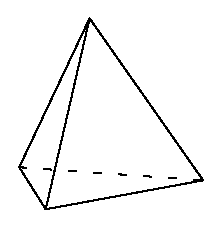
\includegraphics[width=2cm]{figures/platonicsolids1}&
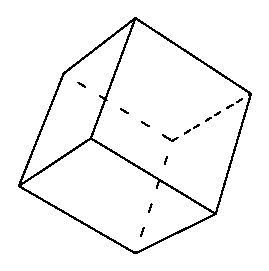
\includegraphics[width=2cm]{figures/platonicsolids2}&
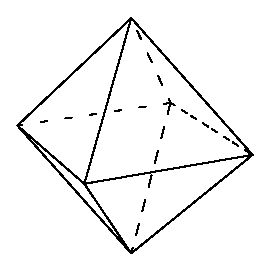
\includegraphics[width=2cm]{figures/platonicsolids3}&
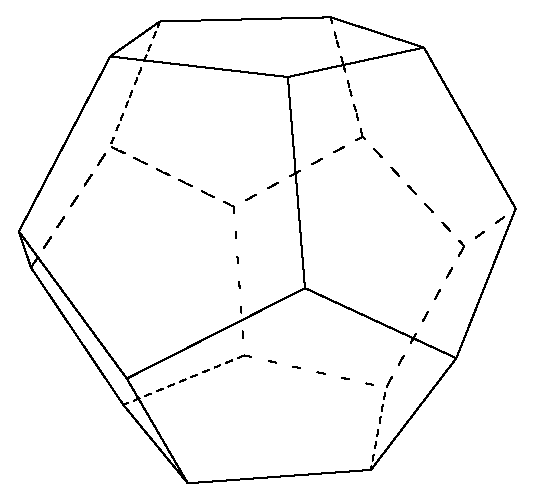
\includegraphics[width=2cm]{figures/platonicsolids4}&
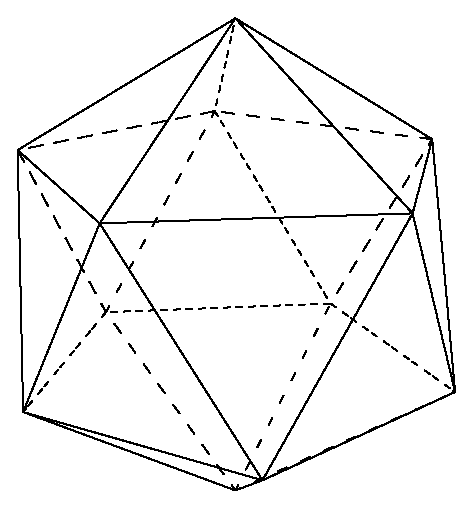
\includegraphics[width=2cm]{figures/platonicsolids5} \end{tabular}\\\bigskip
{\small Figure 1. The \emph{platonic solids} as the five regular convex
3-polytopes.} \end{center}  

 The set of all $k$-faces of $P$ is called the \emph{$k$-skeleton} of $P$, written as  $\operatorname{skel}_k(P).$    \begin{center} 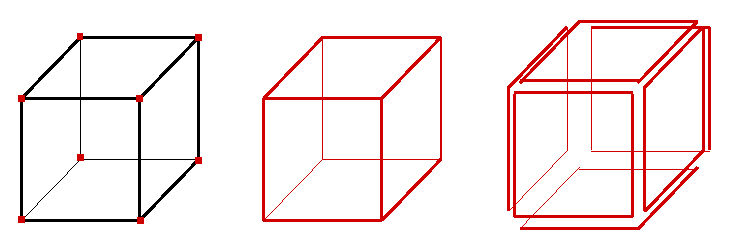
\includegraphics[width=8cm]{figures/skelcube}\\\bigskip {\small
Figure 2. From left to right, drawn in grey: the 0-skeleton, the 1-skeleton
and the 2-skeleton of the cube.} \end{center}  

 A \emph{polytopal complex} $C$ is a finite collection of polytopes $P_i$, $1 \leq i \leq n$ for which the intersection of any two polytopes $P_i \cap P_j$ is either empty or a common face of $P_i$ and $P_j$. The polytopes of maximal dimension are called the \emph{facets} of $C$. The \emph{dimension} of a polytopal complex $C$ is defined as the maximum over all dimensions of its facets. 

 For every $d$-dimensional polytopal complex the $(d+1)$-tuple, containing its number of $i$-faces in the $i$-th entry is called the \emph{$f$-vector} of the polytopal complex. 

 Every polytope $P$ gives rise to a polytopal complex consisting of all the proper faces of $P$. This polytopal complex is called the \emph{boundary complex $C(\partial P)$ of the polytope $P$}. 

  Figure 2 below shows the boundary complex of the cube. \begin{center}
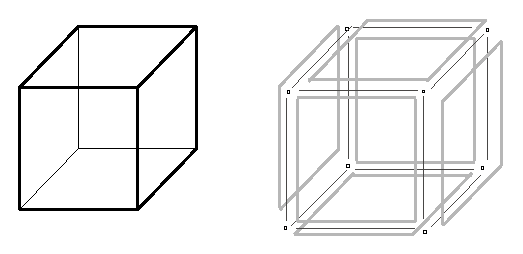
\includegraphics[width=8cm]{figures/cubecomplex}\\\bigskip {\small Figure 3.
The 3-cube (left) and its boundary complex (right) where the 0-faces shown in
black, the 1-faces dark gray and the 2-faces in light gray.} \end{center}  }


\section{\textcolor{Chapter }{Simplices and simplicial complexes}}\label{sec:simplex}
\logpage{[ 2, 2, 0 ]}
\hyperdef{L}{X7AA9180F7CF65B41}{}
{
 A $d$-dimensional \emph{simplex} or \emph{$d$-simplex} for short is the convex hull of $d+1$ points in $E^d$ in general position. Thus the $d$-simplex is the smallest (with respect to the number of vertices) possible $d$-polytope. Every face of the $d$-simplex is a $m$-simplex, $m \leq d$. 

 A 0-simplex is a point, a $1$-simplex is a line segment, a $2$-simplex is a triangle, a $3$-simplex a tetrahedron, and so on. 

  \begin{center} 
\includegraphics[width=10cm]{figures/simplices}\\\bigskip
{\small Figure 4. From left to right: a 0-simplex, a 1-simplex, a 2-simplex, a
3-simplex and a Schlegel diagram of a 4-simplex.} \end{center}  

 A polytopal complex which entirely consists of simplices is called a \emph{simplicial complex} (for this it actually suffices that the facets (i. e., the faces that are not
included in any other face of the complex) of a polytopal complex are
simplices). 

  \begin{center} 
\includegraphics[height=4cm]{figures/simplcompl}\\\bigskip
{\small Figure 4. A simplicial complex (left) and a collection of simplices
that does not form a simplicial complex (right).} \end{center}  

 The dimension of a simplicial complex is the maximal dimension of a facet. A
simplicial complex is said to be \emph{pure} if all facets are of the same dimension. A pure simplicial complex of
dimension $d$ satisfies the \emph{weak pseudomanifold property} if every $(d-1)$-face is part of exactly two facets. 

 Since simplices are polytopes and, hence, simplicial complexes are polytopal
complexes all of the terminology regarding simplicial complexes can be
transfered from polytope theory. }


\section{\textcolor{Chapter }{From geometry to combinatorics}}\label{sec:geomcomb}
\logpage{[ 2, 3, 0 ]}
\hyperdef{L}{X84B178117BE7DD1C}{}
{
 Every $d$-simplex has an \emph{underlying set} in $E^d$, as the set of all points of that simplex. In the same way one can define the \emph{underlying set} $|C|$ of a simplicial complex $C$. If the underlying set of a simplicial complex $C$ is a topological manifold, then $C$ is called \emph{triangulated manifold} (or \emph{triangulation of $|C|$}). 

 One can also go the other way and assign an abstract simplicial complex to a
geometrical one by identifying each simplex with its vertex set. This
obviously defines a set of sets with a natural partial ordering given by the
inclusion (a socalled \emph{poset}). 

  \begin{center} 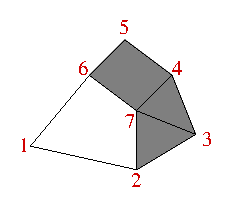
\includegraphics[height=3.5cm]{figures/hasse_complex}\quad
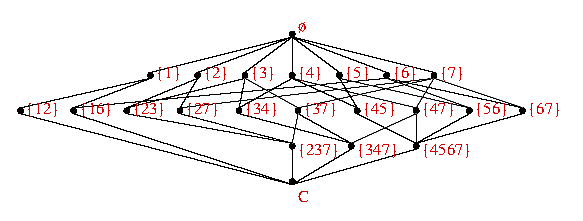
\includegraphics[height=3.5cm]{figures/hasse_diagram}\\\bigskip {\small Figure
5. A geometrical polytopal complex (left) and its abstract version in form of
a poset (right).} \end{center}  

 Let $v$ be a vertex of $C$. The set of all facets that contain $v$ is called \emph{star of $v$ in $C$} and is denoted by star$_C(v)$. The subcomplex of star$_C(v)$ that contains all faces not containing $v$ is called \emph{link of $v$ in $C$}, written as lk$_C(v)$. 

 

 A \emph{combinatorial $d$-manifold} is a $d$-dimensional simplicial complex whose vertex links are all triangulated $(d-1)$-dimensional spheres with standard PL-structure. A \emph{combinatorial pseudomanifold} is a simplicial complex whose vertex links are all combinatorial $(d-1)$-manifolds. 

  \begin{center}
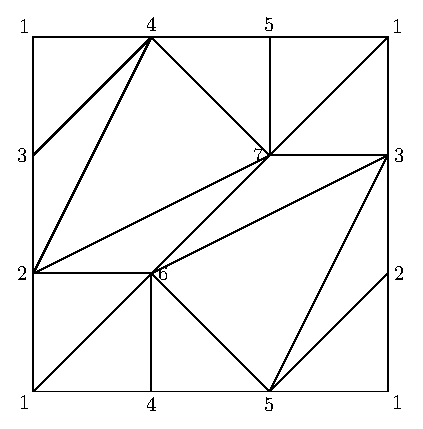
\includegraphics[height=.5\textwidth]{figures/moebius}\\\bigskip {\small
Figure 6. A simplicial complex that is a vertex-minimal combinatorial
triangulation of the torus $T^2$ (so called M\"obius' torus) -- each vertex
link is a hexagon.} \end{center}  

 Note that every combinatorial manifold is a triangulated manifold. The
opposite is wrong: for example, there exists a triangulation of the $5$-sphere that is not combinatorial, the so called \emph{Edward's sphere}, see \cite{Bjoerner00SimplMnfBistellarFlips}. 

 A combinatorial manifold carries an induced PL-structure and can be understood
in terms of an abstract simplicial complex. If the complex has $d$ vertices there exists a natural embedding of $C$ into the $(d-1)$ simplex and, thus, into $E^{d-1}$. In general, there is no canonical embedding into any lower dimensional
space. However, combinatorial methods allow to examine a given simplicial
complex independently from an embedding and, in particular, independently from
vertex coordinates. 

 Some fundamental properties of an abstract simplicial complex $C$ are the following: 
\begin{description}
\item[{Dimensionality.}] The dimension of $C$.
\item[{$f$, $g$ and $h$-vector.}]  The $f$-vector ($f_k$ equals the number of $k$-faces of a simplicial complex), the $g$- and $h$-vector can be obtained from the $f$-vector via linear transformations.
\item[{(Co-)Homology.}] The simplicical (co-)homology groups and Betti numbers.
\item[{Euler characteristic}] The Euler characteristic as the alternating sum over the Betti numbers / the $f$-vector.
\item[{Connectedness and closedness.}] Whether $C$ is strongly connected, path connected, has a boundary or not.
\item[{Symmetries.}] The automorphism group, i. e. the group of all permutations on the set of
vertex labels that do not change the complex as a whole.
\end{description}
 

 All of those properties and many more can be computed on a strictly
combinatorial basis. }


\section{\textcolor{Chapter }{Discrete Normal surfaces}}\label{sec:NormSurfTheory}
\logpage{[ 2, 4, 0 ]}
\hyperdef{L}{X7BE7221B7C38B27D}{}
{
 The concept of \emph{normal surfaces} is originally due to Kneser \cite{Kneser29ClosedSurfIn3Mflds} and Haken \cite{Haken61TheoNormFl}: A surface $S$, properly embedded into a $3$-manifold $M$, is said to be \emph{normal}, if it respects a given cell decomposition of $M$ in the following sense: It does not intersect any vertex nor touch any $3$-cell of the manifold and does not intersect with any $2$-cell in a circle or an arc starting and ending in a point of the same edge.
Here we will look at normal surfaces in the case that $M$ is given as a combinatorial $3$-manifold and we will call the corresponding objects \emph{discrete normal surfaces}. In order to do this let us first define:\\
\\
 \textsc{Definition}\\
 A \emph{polytopal manifold} is a polytopal complex $M$ such that there exists a simplicial subdivision of $M$ which is a combinatorial manifold. If $M$ is a surface we will call it a \emph{polytopal map}. If, in addition $M$ entirely consists of $m$-gons, we call it a \emph{polytopal $m$-gon map}.\\
\\
 \textsc{Definition} (Discrete Normal surface, \cite{Spreer10NormSurfsCombSlic})\\
 Let $M$ be a combinatorial $3$-manifold ($3$-pseudomanifold), $\Delta \in M$ one of its tetrahedra and $P$ the intersection of $\Delta$ with a plane that does not include any vertex of $\Delta$. Then $P$ is called a \emph{normal subset} of $\Delta$. Up to an isotopy that respects the face lattice of $\Delta$, $P$ is equal to one of the triangles $P_{i}$, $1 \leq i \leq 4$, or quadrilaterals $P_{i}$, $5 \leq i \leq 7$, shown in Figure 7. \\
\\
 A polyhedral map $S \subset M$ that entirely consists of facets $P_{i}$ such that every tetrahedron contains at most one facet is called \emph{discrete normal surface} of $M$.\\
\\
 The second author has recently investigated on the combinatorial theory of
discrete normal surfaces, see \cite{Spreer10NormSurfsCombSlic}. 

  \medskip  

  \begin{center}
\includegraphics[width=.8\textwidth]{figures/haken.pdf}\\\bigskip {\small
Figure 7. The seven different normal subsets of the tetrahedron. Note that the
rightmost picture of the bottom row can not be part of a discrete normal
surface.} \end{center}  }

 
\section{\textcolor{Chapter }{Polyhedral Morse theory and slicings}}\label{sec:MorseTheory}
\logpage{[ 2, 5, 0 ]}
\hyperdef{L}{X86275D5979B4B531}{}
{
  In the field of PL-topology K{\"u}hnel developed what one might call a
polyhedral Morse theory (compare \cite{Kuehnel95TightPolySubm}, not to be confused with Forman's discrete Morse theory for cell complexes \cite{Forman95DiscrMorseTheoryCellCompl}):\\
\\
 Let $M$ be a combinatorial $d$-manifold. A function $f:M \to \mathbb{R}$ is called \emph{regular simplexwise linear (rsl)} if $f(v) \neq f(w)$ for any two vertices $w \neq v$ and if $f$ is linear when restricted to an arbitrary simplex of the triangulation.\\
\\
 A vertex $x \in M$ is said to be \emph{critical} for an rsl-function $f:M \to \mathbb{R}$, if $H_{\star} (M_x , M_x \backslash \{ x \} , F) \neq 0$ where $M_x := \{ y \in M | f(y) \leq f(x) \}$ and $F$ is a field.\\
\\
 It follows that no point of $M$ can be critical except possibly the vertices. In arbitrary dimensions we
define:\\
\\
 \textsc{Definition} (Slicing, \cite{Spreer10NormSurfsCombSlic})\\
 Let $M$ be a combinatorial pseudomanifold of dimension $d$ and $f:M \to \mathbb{R}$ an rsl-function. Then we call the pre-image $f^{-1} (\alpha)$ a \emph{slicing} of $M$ whenever $\alpha \neq f(v)$ for any vertex $v \in M$.\\
\\
 By construction, a slicing is a polytopal $(d-1)$-manifold and for any ordered pair $\alpha \leq \beta$ we have $f^{-1} (\alpha) \cong f^{-1} (\beta)$ whenever $f^{-1}([\alpha,\beta])$ contains no vertex of $M$. In particular, a slicing $S$ of a closed combinatorial $3$-manifold $M$ is a discrete normal surface: It follows from the simplexwise linearity of $f$ that the intersection of the pre-image with any tetrahedron of $M$ either forms a single triangle or a single quadrilateral. In addition, if two
facets of $S$ lie in adjacent tetrahedra they either are disjoint or glued together along
the intersection line of the pre-image and the common triangle.\\
\\
 Any partition of the set of vertices $V = V_1 \dot{\cup} V_2 $ of $M$ already determines a slicing: Just define an rsl-function $f: M \to \mathbb{R}$ with $f(v) \leq f(w)$ for all $v \in V_1$ and $w \in V_2$ and look at a suitable pre-image. In the following we will write $S_{(V_1,V_2)}$ for the slicing defined by the vertex partition $V = V_1 \dot{\cup} V_2 $.\\
\\
 Every vertex of a slicing is given as an intersection point of the
corresponding pre-image with an edge $\langle u,w \rangle$ of the combinatorial manifold. Since there is at most one such intersection
point per edge, we usually label this vertex of the slicing according to the
vertices of the corresponding edge, that is $\binom{u}{w}$ with $u \in V_1$ and $w \in V_2$.\\
\\
 Every slicing decomposes the surrounding combinatorial manifold $M$ into at least $2$ pieces (an upper part $M^+$ and a lower part $M^-$). This is not the case for discrete normal surfaces (see \ref{sec:NormSurfTheory}) in general. However, we will focus on the case where discrete normal
surfaces are slicings and we will apply the above notation for both types of
objects.\\
\\
 Since every combinatorial pseudomanifold $M$ has a finite number of vertices, there exist only a finite number of slicings
of $M$. Hence, if $f$ is chosen carefully, the induced slicings admit a useful visualization of $M$, c.f. \cite{Spreer09CombPorpsOfK3}.

  \medskip  

  \begin{center}
\includegraphics[width=.8\textwidth]{figures/slicing.pdf}\\\bigskip {\small
Figure 8. One dimensional slicing of the $2$-sphere (represented as the
boundary of the $3$-simplex) seen as a level set of a regular point of a
simplicial Morse function.} \end{center}  

  \begin{center}
\includegraphics[width=.4\textwidth]{figures/3x3gridtorus.pdf}\\\bigskip
{\small Figure 9. Handlebody decomposition of genus $1$ of a $6$-vertex
$3$-sphere - a $3 \times 3$-grid torus.} \end{center}  

  \begin{center}
\includegraphics[width=.5\textwidth]{figures/titlepicture.pdf}\\\bigskip
{\small Figure 10. Separating sphere of an $8$-vertex cylinder $S_4^2 \times
[0,1]$ - A cuboctahedron (drawn as a Schlegel diagram of a quadrilateral
face).} \end{center}  }

 
\section{\textcolor{Chapter }{Tightness and tight triangulations}}\label{sec:tight}
\logpage{[ 2, 6, 0 ]}
\hyperdef{L}{X842354467CE73393}{}
{
 Tightness is a notion developed in the field of differential geometry as the
equality of the (normalized) \emph{total absolute curvature} of a submanifold with the lower bound \emph{sum of the Betti numbers} \cite{Kuiper84GeomTotAbsCurvTheo}, \cite{Banchoff97TightSubmSmoothPoly}. It was first studied by Alexandrov, Milnor, Chern and Lashof and Kuiper and
later extended to the polyhedral case by Banchoff \cite{Banchoff65TightEmb3DimPolyMnf}, Kuiper \cite{Kuiper84GeomTotAbsCurvTheo} and K{\"u}hnel \cite{Kuehnel95TightPolySubm}. From a geometrical point of view, tightness can be understood as a
generalization of the concept of convexity that applies to objects other than
topological balls and their boundary manifolds since it roughly means that an
embedding of a submanifold is ``as convex as possible'' according to its
topology. The usual definition is the following:\\
\\
 \textsc{Definition} (Tightness, \cite{Kuehnel95TightPolySubm})\\
 Let $\mathbb{F}$ be a field. An embedding $M \rightarrow \mathbb{E}^N$ of a compact manifold is called \emph{$k$-tight with respect to $\mathbb{F}$} if for any open or closed halfspace $h\subset E^N$ the induced homomorphism 
\[H_i(M\cap h;\mathbb{F})\longrightarrow H_i(M;\mathbb{F})\]
 is injective for all $i\leq k$. $M$ is called $\mathbb{F}$\emph{-tight} if it is $k$-tight for all $k$. The standard choice for the field of coefficients is $\mathbb{F}_2$ and an $\mathbb{F}_2$-tight embedding is called \emph{tight}.\\
\\
 With regard to PL embeddings of PL manifolds tightness of \emph{combinatorial manifolds} can also be defined via a purely combinatorial condition as follows. For an
introduction to PL topology see \cite{Rourke72IntrPLTop}.\\
\\
 \textsc{Definition} (Tight triangulation \cite{Kuehnel95TightPolySubm})\\
 Let $\mathbb{F}$ be a field. A combinatorial manifold $K$ on $n$ vertices is called \emph{($k$-) tight w.r.t. $\mathbb{F}$} if its canonical embedding $K\subset \Delta^{n-1}\subset E^{n-1}$ is ($k$-)tight w.r.t. $\mathbb{F}$, where $\Delta^{n-1}$ denotes the $(n-1)$-dimensional simplex.\\
\\
 In dimension $d=2$ the following are equivalent for a triangulated surface $S$ on $n$ vertices: (i) $S$ has a complete edge graph $K_n$, (ii) $S$ appears as a so called \emph{regular case} in Heawood's Map Color Theorem \cite{Ringel74MapColThm}, compare \cite{Kuehnel95TightPolySubm} and (iii) the induced piecewise linear embedding of $S$ into Euclidean $(n-1)$-space has the two-piece property \cite{Banchoff74TightPolyKBProjPMB}, and it is tight \cite{Kuehnel95TightPolySubm}.\\
\\
 K{\"u}hnel investigated the tightness of combinatorial triangulations of
manifolds also in higher dimensions and codimensions, see \cite{Kuehnel94ManSkelConvPolyt}. It turned out that the tightness of a combinatorial triangulation is closely
related to the concept of \emph{Hamiltonicity} of a polyhedral complexes (see \cite{Kuehnel95TightPolySubm}): A subcomplex $A$ of a polyhedral complex $K$ is called \emph{$k$-Hamiltonian} if $A$ contains the full $k$-dimensional skeleton of $K$ (not to be confused with the notion of a $k$-Hamiltonian graph). This generalization of the notion of a Hamiltonian
circuit in a graph seems to be due to C.Schulz \cite{Schulz94PolyhMnfPoly}. A Hamiltonian circuit then becomes a special case of a $0$-Hamiltonian subcomplex of a $1$-dimensional graph or of a higher-dimensional complex.\\
\\
 A triangulated $2k$-manifold that is a $k$-Hamiltonian subcomplex of the boundary complex of some higher dimensional
simplex is a tight triangulation as K{\"u}hnel \cite{Kuehnel95TightPolySubm} showed. Such a triangulation is also called \emph{$(k+1)$-neighborly triangulation} since any $k+1$ vertices in a $k$-dimensional simplex are common neighbors. Moreover, $(k+1)$-neighborly triangulations of $2k$-manifolds are also referred to as \emph{super-neighborly} triangulations -- in analogy with neighborly polytopes the boundary complex of
a $(2k+1)$-polytope can be at most $k$-neighborly unless it is a simplex. Notice here that combinatorial $2k$-manifolds can go beyond $k$-neighborliness, depending on their topology.\\
\\
 Whereas in the $2$-dimensional case all tight triangulations of surfaces were classified by
Ringel and Jungerman and Ringel, in dimensions $d\geq 3$ there exist only a finite number of known examples of tight triangulations
(see \cite{Kuehnel99CensusTight} for a census) apart from the trivial case of the boundary of a simplex and an
infinite series of triangulations of sphere bundles over the circle due to
K{\"u}hnel \cite{Kuehnel95TightPolySubm}, \cite{Kuehnel86HigherDimCsaszar}. }

 
\section{\textcolor{Chapter }{Simplicial blowups}}\label{sec:Blowups}
\logpage{[ 2, 7, 0 ]}
\hyperdef{L}{X7E1BE673859191F0}{}
{
 The \emph{blowing up process} or \emph{Hopf $\sigma$-process} can be described as the resolution of nodes or ordinary double points of a
complex algebraic variety. This was described by H.\texttt{\symbol{126}}Hopf
in \cite{Hopf1951}, compare \cite{Hirzebruch1953} and \cite{Hauser2000}. From the topological point of view the process consists of cutting out some
subspace and gluing in some other subspace. In complex algebraic geometry one
point is replaced by the projective line $\mathbb{C}P^1 \cong S^2$ of all complex lines through that point. This is often called \emph{blowing up} of the point or just \emph{blowup}. In general the process can be applied to non-singular 4-manifolds and yields
a transformation of a manifold \emph{M} to $M \# (+\mathbb{C}P^2)$ or $M \# (-\mathbb{C}P^2)$, depending on the choice of an orientation. The same construction is possible
for nodes or ordinary double points (a special type of singularities), and
also the ambiguity of the orientation is the same for the blowup process of a
node. Similarly it has been used in arbitrary even dimension by Spanier \cite{Spanier56HomKummerMnf} as a so-called \emph{dilatation process}.\\
\\
 A PL version of the blowing up process is the following: We cut out the star
of one of the singular vertices which is, in the case of an ordinary double
point, nothing but a cone over a triangulated $\mathbb{R}P^3$. The boundary of the resulting space is this triangulated $\mathbb{R}P^3$. Now we glue back in a triangulated version $\mathbf{C}$ of a complex projective plane with a $4$-ball removed where antipodal points of the boundary are identified. $\mathbf{C}$ is called a triangulated mapping cylinder and by construction its boundary is
PL homeomorphic to $\mathbb{R}P^3$.\\
\\
 For a combinatorial version with concrete triangulations, however, we face the
problem that these two triangulations are not isomorphic. This implies that
before cutting out and gluing in we have to modify the triangulations by
bistellar moves until they coincide:\\
\\
 \textsc{Definition} (Simplicial blowup, \cite{Spreer09CombPorpsOfK3})\\
 Let $v$ be a vertex of a combinatorial $4$-pseudomanifold $M$ whose link is isomorphic with the particular $11$-vertex triangulation of $\mathbb{R}P^3$ which is given by the boundary complex of the triangulated $\mathbf{C}$ given in \cite{Spreer09CombPorpsOfK3}. Let $\psi : \operatorname{lk}(v) \rightarrow \partial\mathbf{C}$ denote such an isomorphism. A simplicial resolution of the singularity $v$ is given by the following construction $M \mapsto \widetilde{M} := (M \setminus \operatorname{star}(v)^\circ)
\cup_{\psi} \mathbf{C}.$\\
\\
 The process is described in more detail in \cite{Spreer09CombPorpsOfK3}. In particular it is used to transform a $4$-dimensional Kummer variety into a K3 surface. }

 }

 
\chapter{\textcolor{Chapter }{The new GAP object types of \textsf{simpcomp}}}\label{chap:objTypes}
\logpage{[ 3, 0, 0 ]}
\hyperdef{L}{X87A7DD0F8138F0DC}{}
{
  In order to meet the particular requirements of piecewise linear geometric
objects and their invariants, \textsf{simpcomp} defines a number of new \textsf{GAP} object types.

 All new object types are derived from the object type \texttt{SCPropertyObject} which is a subtype of \texttt{Record}. It is a \textsf{GAP} object consisting of permanent and temporary attributes. While \textsf{simpcomp} makes use of \textsf{GAP}'s internal attribute caching mechanism for permanent attributes (see below),
this is not the case for temporary ones.

 The temporary properties of a \texttt{SCPropertyObject} can be accessed directly with the functions \texttt{SCPropertyTmpByName} and changed with \texttt{SCPropertyTmpSet}. But this direct access to property objects is discouraged when working with \textsf{simpcomp}, as the internal consistency of the objects cannot be guaranteed when the
properties of the objects are modified in this way.

 Important note: The temporary properties of \texttt{SCPropertyObject} are not used to hold properties (in the \textsf{GAP} sense) of simplicial complexes or other geometric objects. This is done by the
GAP4 type system \cite{Breuer98GAP4TypeSystem}. Instead, the properties handled by \textsf{simpcomp}'s own caching mechanism are used to store changing information, e.g. the
complex library (see Section \ref{chap:libio}) of the package or any other data which possibly is subject to changes (and
thus not suited to be stored by the \textsf{GAP} type system).

 To realize its complex library (see Section \ref{chap:libio}), \textsf{simpcomp} defines a \textsf{GAP} object type \texttt{SCLibRepository} which provides the possibility to store, load, etc. any defined geometric
object to and from the build-in complex library as well as customized user
libraries. In addition, a searching mechanism is provided.

 Geometric objects are represented by the \textsf{GAP} object type \texttt{SCPolyhedralComplex}, which as well is a subtype of \texttt{SCPropertyObject}. \texttt{SCPolyhedralComplex} is designed to represent any kind of piecewise linear geometric object given
by a certain cell decomposition. Here, as already mentioned, the GAP4 type
system \cite{Breuer98GAP4TypeSystem} is used to cache properties of the object. In this way, a property is not
calculated multiple times in case the object is not altered (see \texttt{SCPropertiesDropped} (\ref{SCPropertiesDropped}) for a way of dropping previously calculated properties).

 As of Version 1.4, \textsf{simpcomp} makes use of two different subtypes of \texttt{SCPolyhedralComplex}: \texttt{SCSimplicialComplex} to handle simplicial complexes and \texttt{SCNormalSurface} to deal with discrete normal surfaces (slicings of dimension 2). Whenever
possible, only one method per operations is implemented to deal with all
subtypes of \texttt{SCPolyhedralComplex}, these functions are described in Chapter \ref{chap:polyhedralcomplex}. For all other operations, the different methods for \texttt{SCSimplicialComplex} and \texttt{SCNormalSurface} are documented separately. 
\section{\textcolor{Chapter }{Accessing properties of a \texttt{SCPolyhedralComplex} object}}\label{sec:AcessSC}
\logpage{[ 3, 1, 0 ]}
\hyperdef{L}{X79C7AD47824F17C8}{}
{
  As described above the object type \texttt{SCPolyhedralComplex} (and thus also the \textsf{GAP} object types \texttt{SCSimplicialComplex} and \texttt{SCNormalSurface}) has properties that are handled by the GAP4 type system. Hence, GAP takes
care of the internal consistency of objects of type \texttt{SCSimplicialComplex}.

 There are two ways of accessing properties of a \texttt{SCPolyhedralComplex} object. The first is to call a property handler function of the property one
wishes to calculate. The first argument of such a property handler function is
always the simplicial complex for which the property should be calculated, in
some cases followed by further arguments of the property handler function. An
example would be: 
\begin{Verbatim}[commandchars=!@|,fontsize=\small,frame=single,label=Example]
  !gapprompt@gap>| !gapinput@c:=SCBdSimplex(3);; # create a SCSimplicialComplex object
|
  !gapprompt@gap>| !gapinput@SCFVector(c);
|
  [ 4, 6, 4 ]
  !gapprompt@gap>| !gapinput@SCSkel(c,0);
|
  [ [ 1 ], [ 2 ], [ 3 ], [ 4 ] ]
\end{Verbatim}
 Here the functions \texttt{SCFVector} and \texttt{SCSkel} are the property handler functions, see Chapter \ref{chap:prophandler} for a list of all property handlers of a \texttt{SCPolyhedralComplex}, \texttt{SCSimplicialComplex} or \texttt{SCNormalSurface} object. Apart from this (standard) method of calling the property handlers
directly with a \texttt{SCPolyhedralComplex} object, \textsf{simpcomp} provides the user with another more object oriented method which calls
property handlers of a \texttt{SCPolyhedralComplex} object indirectly and more conveniently: 
\begin{Verbatim}[commandchars=!@|,fontsize=\small,frame=single,label=Example]
  !gapprompt@gap>| !gapinput@c:=SCBdSimplex(3);; # create a SCSimplicialComplex object
|
  !gapprompt@gap>| !gapinput@c.F;
|
  [ 4, 6, 4 ]
  !gapprompt@gap>| !gapinput@c.Skel(0);
|
  [ [ 1 ], [ 2 ], [ 3 ], [ 4 ] ]
\end{Verbatim}
 Note that the code in this example calculates the same properties as in the
first example above, but the properties of a \texttt{SCPolyhedralComplex} object are accessed via the \texttt{.} operator (the record access operator).

 For each property handler of a \texttt{SCPolyhedralComplex} object the object oriented form of this property handler equals the name of
the corresponding operation. However, in most cases abbreviations are
available: Usually the prefix ``\texttt{SC}'' can be dropped, in other cases even shorter names are available. See
Chapter \ref{chap:prophandler} for a complete list of all abbreviations available. }

 

  \begin{center}
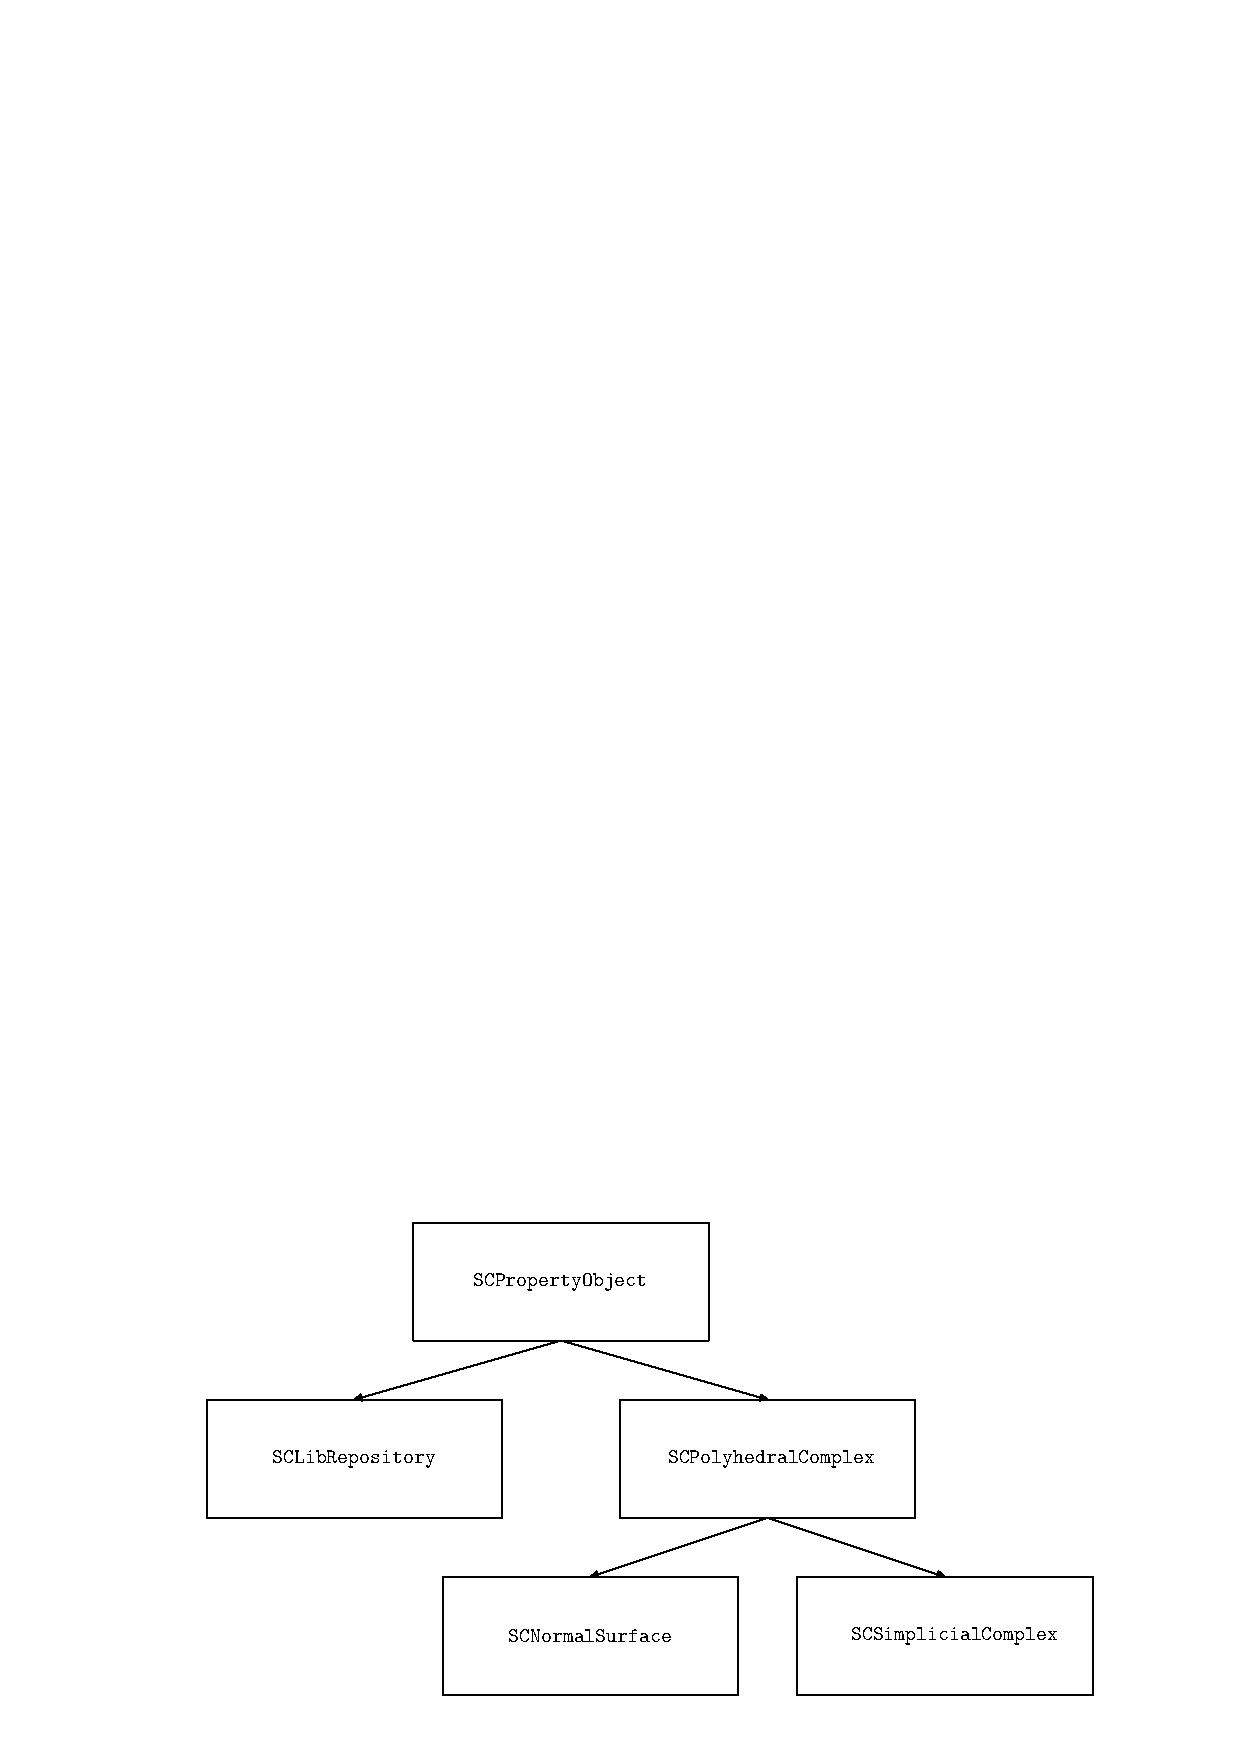
\includegraphics[width=1.0\textwidth]{figures/flowchart.pdf}\\\bigskip {\small
Figure 11. Overview over all GAP object types defined by simpcomp.}
\end{center}  

 }


\chapter{\textcolor{Chapter }{Functions and operations for the GAP object type \texttt{SCPolyhedralComplex}}}\label{chap:polyhedralcomplex}
\logpage{[ 4, 0, 0 ]}
\hyperdef{L}{X8518F9E57E38598E}{}
{
  In the following all operations for the \textsf{GAP} object type \texttt{SCPolyhedralComplex} are listed. I. e. for the following operations only one method is implemented
to deal with all geometric objects derived from this object type. 
\section{\textcolor{Chapter }{Computing properties of objects of type \texttt{SCPolyhedralComplex}}}\label{sec:PCglprops}
\logpage{[ 4, 1, 0 ]}
\hyperdef{L}{X82F92CD2813A23C9}{}
{
  The following functions compute basic properties of objects of type \texttt{SCPolyhedralComplex} (and thus also of objects of type \texttt{SCSimplicialComplex} and \texttt{SCNormalSurface}). None of these functions alter the complex. All properties are returned as
immutable objects (this ensures data consistency of the cached properties of a
simplicial complex). Use \texttt{ShallowCopy} or the internal \textsf{simpcomp} function \texttt{SCIntFunc.DeepCopy} to get a mutable copy.

 Note: every object is internally stored with the standard vertex labeling from $1$ to $n$ and a maptable to restore the original vertex labeling. Thus, we have to
relabel some of the complex properties (facets, etc...) whenever we want to
return them to the user. As a consequence, some of the functions exist twice,
one of them with the appendix "Ex". These functions return the standard
labeling whereas the other ones relabel the result to the original labeling. 

\subsection{\textcolor{Chapter }{SCFacets}}
\logpage{[ 4, 1, 1 ]}\nobreak
\hyperdef{L}{X7BDD568184E3419D}{}
{\noindent\textcolor{FuncColor}{$\triangleright$\ \ \texttt{SCFacets({\mdseries\slshape complex})\index{SCFacets@\texttt{SCFacets}}
\label{SCFacets}
}\hfill{\scriptsize (method)}}\\
\textbf{\indent Returns:\ }
 a facet list upon success, \texttt{fail} otherwise.



 Returns the facets of a simplicial complex in the original vertex labeling. 
\begin{Verbatim}[commandchars=!@|,fontsize=\small,frame=single,label=Example]
   gap> c:=SC([[2,3],[3,4],[4,2]]);;
   gap> SCFacets(c);
   [ [ 2, 3 ], [ 2, 4 ], [ 3, 4 ] ]
   
\end{Verbatim}
 }

 

\subsection{\textcolor{Chapter }{SCFacetsEx}}
\logpage{[ 4, 1, 2 ]}\nobreak
\hyperdef{L}{X87DC942881235E25}{}
{\noindent\textcolor{FuncColor}{$\triangleright$\ \ \texttt{SCFacetsEx({\mdseries\slshape complex})\index{SCFacetsEx@\texttt{SCFacetsEx}}
\label{SCFacetsEx}
}\hfill{\scriptsize (method)}}\\
\textbf{\indent Returns:\ }
 a facet list upon success, \texttt{fail} otherwise.



 Returns the facets of a simplicial complex as they are stored, i. e. with
standard vertex labeling from 1 to n. 
\begin{Verbatim}[commandchars=!@|,fontsize=\small,frame=single,label=Example]
   gap> c:=SC([[2,3],[3,4],[4,2]]);;
   gap> SCFacetsEx(c);
   [ [ 1, 2 ], [ 1, 3 ], [ 2, 3 ] ]
   
\end{Verbatim}
 }

 

\subsection{\textcolor{Chapter }{SCVertices}}
\logpage{[ 4, 1, 3 ]}\nobreak
\hyperdef{L}{X849B0CD0796298EA}{}
{\noindent\textcolor{FuncColor}{$\triangleright$\ \ \texttt{SCVertices({\mdseries\slshape complex})\index{SCVertices@\texttt{SCVertices}}
\label{SCVertices}
}\hfill{\scriptsize (method)}}\\
\textbf{\indent Returns:\ }
 a list of vertex labels of \mbox{\texttt{\mdseries\slshape complex}} upon success, \texttt{fail} otherwise.



 Returns the vertex labels of a simplicial complex \mbox{\texttt{\mdseries\slshape complex}}. 
\begin{Verbatim}[commandchars=!@|,fontsize=\small,frame=single,label=Example]
   gap> sphere:=SC([["x",45,[1,1]],["x",45,["b",3]],["x",[1,1],
     ["b",3]],[45,[1,1],["b",3]]]);;
   gap> SCVerticesEx(sphere);
   [ 1 .. 4 ]
   gap> SCVertices(sphere);
   [ 45, [ 1, 1 ], "x", [ "b", 3 ] ]
   
\end{Verbatim}
 }

 

\subsection{\textcolor{Chapter }{SCVerticesEx}}
\logpage{[ 4, 1, 4 ]}\nobreak
\hyperdef{L}{X83D02BCD7D19FC6F}{}
{\noindent\textcolor{FuncColor}{$\triangleright$\ \ \texttt{SCVerticesEx({\mdseries\slshape complex})\index{SCVerticesEx@\texttt{SCVerticesEx}}
\label{SCVerticesEx}
}\hfill{\scriptsize (method)}}\\
\textbf{\indent Returns:\ }
 $[ 1, \ldots , n ]$ upon success, \texttt{fail} otherwise.



 Returns $\left[1, \ldots , n \right]$, where $n$ is the number of vertices of a simplicial complex \mbox{\texttt{\mdseries\slshape complex}}. 
\begin{Verbatim}[commandchars=!@|,fontsize=\small,frame=single,label=Example]
   gap> c:=SC([[1,4,5],[4,9,8],[12,13,14,15,16,17]]);;
   gap> SCVerticesEx(c);
   [ 1 .. 11 ]
   
\end{Verbatim}
 }

 }


\section{\textcolor{Chapter }{Vertex labelings and label operations}}\logpage{[ 4, 2, 0 ]}
\hyperdef{L}{X7B69B61E867E748E}{}
{
  This section focuses on functions operating on the labels of a complex such as
the name or the vertex labeling.

 Internally, \textsf{simpcomp} uses the standard labeling $[1, \ldots , n]$. It is recommended to use simple vertex labels like integers and, whenever
possible, the standard labeling, see also \texttt{SCRelabelStandard} (\ref{SCRelabelStandard}). 

\subsection{\textcolor{Chapter }{SCLabelMax}}
\logpage{[ 4, 2, 1 ]}\nobreak
\hyperdef{L}{X7C02CB9E8422EEE8}{}
{\noindent\textcolor{FuncColor}{$\triangleright$\ \ \texttt{SCLabelMax({\mdseries\slshape complex})\index{SCLabelMax@\texttt{SCLabelMax}}
\label{SCLabelMax}
}\hfill{\scriptsize (method)}}\\
\textbf{\indent Returns:\ }
vertex label of \mbox{\texttt{\mdseries\slshape complex}} (an integer, a short list, a character, a short string) upon success, \texttt{fail} otherwise.



 The maximum over all vertex labels is determined by the \textsf{GAP} function \texttt{MaximumList}. 
\begin{Verbatim}[commandchars=!@|,fontsize=\small,frame=single,label=Example]
   gap> c:=SCBdSimplex(3);;
   gap> SCRelabel(c,[10,100,100000,3500]);;
   gap> SCLabelMax(c);
   100000
   
\end{Verbatim}
 
\begin{Verbatim}[commandchars=!@|,fontsize=\small,frame=single,label=Example]
   gap> c:=SCBdSimplex(3);;
   gap> SCRelabel(c,["a","bbb",5,[1,1]]);;
   gap> SCLabelMax(c);
   "bbb"
   
\end{Verbatim}
 }

 

\subsection{\textcolor{Chapter }{SCLabelMin}}
\logpage{[ 4, 2, 2 ]}\nobreak
\hyperdef{L}{X7FC2186B7D346BD3}{}
{\noindent\textcolor{FuncColor}{$\triangleright$\ \ \texttt{SCLabelMin({\mdseries\slshape complex})\index{SCLabelMin@\texttt{SCLabelMin}}
\label{SCLabelMin}
}\hfill{\scriptsize (method)}}\\
\textbf{\indent Returns:\ }
vertex label of \mbox{\texttt{\mdseries\slshape complex}} (an integer, a short list, a character, a short string) upon success, \texttt{fail} otherwise.



 The minimum over all vertex labels is determined by the \textsf{GAP} function \texttt{MinimumList}. 
\begin{Verbatim}[commandchars=!@|,fontsize=\small,frame=single,label=Example]
   gap> c:=SCBdSimplex(3);;
   gap> SCRelabel(c,[10,100,100000,3500]);;
   gap> SCLabelMin(c);
   10
   
\end{Verbatim}
 
\begin{Verbatim}[commandchars=!@|,fontsize=\small,frame=single,label=Example]
   gap> c:=SCBdSimplex(3);;
   gap> SCRelabel(c,["a","bbb",5,[1,1]]);;
   gap> SCLabelMin(c);
   5
   
\end{Verbatim}
 }

 

\subsection{\textcolor{Chapter }{SCLabels}}
\logpage{[ 4, 2, 3 ]}\nobreak
\hyperdef{L}{X826E9B4482AF2671}{}
{\noindent\textcolor{FuncColor}{$\triangleright$\ \ \texttt{SCLabels({\mdseries\slshape complex})\index{SCLabels@\texttt{SCLabels}}
\label{SCLabels}
}\hfill{\scriptsize (method)}}\\
\textbf{\indent Returns:\ }
a list of vertex labels of \mbox{\texttt{\mdseries\slshape complex}} (a list of integers, short lists, characters, short strings, ...) upon
success, \texttt{fail} otherwise.



 Returns the vertex labels of \mbox{\texttt{\mdseries\slshape complex}} as a list. This is a synonym of \texttt{SCVertices} (\ref{SCVertices}). 
\begin{Verbatim}[commandchars=!@|,fontsize=\small,frame=single,label=Example]
   gap> c:=SCFromFacets(Combinations(["a","b","c","d"],3));;
   gap> SCLabels(c);
   [ "a", "b", "c", "d" ]
   
\end{Verbatim}
 }

 

\subsection{\textcolor{Chapter }{SCName}}
\logpage{[ 4, 2, 4 ]}\nobreak
\hyperdef{L}{X81C8A7EC84F5DEE9}{}
{\noindent\textcolor{FuncColor}{$\triangleright$\ \ \texttt{SCName({\mdseries\slshape complex})\index{SCName@\texttt{SCName}}
\label{SCName}
}\hfill{\scriptsize (operation)}}\\
\textbf{\indent Returns:\ }
 a string upon success, \texttt{fail} otherwise.



 Returns the name of a simplicial complex \mbox{\texttt{\mdseries\slshape complex}}. 
\begin{Verbatim}[commandchars=!@|,fontsize=\small,frame=single,label=Example]
   gap> c:=SCBdSimplex(5);;
   gap> SCName(c);
   "S^4_6"
   
\end{Verbatim}
 
\begin{Verbatim}[commandchars=!@|,fontsize=\small,frame=single,label=Example]
   gap> c:=SC([[1,2],[2,3],[3,1]]);;
   gap> SCName(c);
   "unnamed complex 2"
   
\end{Verbatim}
 }

 

\subsection{\textcolor{Chapter }{SCReference}}
\logpage{[ 4, 2, 5 ]}\nobreak
\hyperdef{L}{X7A812340843BCED3}{}
{\noindent\textcolor{FuncColor}{$\triangleright$\ \ \texttt{SCReference({\mdseries\slshape complex})\index{SCReference@\texttt{SCReference}}
\label{SCReference}
}\hfill{\scriptsize (operation)}}\\
\textbf{\indent Returns:\ }
 a string upon success, \texttt{fail} otherwise.



 Returns a literature reference of a polyhedral complex \mbox{\texttt{\mdseries\slshape complex}}. 
\begin{Verbatim}[commandchars=!@|,fontsize=\small,frame=single,label=Example]
   gap> c:=SCLib.Load(253);;
   gap> SCReference(c);
   "F.H.Lutz: 'The Manifold Page', http://www.math.tu-berlin.de/diskregeom/stella\
   r/"
   gap> c:=SC([[1,2],[2,3],[3,1]]);;
   gap> SCReference(c);
   #I  SCReference: complex lacks reference.
   fail
   
\end{Verbatim}
 }

 

\subsection{\textcolor{Chapter }{SCRelabel}}
\logpage{[ 4, 2, 6 ]}\nobreak
\hyperdef{L}{X7B6011907B74EDDA}{}
{\noindent\textcolor{FuncColor}{$\triangleright$\ \ \texttt{SCRelabel({\mdseries\slshape complex, maptable})\index{SCRelabel@\texttt{SCRelabel}}
\label{SCRelabel}
}\hfill{\scriptsize (method)}}\\
\textbf{\indent Returns:\ }
 \texttt{true} upon success, \texttt{fail} otherwise.



 \mbox{\texttt{\mdseries\slshape maptable}} has to be a list of length $n$ where $n$ is the number of vertices of \mbox{\texttt{\mdseries\slshape complex}}. The function maps the $i$-th entry of \mbox{\texttt{\mdseries\slshape maptable}} to the $i$-th entry of the current vertex labels. If \mbox{\texttt{\mdseries\slshape complex}} has the standard vertex labeling $[1, \ldots , n]$ the vertex label $i$ is mapped to \mbox{\texttt{\mdseries\slshape maptable[i]}}.

 Note that the elements of \mbox{\texttt{\mdseries\slshape maptable}} must admit a total ordering. Hence, following Section 4.11 of the \textsf{GAP} manual, they must be members of one of the following families: rationals \texttt{IsRat}, cyclotomics \texttt{IsCyclotomic}, finite field elements \texttt{IsFFE}, permutations \texttt{IsPerm}, booleans \texttt{IsBool}, characters \texttt{IsChar} and lists (strings) \texttt{IsList}.

 Internally the property ``SCVertices'' of \mbox{\texttt{\mdseries\slshape complex}} is replaced by \mbox{\texttt{\mdseries\slshape maptable.}}

 
\begin{Verbatim}[commandchars=!@|,fontsize=\small,frame=single,label=Example]
   gap> list:=SCLib.SearchByAttribute("F[1]=12");; 
   gap> c:=SCLib.Load(list[1][1]);;
   gap> SCVertices(c);
   [ 1, 2, 3, 4, 5, 6, 7, 8, 9, 10, 11, 12 ]
   gap> SCRelabel(c,["a","b","c","d","e","f","g","h","i","j","k","l"]);
   true
   gap> SCLabels(c);
   [ "a", "b", "c", "d", "e", "f", "g", "h", "i", "j", "k", "l" ]
   
\end{Verbatim}
 }

 

\subsection{\textcolor{Chapter }{SCRelabelStandard}}
\logpage{[ 4, 2, 7 ]}\nobreak
\hyperdef{L}{X78E22E3B787DDE90}{}
{\noindent\textcolor{FuncColor}{$\triangleright$\ \ \texttt{SCRelabelStandard({\mdseries\slshape complex})\index{SCRelabelStandard@\texttt{SCRelabelStandard}}
\label{SCRelabelStandard}
}\hfill{\scriptsize (method)}}\\
\textbf{\indent Returns:\ }
 \texttt{true} upon success, \texttt{fail} otherwise.



 Maps vertex labels $v_1 , \ldots , v_n$ of \mbox{\texttt{\mdseries\slshape complex}} to $[1 , \ldots , n]$. Internally the property "SCVertices" is replaced by $[1 , \ldots , n]$. 
\begin{Verbatim}[commandchars=!@|,fontsize=\small,frame=single,label=Example]
   gap> list:=SCLib.SearchByAttribute("F[1]=12");; 
   gap> c:=SCLib.Load(list[1][1]);;
   gap> SCRelabel(c,[4..15]);
   true
   gap> SCVertices(c);
   [ 4 .. 15 ]
   gap> SCRelabelStandard(c);
   true
   gap> SCLabels(c);
   [ 1 .. 12 ]
   
\end{Verbatim}
 }

 

\subsection{\textcolor{Chapter }{SCRelabelTransposition}}
\logpage{[ 4, 2, 8 ]}\nobreak
\hyperdef{L}{X83276FCB844628EC}{}
{\noindent\textcolor{FuncColor}{$\triangleright$\ \ \texttt{SCRelabelTransposition({\mdseries\slshape complex, pair})\index{SCRelabelTransposition@\texttt{SCRelabelTransposition}}
\label{SCRelabelTransposition}
}\hfill{\scriptsize (method)}}\\
\textbf{\indent Returns:\ }
 \texttt{true} upon success, \texttt{fail} otherwise.



 Permutes vertex labels of a single pair of vertices. \mbox{\texttt{\mdseries\slshape pair}} has to be a list of length $2$ and a sublist of the property ``SCVertices''.

 The function is equivalent to \texttt{SCRelabel} (\ref{SCRelabel}) with \mbox{\texttt{\mdseries\slshape maptable}} $= [ SCVertices[1] , \ldots , SCVertices[j] , \ldots , SCVertices[i] , \dots ,
SCVertices[n]]$ if \mbox{\texttt{\mdseries\slshape pair}} $= [ SCVertices[j] , SCVertices[i]]$, $j \leq i$, $j \neq i$.

 
\begin{Verbatim}[commandchars=!@|,fontsize=\small,frame=single,label=Example]
   gap> c:=SCBdSimplex(3);;
   gap> SCVertices(c);
   [ 1, 2, 3, 4 ]
   gap> SCRelabelTransposition(c,[1,2]);;
   gap> SCLabels(c);
   [ 2, 1, 3, 4 ]
   
\end{Verbatim}
 }

 

\subsection{\textcolor{Chapter }{SCRename}}
\logpage{[ 4, 2, 9 ]}\nobreak
\hyperdef{L}{X84AA5E217F1EAE23}{}
{\noindent\textcolor{FuncColor}{$\triangleright$\ \ \texttt{SCRename({\mdseries\slshape complex, name})\index{SCRename@\texttt{SCRename}}
\label{SCRename}
}\hfill{\scriptsize (method)}}\\
\textbf{\indent Returns:\ }
 \texttt{true} upon success, \texttt{fail} otherwise.



 Renames a polyhedral complex. The argument \mbox{\texttt{\mdseries\slshape name}} has to be given in form of a string. 
\begin{Verbatim}[commandchars=!@|,fontsize=\small,frame=single,label=Example]
   gap> c:=SCBdSimplex(5);;
   gap> SCName(c);
   "S^4_6"
   gap> SCRename(c,"mySphere");
   true
   gap> SCName(c);
   "mySphere"
   
\end{Verbatim}
 }

 

\subsection{\textcolor{Chapter }{SCSetReference}}
\logpage{[ 4, 2, 10 ]}\nobreak
\hyperdef{L}{X87184048876229F3}{}
{\noindent\textcolor{FuncColor}{$\triangleright$\ \ \texttt{SCSetReference({\mdseries\slshape complex, ref})\index{SCSetReference@\texttt{SCSetReference}}
\label{SCSetReference}
}\hfill{\scriptsize (method)}}\\
\textbf{\indent Returns:\ }
 \texttt{true} upon success, \texttt{fail} otherwise.



 Sets the literature reference of a polyhedral complex. The argument \mbox{\texttt{\mdseries\slshape ref}} has to be given in form of a string. 
\begin{Verbatim}[commandchars=!@|,fontsize=\small,frame=single,label=Example]
   gap> c:=SCBdSimplex(5);;
   gap> SCReference(c);
   #I  SCReference: complex lacks reference.
   fail
   gap> SCSetReference(c,"my 5-sphere in my cool paper");
   true
   gap> SCReference(c);
   "my 5-sphere in my cool paper"
   
\end{Verbatim}
 }

 

\subsection{\textcolor{Chapter }{SCUnlabelFace}}
\logpage{[ 4, 2, 11 ]}\nobreak
\hyperdef{L}{X80A64720826EA264}{}
{\noindent\textcolor{FuncColor}{$\triangleright$\ \ \texttt{SCUnlabelFace({\mdseries\slshape complex, face})\index{SCUnlabelFace@\texttt{SCUnlabelFace}}
\label{SCUnlabelFace}
}\hfill{\scriptsize (method)}}\\
\textbf{\indent Returns:\ }
 a list upon success, \texttt{fail} otherwise.



 Computes the standard labeling of \mbox{\texttt{\mdseries\slshape face}} in \mbox{\texttt{\mdseries\slshape complex}}. 
\begin{Verbatim}[commandchars=!@|,fontsize=\small,frame=single,label=Example]
   gap> c:=SCBdSimplex(3);;
   gap> SCRelabel(c,["a","bbb",5,[1,1]]);;
   gap> SCUnlabelFace(c,["a","bbb",5]);
   [ 1, 2, 3 ]
   
\end{Verbatim}
 }

 }


\section{\textcolor{Chapter }{Operations on objects of type \texttt{SCPolyhedralComplex}}}\logpage{[ 4, 3, 0 ]}
\hyperdef{L}{X7FC0D9B48426427F}{}
{
  The following functions perform operations on objects of type \texttt{SCPolyhedralComplex} and all of its subtypes. Most of them return simplicial complexes. Thus, this
section is closely related to the Sections \ref{sec:generateFromOld} (for objects of type \texttt{SCSimplicialComplex}), ''Generate new complexes from old''. However, the data generated here is
rather seen as an intrinsic attribute of the original complex and not as an
independent complex. 

\subsection{\textcolor{Chapter }{SCAntiStar}}
\logpage{[ 4, 3, 1 ]}\nobreak
\hyperdef{L}{X84646E6786FB7993}{}
{\noindent\textcolor{FuncColor}{$\triangleright$\ \ \texttt{SCAntiStar({\mdseries\slshape complex, face})\index{SCAntiStar@\texttt{SCAntiStar}}
\label{SCAntiStar}
}\hfill{\scriptsize (method)}}\\
\textbf{\indent Returns:\ }
 simplicial complex of type \texttt{SCSimplicialComplex} upon success, \texttt{fail} otherwise .



 Computes the anti star of \mbox{\texttt{\mdseries\slshape face}} (a face given as a list of vertices or a scalar interpreted as vertex) in \mbox{\texttt{\mdseries\slshape complex}}, i. e. the complement of \mbox{\texttt{\mdseries\slshape face}} in \mbox{\texttt{\mdseries\slshape complex}}. 
\begin{Verbatim}[commandchars=!@|,fontsize=\small,frame=single,label=Example]
   gap> SCLib.SearchByName("RP^2");     
   [ [ 3, "RP^2 (VT)" ], [ 635, "RP^2xS^1" ] ]
   gap> rp2:=SCLib.Load(last[1][1]);;
   gap> SCVertices(rp2);
   [ 1, 2, 3, 4, 5, 6 ]
   gap> SCAntiStar(rp2,1);
   [SimplicialComplex
   
    Properties known: Dim, FacetsEx, Name, Vertices.
   
    Name="ast([ 1 ]) in RP^2 (VT)"
    Dim=2
   
   /SimplicialComplex]
   gap> last.Facets;
   [ [ 2, 3, 4 ], [ 2, 4, 5 ], [ 2, 5, 6 ], [ 3, 4, 6 ], [ 3, 5, 6 ] ]
   
\end{Verbatim}
 }

 

\subsection{\textcolor{Chapter }{SCLink}}
\logpage{[ 4, 3, 2 ]}\nobreak
\hyperdef{L}{X874059937F4C709B}{}
{\noindent\textcolor{FuncColor}{$\triangleright$\ \ \texttt{SCLink({\mdseries\slshape complex, face})\index{SCLink@\texttt{SCLink}}
\label{SCLink}
}\hfill{\scriptsize (method)}}\\
\textbf{\indent Returns:\ }
 simplicial complex of type \texttt{SCSimplicialComplex} upon success, \texttt{fail} otherwise.



 Computes the link of \mbox{\texttt{\mdseries\slshape face}} (a face given as a list of vertices or a scalar interpreted as vertex) in a
polyhedral complex \mbox{\texttt{\mdseries\slshape complex}}, i. e. all facets containing \mbox{\texttt{\mdseries\slshape face}}, reduced by \mbox{\texttt{\mdseries\slshape face}}. if \mbox{\texttt{\mdseries\slshape complex}} is pure, the resulting complex is of dimension dim(\mbox{\texttt{\mdseries\slshape complex}}) - dim(\mbox{\texttt{\mdseries\slshape face}}) $-1$. If \mbox{\texttt{\mdseries\slshape face}} is not a face of \mbox{\texttt{\mdseries\slshape complex}} the empty complex is returned. 
\begin{Verbatim}[commandchars=!@|,fontsize=\small,frame=single,label=Example]
   gap> SCLib.SearchByName("RP^2");     
   [ [ 3, "RP^2 (VT)" ], [ 635, "RP^2xS^1" ] ]
   gap> rp2:=SCLib.Load(last[1][1]);;
   gap> SCVertices(rp2);
   [ 1, 2, 3, 4, 5, 6 ]
   gap> SCLink(rp2,[1]);
   [SimplicialComplex
   
    Properties known: Dim, FacetsEx, Name, Vertices.
   
    Name="lk([ 1 ]) in RP^2 (VT)"
    Dim=1
   
   /SimplicialComplex]
   gap> last.Facets;
   [ [ 2, 3 ], [ 2, 6 ], [ 3, 5 ], [ 4, 5 ], [ 4, 6 ] ]
   
\end{Verbatim}
 }

 

\subsection{\textcolor{Chapter }{SCLinks}}
\logpage{[ 4, 3, 3 ]}\nobreak
\hyperdef{L}{X7EFA115B7B26F9AD}{}
{\noindent\textcolor{FuncColor}{$\triangleright$\ \ \texttt{SCLinks({\mdseries\slshape complex, k})\index{SCLinks@\texttt{SCLinks}}
\label{SCLinks}
}\hfill{\scriptsize (method)}}\\
\textbf{\indent Returns:\ }
 a list of simplicial complexes of type \texttt{SCSimplicialComplex} upon success, \texttt{fail} otherwise.



 Computes the link of all \mbox{\texttt{\mdseries\slshape k}}-faces of the polyhedral complex \mbox{\texttt{\mdseries\slshape complex}} and returns them as a list of simplicial complexes. Internally calls \texttt{SCLink} (\ref{SCLink}) for every \mbox{\texttt{\mdseries\slshape k}}-face of \mbox{\texttt{\mdseries\slshape complex}}. 
\begin{Verbatim}[commandchars=!@|,fontsize=\small,frame=single,label=Example]
   gap> c:=SCBdSimplex(4);;
   gap> SCLinks(c,0);
   [ [SimplicialComplex
       
        Properties known: Dim, FacetsEx, Name, Vertices.
       
        Name="lk([ 1 ]) in S^3_5"
        Dim=2
       
       /SimplicialComplex], [SimplicialComplex
       
        Properties known: Dim, FacetsEx, Name, Vertices.
       
        Name="lk([ 2 ]) in S^3_5"
        Dim=2
       
       /SimplicialComplex], [SimplicialComplex
       
        Properties known: Dim, FacetsEx, Name, Vertices.
       
        Name="lk([ 3 ]) in S^3_5"
        Dim=2
       
       /SimplicialComplex], [SimplicialComplex
       
        Properties known: Dim, FacetsEx, Name, Vertices.
       
        Name="lk([ 4 ]) in S^3_5"
        Dim=2
       
       /SimplicialComplex], [SimplicialComplex
       
        Properties known: Dim, FacetsEx, Name, Vertices.
       
        Name="lk([ 5 ]) in S^3_5"
        Dim=2
       
       /SimplicialComplex] ]
   gap> SCLinks(c,1);
   [ [SimplicialComplex
       
        Properties known: Dim, FacetsEx, Name, Vertices.
       
        Name="lk([ 1, 2 ]) in S^3_5"
        Dim=1
       
       /SimplicialComplex], [SimplicialComplex
       
        Properties known: Dim, FacetsEx, Name, Vertices.
       
        Name="lk([ 1, 3 ]) in S^3_5"
        Dim=1
       
       /SimplicialComplex], [SimplicialComplex
       
        Properties known: Dim, FacetsEx, Name, Vertices.
       
        Name="lk([ 1, 4 ]) in S^3_5"
        Dim=1
       
       /SimplicialComplex], [SimplicialComplex
       
        Properties known: Dim, FacetsEx, Name, Vertices.
       
        Name="lk([ 1, 5 ]) in S^3_5"
        Dim=1
       
       /SimplicialComplex], [SimplicialComplex
       
        Properties known: Dim, FacetsEx, Name, Vertices.
       
        Name="lk([ 2, 3 ]) in S^3_5"
        Dim=1
       
       /SimplicialComplex], [SimplicialComplex
       
        Properties known: Dim, FacetsEx, Name, Vertices.
       
        Name="lk([ 2, 4 ]) in S^3_5"
        Dim=1
       
       /SimplicialComplex], [SimplicialComplex
       
        Properties known: Dim, FacetsEx, Name, Vertices.
       
        Name="lk([ 2, 5 ]) in S^3_5"
        Dim=1
       
       /SimplicialComplex], [SimplicialComplex
       
        Properties known: Dim, FacetsEx, Name, Vertices.
       
        Name="lk([ 3, 4 ]) in S^3_5"
        Dim=1
       
       /SimplicialComplex], [SimplicialComplex
       
        Properties known: Dim, FacetsEx, Name, Vertices.
       
        Name="lk([ 3, 5 ]) in S^3_5"
        Dim=1
       
       /SimplicialComplex], [SimplicialComplex
       
        Properties known: Dim, FacetsEx, Name, Vertices.
       
        Name="lk([ 4, 5 ]) in S^3_5"
        Dim=1
       
       /SimplicialComplex] ]
   
\end{Verbatim}
 }

 

\subsection{\textcolor{Chapter }{SCStar}}
\logpage{[ 4, 3, 4 ]}\nobreak
\hyperdef{L}{X78B725AD7E747A63}{}
{\noindent\textcolor{FuncColor}{$\triangleright$\ \ \texttt{SCStar({\mdseries\slshape complex, face})\index{SCStar@\texttt{SCStar}}
\label{SCStar}
}\hfill{\scriptsize (method)}}\\
\textbf{\indent Returns:\ }
 simplicial complex of type \texttt{SCSimplicialComplex} upon success, \texttt{fail} otherwise .



 Computes the star of \mbox{\texttt{\mdseries\slshape face}} (a face given as a list of vertices or a scalar interpreted as vertex) in a
polyhedral complex \mbox{\texttt{\mdseries\slshape complex}}, i. e. the set of facets of \mbox{\texttt{\mdseries\slshape complex}} that contain \mbox{\texttt{\mdseries\slshape face}}. 
\begin{Verbatim}[commandchars=!@|,fontsize=\small,frame=single,label=Example]
   gap> SCLib.SearchByName("RP^2");     
   [ [ 3, "RP^2 (VT)" ], [ 635, "RP^2xS^1" ] ]
   gap> rp2:=SCLib.Load(last[1][1]);;
   gap> SCVertices(rp2);
   [ 1, 2, 3, 4, 5, 6 ]
   gap> SCStar(rp2,1);
   [SimplicialComplex
   
    Properties known: Dim, FacetsEx, Name, Vertices.
   
    Name="star([ 1 ]) in RP^2 (VT)"
    Dim=2
   
   /SimplicialComplex]
   gap> last.Facets;
   [ [ 1, 2, 3 ], [ 1, 2, 6 ], [ 1, 3, 5 ], [ 1, 4, 5 ], [ 1, 4, 6 ] ]
   
\end{Verbatim}
 }

 

\subsection{\textcolor{Chapter }{SCStars}}
\logpage{[ 4, 3, 5 ]}\nobreak
\hyperdef{L}{X83F3E7487A1EF355}{}
{\noindent\textcolor{FuncColor}{$\triangleright$\ \ \texttt{SCStars({\mdseries\slshape complex, k})\index{SCStars@\texttt{SCStars}}
\label{SCStars}
}\hfill{\scriptsize (method)}}\\
\textbf{\indent Returns:\ }
 a list of simplicial complexes of type \texttt{SCSimplicialComplex} upon success, \texttt{fail} otherwise.



 Computes the star of all \mbox{\texttt{\mdseries\slshape k}}-faces of the polyhedral complex \mbox{\texttt{\mdseries\slshape complex}} and returns them as a list of simplicial complexes. Internally calls \texttt{SCStar} (\ref{SCStar}) for every \mbox{\texttt{\mdseries\slshape k}}-face of \mbox{\texttt{\mdseries\slshape complex}}. 
\begin{Verbatim}[commandchars=!@|,fontsize=\small,frame=single,label=Example]
   gap> SCLib.SearchByName("T^2"){[1..6]};
   [ [ 4, "T^2 (VT)" ], [ 5, "T^2 (VT)" ], [ 9, "T^2 (VT)" ], [ 10, "T^2 (VT)" ],
     [ 18, "T^2 (VT)" ], [ 20, "(T^2)#2" ] ]
   gap> torus:=SCLib.Load(last[1][1]);; # the minimal 7-vertex torus
   gap> SCStars(torus,0); # 7 2-discs as vertex stars
   [ [SimplicialComplex
       
        Properties known: Dim, FacetsEx, Name, Vertices.
       
        Name="star([ 1 ]) in T^2 (VT)"
        Dim=2
       
       /SimplicialComplex], [SimplicialComplex
       
        Properties known: Dim, FacetsEx, Name, Vertices.
       
        Name="star([ 2 ]) in T^2 (VT)"
        Dim=2
       
       /SimplicialComplex], [SimplicialComplex
       
        Properties known: Dim, FacetsEx, Name, Vertices.
       
        Name="star([ 3 ]) in T^2 (VT)"
        Dim=2
       
       /SimplicialComplex], [SimplicialComplex
       
        Properties known: Dim, FacetsEx, Name, Vertices.
       
        Name="star([ 4 ]) in T^2 (VT)"
        Dim=2
       
       /SimplicialComplex], [SimplicialComplex
       
        Properties known: Dim, FacetsEx, Name, Vertices.
       
        Name="star([ 5 ]) in T^2 (VT)"
        Dim=2
       
       /SimplicialComplex], [SimplicialComplex
       
        Properties known: Dim, FacetsEx, Name, Vertices.
       
        Name="star([ 6 ]) in T^2 (VT)"
        Dim=2
       
       /SimplicialComplex], [SimplicialComplex
       
        Properties known: Dim, FacetsEx, Name, Vertices.
       
        Name="star([ 7 ]) in T^2 (VT)"
        Dim=2
       
       /SimplicialComplex] ]
   
\end{Verbatim}
 }

 }

 }


\chapter{\textcolor{Chapter }{The GAP object types \texttt{SCSimplicialComplex} and \texttt{SCNormalSurface}}}\label{chap:complex}
\logpage{[ 5, 0, 0 ]}
\hyperdef{L}{X7FA09B88800777E9}{}
{
  Currently, the \textsf{GAP} package \textsf{simpcomp} supports data structures for two different kinds of geometric objects, namely
simplicial complexes (\texttt{SCSimplicialComplex}) and discrete normal surfaces (\texttt{SCNormalSurface}) which are both subtypes of the \textsf{GAP} object type \texttt{SCPolyhedralComplex} 
\section{\textcolor{Chapter }{The object type \texttt{SCSimplicialComplex}}}\label{sec:SCSimplComplObj}
\logpage{[ 5, 1, 0 ]}
\hyperdef{L}{X8483DB4D81545135}{}
{
  A major part of \textsf{simpcomp} deals with the object type \texttt{SCSimplicialComplex}. For a complete list of properties that \texttt{SCSimplicialComplex} handles, see Chapter \ref{chap:scfunc}. For a few fundamental methods and functions (such as checking the object
class, copying objects of this type, etc.) for \texttt{SCSimplicialComplex} see below. 

\subsection{\textcolor{Chapter }{SCIsSimplicialComplex}}
\logpage{[ 5, 1, 1 ]}\nobreak
\hyperdef{L}{X82E3D6D97951997D}{}
{\noindent\textcolor{FuncColor}{$\triangleright$\ \ \texttt{SCIsSimplicialComplex({\mdseries\slshape object})\index{SCIsSimplicialComplex@\texttt{SCIsSimplicialComplex}}
\label{SCIsSimplicialComplex}
}\hfill{\scriptsize (filter)}}\\
\textbf{\indent Returns:\ }
\texttt{true} or \texttt{false} upon success, \texttt{fail} otherwise.



 Checks if \mbox{\texttt{\mdseries\slshape object}} is of type \texttt{SCSimplicialComplex}. The object type \texttt{SCSimplicialComplex} is derived from the object type \texttt{SCPropertyObject}. 
\begin{Verbatim}[commandchars=!@|,fontsize=\small,frame=single,label=Example]
   gap> c:=SCEmpty();;
   gap> SCIsSimplicialComplex(c);
   true
   
\end{Verbatim}
 }

 

\subsection{\textcolor{Chapter }{SCCopy}}
\logpage{[ 5, 1, 2 ]}\nobreak
\hyperdef{L}{X80F13BB484B3E9B2}{}
{\noindent\textcolor{FuncColor}{$\triangleright$\ \ \texttt{SCCopy({\mdseries\slshape complex})\index{SCCopy@\texttt{SCCopy}}
\label{SCCopy}
}\hfill{\scriptsize (method)}}\\
\textbf{\indent Returns:\ }
a copy of \mbox{\texttt{\mdseries\slshape complex}} upon success, \texttt{fail} otherwise.



 Makes a ``deep copy'' of \mbox{\texttt{\mdseries\slshape complex}} -- this is a copy such that all properties of the copy can be altered without
changing the original complex. 
\begin{Verbatim}[commandchars=!@|,fontsize=\small,frame=single,label=Example]
   gap> c:=SCBdSimplex(4);;
   gap> d:=SCCopy(c)-1;;
   gap> c.Facets=d.Facets;
   false
   
\end{Verbatim}
 
\begin{Verbatim}[commandchars=!@|,fontsize=\small,frame=single,label=Example]
   gap> c:=SCBdSimplex(4);;
   gap> d:=SCCopy(c);;
   gap> IsIdenticalObj(c,d);
   false
   
\end{Verbatim}
 }

 

\subsection{\textcolor{Chapter }{ShallowCopy (SCSimplicialComplex)}}
\logpage{[ 5, 1, 3 ]}\nobreak
\hyperdef{L}{X7AAEB857865D9B4A}{}
{\noindent\textcolor{FuncColor}{$\triangleright$\ \ \texttt{ShallowCopy (SCSimplicialComplex)({\mdseries\slshape complex})\index{ShallowCopy (SCSimplicialComplex)@\texttt{ShallowCopy (SCSimplicialComplex)}}
\label{ShallowCopy (SCSimplicialComplex)}
}\hfill{\scriptsize (method)}}\\
\textbf{\indent Returns:\ }
a copy of \mbox{\texttt{\mdseries\slshape complex}} upon success, \texttt{fail} otherwise.



 Makes a copy of \mbox{\texttt{\mdseries\slshape complex}}. This is actually a ``deep copy'' such that all properties of the copy can be
altered without changing the original complex. Internally calls \texttt{SCCopy} (\ref{SCCopy}). 
\begin{Verbatim}[commandchars=!@|,fontsize=\small,frame=single,label=Example]
   gap> c:=SCBdCrossPolytope(7);;
   gap> d:=ShallowCopy(c)+10;;
   gap> c.Facets=d.Facets;
   false
   
\end{Verbatim}
 }

 

\subsection{\textcolor{Chapter }{SCPropertiesDropped}}
\logpage{[ 5, 1, 4 ]}\nobreak
\hyperdef{L}{X8155B18D7EEF06DE}{}
{\noindent\textcolor{FuncColor}{$\triangleright$\ \ \texttt{SCPropertiesDropped({\mdseries\slshape complex})\index{SCPropertiesDropped@\texttt{SCPropertiesDropped}}
\label{SCPropertiesDropped}
}\hfill{\scriptsize (function)}}\\
\textbf{\indent Returns:\ }
a object of type \texttt{SCSimplicialComplex} upon success, \texttt{fail} otherwise.



 An object of the type \texttt{SCSimplicialComplex} caches its previously calculated properties such that each property only has
to be calculated once. This function returns a copy of \mbox{\texttt{\mdseries\slshape complex}} with all properties (apart from Facets, Dim and Name) dropped, clearing all
previously computed properties. See also \texttt{SCPropertyDrop} (\ref{SCPropertyDrop}) and \texttt{SCPropertyTmpDrop} (\ref{SCPropertyTmpDrop}). 
\begin{Verbatim}[commandchars=!@|,fontsize=\small,frame=single,label=Example]
   gap> c:=SC(SCFacets(SCBdCyclicPolytope(10,12)));
   [SimplicialComplex
   
    Properties known: Dim, FacetsEx, Name, Vertices.
   
    Name="unnamed complex 27"
    Dim=9
   
   /SimplicialComplex]
   gap> c.F; time;                                 
   [ 12, 66, 220, 495, 792, 922, 780, 465, 180, 36 ]
   36
   gap> c.F; time;                                 
   [ 12, 66, 220, 495, 792, 922, 780, 465, 180, 36 ]
   0
   gap> c:=SCPropertiesDropped(c);                 
   [SimplicialComplex
   
    Properties known: Dim, FacetsEx, Name, Vertices.
   
    Name="unnamed complex 27"
    Dim=9
   
   /SimplicialComplex]
   gap> c.F; time;                                 
   [ 12, 66, 220, 495, 792, 922, 780, 465, 180, 36 ]
   36
   
\end{Verbatim}
 }

 }

 
\section{\textcolor{Chapter }{Overloaded operators of \texttt{SCSimplicialComplex}}}\logpage{[ 5, 2, 0 ]}
\hyperdef{L}{X7918944F814850E8}{}
{
  \textsf{simpcomp} overloads some standard operations for the object type \texttt{SCSimplicialComplex} if this definition is intuitive and mathematically sound. See a list of
overloaded operators below. 

\subsection{\textcolor{Chapter }{Operation + (SCSimplicialComplex, Integer)}}
\logpage{[ 5, 2, 1 ]}\nobreak
\hyperdef{L}{X7D932F3C7F853443}{}
{\noindent\textcolor{FuncColor}{$\triangleright$\ \ \texttt{Operation + (SCSimplicialComplex, Integer)({\mdseries\slshape complex, value})\index{Operation + (SCSimplicialComplex, Integer)@\texttt{Operation + (}\-\texttt{S}\-\texttt{C}\-\texttt{Simplicial}\-\texttt{Complex, }\-\texttt{Integer)}}
\label{Operation + (SCSimplicialComplex, Integer)}
}\hfill{\scriptsize (method)}}\\
\textbf{\indent Returns:\ }
the simplicial complex passed as argument upon success, \texttt{fail} otherwise.



 Positively shifts the vertex labels of \mbox{\texttt{\mdseries\slshape complex}} (provided that all labels satisfy the property \texttt{IsAdditiveElement}) by the amount specified in \mbox{\texttt{\mdseries\slshape value}}. 
\begin{Verbatim}[commandchars=!@|,fontsize=\small,frame=single,label=Example]
   gap> c:=SCBdSimplex(3)+10;;
   gap> c.Facets;
   [ [ 11, 12, 13 ], [ 11, 12, 14 ], [ 11, 13, 14 ], [ 12, 13, 14 ] ]
   
\end{Verbatim}
 }

 

\subsection{\textcolor{Chapter }{Operation - (SCSimplicialComplex, Integer)}}
\logpage{[ 5, 2, 2 ]}\nobreak
\hyperdef{L}{X84853235810E68E7}{}
{\noindent\textcolor{FuncColor}{$\triangleright$\ \ \texttt{Operation - (SCSimplicialComplex, Integer)({\mdseries\slshape complex, value})\index{Operation - (SCSimplicialComplex, Integer)@\texttt{Operation - (}\-\texttt{S}\-\texttt{C}\-\texttt{Simplicial}\-\texttt{Complex, }\-\texttt{Integer)}}
\label{Operation - (SCSimplicialComplex, Integer)}
}\hfill{\scriptsize (method)}}\\
\textbf{\indent Returns:\ }
the simplicial complex passed as argument upon success, \texttt{fail} otherwise.



 Negatively shifts the vertex labels of \mbox{\texttt{\mdseries\slshape complex}} (provided that all labels satisfy the property \texttt{IsAdditiveElement}) by the amount specified in \mbox{\texttt{\mdseries\slshape value}}. 
\begin{Verbatim}[commandchars=!@|,fontsize=\small,frame=single,label=Example]
   gap> c:=SCBdSimplex(3)-1;;
   gap> c.Facets;
   [ [ 0, 1, 2 ], [ 0, 1, 3 ], [ 0, 2, 3 ], [ 1, 2, 3 ] ]
   
\end{Verbatim}
 }

 

\subsection{\textcolor{Chapter }{Operation mod (SCSimplicialComplex, Integer)}}
\logpage{[ 5, 2, 3 ]}\nobreak
\hyperdef{L}{X78329E8F7999F2F3}{}
{\noindent\textcolor{FuncColor}{$\triangleright$\ \ \texttt{Operation mod (SCSimplicialComplex, Integer)({\mdseries\slshape complex, value})\index{Operation mod (SCSimplicialComplex, Integer)@\texttt{Operation mod (}\-\texttt{S}\-\texttt{C}\-\texttt{Simplicial}\-\texttt{Complex, }\-\texttt{Integer)}}
\label{Operation mod (SCSimplicialComplex, Integer)}
}\hfill{\scriptsize (method)}}\\
\textbf{\indent Returns:\ }
the simplicial complex passed as argument upon success, \texttt{fail} otherwise.



 Takes all vertex labels of \mbox{\texttt{\mdseries\slshape complex}} modulo the value specified in \mbox{\texttt{\mdseries\slshape value}} (provided that all labels satisfy the property \texttt{IsAdditiveElement}). Warning: this might result in different vertices being assigned the same
label or even in invalid facet lists, so be careful. 
\begin{Verbatim}[commandchars=!@|,fontsize=\small,frame=single,label=Example]
   gap> c:=(SCBdSimplex(3)*10) mod 7;;
   gap> c.Facets;
   [ [ 2, 3, 5 ], [ 2, 3, 6 ], [ 2, 5, 6 ], [ 3, 5, 6 ] ]
   
\end{Verbatim}
 }

 

\subsection{\textcolor{Chapter }{Operation \texttt{\symbol{94}} (SCSimplicialComplex, Integer)}}
\logpage{[ 5, 2, 4 ]}\nobreak
\hyperdef{L}{X7CBC2E7A87726BA8}{}
{\noindent\textcolor{FuncColor}{$\triangleright$\ \ \texttt{Operation \texttt{\symbol{94}} (SCSimplicialComplex, Integer)({\mdseries\slshape complex, value})\index{Operation ^ (SCSimplicialComplex, Integer)@\texttt{Operation \texttt{\symbol{94}} (}\-\texttt{S}\-\texttt{C}\-\texttt{Simplicial}\-\texttt{Complex, }\-\texttt{Integer)}}
\label{Operation ^ (SCSimplicialComplex, Integer)}
}\hfill{\scriptsize (method)}}\\
\textbf{\indent Returns:\ }
simplicial complex of type \texttt{SCSimplicialComplex} upon success, \texttt{fail} otherwise.



 Forms the \mbox{\texttt{\mdseries\slshape value}}-th simplicial cartesian power of \mbox{\texttt{\mdseries\slshape complex}}, i.e. the \mbox{\texttt{\mdseries\slshape value}}-fold cartesian product of copies of \mbox{\texttt{\mdseries\slshape complex}}. The complex passed as argument is not altered. Internally calls \texttt{SCCartesianPower} (\ref{SCCartesianPower}). 
\begin{Verbatim}[commandchars=!@|,fontsize=\small,frame=single,label=Example]
   gap> c:=SCBdSimplex(2)^2; #a torus
   [SimplicialComplex
   
    Properties known: Dim, FacetsEx, Name, TopologicalType, Vertices.
   
    Name="(S^1_3)^2"
    Dim=2
    TopologicalType="(S^1)^2"
   
   /SimplicialComplex]
   
\end{Verbatim}
 }

 

\subsection{\textcolor{Chapter }{Operation + (SCSimplicialComplex, SCSimplicialComplex)}}
\logpage{[ 5, 2, 5 ]}\nobreak
\hyperdef{L}{X7E49B2337FCCD890}{}
{\noindent\textcolor{FuncColor}{$\triangleright$\ \ \texttt{Operation + (SCSimplicialComplex, SCSimplicialComplex)({\mdseries\slshape complex1, complex2})\index{Operation + (SCSimplicialComplex, SCSimplicialComplex)@\texttt{Operation + (}\-\texttt{S}\-\texttt{C}\-\texttt{Simplicial}\-\texttt{Complex, }\-\texttt{S}\-\texttt{C}\-\texttt{Simplicial}\-\texttt{Complex)}}
\label{Operation + (SCSimplicialComplex, SCSimplicialComplex)}
}\hfill{\scriptsize (method)}}\\
\textbf{\indent Returns:\ }
simplicial complex of type \texttt{SCSimplicialComplex} upon success, \texttt{fail} otherwise.



 Forms the connected sum of \mbox{\texttt{\mdseries\slshape complex1}} and \mbox{\texttt{\mdseries\slshape complex2}}. Uses the lexicographically first facets of both complexes to do the gluing.
The complexes passed as arguments are not altered. Internally calls \texttt{SCConnectedSum} (\ref{SCConnectedSum}). 
\begin{Verbatim}[commandchars=!@|,fontsize=\small,frame=single,label=Example]
   gap> SCLib.SearchByName("RP^3");
   [ [ 45, "RP^3" ], [ 113, "RP^3=L(2,1) (VT)" ], [ 589, "(S^2~S^1)#RP^3" ], 
     [ 590, "(S^2xS^1)#RP^3" ], [ 632, "(S^2~S^1)#2#RP^3" ], 
     [ 633, "(S^2xS^1)#2#RP^3" ], [ 2414, "RP^3#RP^3" ], 
     [ 2426, "RP^3=L(2,1) (VT)" ], [ 2488, "(S^2~S^1)#3#RP^3" ], 
     [ 2489, "(S^2xS^1)#3#RP^3" ], [ 2502, "RP^3=L(2,1) (VT)" ], 
     [ 7473, "(S^2~S^1)#4#RP^3" ], [ 7474, "(S^2xS^1)#4#RP^3" ], 
     [ 7504, "(S^2~S^1)#5#RP^3" ], [ 7505, "(S^2xS^1)#5#RP^3" ] ]
   gap> c:=SCLib.Load(last[1][1]);;
   gap> SCLib.SearchByName("S^2~S^1"){[1..3]};
   [ [ 12, "S^2~S^1 (VT)" ], [ 27, "S^2~S^1 (VT)" ], [ 28, "S^2~S^1 (VT)" ] ]
   gap> d:=SCLib.Load(last[1][1]);;
   gap> c:=c+d; #form RP^3#(S^2~S^1)
   [SimplicialComplex
   
    Properties known: Dim, FacetsEx, Name, Vertices.
   
    Name="RP^3#+-S^2~S^1 (VT)"
    Dim=3
   
   /SimplicialComplex]
   
\end{Verbatim}
 }

 

\subsection{\textcolor{Chapter }{Operation - (SCSimplicialComplex, SCSimplicialComplex)}}
\logpage{[ 5, 2, 6 ]}\nobreak
\hyperdef{L}{X7F9794A381478434}{}
{\noindent\textcolor{FuncColor}{$\triangleright$\ \ \texttt{Operation - (SCSimplicialComplex, SCSimplicialComplex)({\mdseries\slshape complex1, complex2})\index{Operation - (SCSimplicialComplex, SCSimplicialComplex)@\texttt{Operation - (}\-\texttt{S}\-\texttt{C}\-\texttt{Simplicial}\-\texttt{Complex, }\-\texttt{S}\-\texttt{C}\-\texttt{Simplicial}\-\texttt{Complex)}}
\label{Operation - (SCSimplicialComplex, SCSimplicialComplex)}
}\hfill{\scriptsize (method)}}\\
\textbf{\indent Returns:\ }
simplicial complex of type \texttt{SCSimplicialComplex} upon success, \texttt{fail} otherwise.



 Calls \texttt{SCDifference} (\ref{SCDifference})(\mbox{\texttt{\mdseries\slshape complex1}}, \mbox{\texttt{\mdseries\slshape complex2}}) }

 

\subsection{\textcolor{Chapter }{Operation * (SCSimplicialComplex, SCSimplicialComplex)}}
\logpage{[ 5, 2, 7 ]}\nobreak
\hyperdef{L}{X80C8CB3983D4356C}{}
{\noindent\textcolor{FuncColor}{$\triangleright$\ \ \texttt{Operation * (SCSimplicialComplex, SCSimplicialComplex)({\mdseries\slshape complex1, complex2})\index{Operation * (SCSimplicialComplex, SCSimplicialComplex)@\texttt{Operation * (}\-\texttt{S}\-\texttt{C}\-\texttt{Simplicial}\-\texttt{Complex, }\-\texttt{S}\-\texttt{C}\-\texttt{Simplicial}\-\texttt{Complex)}}
\label{Operation * (SCSimplicialComplex, SCSimplicialComplex)}
}\hfill{\scriptsize (method)}}\\
\textbf{\indent Returns:\ }
simplicial complex of type \texttt{SCSimplicialComplex} upon success, \texttt{fail} otherwise.



 Forms the simplicial cartesian product of \mbox{\texttt{\mdseries\slshape complex1}} and \mbox{\texttt{\mdseries\slshape complex2}}. Internally calls \texttt{SCCartesianProduct} (\ref{SCCartesianProduct}). 
\begin{Verbatim}[commandchars=!@|,fontsize=\small,frame=single,label=Example]
   gap> SCLib.SearchByName("RP^2");
   [ [ 3, "RP^2 (VT)" ], [ 635, "RP^2xS^1" ] ]
   gap> c:=SCLib.Load(last[1][1])*SCBdSimplex(3); #form RP^2 x S^2
   [SimplicialComplex
   
    Properties known: Dim, FacetsEx, Name, Vertices.
   
    Name="RP^2 (VT)xS^2_4"
    Dim=4
   
   /SimplicialComplex]
   
\end{Verbatim}
 }

 

\subsection{\textcolor{Chapter }{Operation = (SCSimplicialComplex, SCSimplicialComplex)}}
\logpage{[ 5, 2, 8 ]}\nobreak
\hyperdef{L}{X7A3887227BA8E878}{}
{\noindent\textcolor{FuncColor}{$\triangleright$\ \ \texttt{Operation = (SCSimplicialComplex, SCSimplicialComplex)({\mdseries\slshape complex1, complex2})\index{Operation = (SCSimplicialComplex, SCSimplicialComplex)@\texttt{Operation = (}\-\texttt{S}\-\texttt{C}\-\texttt{Simplicial}\-\texttt{Complex, }\-\texttt{S}\-\texttt{C}\-\texttt{Simplicial}\-\texttt{Complex)}}
\label{Operation = (SCSimplicialComplex, SCSimplicialComplex)}
}\hfill{\scriptsize (method)}}\\
\textbf{\indent Returns:\ }
\texttt{true} or \texttt{false} upon success, \texttt{fail} otherwise.



 Calculates whether two simplicial complexes are isomorphic, i.e. are equal up
to a relabeling of the vertices. 
\begin{Verbatim}[commandchars=!@|,fontsize=\small,frame=single,label=Example]
   gap> c:=SCBdSimplex(3);;
   gap> c=c+10;
   true
   gap> c=SCBdCrossPolytope(4);
   false
   
\end{Verbatim}
 }

 }

 
\section{\textcolor{Chapter }{\texttt{SCSimplicialComplex} as a subtype of \texttt{Set}}}\label{sec:SubtypeOfSet}
\logpage{[ 5, 3, 0 ]}
\hyperdef{L}{X863B588286F3CDF0}{}
{
  Apart from being a subtype of \texttt{SCPropertyObject}, an object of type \texttt{SCSimplicialComplex} also behaves like a \textsf{GAP} \texttt{Set} type. The elements of the set are given by the facets of the simplical
complex, grouped by their dimensionality, i.e. if \texttt{complex} is an object of type \texttt{SCSimplicialComplex}, \texttt{c[1]} refers to the 0-faces of \texttt{complex}, \texttt{c[2]} to the 1-faces, etc. 

\subsection{\textcolor{Chapter }{Operation Union (SCSimplicialComplex, SCSimplicialComplex)}}
\logpage{[ 5, 3, 1 ]}\nobreak
\hyperdef{L}{X82C94EE47E339DD8}{}
{\noindent\textcolor{FuncColor}{$\triangleright$\ \ \texttt{Operation Union (SCSimplicialComplex, SCSimplicialComplex)({\mdseries\slshape complex1, complex2})\index{Operation Union (SCSimplicialComplex, SCSimplicialComplex)@\texttt{Operation }\-\texttt{Union (}\-\texttt{S}\-\texttt{C}\-\texttt{Simplicial}\-\texttt{Complex, }\-\texttt{S}\-\texttt{C}\-\texttt{Simplicial}\-\texttt{Complex)}}
\label{Operation Union (SCSimplicialComplex, SCSimplicialComplex)}
}\hfill{\scriptsize (method)}}\\
\textbf{\indent Returns:\ }
simplicial complex of type \texttt{SCSimplicialComplex} upon success, \texttt{fail} otherwise.



 Computes the union of two simplicial complexes by calling \texttt{SCUnion} (\ref{SCUnion}). 
\begin{Verbatim}[commandchars=!@|,fontsize=\small,frame=single,label=Example]
   gap> c:=Union(SCBdSimplex(3),SCBdSimplex(3)+3); #a wedge of two 2-spheres
   [SimplicialComplex
   
    Properties known: Dim, FacetsEx, Name, Vertices.
   
    Name="S^2_4 cup S^2_4"
    Dim=2
   
   /SimplicialComplex]
   
\end{Verbatim}
 }

 

\subsection{\textcolor{Chapter }{Operation Difference (SCSimplicialComplex, SCSimplicialComplex)}}
\logpage{[ 5, 3, 2 ]}\nobreak
\hyperdef{L}{X80CFABE083100541}{}
{\noindent\textcolor{FuncColor}{$\triangleright$\ \ \texttt{Operation Difference (SCSimplicialComplex, SCSimplicialComplex)({\mdseries\slshape complex1, complex2})\index{Operation Difference (SCSimplicialComplex, SCSimplicialComplex)@\texttt{Operation }\-\texttt{Difference (}\-\texttt{S}\-\texttt{C}\-\texttt{Simplicial}\-\texttt{Complex, }\-\texttt{S}\-\texttt{C}\-\texttt{Simplicial}\-\texttt{Complex)}}
\label{Operation Difference (SCSimplicialComplex, SCSimplicialComplex)}
}\hfill{\scriptsize (method)}}\\
\textbf{\indent Returns:\ }
simplicial complex of type \texttt{SCSimplicialComplex} upon success, \texttt{fail} otherwise.



 Computes the ``difference'' of two simplicial complexes by calling \texttt{SCDifference} (\ref{SCDifference}). 
\begin{Verbatim}[commandchars=!@|,fontsize=\small,frame=single,label=Example]
   gap> c:=SCBdSimplex(3);;
   gap> d:=SC([[1,2,3]]);;
   gap> disc:=Difference(c,d);;
   gap> disc.Facets;
   [ [ 1, 2, 4 ], [ 1, 3, 4 ], [ 2, 3, 4 ] ]
   gap> empty:=Difference(d,c);;
   gap> empty.Dim;
   -1
   
\end{Verbatim}
 }

 

\subsection{\textcolor{Chapter }{Operation Intersection (SCSimplicialComplex, SCSimplicialComplex)}}
\logpage{[ 5, 3, 3 ]}\nobreak
\hyperdef{L}{X851CE49F7F7437C3}{}
{\noindent\textcolor{FuncColor}{$\triangleright$\ \ \texttt{Operation Intersection (SCSimplicialComplex, SCSimplicialComplex)({\mdseries\slshape complex1, complex2})\index{Operation Intersection (SCSimplicialComplex, SCSimplicialComplex)@\texttt{Operation }\-\texttt{Intersection (}\-\texttt{S}\-\texttt{C}\-\texttt{Simplicial}\-\texttt{Complex, }\-\texttt{S}\-\texttt{C}\-\texttt{Simplicial}\-\texttt{Complex)}}
\label{Operation Intersection (SCSimplicialComplex, SCSimplicialComplex)}
}\hfill{\scriptsize (method)}}\\
\textbf{\indent Returns:\ }
simplicial complex of type \texttt{SCSimplicialComplex} upon success, \texttt{fail} otherwise.



 Computes the ``intersection'' of two simplicial complexes by calling \texttt{SCIntersection} (\ref{SCIntersection}). 
\begin{Verbatim}[commandchars=!@|,fontsize=\small,frame=single,label=Example]
   gap> c:=SCBdSimplex(3);;        
   gap> d:=SCBdSimplex(3);;        
   gap> d:=SCMove(d,[[1,2,3],[]]);;
   gap> d:=d+1;;                   
   gap> s1:=SCIntersection(c,d);   
   [SimplicialComplex
   
    Properties known: Dim, FacetsEx, Name, Vertices.
   
    Name="S^2_4 cap unnamed complex 20"
    Dim=1
   
   /SimplicialComplex]
   gap> s1.Facets;                 
   [ [ 2, 3 ], [ 2, 4 ], [ 3, 4 ] ]
   
\end{Verbatim}
 }

 

\subsection{\textcolor{Chapter }{Size (SCSimplicialComplex)}}
\logpage{[ 5, 3, 4 ]}\nobreak
\hyperdef{L}{X7B3E2F12853D4303}{}
{\noindent\textcolor{FuncColor}{$\triangleright$\ \ \texttt{Size (SCSimplicialComplex)({\mdseries\slshape complex})\index{Size (SCSimplicialComplex)@\texttt{Size (SCSimplicialComplex)}}
\label{Size (SCSimplicialComplex)}
}\hfill{\scriptsize (method)}}\\
\textbf{\indent Returns:\ }
an integer upon success, \texttt{fail} otherwise.



 Returns the ``size'' of a simplicial complex. This is $d+1$, where $d$ is the dimension of the complex. $d+1$ is returned instead of $d$, as all lists in \textsf{GAP} are indexed beginning with 1 -- thus this also holds for all the face lattice
related properties of the complex. 
\begin{Verbatim}[commandchars=!@|,fontsize=\small,frame=single,label=Example]
   gap> SCLib.SearchByAttribute("F=[12,66,108,54]");
   [ [ 139, "L_3_1" ], [ 140, "S^2~S^1 (VT)" ], 
     [ 141, "(S^2xS^1)#(S^2xS^1) (VT)" ], [ 142, "S^2xS^1 (VT)" ], 
     [ 143, "S^2xS^1 (VT)" ], [ 144, "S^2xS^1 (VT)" ], [ 145, "S^2xS^1 (VT)" ], 
     [ 146, "S^2~S^1 (VT)" ], [ 147, "S^2~S^1 (VT)" ], [ 148, "S^2~S^1 (VT)" ], 
     [ 149, "S^2~S^1 (VT)" ], [ 150, "S^2~S^1 (VT)" ], 
     [ 151, "(S^2xS^1)#(S^2xS^1) (VT)" ], [ 152, "S^2xS^1 (VT)" ], 
     [ 153, "(S^2xS^1)#(S^2xS^1) (VT)" ], [ 154, "S^2xS^1 (VT)" ], 
     [ 155, "S^2xS^1 (VT)" ], [ 156, "S^2~S^1 (VT)" ], [ 157, "S^2~S^1 (VT)" ], 
     [ 158, "(S^2xS^1)#(S^2xS^1) (VT)" ], [ 159, "S^2xS^1 (VT)" ], 
     [ 160, "S^2xS^1 (VT)" ], [ 161, "(S^2xS^1)#(S^2xS^1) (VT)" ] ]
   gap> c:=SCLib.Load(last[1][1]);;
   gap> for i in [1..Size(c)] do Print(c.F[i],"\n"); od;
   12
   66
   108
   54
   
\end{Verbatim}
 }

 

\subsection{\textcolor{Chapter }{Length (SCSimplicialComplex)}}
\logpage{[ 5, 3, 5 ]}\nobreak
\hyperdef{L}{X86F0D20F8529E0DB}{}
{\noindent\textcolor{FuncColor}{$\triangleright$\ \ \texttt{Length (SCSimplicialComplex)({\mdseries\slshape complex})\index{Length (SCSimplicialComplex)@\texttt{Length (SCSimplicialComplex)}}
\label{Length (SCSimplicialComplex)}
}\hfill{\scriptsize (method)}}\\
\textbf{\indent Returns:\ }
an integer upon success, \texttt{fail} otherwise.



 Returns the ``size'' of a simplicial complex by calling \texttt{Size(}\mbox{\texttt{\mdseries\slshape complex}}\texttt{)}. 
\begin{Verbatim}[commandchars=!@|,fontsize=\small,frame=single,label=Example]
   gap> SCLib.SearchByAttribute("F=[12,66,108,54]");
   [ [ 139, "L_3_1" ], [ 140, "S^2~S^1 (VT)" ], 
     [ 141, "(S^2xS^1)#(S^2xS^1) (VT)" ], [ 142, "S^2xS^1 (VT)" ], 
     [ 143, "S^2xS^1 (VT)" ], [ 144, "S^2xS^1 (VT)" ], [ 145, "S^2xS^1 (VT)" ], 
     [ 146, "S^2~S^1 (VT)" ], [ 147, "S^2~S^1 (VT)" ], [ 148, "S^2~S^1 (VT)" ], 
     [ 149, "S^2~S^1 (VT)" ], [ 150, "S^2~S^1 (VT)" ], 
     [ 151, "(S^2xS^1)#(S^2xS^1) (VT)" ], [ 152, "S^2xS^1 (VT)" ], 
     [ 153, "(S^2xS^1)#(S^2xS^1) (VT)" ], [ 154, "S^2xS^1 (VT)" ], 
     [ 155, "S^2xS^1 (VT)" ], [ 156, "S^2~S^1 (VT)" ], [ 157, "S^2~S^1 (VT)" ], 
     [ 158, "(S^2xS^1)#(S^2xS^1) (VT)" ], [ 159, "S^2xS^1 (VT)" ], 
     [ 160, "S^2xS^1 (VT)" ], [ 161, "(S^2xS^1)#(S^2xS^1) (VT)" ] ]
   gap> c:=SCLib.Load(last[1][1]);;
   gap> for i in [1..Length(c)] do Print(c.F[i],"\n"); od;
   12
   66
   108
   54
   
\end{Verbatim}
 }

 

\subsection{\textcolor{Chapter }{Operation [] (SCSimplicialComplex)}}
\logpage{[ 5, 3, 6 ]}\nobreak
\hyperdef{L}{X85B5C18F7EFB94A4}{}
{\noindent\textcolor{FuncColor}{$\triangleright$\ \ \texttt{Operation [] (SCSimplicialComplex)({\mdseries\slshape complex, pos})\index{Operation [] (SCSimplicialComplex)@\texttt{Operation [] (SCSimplicialComplex)}}
\label{Operation [] (SCSimplicialComplex)}
}\hfill{\scriptsize (method)}}\\
\textbf{\indent Returns:\ }
a list of faces upon success, \texttt{fail} otherwise.



 Returns the $(pos-1)$-dimensional faces of \mbox{\texttt{\mdseries\slshape complex}} as a list. If $pos \geq d+2$, where $d$ is the dimension of \mbox{\texttt{\mdseries\slshape complex}}, the empty set is returned. Note that \mbox{\texttt{\mdseries\slshape pos}} must be $\geq 1$. 
\begin{Verbatim}[commandchars=!@|,fontsize=\small,frame=single,label=Example]
   gap> SCLib.SearchByName("K^2");
   [ [ 17, "K^2 (VT)" ], [ 571, "K^2 (VT)" ] ]
   gap> c:=SCLib.Load(last[1][1]);;
   gap> c[2];
   [ [ 1, 2 ], [ 1, 3 ], [ 1, 5 ], [ 1, 7 ], [ 1, 9 ], [ 1, 10 ], [ 2, 3 ], 
     [ 2, 4 ], [ 2, 6 ], [ 2, 8 ], [ 2, 10 ], [ 3, 4 ], [ 3, 5 ], [ 3, 7 ], 
     [ 3, 9 ], [ 4, 5 ], [ 4, 6 ], [ 4, 8 ], [ 4, 10 ], [ 5, 6 ], [ 5, 7 ], 
     [ 5, 9 ], [ 6, 7 ], [ 6, 8 ], [ 6, 10 ], [ 7, 8 ], [ 7, 9 ], [ 8, 9 ], 
     [ 8, 10 ], [ 9, 10 ] ]
   gap> c[4];
   [  ]
   
\end{Verbatim}
 }

 

\subsection{\textcolor{Chapter }{Iterator (SCSimplicialComplex)}}
\logpage{[ 5, 3, 7 ]}\nobreak
\hyperdef{L}{X7F8511457D591474}{}
{\noindent\textcolor{FuncColor}{$\triangleright$\ \ \texttt{Iterator (SCSimplicialComplex)({\mdseries\slshape complex})\index{Iterator (SCSimplicialComplex)@\texttt{Iterator (SCSimplicialComplex)}}
\label{Iterator (SCSimplicialComplex)}
}\hfill{\scriptsize (method)}}\\
\textbf{\indent Returns:\ }
an iterator on the face lattice of \mbox{\texttt{\mdseries\slshape complex}} upon success, \texttt{fail} otherwise.



 Provides an iterator object for the face lattice of a simplicial complex. 
\begin{Verbatim}[commandchars=!@|,fontsize=\small,frame=single,label=Example]
   gap> c:=SCBdCrossPolytope(4);;
   gap> for faces in c do Print(Length(faces),"\n"); od;
   8
   24
   32
   16
   
\end{Verbatim}
 }

 }

 
\section{\textcolor{Chapter }{The object type \texttt{SCNormalSurface}}}\label{sec:NSNormalSurface}
\logpage{[ 5, 4, 0 ]}
\hyperdef{L}{X7A64FE107A3386CB}{}
{
  The \textsf{GAP} object type \texttt{SCNormalSurface} is designed to describe slicings (level sets of discrete Morse functions) of
combinatorial $3$-manifolds, i. e. discrete normal surfaces. Internally \texttt{SCNormalSurface} is a subtype of \texttt{SCPolyhedralComplex} and, thus, mostly behaves like a \texttt{SCSimplicialComplex} object (see Section \ref{sec:SCSimplComplObj}). For a very short introduction to normal surfaces see \ref{sec:NormSurfTheory}, for a more thorough introduction to the field see \cite{Spreer10NormSurfsCombSlic}. For some fundamental methods and functions for \texttt{SCNormalSurface} see below. For more functions related to the \texttt{SCNormalSurface} object type see Chapter \ref{chap:NormSurfFunc}. }

 
\section{\textcolor{Chapter }{Overloaded operators of \texttt{SCNormalSurface}}}\logpage{[ 5, 5, 0 ]}
\hyperdef{L}{X7C38EF287A54E688}{}
{
  As with the object type \texttt{SCSimplicialComplex}, \textsf{simpcomp} overloads some standard operations for the object type \texttt{SCNormalSurface}. See a list of overloaded operators below. 

\subsection{\textcolor{Chapter }{Operation + (SCNormalSurface, Integer)}}
\logpage{[ 5, 5, 1 ]}\nobreak
\hyperdef{L}{X8295612F7BF5B611}{}
{\noindent\textcolor{FuncColor}{$\triangleright$\ \ \texttt{Operation + (SCNormalSurface, Integer)({\mdseries\slshape complex, value})\index{Operation + (SCNormalSurface, Integer)@\texttt{Operation + (}\-\texttt{S}\-\texttt{C}\-\texttt{Normal}\-\texttt{Surface, }\-\texttt{Integer)}}
\label{Operation + (SCNormalSurface, Integer)}
}\hfill{\scriptsize (method)}}\\
\textbf{\indent Returns:\ }
the discrete normal surface passed as argument upon success, \texttt{fail} otherwise.



 Positively shifts the vertex labels of \mbox{\texttt{\mdseries\slshape complex}} (provided that all labels satisfy the property \texttt{IsAdditiveElement}) by the amount specified in \mbox{\texttt{\mdseries\slshape value}}. 
\begin{Verbatim}[commandchars=!@|,fontsize=\small,frame=single,label=Example]
   gap> sl:=SCNSSlicing(SCBdSimplex(4),[[1],[2..5]]);;
   gap> sl.Facets;                                    
   [ [ [ 1, 2 ], [ 1, 3 ], [ 1, 4 ] ], [ [ 1, 2 ], [ 1, 3 ], [ 1, 5 ] ], 
     [ [ 1, 2 ], [ 1, 4 ], [ 1, 5 ] ], [ [ 1, 3 ], [ 1, 4 ], [ 1, 5 ] ] ]
   gap> sl:=sl + 2;;                                  
   gap> sl.Facets;  
   [ [ [ 3, 4 ], [ 3, 5 ], [ 3, 6 ] ], [ [ 3, 4 ], [ 3, 5 ], [ 3, 7 ] ], 
     [ [ 3, 4 ], [ 3, 6 ], [ 3, 7 ] ], [ [ 3, 5 ], [ 3, 6 ], [ 3, 7 ] ] ]
   
\end{Verbatim}
 }

 

\subsection{\textcolor{Chapter }{Operation - (SCNormalSurface, Integer)}}
\logpage{[ 5, 5, 2 ]}\nobreak
\hyperdef{L}{X8428D7E5857EEAB5}{}
{\noindent\textcolor{FuncColor}{$\triangleright$\ \ \texttt{Operation - (SCNormalSurface, Integer)({\mdseries\slshape complex, value})\index{Operation - (SCNormalSurface, Integer)@\texttt{Operation - (}\-\texttt{S}\-\texttt{C}\-\texttt{Normal}\-\texttt{Surface, }\-\texttt{Integer)}}
\label{Operation - (SCNormalSurface, Integer)}
}\hfill{\scriptsize (method)}}\\
\textbf{\indent Returns:\ }
the discrete normal surface passed as argument upon success, \texttt{fail} otherwise.



 Negatively shifts the vertex labels of \mbox{\texttt{\mdseries\slshape complex}} (provided that all labels satisfy the property \texttt{IsAdditiveElement}) by the amount specified in \mbox{\texttt{\mdseries\slshape value}}. 
\begin{Verbatim}[commandchars=!@|,fontsize=\small,frame=single,label=Example]
   gap> sl:=SCNSSlicing(SCBdSimplex(4),[[1],[2..5]]);;
   gap> sl.Facets;                                    
   [ [ [ 1, 2 ], [ 1, 3 ], [ 1, 4 ] ], [ [ 1, 2 ], [ 1, 3 ], [ 1, 5 ] ], 
     [ [ 1, 2 ], [ 1, 4 ], [ 1, 5 ] ], [ [ 1, 3 ], [ 1, 4 ], [ 1, 5 ] ] ]
   gap> sl:=sl - 2;;                                  
   gap> sl.Facets;  
   [ [ [ -1, 0 ], [ -1, 1 ], [ -1, 2 ] ], [ [ -1, 0 ], [ -1, 1 ], [ -1, 3 ] ], 
     [ [ -1, 0 ], [ -1, 2 ], [ -1, 3 ] ], [ [ -1, 1 ], [ -1, 2 ], [ -1, 3 ] ] ]
   
\end{Verbatim}
 }

 

\subsection{\textcolor{Chapter }{Operation mod (SCNormalSurface, Integer)}}
\logpage{[ 5, 5, 3 ]}\nobreak
\hyperdef{L}{X8596775A7EBAAD7D}{}
{\noindent\textcolor{FuncColor}{$\triangleright$\ \ \texttt{Operation mod (SCNormalSurface, Integer)({\mdseries\slshape complex, value})\index{Operation mod (SCNormalSurface, Integer)@\texttt{Operation mod (}\-\texttt{S}\-\texttt{C}\-\texttt{Normal}\-\texttt{Surface, }\-\texttt{Integer)}}
\label{Operation mod (SCNormalSurface, Integer)}
}\hfill{\scriptsize (method)}}\\
\textbf{\indent Returns:\ }
the discrete normal surface passed as argument upon success, \texttt{fail} otherwise.



 Takes all vertex labels of \mbox{\texttt{\mdseries\slshape complex}} modulo the value specified in \mbox{\texttt{\mdseries\slshape value}} (provided that all labels satisfy the property \texttt{IsAdditiveElement}). Warning: this might result in different vertices being assigned the same
label or even invalid facet lists, so be careful. 
\begin{Verbatim}[commandchars=!@|,fontsize=\small,frame=single,label=Example]
   gap> sl:=SCNSSlicing(SCBdSimplex(4),[[1],[2..5]]);;    
   gap> sl.Facets;
   [ [ [ 1, 2 ], [ 1, 3 ], [ 1, 4 ] ], [ [ 1, 2 ], [ 1, 3 ], [ 1, 5 ] ], 
     [ [ 1, 2 ], [ 1, 4 ], [ 1, 5 ] ], [ [ 1, 3 ], [ 1, 4 ], [ 1, 5 ] ] ]
   gap> sl:=sl mod 2;;
   gap> sl.Facets;    
   [ [ [ 1, 0 ], [ 1, 0 ], [ 1, 1 ] ], [ [ 1, 0 ], [ 1, 0 ], [ 1, 1 ] ], 
     [ [ 1, 0 ], [ 1, 1 ], [ 1, 1 ] ], [ [ 1, 0 ], [ 1, 1 ], [ 1, 1 ] ] ]
   
\end{Verbatim}
 }

 }

 
\section{\textcolor{Chapter }{\texttt{SCNormalSurface} as a subtype of \texttt{Set}}}\logpage{[ 5, 6, 0 ]}
\hyperdef{L}{X7975769C7F7CBF93}{}
{
  Like objects of type \texttt{SCSimplicialComplex}, an object of type \texttt{SCNormalSurface} behaves like a \textsf{GAP} \texttt{Set} type. The elements of the set are given by the facets of the normal surface,
grouped by their dimensionality and type, i.e. if \texttt{complex} is an object of type \texttt{SCNormalSurface}, \texttt{c[1]} refers to the 0-faces of \texttt{complex}, \texttt{c[2]} to the 1-faces, \texttt{c[3]} to the triangles and \texttt{c[4]} to the quadrilaterals. See below for some examples and Section \ref{sec:SubtypeOfSet} for details. 

\subsection{\textcolor{Chapter }{Operation Union (SCNormalSurface, SCNormalSurface)}}
\logpage{[ 5, 6, 1 ]}\nobreak
\hyperdef{L}{X8462E960847F8B83}{}
{\noindent\textcolor{FuncColor}{$\triangleright$\ \ \texttt{Operation Union (SCNormalSurface, SCNormalSurface)({\mdseries\slshape complex1, complex2})\index{Operation Union (SCNormalSurface, SCNormalSurface)@\texttt{Operation }\-\texttt{Union (}\-\texttt{S}\-\texttt{C}\-\texttt{Normal}\-\texttt{Surface, }\-\texttt{S}\-\texttt{C}\-\texttt{Normal}\-\texttt{Surface)}}
\label{Operation Union (SCNormalSurface, SCNormalSurface)}
}\hfill{\scriptsize (method)}}\\
\textbf{\indent Returns:\ }
discrete normal surface of type \texttt{SCNormalSurface} upon success, \texttt{fail} otherwise.



 Computes the union of two discrete normal surfaces by calling \texttt{SCUnion} (\ref{SCUnion}). 
\begin{Verbatim}[commandchars=!@|,fontsize=\small,frame=single,label=Example]
   gap> SCLib.SearchByAttribute("F = [ 10, 35, 50, 25 ]");
   [ [ 19, "S^3 (VT)" ] ]
   gap> c:=SCLib.Load(last[1][1]);;
   gap> sl1:=SCNSSlicing(c,[[1,3,5,7,9],[2,4,6,8,10]]);;
   gap> sl2:=sl1+10;;
   gap> SCTopologicalType(sl1);
   "T^2"
   gap> sl3:=Union(sl1,sl2);;
   gap> SCTopologicalType(sl3);
   "T^2 U T^2"
   
\end{Verbatim}
 }

 }

 }


\chapter{\textcolor{Chapter }{Functions and operations for \texttt{SCSimplicialComplex}}}\label{chap:scfunc}
\logpage{[ 6, 0, 0 ]}
\hyperdef{L}{X836F2B5C816E54B3}{}
{
 
\section{\textcolor{Chapter }{Creating an \texttt{SCSimplicialComplex} object from a facet list}}\label{sec:FromScratch}
\logpage{[ 6, 1, 0 ]}
\hyperdef{L}{X879195657E1B257E}{}
{
  This section contains functions to generate or to construct new simplicial
complexes. Some of them obtain new complexes from existing ones, some generate
new complexes from scratch. 

\subsection{\textcolor{Chapter }{SCFromFacets}}
\logpage{[ 6, 1, 1 ]}\nobreak
\hyperdef{L}{X7B5A874584FF34A7}{}
{\noindent\textcolor{FuncColor}{$\triangleright$\ \ \texttt{SCFromFacets({\mdseries\slshape facets})\index{SCFromFacets@\texttt{SCFromFacets}}
\label{SCFromFacets}
}\hfill{\scriptsize (method)}}\\
\textbf{\indent Returns:\ }
simplicial complex of type \texttt{SCSimplicialComplex} upon success, \texttt{fail} otherwise.



 Constructs a simplicial complex object from the given facet list. The facet
list \mbox{\texttt{\mdseries\slshape facets}} has to be a duplicate free list (or set) which consists of duplicate free
entries, which are in turn lists or sets. For the vertex labels (i. e. the
entries of the list items of \mbox{\texttt{\mdseries\slshape facets}}) an ordering via the less-operator has to be defined. Following Section 4.11
of the \textsf{GAP} manual this is the case for objects of the following families: rationals \texttt{IsRat}, cyclotomics \texttt{IsCyclotomic}, finite field elements \texttt{IsFFE}, permutations \texttt{IsPerm}, booleans \texttt{IsBool}, characters \texttt{IsChar} and lists (strings) \texttt{IsList}.

 Internally the vertices are mapped to the standard labeling $1..n$, where $n$ is the number of vertices of the complex and the vertex labels of the original
complex are stored in the property ''VertexLabels'', see \texttt{SCLabels} (\ref{SCLabels}) and the \texttt{SCRelabel..} functions like \texttt{SCRelabel} (\ref{SCRelabel}) or \texttt{SCRelabelStandard} (\ref{SCRelabelStandard}). 
\begin{Verbatim}[commandchars=!@|,fontsize=\small,frame=single,label=Example]
   gap> c:=SCFromFacets([[1,2,5], [1,4,5], [1,4,6], [2,3,5], [3,4,6], [3,5,6]]);
   [SimplicialComplex
   
    Properties known: Dim, FacetsEx, Name, Vertices.
   
    Name="unnamed complex 9"
    Dim=2
   
   /SimplicialComplex]
   gap> c:=SCFromFacets([["a","b","c"], ["a","b",1], ["a","c",1], ["b","c",1]]);
   [SimplicialComplex
   
    Properties known: Dim, FacetsEx, Name, Vertices.
   
    Name="unnamed complex 10"
    Dim=2
   
   /SimplicialComplex]
   
\end{Verbatim}
 }

 

\subsection{\textcolor{Chapter }{SC}}
\logpage{[ 6, 1, 2 ]}\nobreak
\hyperdef{L}{X7B5470FD7E2320DE}{}
{\noindent\textcolor{FuncColor}{$\triangleright$\ \ \texttt{SC({\mdseries\slshape facets})\index{SC@\texttt{SC}}
\label{SC}
}\hfill{\scriptsize (method)}}\\
\textbf{\indent Returns:\ }
simplicial complex of type \texttt{SCSimplicialComplex} upon success, \texttt{fail} otherwise.



 A shorter function to create a simplicial complex from a facet list, just
calls \texttt{SCFromFacets} (\ref{SCFromFacets})(\mbox{\texttt{\mdseries\slshape facets}}). 
\begin{Verbatim}[commandchars=!@|,fontsize=\small,frame=single,label=Example]
   gap> c:=SC(Combinations([1..6],5));
   [SimplicialComplex
   
    Properties known: Dim, FacetsEx, Name, Vertices.
   
    Name="unnamed complex 11"
    Dim=4
   
   /SimplicialComplex]
   
\end{Verbatim}
 }

 

\subsection{\textcolor{Chapter }{SCFromDifferenceCycles}}
\logpage{[ 6, 1, 3 ]}\nobreak
\hyperdef{L}{X827D29DD79A82CFA}{}
{\noindent\textcolor{FuncColor}{$\triangleright$\ \ \texttt{SCFromDifferenceCycles({\mdseries\slshape diffcycles})\index{SCFromDifferenceCycles@\texttt{SCFromDifferenceCycles}}
\label{SCFromDifferenceCycles}
}\hfill{\scriptsize (method)}}\\
\textbf{\indent Returns:\ }
 simplicial complex of type \texttt{SCSimplicialComplex} upon success, \texttt{fail} otherwise.



 Creates a simplicial complex object from the list of difference cycles
provided. If \mbox{\texttt{\mdseries\slshape diffcycles}} is of length $1$ the computation is equivalent to the one in \texttt{SCDifferenceCycleExpand} (\ref{SCDifferenceCycleExpand}). Otherwise the induced modulus (the sum of all entries of a difference cycle)
of all cycles has to be equal and the union of all expanded difference cycles
is returned.

 A $n$-dimensional difference cycle $D = (d_1 : \ldots : d_{n+1})$ induces a simplex $\Delta = ( v_1 , \ldots , v_{n+1} )$ by $v_1 = d_1$, $v_i = v_{i-1} + d_i$ and a cyclic group action by $\mathbb{Z}_{\sigma}$ where $\sigma = \sum d_i$ is the modulus of $D$. The function returns the $\mathbb{Z}_{\sigma}$-orbit of $\Delta$.

 Note that modulo operations in \textsf{GAP} are often a little bit cumbersome, since all integer ranges usually start from $1$. 
\begin{Verbatim}[commandchars=!@|,fontsize=\small,frame=single,label=Example]
   gap> c:=SCFromDifferenceCycles([[1,1,6],[2,3,3]]);;
   gap> c.F;
   [ 8, 24, 16 ]
   gap> c.Homology;
   [ [ 0, [  ] ], [ 2, [  ] ], [ 1, [  ] ] ]
   gap> c.Chi;
   0
   gap> c.HasBoundary;
   false
   gap> SCIsPseudoManifold(c);
   true
   gap> SCIsManifold(c);
   true
   
\end{Verbatim}
 }

 

\subsection{\textcolor{Chapter }{SCFromGenerators}}
\logpage{[ 6, 1, 4 ]}\nobreak
\hyperdef{L}{X804A0B1F85B333C2}{}
{\noindent\textcolor{FuncColor}{$\triangleright$\ \ \texttt{SCFromGenerators({\mdseries\slshape group, generators})\index{SCFromGenerators@\texttt{SCFromGenerators}}
\label{SCFromGenerators}
}\hfill{\scriptsize (method)}}\\
\textbf{\indent Returns:\ }
simplicial complex of type \texttt{SCSimplicialComplex} upon success, \texttt{fail} otherwise.



 Constructs a simplicial complex object from the set of \mbox{\texttt{\mdseries\slshape generators}} on which the group \mbox{\texttt{\mdseries\slshape group}} acts, i.e. a complex which has \mbox{\texttt{\mdseries\slshape group}} as a subgroup of the automorphism group and a facet list that consists of the \mbox{\texttt{\mdseries\slshape group}}-orbits specified by the list of representatives passed in \mbox{\texttt{\mdseries\slshape generators}}. Note that \mbox{\texttt{\mdseries\slshape group}} is not stored as an attribute of the resulting complex as it might just be a
subgroup of the actual automorphism group. Internally calls \texttt{Orbits} and \texttt{SCFromFacets} (\ref{SCFromFacets}). 
\begin{Verbatim}[commandchars=!@|,fontsize=\small,frame=single,label=Example]
   gap> #group: AGL(1,7) of order 42
   gap> G:=Group([(2,6,5,7,3,4),(1,3,5,7,2,4,6)]);;
   gap> c:=SCFromGenerators(G,[[ 1, 2, 4 ]]);
   [SimplicialComplex
   
    Properties known: Dim, FacetsEx, Name, Vertices.
   
    Name="complex from generators under unknown group"
    Dim=2
   
   /SimplicialComplex]
   gap> SCLib.DetermineTopologicalType(c);
   [SimplicialComplex
   
    Properties known: BoundaryEx, Dim, FacetsEx, HasBoundary, 
                      IsPseudoManifold, Name, SkelExs[], Vertices.
   
    Name="complex from generators under unknown group"
    Dim=2
    HasBoundary=false
    IsPseudoManifold=true
   
   /SimplicialComplex]
   
\end{Verbatim}
 }

 }

 
\section{\textcolor{Chapter }{Isomorphism signatures}}\label{sec:IsoSigs}
\logpage{[ 6, 2, 0 ]}
\hyperdef{L}{X867E1FF580230E20}{}
{
  This section contains functions to construct simplicial complexes from
isomorphism signatures and to compress closed and strongly connected weak
pseudomanifolds to strings. 

 The isomorphism signature of a closed and strongly connected weak
pseudomanifold is a representation which is invariant under relabelings of the
underlying complex and thus unique for a combinatorial type, i.e. two
complexes are isomorphic iff they have the same isomorphism signature. 

 To compute the isomorphism signature of a closed and strongly connected weak
pseudomanifold $P$ we have to compute all canonical labelings of $P$ and chose the one that is lexicographically minimal. 

 A canonical labeling of $P$ is determined by chosing a facet $\Delta \in P$ and a numbering $1, 2, \ldots , d+1$ of the vertices of $\Delta$ (which in turn determines a numbering of the co-dimension one faces of $\Delta$ by identifying each face with its opposite vertex). This numbering can then be
uniquely extended to a numbering (and thus a labeling) on all vertices of $P$ by the weak pseudomanifold property: start at face $1$ of $\Delta$ and label the opposite vertex of the unique other facet $\delta$ meeting face $1$ by $d+2$, go on with face $2$ of $\Delta$ and so on. After finishing with the first facet we now have a numbering on $\delta$, repeat the procedure for $\delta$, etc. Whenever the opposite vertex of a face is already labeled (and also, if
the vertex occurs for the first time) we note this label. Whenever a facet is
already visited we skip this step and keep track of the number of skippings
between any two newly discovered facets. This results in a sequence of $m-1$ vertex labels together with $m-1$ skipping numbers (where $m$ denotes the number of facets in $P$) which then can by encoded by characters via a lookup table. 

 Note that there are precisely $(d+1)! m$ canonical labelings we have to check in order to find the lexicographically
minimal one. Thus, computing the isomorphism signature of a large or highly
dimensional complex can be time consuming. If you are not interested in the
isomorphism signature but just in the compressed string representation use \texttt{SCExportToString} (\ref{SCExportToString}) which just computes the first canonical labeling of the complex provided as
argument and returns the resulting string. 

 Note: Another way of storing and loading complexes is provided by simpcomp's
library functionality, see Section \ref{sec:lib} for details. 

 

\subsection{\textcolor{Chapter }{SCExportToString}}
\logpage{[ 6, 2, 1 ]}\nobreak
\hyperdef{L}{X7E95E36680C188C4}{}
{\noindent\textcolor{FuncColor}{$\triangleright$\ \ \texttt{SCExportToString({\mdseries\slshape c})\index{SCExportToString@\texttt{SCExportToString}}
\label{SCExportToString}
}\hfill{\scriptsize (function)}}\\
\textbf{\indent Returns:\ }
string upon success, \texttt{fail} otherwise.



 Computes one string representation of a closed and strongly connected weak
pseudomanifold. Compare \texttt{SCExportIsoSig} (\ref{SCExportIsoSig}), which returns the lexicographically minimal string representation. 
\begin{Verbatim}[commandchars=!@|,fontsize=\small,frame=single,label=Example]
   gap> c:=SCSeriesBdHandleBody(3,9);;
   gap> s:=SCExportToString(c); time;
   "deffg.h.f.fahaiciai.i.hai.fbgeiagihbhceceba.g.gag"
   4
   gap> s:=SCExportIsoSig(c); time;
   "deefgaf.hbi.gbh.eaiaeaicg.g.ibf.heg.iff.hggcfffgg"
   12
   
\end{Verbatim}
 }

 

\subsection{\textcolor{Chapter }{SCExportIsoSig}}
\logpage{[ 6, 2, 2 ]}\nobreak
\hyperdef{L}{X80098C5F7B80A621}{}
{\noindent\textcolor{FuncColor}{$\triangleright$\ \ \texttt{SCExportIsoSig({\mdseries\slshape c})\index{SCExportIsoSig@\texttt{SCExportIsoSig}}
\label{SCExportIsoSig}
}\hfill{\scriptsize (method)}}\\
\textbf{\indent Returns:\ }
string upon success, \texttt{fail} otherwise.



 Computes the isomorphism signature of a closed, strongly connected weak
pseudomanifold. The isomorphism signature is stored as an attribute of the
complex. 
\begin{Verbatim}[commandchars=!@|,fontsize=\small,frame=single,label=Example]
   gap> c:=SCSeriesBdHandleBody(3,9);;
   gap> s:=SCExportIsoSig(c);
   "deefgaf.hbi.gbh.eaiaeaicg.g.ibf.heg.iff.hggcfffgg"
   
\end{Verbatim}
 }

 

\subsection{\textcolor{Chapter }{SCFromIsoSig}}
\logpage{[ 6, 2, 3 ]}\nobreak
\hyperdef{L}{X7E915DA7821DD513}{}
{\noindent\textcolor{FuncColor}{$\triangleright$\ \ \texttt{SCFromIsoSig({\mdseries\slshape str})\index{SCFromIsoSig@\texttt{SCFromIsoSig}}
\label{SCFromIsoSig}
}\hfill{\scriptsize (method)}}\\
\textbf{\indent Returns:\ }
a SCSimplicialComplex object upon success, \texttt{fail} otherwise.



 Computes a simplicial complex from its isomorphism signature. If a file with
isomorphism signatures is provided a list of all complexes is returned. 
\begin{Verbatim}[commandchars=!@|,fontsize=\small,frame=single,label=Example]
   gap> s:="deeee";;
   gap> c:=SCFromIsoSig(s);;
   gap> SCIsIsomorphic(c,SCBdSimplex(4));
   true
   
\end{Verbatim}
 
\begin{Verbatim}[commandchars=!@|,fontsize=\small,frame=single,label=Example]
   gap> s:="deeee";;
   gap> PrintTo("tmp.txt",s,"\n");;
   gap> cc:=SCFromIsoSig("tmp.txt");
   [ [SimplicialComplex
       
        Properties known: Dim, ExportIsoSig, FacetsEx, Name, Vertices.
       
        Name="unnamed complex 7"
        Dim=3
       
       /SimplicialComplex] ]
   gap> cc[1].F;
   [ 5, 10, 10, 5 ]
   
\end{Verbatim}
 }

 }

 
\section{\textcolor{Chapter }{Generating some standard triangulations}}\label{sec:Standard}
\logpage{[ 6, 3, 0 ]}
\hyperdef{L}{X79072405786FEA0B}{}
{
  

\subsection{\textcolor{Chapter }{SCBdCyclicPolytope}}
\logpage{[ 6, 3, 1 ]}\nobreak
\hyperdef{L}{X7E04DD807AF33B78}{}
{\noindent\textcolor{FuncColor}{$\triangleright$\ \ \texttt{SCBdCyclicPolytope({\mdseries\slshape d, n})\index{SCBdCyclicPolytope@\texttt{SCBdCyclicPolytope}}
\label{SCBdCyclicPolytope}
}\hfill{\scriptsize (function)}}\\
\textbf{\indent Returns:\ }
 simplicial complex of type \texttt{SCSimplicialComplex} upon success, \texttt{fail} otherwise.



 Generates the boundary complex of the \mbox{\texttt{\mdseries\slshape d}}-dimensional cyclic polytope (a combinatorial $d-1$-sphere) on \mbox{\texttt{\mdseries\slshape n}} vertices, where $n\geq d+2$. 
\begin{Verbatim}[commandchars=!@|,fontsize=\small,frame=single,label=Example]
   gap> SCBdCyclicPolytope(3,8); 
   [SimplicialComplex
   
    Properties known: Dim, EulerCharacteristic, FacetsEx, HasBoundary, 
                      Homology, IsConnected, IsStronglyConnected, Name, 
                      NumFaces[], TopologicalType, Vertices.
   
    Name="Bd(C_3(8))"
    Dim=2
    EulerCharacteristic=2
    HasBoundary=false
    Homology=[ [ 0, [ ] ], [ 0, [ ] ], [ 1, [ ] ] ]
    IsConnected=true
    IsStronglyConnected=true
    TopologicalType="S^2"
   
   /SimplicialComplex]
   
\end{Verbatim}
 }

 

\subsection{\textcolor{Chapter }{SCBdSimplex}}
\logpage{[ 6, 3, 2 ]}\nobreak
\hyperdef{L}{X839F3BD37DBA3F3C}{}
{\noindent\textcolor{FuncColor}{$\triangleright$\ \ \texttt{SCBdSimplex({\mdseries\slshape d})\index{SCBdSimplex@\texttt{SCBdSimplex}}
\label{SCBdSimplex}
}\hfill{\scriptsize (function)}}\\
\textbf{\indent Returns:\ }
 simplicial complex of type \texttt{SCSimplicialComplex} upon success, \texttt{fail} otherwise.



 Generates the boundary of the $d$-simplex $\Delta^d$, a combinatorial $d-1$-sphere. 
\begin{Verbatim}[commandchars=!@|,fontsize=\small,frame=single,label=Example]
   gap> SCBdSimplex(5);
   [SimplicialComplex
   
    Properties known: AutomorphismGroup, AutomorphismGroupSize, 
                      AutomorphismGroupStructure, 
                      AutomorphismGroupTransitivity, Dim, 
                      EulerCharacteristic, FacetsEx, GeneratorsEx, 
                      HasBoundary, Homology, IsConnected, 
                      IsStronglyConnected, Name, NumFaces[], 
                      TopologicalType, Vertices.
   
    Name="S^4_6"
    Dim=4
    AutomorphismGroupSize=720
    AutomorphismGroupStructure="S6"
    AutomorphismGroupTransitivity=6
    EulerCharacteristic=2
    HasBoundary=false
    Homology=[ [ 0, [ ] ], [ 0, [ ] ], [ 0, [ ] ], [ 0, [ ] ], [ 1, [ ] ] ]
    IsConnected=true
    IsStronglyConnected=true
    TopologicalType="S^4"
   
   /SimplicialComplex]
   
\end{Verbatim}
 }

 

\subsection{\textcolor{Chapter }{SCEmpty}}
\logpage{[ 6, 3, 3 ]}\nobreak
\hyperdef{L}{X856E48967BBFCF0E}{}
{\noindent\textcolor{FuncColor}{$\triangleright$\ \ \texttt{SCEmpty({\mdseries\slshape })\index{SCEmpty@\texttt{SCEmpty}}
\label{SCEmpty}
}\hfill{\scriptsize (function)}}\\
\textbf{\indent Returns:\ }
 simplicial complex of type \texttt{SCSimplicialComplex} upon success, \texttt{fail} otherwise.



 Generates an empty complex (of dimension $-1$), i. e. a \texttt{SCSimplicialComplex} object with empty facet list. 
\begin{Verbatim}[commandchars=!@|,fontsize=\small,frame=single,label=Example]
   gap> SCEmpty();
   [SimplicialComplex
   
    Properties known: Dim, FacetsEx, Name, Vertices.
   
    Name="empty complex"
    Dim=-1
   
   /SimplicialComplex]
   
\end{Verbatim}
 }

 

\subsection{\textcolor{Chapter }{SCSimplex}}
\logpage{[ 6, 3, 4 ]}\nobreak
\hyperdef{L}{X7A23532F7A8A3988}{}
{\noindent\textcolor{FuncColor}{$\triangleright$\ \ \texttt{SCSimplex({\mdseries\slshape d})\index{SCSimplex@\texttt{SCSimplex}}
\label{SCSimplex}
}\hfill{\scriptsize (function)}}\\
\textbf{\indent Returns:\ }
 simplicial complex of type \texttt{SCSimplicialComplex} upon success, \texttt{fail} otherwise.



 Generates the \mbox{\texttt{\mdseries\slshape d}}-simplex. 
\begin{Verbatim}[commandchars=!@|,fontsize=\small,frame=single,label=Example]
   gap> SCSimplex(3);
   [SimplicialComplex
   
    Properties known: Dim, EulerCharacteristic, FacetsEx, Name, 
                      NumFaces[], TopologicalType, Vertices.
   
    Name="B^3_4"
    Dim=3
    EulerCharacteristic=1
    TopologicalType="B^3"
   
   /SimplicialComplex]
   
\end{Verbatim}
 }

 

\subsection{\textcolor{Chapter }{SCSeriesTorus}}
\logpage{[ 6, 3, 5 ]}\nobreak
\hyperdef{L}{X8664A90879248282}{}
{\noindent\textcolor{FuncColor}{$\triangleright$\ \ \texttt{SCSeriesTorus({\mdseries\slshape d})\index{SCSeriesTorus@\texttt{SCSeriesTorus}}
\label{SCSeriesTorus}
}\hfill{\scriptsize (function)}}\\
\textbf{\indent Returns:\ }
 simplicial complex of type \texttt{SCSimplicialComplex} upon success, \texttt{fail} otherwise.



 Generates the $d$-torus described in \cite{Kuehnel86HigherDimCsaszar}. 
\begin{Verbatim}[commandchars=!@|,fontsize=\small,frame=single,label=Example]
   gap> t4:=SCSeriesTorus(4);
   [SimplicialComplex
   
    Properties known: DifferenceCycles, Dim, FacetsEx, Name, 
                      TopologicalType, Vertices.
   
    Name="4-torus T^4"
    Dim=4
    TopologicalType="T^4"
   
   /SimplicialComplex]
   gap> t4.Homology;
   [ [ 0, [  ] ], [ 4, [  ] ], [ 6, [  ] ], [ 4, [  ] ], [ 1, [  ] ] ]
   
\end{Verbatim}
 }

 

\subsection{\textcolor{Chapter }{SCSurface}}
\logpage{[ 6, 3, 6 ]}\nobreak
\hyperdef{L}{X87C67A0087F645C1}{}
{\noindent\textcolor{FuncColor}{$\triangleright$\ \ \texttt{SCSurface({\mdseries\slshape g, orient})\index{SCSurface@\texttt{SCSurface}}
\label{SCSurface}
}\hfill{\scriptsize (function)}}\\
\textbf{\indent Returns:\ }
 simplicial complex of type \texttt{SCSimplicialComplex} upon success, \texttt{fail} otherwise.



 Generates the surface of genus \mbox{\texttt{\mdseries\slshape g}} where the boolean argument \mbox{\texttt{\mdseries\slshape orient}} specifies whether the surface is orientable or not. The surfaces have
transitive cyclic group actions and can be described using the minimum amount
of $O(\operatorname{log} (g))$ memory. If \mbox{\texttt{\mdseries\slshape orient}} is \texttt{true} and \mbox{\texttt{\mdseries\slshape g}}$ \geq 50$ or if \mbox{\texttt{\mdseries\slshape orient}} is \texttt{false} and \mbox{\texttt{\mdseries\slshape g}}$ \geq 100$ only the difference cycles of the surface are returned 
\begin{Verbatim}[commandchars=!@|,fontsize=\small,frame=single,label=Example]
   gap> c:=SCSurface(23,true); 
   [SimplicialComplex
   
    Properties known: DifferenceCycles, Dim, FacetsEx, Name, 
                      TopologicalType, Vertices.
   
    Name="S_23^or"
    Dim=2
    TopologicalType="(T^2)^#23"
   
   /SimplicialComplex]
   gap> c.Homology;
   [ [ 0, [  ] ], [ 46, [  ] ], [ 1, [  ] ] ]
   gap> c.TopologicalType;
   "(T^2)^#23"
   gap> c:=SCSurface(23,false); 
   [SimplicialComplex
   
    Properties known: DifferenceCycles, Dim, FacetsEx, Name, 
                      TopologicalType, Vertices.
   
    Name="S_23^non"
    Dim=2
    TopologicalType="(RP^2)^#23"
   
   /SimplicialComplex]
   gap> c.Homology;
   [ [ 0, [  ] ], [ 22, [ 2 ] ], [ 0, [  ] ] ]
   gap> c.TopologicalType;
   "(RP^2)^#23"
   
\end{Verbatim}
 
\begin{Verbatim}[commandchars=!@|,fontsize=\small,frame=single,label=Example]
   gap> dc:=SCSurface(345,true);
   [ [ 1, 1, 1374 ], [ 2, 343, 1031 ], [ 343, 345, 688 ] ]
   gap> c:=SCFromDifferenceCycles(dc);
   [SimplicialComplex
   
    Properties known: DifferenceCycles, Dim, FacetsEx, Name, Vertices.
   
    Name="complex from diffcycles [ [ 1, 1, 1374 ], [ 2, 343, 1031 ], [ 343, 345,\
    688 ] ]"
    Dim=2
   
   /SimplicialComplex]
   gap> c.Chi;
   -688
   gap> dc:=SCSurface(12345678910,true); time;
   [ [ 1, 1, 24691357816 ], [ 2, 4, 24691357812 ], [ 3, 3, 24691357812 ], 
     [ 4, 12345678907, 12345678907 ] ]
   0
   
\end{Verbatim}
 }

 

\subsection{\textcolor{Chapter }{SCFVectorBdCrossPolytope}}
\logpage{[ 6, 3, 7 ]}\nobreak
\hyperdef{L}{X831315CD80BA3654}{}
{\noindent\textcolor{FuncColor}{$\triangleright$\ \ \texttt{SCFVectorBdCrossPolytope({\mdseries\slshape d})\index{SCFVectorBdCrossPolytope@\texttt{SCFVectorBdCrossPolytope}}
\label{SCFVectorBdCrossPolytope}
}\hfill{\scriptsize (function)}}\\
\textbf{\indent Returns:\ }
 a list of integers of size \texttt{d + 1} upon success, \texttt{fail} otherwise.



 Computes the $f$-vector of the $d$-dimensional cross polytope without generating the underlying complex. 
\begin{Verbatim}[commandchars=!@|,fontsize=\small,frame=single,label=Example]
  !gapprompt@gap>| !gapinput@SCFVectorBdCrossPolytope(50);
|
  [ 100, 4900, 156800, 3684800, 67800320, 1017004800, 12785203200, 
    137440934400, 1282782054400, 10518812846080, 76500457062400, 
    497252970905600, 2907017368371200, 15365663232819200, 73755183517532160, 
    322678927889203200, 1290715711556812800, 4732624275708313600, 
    15941471244491161600, 49418560857922600960, 141195888165493145600, 
    372243705163572838400, 906332499528699084800, 2039248123939572940800, 
    4241636097794311716864, 8156992495758291763200, 14501319992459185356800, 
    23823597130468661657600, 36146147370366245273600, 50604606318512743383040, 
    65296266217435797913600, 77539316133205010022400, 84588344872587283660800, 
    84588344872587283660800, 77337915312079802204160, 64448262760066501836800, 
    48771658304915190579200, 33370081998099867238400, 20535435075753764454400, 
    11294489291664570449920, 5509506971543692902400, 2361217273518725529600, 
    878592473867432755200, 279552150776001331200, 74547240206933688320, 
    16205921784116019200, 2758454771764428800, 344806846470553600, 
    28147497671065600, 1125899906842624 ]
\end{Verbatim}
 }

 

\subsection{\textcolor{Chapter }{SCFVectorBdCyclicPolytope}}
\logpage{[ 6, 3, 8 ]}\nobreak
\hyperdef{L}{X7C010361858F0214}{}
{\noindent\textcolor{FuncColor}{$\triangleright$\ \ \texttt{SCFVectorBdCyclicPolytope({\mdseries\slshape d, n})\index{SCFVectorBdCyclicPolytope@\texttt{SCFVectorBdCyclicPolytope}}
\label{SCFVectorBdCyclicPolytope}
}\hfill{\scriptsize (function)}}\\
\textbf{\indent Returns:\ }
 a list of integers of size \texttt{d+1} upon success, \texttt{fail} otherwise.



 Computes the $f$-vector of the \mbox{\texttt{\mdseries\slshape d}}-dimensional cyclic polytope on \mbox{\texttt{\mdseries\slshape n}} vertices, $n\geq d+2$, without generating the underlying complex. 
\begin{Verbatim}[commandchars=!@|,fontsize=\small,frame=single,label=Example]
  !gapprompt@gap>| !gapinput@SCFVectorBdCyclicPolytope(25,198); 
|
  [ 198, 19503, 1274196, 62117055, 2410141734, 77526225777, 2126433621312, 
    50768602708824, 1071781612741840, 20256672480820776, 346204947854027808, 
    5395027104058600008, 48354596155522298656, 262068846498922699590, 
    940938105142239825104, 2379003007642628680027, 4396097923113038784642, 
    6062663500381642763609, 6294919173643129209180, 4911378208855785427761, 
    2840750019404460890298, 1183225500922302444568, 335951678686835900832, 
    58265626173398052500, 4661250093871844200 ]
\end{Verbatim}
 }

 

\subsection{\textcolor{Chapter }{SCFVectorBdSimplex}}
\logpage{[ 6, 3, 9 ]}\nobreak
\hyperdef{L}{X7C3E0F7687AC966E}{}
{\noindent\textcolor{FuncColor}{$\triangleright$\ \ \texttt{SCFVectorBdSimplex({\mdseries\slshape d})\index{SCFVectorBdSimplex@\texttt{SCFVectorBdSimplex}}
\label{SCFVectorBdSimplex}
}\hfill{\scriptsize (function)}}\\
\textbf{\indent Returns:\ }
 a list of integers of size \texttt{d + 1} upon success, \texttt{fail} otherwise.



 Computes the $f$-vector of the $d$-simplex without generating the underlying complex. 
\begin{Verbatim}[commandchars=!@|,fontsize=\small,frame=single,label=Example]
   gap> SCFVectorBdSimplex(100);
   [ 101, 5050, 166650, 4082925, 79208745, 1267339920, 17199613200, 
     202095455100, 2088319702700, 19212541264840, 158940114100040, 
     1192050855750300, 8160963550905900, 51297485177122800, 297525414027312240, 
     1599199100396803290, 7995995501984016450, 37314645675925410100, 
     163006083742200475700, 668324943343021950370, 2577824781465941808570, 
     9373908296239788394800, 32197337191432316660400, 104641345872155029146300, 
     322295345286237489770604, 942094086221309585483304, 
     2616928017281415515231400, 6916166902815169575968700, 
     17409661513983013070541900, 41783187633559231369300560, 
     95696978128474368620010960, 209337139656037681356273975, 
     437704928371715151926754675, 875409856743430303853509350, 
     1675784582908852295948146470, 3072271735332895875904935195, 
     5397234129638871133346507775, 9090078534128625066688855200, 
     14683973016669317415420458400, 22760158175837441993901710520, 
     33862674359172779551902544920, 48375249084532542217003635600, 
     66375341767149302111702662800, 87494768693060443692698964600, 
     110826707011209895344085355160, 134919469404951176940625649760, 
     157884485473879036845412994400, 177620046158113916451089618700, 
     192119641762857909630770403900, 199804427433372226016001220056, 
     199804427433372226016001220056, 192119641762857909630770403900, 
     177620046158113916451089618700, 157884485473879036845412994400, 
     134919469404951176940625649760, 110826707011209895344085355160, 
     87494768693060443692698964600, 66375341767149302111702662800, 
     48375249084532542217003635600, 33862674359172779551902544920, 
     22760158175837441993901710520, 14683973016669317415420458400, 
     9090078534128625066688855200, 5397234129638871133346507775, 
     3072271735332895875904935195, 1675784582908852295948146470, 
     875409856743430303853509350, 437704928371715151926754675, 
     209337139656037681356273975, 95696978128474368620010960, 
     41783187633559231369300560, 17409661513983013070541900, 
     6916166902815169575968700, 2616928017281415515231400, 
     942094086221309585483304, 322295345286237489770604, 
     104641345872155029146300, 32197337191432316660400, 9373908296239788394800, 
     2577824781465941808570, 668324943343021950370, 163006083742200475700, 
     37314645675925410100, 7995995501984016450, 1599199100396803290, 
     297525414027312240, 51297485177122800, 8160963550905900, 1192050855750300, 
     158940114100040, 19212541264840, 2088319702700, 202095455100, 17199613200, 
     1267339920, 79208745, 4082925, 166650, 5050, 101 ]
   
\end{Verbatim}
 }

 }

 
\section{\textcolor{Chapter }{Generating infinite series of transitive triangulations}}\label{sec:Series}
\logpage{[ 6, 4, 0 ]}
\hyperdef{L}{X814FE0267D7C54A9}{}
{
  

\subsection{\textcolor{Chapter }{SCSeriesAGL}}
\logpage{[ 6, 4, 1 ]}\nobreak
\hyperdef{L}{X7EA6421A8156EBDF}{}
{\noindent\textcolor{FuncColor}{$\triangleright$\ \ \texttt{SCSeriesAGL({\mdseries\slshape p})\index{SCSeriesAGL@\texttt{SCSeriesAGL}}
\label{SCSeriesAGL}
}\hfill{\scriptsize (function)}}\\
\textbf{\indent Returns:\ }
 a permutation group and a list of $5$-tuples of integers upon success, \texttt{fail} otherwise.



 For a given prime \mbox{\texttt{\mdseries\slshape p}} the automorphism group (AGL$(1,p)$) and the generators of all members of the series of $2$-transitive combinatorial $4$-pseudomanifolds with \mbox{\texttt{\mdseries\slshape p}} vertices from \cite{Spreer10Diss}, Section 5.2, is computed. The affine linear group AGL$(1,p)$ is returned as the first argument. If no member of the series with \mbox{\texttt{\mdseries\slshape p}} vertices exists only the group is returned. 
\begin{Verbatim}[commandchars=!@|,fontsize=\small,frame=single,label=Example]
   gap> gens:=SCSeriesAGL(17);
   [ AGL(1,17), [ [ 1, 2, 4, 8, 16 ] ] ]
   gap> c:=SCFromGenerators(gens[1],gens[2]);;
   gap> SCIsManifold(SCLink(c,1));
   true
   
\end{Verbatim}
 
\begin{Verbatim}[commandchars=!@|,fontsize=\small,frame=single,label=Example]
   gap> List([19..23],x->SCSeriesAGL(x));     
   #I  SCSeriesAGL: argument must be a prime > 13.
   #I  SCSeriesAGL: argument must be a prime > 13.
   #I  SCSeriesAGL: argument must be a prime > 13.
   [ [ AGL(1,19), [ [ 1, 2, 10, 12, 17 ] ] ], fail, fail, fail, 
     [ AGL(1,23), [ [ 1, 2, 7, 9, 19 ], [ 1, 2, 4, 8, 22 ] ] ] ]
   gap> for i in [80000..80100] do if IsPrime(i) then Print(i,"\n"); fi; od;
   80021
   80039
   80051
   80071
   80077
   gap> SCSeriesAGL(80021);                                                 
   AGL(1,80021)
   gap> SCSeriesAGL(80039);                                                 
   [ AGL(1,80039), [ [ 1, 2, 6496, 73546, 78018 ] ] ]
   gap> SCSeriesAGL(80051);                                                 
   [ AGL(1,80051), [ [ 1, 2, 31498, 37522, 48556 ] ] ]
   gap> SCSeriesAGL(80071);                                                 
   AGL(1,80071)
   gap> SCSeriesAGL(80077);                                                 
   [ AGL(1,80077), [ [ 1, 2, 4126, 39302, 40778 ] ] ]
   
\end{Verbatim}
 }

 

\subsection{\textcolor{Chapter }{SCSeriesBrehmKuehnelTorus}}
\logpage{[ 6, 4, 2 ]}\nobreak
\hyperdef{L}{X85E6FD6D84FF762B}{}
{\noindent\textcolor{FuncColor}{$\triangleright$\ \ \texttt{SCSeriesBrehmKuehnelTorus({\mdseries\slshape n})\index{SCSeriesBrehmKuehnelTorus@\texttt{SCSeriesBrehmKuehnelTorus}}
\label{SCSeriesBrehmKuehnelTorus}
}\hfill{\scriptsize (function)}}\\
\textbf{\indent Returns:\ }
 simplicial complex of type \texttt{SCSimplicialComplex} upon success, \texttt{fail} otherwise.



 Generates a neighborly 3-torus with \mbox{\texttt{\mdseries\slshape n}} vertices if \mbox{\texttt{\mdseries\slshape n}} is odd and a centrally symmetric 3-torus if \mbox{\texttt{\mdseries\slshape n}} is even (\mbox{\texttt{\mdseries\slshape n}}$\geq 15$ . The triangulations are taken from \cite{Brehm09LatticeTrigE33Torus} 
\begin{Verbatim}[commandchars=!@|,fontsize=\small,frame=single,label=Example]
   gap> T3:=SCSeriesBrehmKuehnelTorus(15);
   [SimplicialComplex
   
    Properties known: DifferenceCycles, Dim, FacetsEx, Name, 
                      TopologicalType, Vertices.
   
    Name="Neighborly 3-Torus NT3(15)"
    Dim=3
    TopologicalType="T^3"
   
   /SimplicialComplex]
   gap> T3.Homology;
   [ [ 0, [  ] ], [ 3, [  ] ], [ 3, [  ] ], [ 1, [  ] ] ]
   gap> T3.Neighborliness;
   2
   gap> T3:=SCSeriesBrehmKuehnelTorus(16);
   [SimplicialComplex
   
    Properties known: DifferenceCycles, Dim, FacetsEx, Name, 
                      TopologicalType, Vertices.
   
    Name="Centrally symmetric 3-Torus SCT3(16)"
    Dim=3
    TopologicalType="T^3"
   
   /SimplicialComplex]
   gap> T3.Homology;
   [ [ 0, [  ] ], [ 3, [  ] ], [ 3, [  ] ], [ 1, [  ] ] ]
   gap> T3.IsCentrallySymmetric;
   true
   
\end{Verbatim}
 }

 

\subsection{\textcolor{Chapter }{SCSeriesBdHandleBody}}
\logpage{[ 6, 4, 3 ]}\nobreak
\hyperdef{L}{X786AD599875BD006}{}
{\noindent\textcolor{FuncColor}{$\triangleright$\ \ \texttt{SCSeriesBdHandleBody({\mdseries\slshape d, n})\index{SCSeriesBdHandleBody@\texttt{SCSeriesBdHandleBody}}
\label{SCSeriesBdHandleBody}
}\hfill{\scriptsize (function)}}\\
\textbf{\indent Returns:\ }
 simplicial complex of type \texttt{SCSimplicialComplex} upon success, \texttt{fail} otherwise.



 \texttt{SCSeriesBdHandleBody(d,n)} generates a transitive $d$-dimensional sphere bundle ($d \geq 2$) with $n$ vertices ($n \geq 2d + 3$) which coincides with the boundary of \texttt{SCSeriesHandleBody} (\ref{SCSeriesHandleBody})\texttt{(d,n)}. The sphere bundle is orientable if $d$ is even or if $d$ is odd and $n$ is even, otherwise it is not orientable. Internally calls \texttt{SCFromDifferenceCycles} (\ref{SCFromDifferenceCycles}). 
\begin{Verbatim}[commandchars=!@|,fontsize=\small,frame=single,label=Example]
   gap> c:=SCSeriesBdHandleBody(2,7);
   [SimplicialComplex
   
    Properties known: Dim, FacetsEx, IsOrientable, Name, TopologicalType, 
                      Vertices.
   
    Name="Sphere bundle S^1 x S^1"
    Dim=2
    IsOrientable=true
    TopologicalType="S^1 x S^1"
   
   /SimplicialComplex]
   gap> SCLib.DetermineTopologicalType(c);
   [SimplicialComplex
   
    Properties known: BoundaryEx, Dim, FacetsEx, HasBoundary, 
                      IsOrientable, IsPseudoManifold, Name, SkelExs[], 
                      TopologicalType, Vertices.
   
    Name="Sphere bundle S^1 x S^1"
    Dim=2
    HasBoundary=false
    IsOrientable=true
    IsPseudoManifold=true
    TopologicalType="S^1 x S^1"
   
   /SimplicialComplex]
   gap> SCIsIsomorphic(c,SCSeriesHandleBody(3,7).Boundary);
   true
   
\end{Verbatim}
 }

 

\subsection{\textcolor{Chapter }{SCSeriesBid}}
\logpage{[ 6, 4, 4 ]}\nobreak
\hyperdef{L}{X8787A3A4788E950C}{}
{\noindent\textcolor{FuncColor}{$\triangleright$\ \ \texttt{SCSeriesBid({\mdseries\slshape i, d})\index{SCSeriesBid@\texttt{SCSeriesBid}}
\label{SCSeriesBid}
}\hfill{\scriptsize (function)}}\\
\textbf{\indent Returns:\ }
 a simplicial complex upon success, \texttt{fail} otherwise.



 Constructs the complex $B(i,d)$ as described in \cite{Klee11CentSymmMnfFewVert}, cf. \cite{Effenberger10Diss}, \cite{Sparla99LBTComb2kMnf}. The complex $B(i,d)$ is a $i$-Hamiltonian subcomplex of the $d$-cross polytope and its boundary topologically is a sphere product $S^i\times S^{d-i-2}$ with vertex transitive automorphism group. 
\begin{Verbatim}[commandchars=!@|,fontsize=\small,frame=single,label=Example]
   gap> b26:=SCSeriesBid(2,6);
   [SimplicialComplex
   
    Properties known: Dim, FacetsEx, Name, Reference, Vertices.
   
    Name="B(2,6)"
    Dim=5
   
   /SimplicialComplex]
   gap> s2s2:=SCBoundary(b26);
   [SimplicialComplex
   
    Properties known: Dim, FacetsEx, Name, Vertices.
   
    Name="Bd(B(2,6))"
    Dim=4
   
   /SimplicialComplex]
   gap> SCFVector(s2s2);
   [ 12, 60, 160, 180, 72 ]
   gap> SCAutormophismGroup(s2s2); 
   Error, Variable: 'SCAutormophismGroup' must have a value
   not in any function at line 194 of *stdin*
   gap> SCIsManifold(s2s2); 
   true
   gap> SCHomology(s2s2);
   [ [ 0, [  ] ], [ 0, [  ] ], [ 2, [  ] ], [ 0, [  ] ], [ 1, [  ] ] ]
   
\end{Verbatim}
 }

 

\subsection{\textcolor{Chapter }{SCSeriesC2n}}
\logpage{[ 6, 4, 5 ]}\nobreak
\hyperdef{L}{X7C0223DF83CC961B}{}
{\noindent\textcolor{FuncColor}{$\triangleright$\ \ \texttt{SCSeriesC2n({\mdseries\slshape n})\index{SCSeriesC2n@\texttt{SCSeriesC2n}}
\label{SCSeriesC2n}
}\hfill{\scriptsize (function)}}\\
\textbf{\indent Returns:\ }
 simplicial complex of type \texttt{SCSimplicialComplex} upon success, \texttt{fail} otherwise.



 Generates the combinatorial $3$-manifold $C_{2n}$, $n \geq 8$, with $2n$ vertices from \cite{Spreer10Diss}, Section 4.5.3 and Section 5.2. The complex is homeomorphic to $S^2 \times S^1$ for $n$ odd and homeomorphic to $S^2 \dtimes S^1$ in case $n$ is an even number. In the latter case $C_{2n}$ is isomorphic to $D_{2n}$ from \texttt{SCSeriesD2n} (\ref{SCSeriesD2n}). The complexes are believed to appear as the vertex links of some of the
members of the series of $2$-transitive $4$-pseudomanifolds from \texttt{SCSeriesAGL} (\ref{SCSeriesAGL}). Internally calls \texttt{SCFromDifferenceCycles} (\ref{SCFromDifferenceCycles}). 
\begin{Verbatim}[commandchars=!@|,fontsize=\small,frame=single,label=Example]
   gap> c:=SCSeriesC2n(8);
   [SimplicialComplex
   
    Properties known: DifferenceCycles, Dim, FacetsEx, Name, 
                      TopologicalType, Vertices.
   
    Name="C_16 = { (1:1:3:11),(1:1:11:3),(1:3:1:11),(2:3:2:9),(2:5:2:7) }"
    Dim=3
    TopologicalType="S^2 ~ S^1"
   
   /SimplicialComplex]
   gap> SCGenerators(c);  
   [ [ [ 1, 2, 3, 6 ], 32 ], [ [ 1, 2, 5, 6 ], 16 ], [ [ 1, 3, 6, 8 ], 16 ], 
     [ [ 1, 3, 8, 10 ], 16 ] ]
   
\end{Verbatim}
 
\begin{Verbatim}[commandchars=!@|,fontsize=\small,frame=single,label=Example]
   gap> c:=SCSeriesC2n(8);;
   gap> d:=SCSeriesD2n(8); 
   [SimplicialComplex
   
    Properties known: DifferenceCycles, Dim, FacetsEx, Name, 
                      TopologicalType, Vertices.
   
    Name="D_16 = { (1:1:1:13),(1:2:11:2),(3:4:5:4),(2:3:4:7),(2:7:4:3) }"
    Dim=3
    TopologicalType="S^2 ~ S^1"
   
   /SimplicialComplex]
   gap> SCIsIsomorphic(c,d);
   true
   gap> c:=SCSeriesC2n(11);;
   gap> d:=SCSeriesD2n(11);;
   gap> c.Homology;
   [ [ 0, [  ] ], [ 1, [  ] ], [ 1, [  ] ], [ 1, [  ] ] ]
   gap> d.Homology;
   [ [ 0, [  ] ], [ 1, [  ] ], [ 0, [ 2 ] ], [ 0, [  ] ] ]
   
\end{Verbatim}
 }

 

\subsection{\textcolor{Chapter }{SCSeriesConnectedSum}}
\logpage{[ 6, 4, 6 ]}\nobreak
\hyperdef{L}{X7E2927DA7F60D957}{}
{\noindent\textcolor{FuncColor}{$\triangleright$\ \ \texttt{SCSeriesConnectedSum({\mdseries\slshape k})\index{SCSeriesConnectedSum@\texttt{SCSeriesConnectedSum}}
\label{SCSeriesConnectedSum}
}\hfill{\scriptsize (function)}}\\
\textbf{\indent Returns:\ }
 simplicial complex of type \texttt{SCSimplicialComplex} upon success, \texttt{fail} otherwise.



 Generates a combinatorial manifold of type $(S^2 x S^1)^#k$ for $k$ even. The complex is a combinatorial $3$-manifold with transitive cyclic symmetry as described in \cite{Spreer12VarCyclPolytope}. 
\begin{Verbatim}[commandchars=!@|,fontsize=\small,frame=single,label=Example]
   gap> c:=SCSeriesConnectedSum(12);
   [SimplicialComplex
   
    Properties known: DifferenceCycles, Dim, FacetsEx, Name, 
                      TopologicalType, Vertices.
   
    Name="(S^2xS^1)^#12)"
    Dim=3
    TopologicalType="(S^2xS^1)^#12)"
   
   /SimplicialComplex]
   gap> c.Homology;
   [ [ 0, [  ] ], [ 12, [  ] ], [ 12, [  ] ], [ 1, [  ] ] ]
   gap> g:=SimplifiedFpGroup(SCFundamentalGroup(c));
   <fp group of size infinity on the generators 
   [ [2,3], [2,14], [3,4], [6,7], [9,10], [10,11], [11,12], [12,13], [26,32], 
     [26,34], [29,31], [33,35] ]>
   gap> RelatorsOfFpGroup(g);
   [  ]
   
\end{Verbatim}
 }

 

\subsection{\textcolor{Chapter }{SCSeriesCSTSurface}}
\logpage{[ 6, 4, 7 ]}\nobreak
\hyperdef{L}{X7D1CEF9F86D3AE66}{}
{\noindent\textcolor{FuncColor}{$\triangleright$\ \ \texttt{SCSeriesCSTSurface({\mdseries\slshape l[, j], 2k})\index{SCSeriesCSTSurface@\texttt{SCSeriesCSTSurface}}
\label{SCSeriesCSTSurface}
}\hfill{\scriptsize (function)}}\\
\textbf{\indent Returns:\ }
 simplicial complex of type \texttt{SCSimplicialComplex} upon success, \texttt{fail} otherwise.



 \texttt{SCSeriesCSTSurface(l,j,2k)} generates the centrally symmetric transitive (cst) surface $S_{(l,j,2k)}$, \texttt{SCSeriesCSTSurface(l,2k)} generates the cst surface $S_{(l,2k)}$ from \cite{Spreer10PartBetaK}, Section 4.4. 
\begin{Verbatim}[commandchars=!@|,fontsize=\small,frame=single,label=Example]
   gap> SCSeriesCSTSurface(2,4,14);
   [SimplicialComplex
   
    Properties known: DifferenceCycles, Dim, FacetsEx, Name, Vertices.
   
    Name="cst surface S_{(2,4,14)} = { (2:4:8),(2:8:4) }"
    Dim=2
   
   /SimplicialComplex]
   gap> last.Homology;
   [ [ 1, [  ] ], [ 4, [  ] ], [ 2, [  ] ] ]
   gap> SCSeriesCSTSurface(2,10);  
   [SimplicialComplex
   
    Properties known: DifferenceCycles, Dim, FacetsEx, Name, Vertices.
   
    Name="cst surface S_{(2,10)} = { (2:2:6),(3:3:4) }"
    Dim=2
   
   /SimplicialComplex]
   gap> last.Homology;                    
   [ [ 0, [  ] ], [ 1, [ 2 ] ], [ 0, [  ] ] ]
   
\end{Verbatim}
 }

 

\subsection{\textcolor{Chapter }{SCSeriesD2n}}
\logpage{[ 6, 4, 8 ]}\nobreak
\hyperdef{L}{X7C56D2B7858A80C7}{}
{\noindent\textcolor{FuncColor}{$\triangleright$\ \ \texttt{SCSeriesD2n({\mdseries\slshape n})\index{SCSeriesD2n@\texttt{SCSeriesD2n}}
\label{SCSeriesD2n}
}\hfill{\scriptsize (function)}}\\
\textbf{\indent Returns:\ }
 simplicial complex of type \texttt{SCSimplicialComplex} upon success, \texttt{fail} otherwise.



 Generates the combinatorial $3$-manifold $D_{2n}$, $n \geq 8$, $n \neq 9$, with $2n$ vertices from \cite{Spreer10Diss}, Section 4.5.3 and Section 5.2. The complex is homeomorphic to $S^2 \dtimes S^1$. In the case that $n$ is even $D_{2n}$ is isomorphic to $C_{2n}$ from \texttt{SCSeriesC2n} (\ref{SCSeriesC2n}). The complexes are believed to appear as the vertex links of some of the
members of the series of $2$-transitive $4$-pseudomanifolds from \texttt{SCSeriesAGL} (\ref{SCSeriesAGL}). Internally calls \texttt{SCFromDifferenceCycles} (\ref{SCFromDifferenceCycles}). 
\begin{Verbatim}[commandchars=!@|,fontsize=\small,frame=single,label=Example]
   gap> d:=SCSeriesD2n(15);
   [SimplicialComplex
   
    Properties known: DifferenceCycles, Dim, FacetsEx, Name, 
                      TopologicalType, Vertices.
   
    Name="D_30 = { (1:1:1:27),(1:2:25:2),(3:11:5:11),(2:3:11:14),(2:14:11:3) }"
    Dim=3
    TopologicalType="S^2 ~ S^1"
   
   /SimplicialComplex]
   gap> SCAutomorphismGroup(d);  
   TransitiveGroup(30,14) = t30n14
   gap> StructureDescription(last);
   "D60"
   
\end{Verbatim}
 
\begin{Verbatim}[commandchars=!@|,fontsize=\small,frame=single,label=Example]
   gap> c:=SCSeriesC2n(8);;
   gap> d:=SCSeriesD2n(8); 
   [SimplicialComplex
   
    Properties known: DifferenceCycles, Dim, FacetsEx, Name, 
                      TopologicalType, Vertices.
   
    Name="D_16 = { (1:1:1:13),(1:2:11:2),(3:4:5:4),(2:3:4:7),(2:7:4:3) }"
    Dim=3
    TopologicalType="S^2 ~ S^1"
   
   /SimplicialComplex]
   gap> SCIsIsomorphic(c,d);
   true
   gap> c:=SCSeriesC2n(11);;
   gap> d:=SCSeriesD2n(11);;
   gap> c.Homology;
   [ [ 0, [  ] ], [ 1, [  ] ], [ 1, [  ] ], [ 1, [  ] ] ]
   gap> d.Homology;
   [ [ 0, [  ] ], [ 1, [  ] ], [ 0, [ 2 ] ], [ 0, [  ] ] ]
   
\end{Verbatim}
 }

 

\subsection{\textcolor{Chapter }{SCSeriesHandleBody}}
\logpage{[ 6, 4, 9 ]}\nobreak
\hyperdef{L}{X7CCBF8F487036415}{}
{\noindent\textcolor{FuncColor}{$\triangleright$\ \ \texttt{SCSeriesHandleBody({\mdseries\slshape d, n})\index{SCSeriesHandleBody@\texttt{SCSeriesHandleBody}}
\label{SCSeriesHandleBody}
}\hfill{\scriptsize (function)}}\\
\textbf{\indent Returns:\ }
 simplicial complex of type \texttt{SCSimplicialComplex} upon success, \texttt{fail} otherwise.



 \texttt{SCSeriesHandleBody(d,n)} generates a transitive $d$-dimensional handle body ($d \geq 3$) with $n$ vertices ($n \geq 2d + 1$). The handle body is orientable if $d$ is odd or if $d$ and $n$ are even, otherwise it is not orientable. The complex equals the difference
cycle $(1 : \ldots : 1 : n-d)$ To obtain the boundary complexes of \texttt{SCSeriesHandleBody(d,n)} use the function \texttt{SCSeriesBdHandleBody} (\ref{SCSeriesBdHandleBody}). Internally calls \texttt{SCFromDifferenceCycles} (\ref{SCFromDifferenceCycles}). 
\begin{Verbatim}[commandchars=!@|,fontsize=\small,frame=single,label=Example]
   gap> c:=SCSeriesHandleBody(3,7);
   [SimplicialComplex
   
    Properties known: DifferenceCycles, Dim, FacetsEx, IsOrientable, 
                      Name, TopologicalType, Vertices.
   
    Name="Handle body B^2 x S^1"
    Dim=3
    IsOrientable=true
    TopologicalType="B^2 x S^1"
   
   /SimplicialComplex]
   gap> SCAutomorphismGroup(c);    
   PrimitiveGroup(7,2) = D(2*7)
   gap> bd:=SCBoundary(c);;
   gap> SCAutomorphismGroup(bd);
   PrimitiveGroup(7,4) = AGL(1, 7)
   gap> SCIsIsomorphic(bd,SCSeriesBdHandleBody(2,7));
   true
   
\end{Verbatim}
 }

 

\subsection{\textcolor{Chapter }{SCSeriesHomologySphere}}
\logpage{[ 6, 4, 10 ]}\nobreak
\hyperdef{L}{X8519C1B678C101BF}{}
{\noindent\textcolor{FuncColor}{$\triangleright$\ \ \texttt{SCSeriesHomologySphere({\mdseries\slshape p, q, r})\index{SCSeriesHomologySphere@\texttt{SCSeriesHomologySphere}}
\label{SCSeriesHomologySphere}
}\hfill{\scriptsize (function)}}\\
\textbf{\indent Returns:\ }
 simplicial complex of type \texttt{SCSimplicialComplex} upon success, \texttt{fail} otherwise.



 Generates a combinatorial Brieskorn homology sphere of type $\Sigma (p,q,r)$, $p$, $q$ and $r$ pairwise co-prime. The complex is a combinatorial $3$-manifold with transitive cyclic symmetry as described in \cite{Spreer12VarCyclPolytope}. 
\begin{Verbatim}[commandchars=!@|,fontsize=\small,frame=single,label=Example]
   gap> c:=SCSeriesHomologySphere(2,3,5);
   [SimplicialComplex
   
    Properties known: DifferenceCycles, Dim, FacetsEx, Name, 
                      TopologicalType, Vertices.
   
    Name="Homology sphere Sigma(2,3,5)"
    Dim=3
    TopologicalType="Sigma(2,3,5)"
   
   /SimplicialComplex]
   gap> c.Homology;
   [ [ 0, [  ] ], [ 0, [  ] ], [ 0, [  ] ], [ 1, [  ] ] ]
   gap> c:=SCSeriesHomologySphere(3,4,13);
   [SimplicialComplex
   
    Properties known: DifferenceCycles, Dim, FacetsEx, Name, 
                      TopologicalType, Vertices.
   
    Name="Homology sphere Sigma(3,4,13)"
    Dim=3
    TopologicalType="Sigma(3,4,13)"
   
   /SimplicialComplex]
   gap> c.Homology;
   [ [ 0, [  ] ], [ 0, [  ] ], [ 0, [  ] ], [ 1, [  ] ] ]
   
\end{Verbatim}
 }

 

\subsection{\textcolor{Chapter }{SCSeriesK}}
\logpage{[ 6, 4, 11 ]}\nobreak
\hyperdef{L}{X78DA125479E1D77F}{}
{\noindent\textcolor{FuncColor}{$\triangleright$\ \ \texttt{SCSeriesK({\mdseries\slshape i, k})\index{SCSeriesK@\texttt{SCSeriesK}}
\label{SCSeriesK}
}\hfill{\scriptsize (function)}}\\
\textbf{\indent Returns:\ }
 simplicial complex of type \texttt{SCSimplicialComplex} upon success, \texttt{fail} otherwise.



 Generates the \mbox{\texttt{\mdseries\slshape k}}-th member ($k \geq 0$) of the series \mbox{\texttt{\mdseries\slshape K\texttt{\symbol{94}}i}} ($1 \leq i \leq 396$) from \cite{Spreer10Diss}. The $396$ series describe a complete classification of all dense series (i. e. there is
a member of the series for every integer, $f_0 (K^i (k+1) ) = f_0 (K^i (k)) +1$) of cyclic $3$-manifolds with a fixed number of difference cycles and at least one member
with less than $23$ vertices. See \texttt{SCSeriesL} (\ref{SCSeriesL}) for a list of series of order $2$. 
\begin{Verbatim}[commandchars=!@|,fontsize=\small,frame=single,label=Example]
   gap> cc:=List([1..10],x->SCSeriesK(x,0));;                                                                                                                                                                                                  
   gap> Set(List(cc,x->x.F));                                                                                                                                                                                                                        
   [ [ 9, 36, 54, 27 ], [ 11, 55, 88, 44 ], [ 13, 65, 104, 52 ], 
     [ 13, 78, 130, 65 ], [ 15, 90, 150, 75 ], [ 15, 105, 180, 90 ] ]
   gap> cc:=List([1..10],x->SCSeriesK(x,10));;
   gap> gap> cc:=List([1..10],x->SCSeriesK(x,10));;
   gap> Set(List(cc,x->x.Homology));
   [ [ [ 0, [  ] ], [ 1, [  ] ], [ 0, [ 2 ] ], [ 0, [  ] ] ] ]
   gap> Set(List(cc,x->x.IsManifold));
   [ true ]
   
\end{Verbatim}
 }

 

\subsection{\textcolor{Chapter }{SCSeriesKu}}
\logpage{[ 6, 4, 12 ]}\nobreak
\hyperdef{L}{X7B8300428516DAD8}{}
{\noindent\textcolor{FuncColor}{$\triangleright$\ \ \texttt{SCSeriesKu({\mdseries\slshape n})\index{SCSeriesKu@\texttt{SCSeriesKu}}
\label{SCSeriesKu}
}\hfill{\scriptsize (function)}}\\
\textbf{\indent Returns:\ }
 simplicial complex of type \texttt{SCSimplicialComplex} upon success, \texttt{fail} otherwise.



 Computes the symmetric orientable sphere bundle Ku$(n)$ with $4n$ vertices from \cite{Spreer10Diss}, Section 4.5.2. The series is defined as a generalization of the slicings
from \cite{Spreer10Diss}, Section 3.3. 
\begin{Verbatim}[commandchars=!@|,fontsize=\small,frame=single,label=Example]
   gap> c:=SCSeriesKu(4);                                    
   [SimplicialComplex
   
    Properties known: Dim, FacetsEx, Name, Vertices.
   
    Name="Sl_16 = G{ [1,2,5,9],[1,2,9,10],[1,5,9,16] }"
    Dim=3
   
   /SimplicialComplex]
   gap> SCSlicing(c,[[1,2,3,4,9,10,11,12],[5,6,7,8,13,14,15,16]]);
   [NormalSurface
   
    Properties known: ConnectedComponents, Dim, EulerCharacteristic, FVector, Fac\
   etsEx, Genus, IsConnected, IsOrientable, NSTriangulation, Name, TopologicalTyp\
   e, Vertices.
   
    Name="slicing [ [ 1, 2, 3, 4, 9, 10, 11, 12 ], [ 5, 6, 7, 8, 13, 14, 15, 16 ]\
    ] of Sl_16 = G{ [1,2,5,9],[1,2,9,10],[1,5,9,16] }"
    Dim=2
    FVector=[ 32, 80, 32, 16 ]
    EulerCharacteristic=0
    IsOrientable=true
    TopologicalType="T^2"
   
   /NormalSurface]
   gap> Mminus:=SCSpan(c,[1,2,3,4,9,10,11,12]);;                  
   gap> Mplus:=SCSpan(c,[5,6,7,8,13,14,15,16]);;                  
   gap> SCCollapseGreedy(Mminus).Facets;
   [ [ 9, 10 ], [ 9, 12 ], [ 10, 11 ], [ 11, 12 ] ]
   gap> SCCollapseGreedy(Mplus).Facets; 
   [ [ 13, 14 ], [ 13, 16 ], [ 14, 15 ], [ 15, 16 ] ]
   
\end{Verbatim}
 }

 

\subsection{\textcolor{Chapter }{SCSeriesL}}
\logpage{[ 6, 4, 13 ]}\nobreak
\hyperdef{L}{X813C5B0E7FA7C1A3}{}
{\noindent\textcolor{FuncColor}{$\triangleright$\ \ \texttt{SCSeriesL({\mdseries\slshape i, k})\index{SCSeriesL@\texttt{SCSeriesL}}
\label{SCSeriesL}
}\hfill{\scriptsize (function)}}\\
\textbf{\indent Returns:\ }
 simplicial complex of type \texttt{SCSimplicialComplex} upon success, \texttt{fail} otherwise.



 Generates the \mbox{\texttt{\mdseries\slshape k}}-th member ($k \geq 0$) of the series \mbox{\texttt{\mdseries\slshape L\texttt{\symbol{94}}i}}, $1 \leq i \leq 18$ from \cite{Spreer10Diss}. The $18$ series describe a complete classification of all series of cyclic $3$-manifolds with a fixed number of difference cycles of order $2$ (i. e. there is a member of the series for every second integer, $f_0 (L^i (k+1) ) = f_0 (L^i (k)) +2$) and at least one member with less than $15$ vertices where each series does not appear as a sub series of one of the
series $K^i$ from \texttt{SCSeriesK} (\ref{SCSeriesK}). 
\begin{Verbatim}[commandchars=!@|,fontsize=\small,frame=single,label=Example]
   gap> cc:=List([1..18],x->SCSeriesL(x,0));;
   gap> Set(List(cc,x->x.F));
   [ [ 10, 45, 70, 35 ], [ 12, 60, 96, 48 ], [ 12, 66, 108, 54 ], 
     [ 14, 77, 126, 63 ], [ 14, 84, 140, 70 ], [ 14, 91, 154, 77 ] ]
   gap> cc:=List([1..18],x->SCSeriesL(x,10));; 
   gap> Set(List(cc,x->x.IsManifold));
   [ true ]
   
\end{Verbatim}
 }

 

\subsection{\textcolor{Chapter }{SCSeriesLe}}
\logpage{[ 6, 4, 14 ]}\nobreak
\hyperdef{L}{X7EAC6828812A241A}{}
{\noindent\textcolor{FuncColor}{$\triangleright$\ \ \texttt{SCSeriesLe({\mdseries\slshape k})\index{SCSeriesLe@\texttt{SCSeriesLe}}
\label{SCSeriesLe}
}\hfill{\scriptsize (function)}}\\
\textbf{\indent Returns:\ }
 simplicial complex of type \texttt{SCSimplicialComplex} upon success, \texttt{fail} otherwise.



 Generates the \mbox{\texttt{\mdseries\slshape k}}-th member ($k \geq 7$) of the series \texttt{Le} from \cite{Spreer10Diss}, Section 4.5.1. The series can be constructed as the generalization of the
boundary of a genus $1$ handlebody decomposition of the manifold \texttt{manifold{\textunderscore}3{\textunderscore}14{\textunderscore}1{\textunderscore}5} from the classification in \cite{Lutz03TrigMnfFewVertVertTrans}. 
\begin{Verbatim}[commandchars=!@|,fontsize=\small,frame=single,label=Example]
   gap> c:=SCSeriesLe(7);                     
   [SimplicialComplex
   
    Properties known: DifferenceCycles, Dim, FacetsEx, Name, Vertices.
   
    Name="Le_14 = { (1:1:1:11),(1:2:4:7),(1:4:2:7),(2:1:4:7),(2:5:2:5),(2:4:2:6) \
   }"
    Dim=3
   
   /SimplicialComplex]
   gap> d:=SCLib.DetermineTopologicalType(c);;
   gap> SCReference(d);
   "manifold_3_14_1_5 in F.H.Lutz: 'The Manifold Page', http://www.math.tu-berlin\
   .de/diskregeom/stellar/,\r\nF.H.Lutz: 'Triangulated manifolds with few vertice\
   s and vertex-transitive group actions', Doctoral Thesis TU Berlin 1999, Shaker\
   -Verlag, Aachen 1999"
   
\end{Verbatim}
 }

 

\subsection{\textcolor{Chapter }{SCSeriesLensSpace}}
\logpage{[ 6, 4, 15 ]}\nobreak
\hyperdef{L}{X8280ED8280FF9218}{}
{\noindent\textcolor{FuncColor}{$\triangleright$\ \ \texttt{SCSeriesLensSpace({\mdseries\slshape p, q})\index{SCSeriesLensSpace@\texttt{SCSeriesLensSpace}}
\label{SCSeriesLensSpace}
}\hfill{\scriptsize (function)}}\\
\textbf{\indent Returns:\ }
 simplicial complex of type \texttt{SCSimplicialComplex} upon success, \texttt{fail} otherwise.



 Generates the lens space $L(p,q)$ whenever $p = (k+2)^2-1$ and $q = k+2$ or $p = 2k+3$ and $q = 1$ for a $k \geq 0$ and \texttt{fail} otherwise. All complexes have a transitive cyclic automorphism group. 
\begin{Verbatim}[commandchars=!@|,fontsize=\small,frame=single,label=Example]
   gap> l154:=SCSeriesLensSpace(15,4);
   [SimplicialComplex
   
    Properties known: DifferenceCycles, Dim, FacetsEx, Name, 
                      TopologicalType, Vertices.
   
    Name="Lens space L(15,4)"
    Dim=3
    TopologicalType="L(15,4)"
   
   /SimplicialComplex]
   gap> l154.Homology;
   [ [ 0, [  ] ], [ 0, [ 15 ] ], [ 0, [  ] ], [ 1, [  ] ] ]
   gap> g:=SimplifiedFpGroup(SCFundamentalGroup(l154));
   <fp group on the generators [ [2,5] ]>
   gap> StructureDescription(g);
   "C15"
   
\end{Verbatim}
 
\begin{Verbatim}[commandchars=!@|,fontsize=\small,frame=single,label=Example]
   gap> l151:=SCSeriesLensSpace(15,1);
   [SimplicialComplex
   
    Properties known: DifferenceCycles, Dim, FacetsEx, Name, 
                      TopologicalType, Vertices.
   
    Name="Lens space L(15,1)"
    Dim=3
    TopologicalType="L(15,1)"
   
   /SimplicialComplex]
   gap> l151.Homology;
   [ [ 0, [  ] ], [ 0, [ 15 ] ], [ 0, [  ] ], [ 1, [  ] ] ]
   gap> g:=SimplifiedFpGroup(SCFundamentalGroup(l151));
   <fp group on the generators [ [2,3] ]>
   gap> StructureDescription(g);
   "C15"
   
\end{Verbatim}
 }

 

\subsection{\textcolor{Chapter }{SCSeriesPrimeTorus}}
\logpage{[ 6, 4, 16 ]}\nobreak
\hyperdef{L}{X7DDC1B127F21CFA4}{}
{\noindent\textcolor{FuncColor}{$\triangleright$\ \ \texttt{SCSeriesPrimeTorus({\mdseries\slshape l, j, p})\index{SCSeriesPrimeTorus@\texttt{SCSeriesPrimeTorus}}
\label{SCSeriesPrimeTorus}
}\hfill{\scriptsize (function)}}\\
\textbf{\indent Returns:\ }
 simplicial complex of type \texttt{SCSimplicialComplex} upon success, \texttt{fail} otherwise.



 Generates the well known triangulated torus $\{ (l:j:p-l-j),(l:p-l-j:j) \}$ with $p$ vertices, $3p$ edges and $2p$ triangles where $j$ has to be greater than $l$ and $p$ must be any prime number greater than $6$. 
\begin{Verbatim}[commandchars=!@|,fontsize=\small,frame=single,label=Example]
   gap> l:=List([2..19],x->SCSeriesPrimeTorus(1,x,41));; 
   gap> Set(List(l,x->SCHomology(x)));
   [ [ [ 0, [  ] ], [ 2, [  ] ], [ 1, [  ] ] ] ]
   
\end{Verbatim}
 }

 

\subsection{\textcolor{Chapter }{SCSeriesSeifertFibredSpace}}
\logpage{[ 6, 4, 17 ]}\nobreak
\hyperdef{L}{X7CC3944D7E2F6458}{}
{\noindent\textcolor{FuncColor}{$\triangleright$\ \ \texttt{SCSeriesSeifertFibredSpace({\mdseries\slshape p, q, r})\index{SCSeriesSeifertFibredSpace@\texttt{SCSeriesSeifertFibredSpace}}
\label{SCSeriesSeifertFibredSpace}
}\hfill{\scriptsize (function)}}\\
\textbf{\indent Returns:\ }
 simplicial complex of type \texttt{SCSimplicialComplex} upon success, \texttt{fail} otherwise.



 Generates a combinatorial Seifert fibred space of type 
\[SFS [ (\mathbb{T}^2)^{(a-1)(b-1)} : (p/a,b_1)^b , (q/b,b_2)^a, (r/ab,b_3) ]\]
 where $p$ and $q$ are co-prime, $a = \operatorname{gcd} (p,r)$, $b = \operatorname{gcd} (p,r)$, and the $b_i$ are given by the identity 
\[\frac{b_1}{p} + \frac{b_2}{q} + \frac{b_3}{r} = \frac{\pm ab}{pqr}.\]
 This $3$-parameter family of combinatorial $3$-manifolds contains the families generated by \texttt{SCSeriesHomologySphere} (\ref{SCSeriesHomologySphere}), \texttt{SCSeriesConnectedSum} (\ref{SCSeriesConnectedSum}) and parts of \texttt{SCSeriesLensSpace} (\ref{SCSeriesLensSpace}), internally calls \texttt{SCIntFunc.SeifertFibredSpace(p,q,r)}. The complexes are combinatorial $3$-manifolds with transitive cyclic symmetry as described in \cite{Spreer12VarCyclPolytope}. 
\begin{Verbatim}[commandchars=!@|,fontsize=\small,frame=single,label=Example]
   gap> c:=SCSeriesSeifertFibredSpace(2,3,15);
   [SimplicialComplex
   
    Properties known: DifferenceCycles, Dim, FacetsEx, Name, 
                      TopologicalType, Vertices.
   
    Name="SFS [ S^2 : (2,b1)^3, (5,b3) ]"
    Dim=3
    TopologicalType="SFS [ S^2 : (2,b1)^3, (5,b3) ]"
   
   /SimplicialComplex]
   gap> c.Homology;
   [ [ 0, [  ] ], [ 0, [ 2, 2 ] ], [ 0, [  ] ], [ 1, [  ] ] ]
   
\end{Verbatim}
 }

 

\subsection{\textcolor{Chapter }{SCSeriesS2xS2}}
\logpage{[ 6, 4, 18 ]}\nobreak
\hyperdef{L}{X7B71BC8B7D74AFD5}{}
{\noindent\textcolor{FuncColor}{$\triangleright$\ \ \texttt{SCSeriesS2xS2({\mdseries\slshape k})\index{SCSeriesS2xS2@\texttt{SCSeriesS2xS2}}
\label{SCSeriesS2xS2}
}\hfill{\scriptsize (function)}}\\
\textbf{\indent Returns:\ }
 simplicial complex of type \texttt{SCSimplicialComplex} upon success, \texttt{fail} otherwise.



 Generates a combinatorial version of $(S^2 \times S^2)^{\# k}$. 
\begin{Verbatim}[commandchars=!@|,fontsize=\small,frame=single,label=Example]
   gap> c:=SCSeriesS2xS2(3);
   [SimplicialComplex
   
    Properties known: DifferenceCycles, Dim, FacetsEx, Name, 
                      TopologicalType, Vertices.
   
    Name="(S^2 x S^2)^(# 3)"
    Dim=4
    TopologicalType="(S^2 x S^2)^(# 3)"
   
   /SimplicialComplex]
   gap> c.Homology;
   [ [ 0, [  ] ], [ 0, [  ] ], [ 6, [  ] ], [ 0, [  ] ], [ 1, [  ] ] ]
   
\end{Verbatim}
 }

 }

 
\section{\textcolor{Chapter }{A census of regular and chiral maps}}\label{sec:RegularAndChiralMaps}
\logpage{[ 6, 5, 0 ]}
\hyperdef{L}{X7899878881EA47F8}{}
{
  

\subsection{\textcolor{Chapter }{SCChiralMap}}
\logpage{[ 6, 5, 1 ]}\nobreak
\hyperdef{L}{X867D2AFC79B11405}{}
{\noindent\textcolor{FuncColor}{$\triangleright$\ \ \texttt{SCChiralMap({\mdseries\slshape m, g})\index{SCChiralMap@\texttt{SCChiralMap}}
\label{SCChiralMap}
}\hfill{\scriptsize (function)}}\\
\textbf{\indent Returns:\ }
a \texttt{SCSimplicialComplex} object upon success, \texttt{fail} otherwise.



 Returns the (hyperbolic) chiral map of vertex valence \mbox{\texttt{\mdseries\slshape m}} and genus \mbox{\texttt{\mdseries\slshape g}} if existent and \texttt{fail} otherwise. The list was generated with the help of the classification of
regular maps by Marston Conder \cite{Conder09RegMapsOfBdChi}. Use \texttt{SCChiralMaps} (\ref{SCChiralMaps}) to get a list of all chiral maps available. 
\begin{Verbatim}[commandchars=!@|,fontsize=\small,frame=single,label=Example]
   gap> SCChiralMaps();
   [ [ 7, 17 ], [ 8, 10 ], [ 8, 28 ], [ 8, 37 ], [ 8, 46 ], [ 8, 82 ], 
     [ 9, 43 ], [ 10, 73 ], [ 12, 22 ], [ 12, 33 ], [ 12, 40 ], [ 12, 51 ], 
     [ 12, 58 ], [ 12, 64 ], [ 12, 85 ], [ 12, 94 ], [ 12, 97 ], [ 18, 28 ] ]
   gap> c:=SCChiralMap(8,10);
   [SimplicialComplex
   
    Properties known: Dim, FacetsEx, Name, TopologicalType, Vertices.
   
    Name="Chiral map {8,10}"
    Dim=2
    TopologicalType="(T^2)^#10"
   
   /SimplicialComplex]
   gap> c.Homology;
   [ [ 0, [  ] ], [ 20, [  ] ], [ 1, [  ] ] ]
   
\end{Verbatim}
 }

 

\subsection{\textcolor{Chapter }{SCChiralMaps}}
\logpage{[ 6, 5, 2 ]}\nobreak
\hyperdef{L}{X85BB97CB8240E59B}{}
{\noindent\textcolor{FuncColor}{$\triangleright$\ \ \texttt{SCChiralMaps({\mdseries\slshape })\index{SCChiralMaps@\texttt{SCChiralMaps}}
\label{SCChiralMaps}
}\hfill{\scriptsize (function)}}\\
\textbf{\indent Returns:\ }
a list of lists upon success, \texttt{fail} otherwise.



 Returns a list of all simplicial (hyperbolic) chiral maps of orientable genus
up to $100$. The list was generated with the help of the classification of regular maps
by Marston Conder \cite{Conder09RegMapsOfBdChi}. Every chiral map is given by a $2$-tuple $(m,g)$ where $m$ is the vertex valence and $g$ is the genus of the map. Use the $2$-tuples of the list together with \texttt{SCChiralMap} (\ref{SCChiralMap}) to get the corresponding triangulations. 
\begin{Verbatim}[commandchars=!@|,fontsize=\small,frame=single,label=Example]
   gap> ll:=SCChiralMaps();
   [ [ 7, 17 ], [ 8, 10 ], [ 8, 28 ], [ 8, 37 ], [ 8, 46 ], [ 8, 82 ], 
     [ 9, 43 ], [ 10, 73 ], [ 12, 22 ], [ 12, 33 ], [ 12, 40 ], [ 12, 51 ], 
     [ 12, 58 ], [ 12, 64 ], [ 12, 85 ], [ 12, 94 ], [ 12, 97 ], [ 18, 28 ] ]
   gap> c:=SCChiralMap(ll[18][1],ll[18][2]);
   [SimplicialComplex
   
    Properties known: Dim, FacetsEx, Name, TopologicalType, Vertices.
   
    Name="Chiral map {18,28}"
    Dim=2
    TopologicalType="(T^2)^#28"
   
   /SimplicialComplex]
   gap> SCHomology(c);
   [ [ 0, [  ] ], [ 56, [  ] ], [ 1, [  ] ] ]
   
\end{Verbatim}
 }

 

\subsection{\textcolor{Chapter }{SCChiralTori}}
\logpage{[ 6, 5, 3 ]}\nobreak
\hyperdef{L}{X7B362D25784E7217}{}
{\noindent\textcolor{FuncColor}{$\triangleright$\ \ \texttt{SCChiralTori({\mdseries\slshape n})\index{SCChiralTori@\texttt{SCChiralTori}}
\label{SCChiralTori}
}\hfill{\scriptsize (function)}}\\
\textbf{\indent Returns:\ }
a \texttt{SCSimplicialComplex} object upon success, \texttt{fail} otherwise.



 Returns a list of chiral triangulations of the torus with $n$ vertices. See \cite{Brehm08EquivMapsTorus} for details. 
\begin{Verbatim}[commandchars=!@|,fontsize=\small,frame=single,label=Example]
   gap> cc:=SCChiralTori(91);
   [ [SimplicialComplex
       
        Properties known: AutomorphismGroup, Dim, FacetsEx, Name, 
                          TopologicalType, Vertices.
       
        Name="{3,6}_(9,1)"
        Dim=2
        TopologicalType="T^2"
       
       /SimplicialComplex], [SimplicialComplex
       
        Properties known: AutomorphismGroup, Dim, FacetsEx, Name, 
                          TopologicalType, Vertices.
       
        Name="{3,6}_(6,5)"
        Dim=2
        TopologicalType="T^2"
       
       /SimplicialComplex] ]
   gap> SCIsIsomorphic(cc[1],cc[2]);
   false
   
\end{Verbatim}
 }

 

\subsection{\textcolor{Chapter }{SCNrChiralTori}}
\logpage{[ 6, 5, 4 ]}\nobreak
\hyperdef{L}{X7AB15983833FCA6B}{}
{\noindent\textcolor{FuncColor}{$\triangleright$\ \ \texttt{SCNrChiralTori({\mdseries\slshape n})\index{SCNrChiralTori@\texttt{SCNrChiralTori}}
\label{SCNrChiralTori}
}\hfill{\scriptsize (function)}}\\
\textbf{\indent Returns:\ }
an integer upon success, \texttt{fail} otherwise.



 Returns the number of simplicial chiral maps on the torus with $n$ vertices, cf. \cite{Brehm08EquivMapsTorus} for details. 
\begin{Verbatim}[commandchars=!@|,fontsize=\small,frame=single,label=Example]
   gap> SCNrChiralTori(7);
   1
   gap> SCNrChiralTori(343);
   2
   
\end{Verbatim}
 }

 

\subsection{\textcolor{Chapter }{SCNrRegularTorus}}
\logpage{[ 6, 5, 5 ]}\nobreak
\hyperdef{L}{X87180AD07F799C5A}{}
{\noindent\textcolor{FuncColor}{$\triangleright$\ \ \texttt{SCNrRegularTorus({\mdseries\slshape n})\index{SCNrRegularTorus@\texttt{SCNrRegularTorus}}
\label{SCNrRegularTorus}
}\hfill{\scriptsize (function)}}\\
\textbf{\indent Returns:\ }
an integer upon success, \texttt{fail} otherwise.



 Returns the number of simplicial regular maps on the torus with $n$ vertices, cf. \cite{Brehm08EquivMapsTorus} for details. 
\begin{Verbatim}[commandchars=!@|,fontsize=\small,frame=single,label=Example]
   gap> SCNrRegularTorus(9);
   1
   gap> SCNrRegularTorus(10);
   0
   
\end{Verbatim}
 }

 

\subsection{\textcolor{Chapter }{SCRegularMap}}
\logpage{[ 6, 5, 6 ]}\nobreak
\hyperdef{L}{X83D0946E7E2C4163}{}
{\noindent\textcolor{FuncColor}{$\triangleright$\ \ \texttt{SCRegularMap({\mdseries\slshape m, g, orient})\index{SCRegularMap@\texttt{SCRegularMap}}
\label{SCRegularMap}
}\hfill{\scriptsize (function)}}\\
\textbf{\indent Returns:\ }
a \texttt{SCSimplicialComplex} object upon success, \texttt{fail} otherwise.



 Returns the (hyperbolic) regular map of vertex valence \mbox{\texttt{\mdseries\slshape m}}, genus \mbox{\texttt{\mdseries\slshape g}} and orientability \mbox{\texttt{\mdseries\slshape orient}} if existent and \texttt{fail} otherwise. The triangulations were generated with the help of the
classification of regular maps by Marston Conder \cite{Conder09RegMapsOfBdChi}. Use \texttt{SCRegularMaps} (\ref{SCRegularMaps}) to get a list of all regular maps available. 
\begin{Verbatim}[commandchars=!@|,fontsize=\small,frame=single,label=Example]
   gap> SCRegularMaps(){[1..10]};
   [ [ 7, 3, true ], [ 7, 7, true ], [ 7, 8, false ], [ 7, 14, true ], 
     [ 7, 15, false ], [ 7, 147, false ], [ 8, 3, true ], [ 8, 5, true ], 
     [ 8, 8, true ], [ 8, 9, false ] ]
   gap> c:=SCRegularMap(7,7,true);
   [SimplicialComplex
   
    Properties known: Dim, FacetsEx, Name, TopologicalType, Vertices.
   
    Name="Orientable regular map {7,7}"
    Dim=2
    TopologicalType="(T^2)^#7"
   
   /SimplicialComplex]
   gap> g:=SCAutomorphismGroup(c);
   #I  group not listed
   C2 x PSL(2,8)
   gap> Size(g);
   1008
   
\end{Verbatim}
 }

 

\subsection{\textcolor{Chapter }{SCRegularMaps}}
\logpage{[ 6, 5, 7 ]}\nobreak
\hyperdef{L}{X7F75F5E183CC097E}{}
{\noindent\textcolor{FuncColor}{$\triangleright$\ \ \texttt{SCRegularMaps({\mdseries\slshape })\index{SCRegularMaps@\texttt{SCRegularMaps}}
\label{SCRegularMaps}
}\hfill{\scriptsize (function)}}\\
\textbf{\indent Returns:\ }
a list of lists upon success, \texttt{fail} otherwise.



 Returns a list of all simplicial (hyperbolic) regular maps of orientable genus
up to $100$ or non-orientable genus up to $200$. The list was generated with the help of the classification of regular maps
by Marston Conder \cite{Conder09RegMapsOfBdChi}. Every regular map is given by a $3$-tuple $(m,g,or)$ where $m$ is the vertex valence, $g$ is the genus and $or$ is a boolean stating if the map is orientable or not. Use the $3$-tuples of the list together with \texttt{SCRegularMap} (\ref{SCRegularMap}) to get the corresponding triangulations. $g$ 
\begin{Verbatim}[commandchars=!@|,fontsize=\small,frame=single,label=Example]
   gap> ll:=SCRegularMaps(){[1..10]};
   [ [ 7, 3, true ], [ 7, 7, true ], [ 7, 8, false ], [ 7, 14, true ], 
     [ 7, 15, false ], [ 7, 147, false ], [ 8, 3, true ], [ 8, 5, true ], 
     [ 8, 8, true ], [ 8, 9, false ] ]
   gap> c:=SCRegularMap(ll[5][1],ll[5][2],ll[5][3]);
   [SimplicialComplex
   
    Properties known: Dim, FacetsEx, Name, TopologicalType, Vertices.
   
    Name="Non-orientable regular map {7,15}"
    Dim=2
    TopologicalType="(RP^2)^#15"
   
   /SimplicialComplex]
   gap> SCHomology(c);
   [ [ 0, [  ] ], [ 14, [ 2 ] ], [ 0, [  ] ] ]
   gap> SCGenerators(c);
   [ [ [ 1, 4, 7 ], 182 ] ]
   
\end{Verbatim}
 }

 

\subsection{\textcolor{Chapter }{SCRegularTorus}}
\logpage{[ 6, 5, 8 ]}\nobreak
\hyperdef{L}{X79B6F47187668CDF}{}
{\noindent\textcolor{FuncColor}{$\triangleright$\ \ \texttt{SCRegularTorus({\mdseries\slshape n})\index{SCRegularTorus@\texttt{SCRegularTorus}}
\label{SCRegularTorus}
}\hfill{\scriptsize (function)}}\\
\textbf{\indent Returns:\ }
a \texttt{SCSimplicialComplex} object upon success, \texttt{fail} otherwise.



 Returns a list of regular triangulations of the torus with $n$ vertices (the length of the list will be at most $1$). See \cite{Brehm08EquivMapsTorus} for details. 
\begin{Verbatim}[commandchars=!@|,fontsize=\small,frame=single,label=Example]
   gap> cc:=SCRegularTorus(9);
   [ [SimplicialComplex
       
        Properties known: AutomorphismGroup, Dim, FacetsEx, Name, 
                          TopologicalType, Vertices.
       
        Name="{3,6}_(3,0)"
        Dim=2
        TopologicalType="T^2"
       
       /SimplicialComplex] ]
   gap> g:=SCAutomorphismGroup(cc[1]);
   Group([ (2,7)(3,4)(5,9), (1,4,2)(3,7,9)(5,8,6), (2,8,7,3,6,4)(5,9) ])
   gap> SCNumFaces(cc[1],0)*12 = Size(g);
   true
   
\end{Verbatim}
 }

 

\subsection{\textcolor{Chapter }{SCSeriesSymmetricTorus}}
\logpage{[ 6, 5, 9 ]}\nobreak
\hyperdef{L}{X87CE08247BE77E44}{}
{\noindent\textcolor{FuncColor}{$\triangleright$\ \ \texttt{SCSeriesSymmetricTorus({\mdseries\slshape p, q})\index{SCSeriesSymmetricTorus@\texttt{SCSeriesSymmetricTorus}}
\label{SCSeriesSymmetricTorus}
}\hfill{\scriptsize (function)}}\\
\textbf{\indent Returns:\ }
a \texttt{SCSimplicialComplex} object upon success, \texttt{fail} otherwise.



 Returns the equivarient triangulation of the torus $\{ 3,6 \}_{(p,q)}$ with fundamental domain $(p,q)$ on the $2$-dimensional integer lattice. See \cite{Brehm08EquivMapsTorus} for details. 
\begin{Verbatim}[commandchars=!@|,fontsize=\small,frame=single,label=Example]
   gap> c:=SCSeriesSymmetricTorus(2,1);
   [SimplicialComplex
   
    Properties known: AutomorphismGroup, Dim, FacetsEx, Name, 
                      TopologicalType, Vertices.
   
    Name="{3,6}_(2,1)"
    Dim=2
    TopologicalType="T^2"
   
   /SimplicialComplex]
   gap> SCFVector(c);
   [ 7, 21, 14 ]
   
\end{Verbatim}
 }

 See also \texttt{SCSurface} (\ref{SCSurface}) for example triangulations of all compact closed surfaces with transitive
cyclic automorphism group. }

 
\section{\textcolor{Chapter }{Generating new complexes from old}}\label{sec:generateFromOld}
\logpage{[ 6, 6, 0 ]}
\hyperdef{L}{X7F4308DB7C3699D1}{}
{
  

\subsection{\textcolor{Chapter }{SCCartesianPower}}
\logpage{[ 6, 6, 1 ]}\nobreak
\hyperdef{L}{X8255A2F97A7432F9}{}
{\noindent\textcolor{FuncColor}{$\triangleright$\ \ \texttt{SCCartesianPower({\mdseries\slshape complex, n})\index{SCCartesianPower@\texttt{SCCartesianPower}}
\label{SCCartesianPower}
}\hfill{\scriptsize (method)}}\\
\textbf{\indent Returns:\ }
 simplicial complex of type \texttt{SCSimplicialComplex} upon success, \texttt{fail} otherwise.



 The new complex is $PL$-homeomorphic to $n$ times the cartesian product of \mbox{\texttt{\mdseries\slshape complex}}, of dimensions $n \cdot d$ and has $f_{d}^n \cdot n \cdot \frac{2n-1}{2^{n-1}}!$ facets where $d$ denotes the dimension and $f_d$ denotes the number of facets of \mbox{\texttt{\mdseries\slshape complex}}. Note that the complex returned by the function is not the $n$-fold cartesian product \mbox{\texttt{\mdseries\slshape complex}}$^n$ of \mbox{\texttt{\mdseries\slshape complex}} (which, in general, is not simplicial) but a simplicial subdivision of \mbox{\texttt{\mdseries\slshape complex}}$^n$. 
\begin{Verbatim}[commandchars=!@|,fontsize=\small,frame=single,label=Example]
   gap> c:=SCBdSimplex(2);;
   gap> 4torus:=SCCartesianPower(c,4);
   [SimplicialComplex
   
    Properties known: Dim, FacetsEx, Name, TopologicalType, Vertices.
   
    Name="(S^1_3)^4"
    Dim=4
    TopologicalType="(S^1)^4"
   
   /SimplicialComplex]
   gap> 4torus.Homology;
   [ [ 0, [  ] ], [ 4, [  ] ], [ 6, [  ] ], [ 4, [  ] ], [ 1, [  ] ] ]
   gap> 4torus.Chi;
   0
   gap> 4torus.F;
   [ 81, 1215, 4050, 4860, 1944 ]
   
\end{Verbatim}
 }

 

\subsection{\textcolor{Chapter }{SCCartesianProduct}}
\logpage{[ 6, 6, 2 ]}\nobreak
\hyperdef{L}{X859DA29B83BDE35E}{}
{\noindent\textcolor{FuncColor}{$\triangleright$\ \ \texttt{SCCartesianProduct({\mdseries\slshape complex1, complex2})\index{SCCartesianProduct@\texttt{SCCartesianProduct}}
\label{SCCartesianProduct}
}\hfill{\scriptsize (method)}}\\
\textbf{\indent Returns:\ }
 simplicial complex of type \texttt{SCSimplicialComplex} upon success, \texttt{fail} otherwise.



 Computes the simplicial cartesian product of \mbox{\texttt{\mdseries\slshape complex1}} and \mbox{\texttt{\mdseries\slshape complex2}} where \mbox{\texttt{\mdseries\slshape complex1}} and \mbox{\texttt{\mdseries\slshape complex2}} are pure, simplicial complexes. The original vertex labeling of \mbox{\texttt{\mdseries\slshape complex1}} and \mbox{\texttt{\mdseries\slshape complex2}} is changed into the standard one. The new complex has vertex labels of type $[v_i, v_j]$ where $v_i$ is a vertex of \mbox{\texttt{\mdseries\slshape complex1}} and $v_j$ is a vertex of \mbox{\texttt{\mdseries\slshape complex2}}.

 If $n_i$, $i=1,2$, are the number facets and $d_i$, $i=1,2$, are the dimensions of \mbox{\texttt{\mdseries\slshape complexi}}, then the new complex has $n_1 \cdot n_2 \cdot { d_1+d_2 \choose d_1}$ facets. The number of vertices of the new complex equals the product of the
numbers of vertices of the arguments. 
\begin{Verbatim}[commandchars=!@|,fontsize=\small,frame=single,label=Example]
   gap> c1:=SCBdSimplex(2);;
   gap> c2:=SCBdSimplex(3);;
   gap> c3:=SCCartesianProduct(c1,c2);
   [SimplicialComplex
   
    Properties known: Dim, FacetsEx, Name, TopologicalType, Vertices.
   
    Name="S^1_3xS^2_4"
    Dim=3
    TopologicalType="S^1xS^1"
   
   /SimplicialComplex]
   gap> c3.Homology;
   [ [ 0, [  ] ], [ 1, [  ] ], [ 1, [  ] ], [ 1, [  ] ] ]
   gap> c3.F;
   [ 12, 48, 72, 36 ]
   
\end{Verbatim}
 }

 

\subsection{\textcolor{Chapter }{SCConnectedComponents}}
\logpage{[ 6, 6, 3 ]}\nobreak
\hyperdef{L}{X82C9F57780C0B7F8}{}
{\noindent\textcolor{FuncColor}{$\triangleright$\ \ \texttt{SCConnectedComponents({\mdseries\slshape complex})\index{SCConnectedComponents@\texttt{SCConnectedComponents}}
\label{SCConnectedComponents}
}\hfill{\scriptsize (method)}}\\
\textbf{\indent Returns:\ }
 a list of simplicial complexes of type \texttt{SCSimplicialComplex} upon success, \texttt{fail} otherwise.



 Computes all connected components of an arbitrary simplicial complex. 
\begin{Verbatim}[commandchars=!@|,fontsize=\small,frame=single,label=Example]
   gap> c:=SC([[1,2,3],[3,4,5],[4,5,6,7,8]]);;
   gap> SCRename(c,"connected complex");;
   gap> SCConnectedComponents(c);
   [ [SimplicialComplex
       
        Properties known: Dim, FacetsEx, Name, Vertices.
       
        Name="Connected component #1 of connected complex"
        Dim=4
       
       /SimplicialComplex] ]
   gap> c:=SC([[1,2,3],[4,5],[6,7,8]]);;
   gap> SCRename(c,"non-connected complex");;
   gap> SCConnectedComponents(c);
   [ [SimplicialComplex
       
        Properties known: Dim, FacetsEx, Name, Vertices.
       
        Name="Connected component #1 of non-connected complex"
        Dim=2
       
       /SimplicialComplex], [SimplicialComplex
       
        Properties known: Dim, FacetsEx, Name, Vertices.
       
        Name="Connected component #2 of non-connected complex"
        Dim=1
       
       /SimplicialComplex], [SimplicialComplex
       
        Properties known: Dim, FacetsEx, Name, Vertices.
       
        Name="Connected component #3 of non-connected complex"
        Dim=2
       
       /SimplicialComplex] ]
   
\end{Verbatim}
 }

 

\subsection{\textcolor{Chapter }{SCConnectedProduct}}
\logpage{[ 6, 6, 4 ]}\nobreak
\hyperdef{L}{X7C63CDF28162C755}{}
{\noindent\textcolor{FuncColor}{$\triangleright$\ \ \texttt{SCConnectedProduct({\mdseries\slshape complex, n})\index{SCConnectedProduct@\texttt{SCConnectedProduct}}
\label{SCConnectedProduct}
}\hfill{\scriptsize (method)}}\\
\textbf{\indent Returns:\ }
 simplicial complex of type \texttt{SCSimplicialComplex} upon success, \texttt{fail} otherwise.



 If $n \geq 2$, the function internally calls $1 \times$ \texttt{SCConnectedSum} (\ref{SCConnectedSum}) and $(n-2) \times$ \texttt{SCConnectedSumMinus} (\ref{SCConnectedSumMinus}). 
\begin{Verbatim}[commandchars=!@|,fontsize=\small,frame=single,label=Example]
   gap> SCLib.SearchByName("T^2"){[1..6]};
   [ [ 4, "T^2 (VT)" ], [ 5, "T^2 (VT)" ], [ 9, "T^2 (VT)" ], [ 10, "T^2 (VT)" ],
     [ 18, "T^2 (VT)" ], [ 20, "(T^2)#2" ] ]
   gap> torus:=SCLib.Load(last[1][1]);;
   gap> genus10:=SCConnectedProduct(torus,10);
   [SimplicialComplex
   
    Properties known: Dim, FacetsEx, Name, Vertices.
   
    Name="T^2 (VT)#+-T^2 (VT)#+-T^2 (VT)#+-T^2 (VT)#+-T^2 (VT)#+-T^2 (VT)#+-T^2 (\
   VT)#+-T^2 (VT)#+-T^2 (VT)#+-T^2 (VT)"
    Dim=2
   
   /SimplicialComplex]
   gap> genus10.Chi;
   -18
   gap> genus10.F;
   [ 43, 183, 122 ]
   
\end{Verbatim}
 }

 

\subsection{\textcolor{Chapter }{SCConnectedSum}}
\logpage{[ 6, 6, 5 ]}\nobreak
\hyperdef{L}{X81338CE18195607C}{}
{\noindent\textcolor{FuncColor}{$\triangleright$\ \ \texttt{SCConnectedSum({\mdseries\slshape complex1, complex2})\index{SCConnectedSum@\texttt{SCConnectedSum}}
\label{SCConnectedSum}
}\hfill{\scriptsize (method)}}\\
\textbf{\indent Returns:\ }
 simplicial complex of type \texttt{SCSimplicialComplex} upon success, \texttt{fail} otherwise.



 In a lexicographic ordering the smallest facet of both \mbox{\texttt{\mdseries\slshape complex1}} and \mbox{\texttt{\mdseries\slshape complex2}} is removed and the complexes are glued together along the resulting
boundaries. The bijection used to identify the vertices of the boundaries
differs from the one chosen in \texttt{SCConnectedSumMinus} (\ref{SCConnectedSumMinus}) by a transposition. Thus, the topological type of \texttt{SCConnectedSum} is different from the one of \texttt{SCConnectedSumMinus} (\ref{SCConnectedSumMinus}) whenever \mbox{\texttt{\mdseries\slshape complex1}} and \mbox{\texttt{\mdseries\slshape complex2}} do not allow an orientation reversing homeomorphism. 
\begin{Verbatim}[commandchars=!@|,fontsize=\small,frame=single,label=Example]
   gap> SCLib.SearchByName("T^2"){[1..6]};
   [ [ 4, "T^2 (VT)" ], [ 5, "T^2 (VT)" ], [ 9, "T^2 (VT)" ], [ 10, "T^2 (VT)" ],
     [ 18, "T^2 (VT)" ], [ 20, "(T^2)#2" ] ]
   gap> torus:=SCLib.Load(last[1][1]);;
   gap> genus2:=SCConnectedSum(torus,torus);
   [SimplicialComplex
   
    Properties known: Dim, FacetsEx, Name, Vertices.
   
    Name="T^2 (VT)#+-T^2 (VT)"
    Dim=2
   
   /SimplicialComplex]
   gap> genus2.Homology;
   [ [ 0, [  ] ], [ 4, [  ] ], [ 1, [  ] ] ]
   gap> genus2.Chi;
   -2
   
\end{Verbatim}
 
\begin{Verbatim}[commandchars=!@|,fontsize=\small,frame=single,label=Example]
   gap> SCLib.SearchByName("CP^2");
   [ [ 16, "CP^2 (VT)" ], [ 99, "CP^2#-CP^2" ], [ 100, "CP^2#CP^2" ], 
     [ 400, "CP^2#(S^2xS^2)" ], [ 2486, "Gaifullin CP^2" ], 
     [ 4401, "(S^3~S^1)#(CP^2)^{#5} (VT)" ] ]
   gap> cp2:=SCLib.Load(last[1][1]);;
   gap> c1:=SCConnectedSum(cp2,cp2);;
   gap> c2:=SCConnectedSumMinus(cp2,cp2);;
   gap> c1.F=c2.F;
   true
   gap> c1.ASDet=c2.ASDet;
   true
   gap> SCIsIsomorphic(c1,c2);
   false
   gap> PrintArray(SCIntersectionForm(c1));
   [ [  1,  0 ],
     [  0,  1 ] ]
   gap> PrintArray(SCIntersectionForm(c2));
   [ [   1,   0 ],
     [   0,  -1 ] ]
   
\end{Verbatim}
 }

 

\subsection{\textcolor{Chapter }{SCConnectedSumMinus}}
\logpage{[ 6, 6, 6 ]}\nobreak
\hyperdef{L}{X78B843417D63B408}{}
{\noindent\textcolor{FuncColor}{$\triangleright$\ \ \texttt{SCConnectedSumMinus({\mdseries\slshape complex1, complex2})\index{SCConnectedSumMinus@\texttt{SCConnectedSumMinus}}
\label{SCConnectedSumMinus}
}\hfill{\scriptsize (method)}}\\
\textbf{\indent Returns:\ }
 simplicial complex of type \texttt{SCSimplicialComplex} upon success, \texttt{fail} otherwise.



 In a lexicographic ordering the smallest facet of both \mbox{\texttt{\mdseries\slshape complex1}} and \mbox{\texttt{\mdseries\slshape complex2}} is removed and the complexes are glued together along the resulting
boundaries. The bijection used to identify the vertices of the boundaries
differs from the one chosen in \texttt{SCConnectedSum} (\ref{SCConnectedSum}) by a transposition. Thus, the topological type of \texttt{SCConnectedSumMinus} is different from the one of \texttt{SCConnectedSum} (\ref{SCConnectedSum}) whenever \mbox{\texttt{\mdseries\slshape complex1}} and \mbox{\texttt{\mdseries\slshape complex2}} do not allow an orientation reversing homeomorphism. 
\begin{Verbatim}[commandchars=!@|,fontsize=\small,frame=single,label=Example]
   gap> SCLib.SearchByName("T^2"){[1..6]};
   [ [ 4, "T^2 (VT)" ], [ 5, "T^2 (VT)" ], [ 9, "T^2 (VT)" ], [ 10, "T^2 (VT)" ],
     [ 18, "T^2 (VT)" ], [ 20, "(T^2)#2" ] ]
   gap> torus:=SCLib.Load(last[1][1]);;
   gap> genus2:=SCConnectedSumMinus(torus,torus);
   [SimplicialComplex
   
    Properties known: Dim, FacetsEx, Name, Vertices.
   
    Name="T^2 (VT)#+-T^2 (VT)"
    Dim=2
   
   /SimplicialComplex]
   gap> genus2.Homology;
   [ [ 0, [  ] ], [ 4, [  ] ], [ 1, [  ] ] ]
   gap> genus2.Chi;
   -2
   
\end{Verbatim}
 
\begin{Verbatim}[commandchars=!@|,fontsize=\small,frame=single,label=Example]
   gap> SCLib.SearchByName("CP^2");
   [ [ 16, "CP^2 (VT)" ], [ 99, "CP^2#-CP^2" ], [ 100, "CP^2#CP^2" ], 
     [ 400, "CP^2#(S^2xS^2)" ], [ 2486, "Gaifullin CP^2" ], 
     [ 4401, "(S^3~S^1)#(CP^2)^{#5} (VT)" ] ]
   gap> cp2:=SCLib.Load(last[1][1]);;
   gap> c1:=SCConnectedSum(cp2,cp2);;
   gap> c2:=SCConnectedSumMinus(cp2,cp2);;
   gap> c1.F=c2.F;
   true
   gap> c1.ASDet=c2.ASDet;
   true
   gap> SCIsIsomorphic(c1,c2);
   false
   gap> PrintArray(SCIntersectionForm(c1));
   [ [  1,  0 ],
     [  0,  1 ] ]
   gap> PrintArray(SCIntersectionForm(c2));
   [ [   1,   0 ],
     [   0,  -1 ] ]
   
\end{Verbatim}
 }

 

\subsection{\textcolor{Chapter }{SCDifferenceCycleCompress}}
\logpage{[ 6, 6, 7 ]}\nobreak
\hyperdef{L}{X84F3487182AB102A}{}
{\noindent\textcolor{FuncColor}{$\triangleright$\ \ \texttt{SCDifferenceCycleCompress({\mdseries\slshape simplex, modulus})\index{SCDifferenceCycleCompress@\texttt{SCDifferenceCycleCompress}}
\label{SCDifferenceCycleCompress}
}\hfill{\scriptsize (function)}}\\
\textbf{\indent Returns:\ }
 list with possibly duplicate entries upon success, \texttt{fail} otherwise.



 A difference cycle is returned, i. e. a list of integer values of length $(d+1)$, if $d$ is the dimension of \mbox{\texttt{\mdseries\slshape simplex}}, and a sum equal to \mbox{\texttt{\mdseries\slshape modulus}}. In some sense this is the inverse operation of \texttt{SCDifferenceCycleExpand} (\ref{SCDifferenceCycleExpand}). 
\begin{Verbatim}[commandchars=!@|,fontsize=\small,frame=single,label=Example]
   gap> sphere:=SCBdSimplex(4);;
   gap> gens:=SCGenerators(sphere);
   [ [ [ 1, 2, 3, 4 ], [ 5 ] ] ]
   gap> diffcycle:=SCDifferenceCycleCompress(gens[1][1],5);
   [ 1, 1, 1, 2 ]
   gap> c:=SCDifferenceCycleExpand([1,1,1,2]);;
   gap> c.Facets;
   [ [ 1, 2, 3, 4 ], [ 1, 2, 3, 5 ], [ 1, 2, 4, 5 ], [ 1, 3, 4, 5 ], 
     [ 2, 3, 4, 5 ] ]
   
\end{Verbatim}
 }

 

\subsection{\textcolor{Chapter }{SCDifferenceCycleExpand}}
\logpage{[ 6, 6, 8 ]}\nobreak
\hyperdef{L}{X8510B6CF85070A28}{}
{\noindent\textcolor{FuncColor}{$\triangleright$\ \ \texttt{SCDifferenceCycleExpand({\mdseries\slshape diffcycle})\index{SCDifferenceCycleExpand@\texttt{SCDifferenceCycleExpand}}
\label{SCDifferenceCycleExpand}
}\hfill{\scriptsize (function)}}\\
\textbf{\indent Returns:\ }
 simplicial complex of type \texttt{SCSimplicialComplex} upon success, \texttt{fail} otherwise.



 \mbox{\texttt{\mdseries\slshape diffcycle}} induces a simplex $\Delta = ( v_1 , \ldots , v_{n+1} )$ by $v_1 = $\mbox{\texttt{\mdseries\slshape diffcycle[1]}}, $v_i = v_{i-1} + $ \mbox{\texttt{\mdseries\slshape diffcycle[i]}} and a cyclic group action by $\mathbb{Z}_{\sigma}$ where $\sigma = \sum $ \mbox{\texttt{\mdseries\slshape diffcycle[i]}} is the modulus of \texttt{diffcycle}. The function returns the $\mathbb{Z}_{\sigma}$-orbit of $\Delta$.

 Note that modulo operations in \textsf{GAP} are often a little bit cumbersome, since all integer ranges usually start from $1$. 
\begin{Verbatim}[commandchars=!@|,fontsize=\small,frame=single,label=Example]
   gap> c:=SCDifferenceCycleExpand([1,1,2]);;
   gap> c.Facets;
   [ [ 1, 2, 3 ], [ 1, 2, 4 ], [ 1, 3, 4 ], [ 2, 3, 4 ] ]
   
\end{Verbatim}
 }

 

\subsection{\textcolor{Chapter }{SCStronglyConnectedComponents}}
\logpage{[ 6, 6, 9 ]}\nobreak
\hyperdef{L}{X8278E1157A318C32}{}
{\noindent\textcolor{FuncColor}{$\triangleright$\ \ \texttt{SCStronglyConnectedComponents({\mdseries\slshape complex})\index{SCStronglyConnectedComponents@\texttt{SCStronglyConnectedComponents}}
\label{SCStronglyConnectedComponents}
}\hfill{\scriptsize (method)}}\\
\textbf{\indent Returns:\ }
 a list of simplicial complexes of type \texttt{SCSimplicialComplex} upon success, \texttt{fail} otherwise.



 Computes all strongly connected components of an arbitrary simplicial complex. 
\begin{Verbatim}[commandchars=!@|,fontsize=\small,frame=single,label=Example]
   gap> c:=SC([[1,2,3],[3,4,5],[4,5,6,7,8,9],[6,7,8,9,10,11]]);;
   gap> comps:=SCStronglyConnectedComponents(c);
   [ [SimplicialComplex
       
        Properties known: Dim, FacetsEx, Name, Vertices.
       
        Name="Strongly connected component #1 of unnamed complex 74"
        Dim=2
       
       /SimplicialComplex], [SimplicialComplex
       
        Properties known: Dim, FacetsEx, Name, Vertices.
       
        Name="Strongly connected component #2 of unnamed complex 74"
        Dim=5
       
       /SimplicialComplex], [SimplicialComplex
       
        Properties known: Dim, FacetsEx, Name, Vertices.
       
        Name="Strongly connected component #3 of unnamed complex 74"
        Dim=5
       
       /SimplicialComplex] ]
   gap> comps[1].Facets;
   [ [ 1, 2, 3 ] ]
   gap> comps[2].Facets;
   [ [ 3, 4, 5 ], [ 4, 5, 6, 7, 8, 9 ] ]
   gap> comps[3].Facets;
   [ [ 6, 7, 8, 9, 10, 11 ] ]
   
\end{Verbatim}
 }

 }

 
\section{\textcolor{Chapter }{Simplicial complexes from transitive permutation groups}}\logpage{[ 6, 7, 0 ]}
\hyperdef{L}{X87C1C49987E75A9C}{}
{
  Beginning from Version 1.3.0, \textsf{simpcomp} is able to generate triangulations from a prescribed transitive group action
on its set of vertices. Note that the corresponding group is a subgroup of the
full automorphism group, but not necessarily the full automorphism group of
the triangulations obtained in this way. The methods and algorithms are based
on the works of Frank H. Lutz \cite{Lutz03TrigMnfFewVertVertTrans}, \cite{Lutz08ManifoldPage} and in particular his program \texttt{MANIFOLD{\textunderscore}VT}. 

 

\subsection{\textcolor{Chapter }{SCsFromGroupExt}}
\logpage{[ 6, 7, 1 ]}\nobreak
\hyperdef{L}{X7C1592677A76A3E5}{}
{\noindent\textcolor{FuncColor}{$\triangleright$\ \ \texttt{SCsFromGroupExt({\mdseries\slshape G, n, d, objectType, cache, removeDoubleEntries, outfile, maxLinkSize, subset})\index{SCsFromGroupExt@\texttt{SCsFromGroupExt}}
\label{SCsFromGroupExt}
}\hfill{\scriptsize (function)}}\\
\textbf{\indent Returns:\ }
a list of simplicial complexes of type \texttt{SCSimplicialComplex} upon success, \texttt{fail} otherwise.



 Computes all combinatorial \mbox{\texttt{\mdseries\slshape d}}-pseudomanifolds, $d=2$ / all strongly connected combinatorial \mbox{\texttt{\mdseries\slshape d}}-pseudomanifolds, $d \geq 3$, as a union of orbits of the group action of \mbox{\texttt{\mdseries\slshape G}} on \texttt{(d+1)}-tuples on the set of \mbox{\texttt{\mdseries\slshape n}} vertices, see \cite{Lutz03TrigMnfFewVertVertTrans}. The integer argument \mbox{\texttt{\mdseries\slshape objectType}} specifies, whether complexes exceeding the maximal size of each vertex link
for combinatorial manifolds are sorted out (\texttt{objectType = 0}) or not (\texttt{objectType = 1}, in this case some combinatorial pseudomanifolds won't be found, but no
combinatorial manifold will be sorted out). The integer argument \mbox{\texttt{\mdseries\slshape cache}} specifies if the orbits are held in memory during the computation, a value of \texttt{0} means that the orbits are discarded, trading speed for memory, any other value
means that they are kept, trading memory for speed. The boolean argument \mbox{\texttt{\mdseries\slshape removeDoubleEntries}} specifies whether the results are checked for combinatorial isomorphism,
preventing isomorphic entries. The argument \mbox{\texttt{\mdseries\slshape outfile}} specifies an output file containing all complexes found by the algorithm, if \mbox{\texttt{\mdseries\slshape outfile}} is anything else than a string, not output file is generated. The argument \mbox{\texttt{\mdseries\slshape maxLinkSize}} determines a maximal link size of any output complex. If \mbox{\texttt{\mdseries\slshape maxLinkSize}}$=0$ or if \mbox{\texttt{\mdseries\slshape maxLinkSize}} is anything else than an integer the argument is ignored. The argument \mbox{\texttt{\mdseries\slshape subset}} specifies a set of orbits (given by a list of indices of \texttt{repHigh}) which have to be contained in any output complex. If \mbox{\texttt{\mdseries\slshape subset}} is anything else than a subset of \texttt{matrixAllowedRows} the argument is ignored. 
\begin{Verbatim}[commandchars=!@|,fontsize=\small,frame=single,label=Example]
   gap> G:=PrimitiveGroup(8,5);
   PGL(2, 7)
   gap> Size(G);
   336
   gap> Transitivity(G);
   3
   gap> list:=SCsFromGroupExt(G,8,3,1,0,true,false,0,[]);
   [ "defgh.g.h.fah.e.gaf.h.eag.e.faf.a.haa.g.fah.a.gjhzh" ]
   gap> c:=SCFromIsoSig(list[1]);
   [SimplicialComplex
   
    Properties known: Dim, ExportIsoSig, FacetsEx, Name, Vertices.
   
    Name="unnamed complex 2"
    Dim=3
   
   /SimplicialComplex]
   gap> SCNeighborliness(c); 
   3
   gap> c.F;
   [ 8, 28, 56, 28 ]
   gap> c.IsManifold; 
   false
   gap> SCLibDetermineTopologicalType(SCLink(c,1));
   [SimplicialComplex
   
    Properties known: BoundaryEx, Dim, FacetsEx, HasBoundary, 
                      IsPseudoManifold, Name, SkelExs[], Vertices.
   
    Name="lk([ 1 ]) in unnamed complex 2"
    Dim=2
    HasBoundary=false
    IsPseudoManifold=true
   
   /SimplicialComplex]
   gap> # there are no 3-neighborly 3-manifolds with 8 vertices
   gap> list:=SCsFromGroupExt(PrimitiveGroup(8,5),8,3,0,0,true,false,0,[]); 
   gap> [  ]
   
\end{Verbatim}
 }

 

\subsection{\textcolor{Chapter }{SCsFromGroupByTransitivity}}
\logpage{[ 6, 7, 2 ]}\nobreak
\hyperdef{L}{X7A04D77085D9BE4E}{}
{\noindent\textcolor{FuncColor}{$\triangleright$\ \ \texttt{SCsFromGroupByTransitivity({\mdseries\slshape n, d, k, maniflag, computeAutGroup, removeDoubleEntries})\index{SCsFromGroupByTransitivity@\texttt{SCsFromGroupByTransitivity}}
\label{SCsFromGroupByTransitivity}
}\hfill{\scriptsize (function)}}\\
\textbf{\indent Returns:\ }
a list of simplicial complexes of type \texttt{SCSimplicialComplex} upon success, \texttt{fail} otherwise.



 Computes all combinatorial \mbox{\texttt{\mdseries\slshape d}}-pseudomanifolds, $d = 2$ / all strongly connected combinatorial \mbox{\texttt{\mdseries\slshape d}}-pseudomanifolds, $d \geq 3$, as union of orbits of group actions for all \mbox{\texttt{\mdseries\slshape k}}-transitive groups on \texttt{(d+1)}-tuples on the set of \mbox{\texttt{\mdseries\slshape n}} vertices, see \cite{Lutz03TrigMnfFewVertVertTrans}. The boolean argument \mbox{\texttt{\mdseries\slshape maniflag}} specifies, whether the resulting complexes should be listed separately by
combinatorial manifolds, combinatorial pseudomanifolds and complexes where the
verification that the object is at least a combinatorial pseudomanifold
failed. The boolean argument \mbox{\texttt{\mdseries\slshape computeAutGroup}} specifies whether or not the real automorphism group should be computed (note
that a priori the generating group is just a subgroup of the automorphism
group). The boolean argument \mbox{\texttt{\mdseries\slshape removeDoubleEntries}} specifies whether the results are checked for combinatorial isomorphism,
preventing isomorphic entries. Internally calls \texttt{SCsFromGroupExt} (\ref{SCsFromGroupExt}) for every group. 
\begin{Verbatim}[commandchars=!@|,fontsize=\small,frame=single,label=Example]
   gap> list:=SCsFromGroupByTransitivity(8,3,2,true,true,true);
   #I  SCsFromGroupByTransitivity: Building list of groups...
   #I  SCsFromGroupByTransitivity: ...2 groups found.
   #I  degree 8: [ AGL(1, 8), PSL(2, 7) ]
   #I  SCsFromGroupByTransitivity: Processing dimension 3.
   #I  SCsFromGroupByTransitivity: Processing degree 8.
   #I  SCsFromGroupByTransitivity: 1 / 2 groups calculated, found 0 complexes.
   #I  SCsFromGroupByTransitivity: Calculating 0 automorphism and homology groups...
   #I  SCsFromGroupByTransitivity: ...all automorphism groups calculated for group 1 / 2.
   #I  SCsFromGroupByTransitivity: 2 / 2 groups calculated, found 1 complexes.
   #I  SCsFromGroupByTransitivity: Calculating 1 automorphism and homology groups...
   #I  group not listed
   #I  SCsFromGroupByTransitivity: 1 / 1 automorphism groups calculated.
   #I  SCsFromGroupByTransitivity: ...all automorphism groups calculated for group 2 / 2.
   #I  SCsFromGroupByTransitivity: ...done dim = 3, deg =  8, 0 manifolds, 1 pseudomanifolds, 0 candidates found.
   #I  SCsFromGroupByTransitivity: ...done dim = 3.
   [ [  ], [  ], [  ] ]
   
\end{Verbatim}
 }

 }

 
\section{\textcolor{Chapter }{The classification of cyclic combinatorial 3-manifolds}}\label{sec:ClassOf3Mflds}
\logpage{[ 6, 8, 0 ]}
\hyperdef{L}{X81FDA1407B1E96C9}{}
{
  This section contains functions to access the classification of combinatorial
3-manifolds with transitive cyclic symmetry and up to 22 vertices as presented
in \cite{Spreer11CyclicCombMflds}. 

\subsection{\textcolor{Chapter }{SCNrCyclic3Mflds}}
\logpage{[ 6, 8, 1 ]}\nobreak
\hyperdef{L}{X805BBDF58568614F}{}
{\noindent\textcolor{FuncColor}{$\triangleright$\ \ \texttt{SCNrCyclic3Mflds({\mdseries\slshape i})\index{SCNrCyclic3Mflds@\texttt{SCNrCyclic3Mflds}}
\label{SCNrCyclic3Mflds}
}\hfill{\scriptsize (function)}}\\
\textbf{\indent Returns:\ }
 integer upon success, \texttt{fail} otherwise.



 Returns the number of combinatorial 3-manifolds with transitive cyclic
symmetry with \mbox{\texttt{\mdseries\slshape i}} vertices. See \cite{Spreer11CyclicCombMflds} for more about the classification of combinatorial 3-manifolds with transitive
cyclic symmetry up to $22$ vertices. 
\begin{Verbatim}[commandchars=!@|,fontsize=\small,frame=single,label=Example]
   gap> SCNrCyclic3Mflds(22);
   3090
   
\end{Verbatim}
 }

 

\subsection{\textcolor{Chapter }{SCCyclic3MfldTopTypes}}
\logpage{[ 6, 8, 2 ]}\nobreak
\hyperdef{L}{X84477B9E7CAEED7B}{}
{\noindent\textcolor{FuncColor}{$\triangleright$\ \ \texttt{SCCyclic3MfldTopTypes({\mdseries\slshape i})\index{SCCyclic3MfldTopTypes@\texttt{SCCyclic3MfldTopTypes}}
\label{SCCyclic3MfldTopTypes}
}\hfill{\scriptsize (function)}}\\
\textbf{\indent Returns:\ }
 a list of strings upon success, \texttt{fail} otherwise.



 Returns a list of all topological types that occur in the classification
combinatorial 3-manifolds with transitive cyclic symmetry with \mbox{\texttt{\mdseries\slshape i}} vertices. See \cite{Spreer11CyclicCombMflds} for more about the classification of combinatorial 3-manifolds with transitive
cyclic symmetry up to $22$ vertices. 
\begin{Verbatim}[commandchars=!@|,fontsize=\small,frame=single,label=Example]
   gap> SCCyclic3MfldTopTypes(19);
   [ "B2", "RP^2xS^1", "SFS[RP^2:(2,1)(3,1)]", "S^2~S^1", "S^3", "Sigma(2,3,7)", 
     "T^3" ]
   
\end{Verbatim}
 }

 

\subsection{\textcolor{Chapter }{SCCyclic3Mfld}}
\logpage{[ 6, 8, 3 ]}\nobreak
\hyperdef{L}{X781256E37DA1B69F}{}
{\noindent\textcolor{FuncColor}{$\triangleright$\ \ \texttt{SCCyclic3Mfld({\mdseries\slshape i, j})\index{SCCyclic3Mfld@\texttt{SCCyclic3Mfld}}
\label{SCCyclic3Mfld}
}\hfill{\scriptsize (function)}}\\
\textbf{\indent Returns:\ }
 simplicial complex of type \texttt{SCSimplicialComplex} upon success, \texttt{fail} otherwise.



 Returns the \mbox{\texttt{\mdseries\slshape j}}th combinatorial 3-manifold with \mbox{\texttt{\mdseries\slshape i}} vertices in the classification of combinatorial 3-manifolds with transitive
cyclic symmetry. See \cite{Spreer11CyclicCombMflds} for more about the classification of combinatorial 3-manifolds with transitive
cyclic symmetry up to $22$ vertices. 
\begin{Verbatim}[commandchars=!@|,fontsize=\small,frame=single,label=Example]
   gap> SCCyclic3Mfld(15,34);
   [SimplicialComplex
   
    Properties known: AutomorphismGroupTransitivity, DifferenceCycles, 
                      Dim, FacetsEx, IsManifold, Name, TopologicalType, 
                      Vertices.
   
    Name="Cyclic 3-mfld (15,34): T^3"
    Dim=3
    AutomorphismGroupTransitivity=1
    TopologicalType="T^3"
   
   /SimplicialComplex]
   
\end{Verbatim}
 }

 

\subsection{\textcolor{Chapter }{SCCyclic3MfldByType}}
\logpage{[ 6, 8, 4 ]}\nobreak
\hyperdef{L}{X8490744E81DA45BF}{}
{\noindent\textcolor{FuncColor}{$\triangleright$\ \ \texttt{SCCyclic3MfldByType({\mdseries\slshape type})\index{SCCyclic3MfldByType@\texttt{SCCyclic3MfldByType}}
\label{SCCyclic3MfldByType}
}\hfill{\scriptsize (function)}}\\
\textbf{\indent Returns:\ }
 simplicial complex of type \texttt{SCSimplicialComplex} upon success, \texttt{fail} otherwise.



 Returns the smallest combinatorial 3-manifolds in the classification of
combinatorial 3-manifolds with transitive cyclic symmetry of topological type \mbox{\texttt{\mdseries\slshape type}}. See \cite{Spreer11CyclicCombMflds} for more about the classification of combinatorial 3-manifolds with transitive
cyclic symmetry up to $22$ vertices. 
\begin{Verbatim}[commandchars=!@|,fontsize=\small,frame=single,label=Example]
   gap> SCCyclic3MfldByType("T^3");
   [SimplicialComplex
   
    Properties known: AutomorphismGroupTransitivity, DifferenceCycles, 
                      Dim, FacetsEx, IsManifold, Name, TopologicalType, 
                      Vertices.
   
    Name="Cyclic 3-mfld (15,34): T^3"
    Dim=3
    AutomorphismGroupTransitivity=1
    TopologicalType="T^3"
   
   /SimplicialComplex]
   
\end{Verbatim}
 }

 

\subsection{\textcolor{Chapter }{SCCyclic3MfldListOfGivenType}}
\logpage{[ 6, 8, 5 ]}\nobreak
\hyperdef{L}{X86F8AED6843FCD65}{}
{\noindent\textcolor{FuncColor}{$\triangleright$\ \ \texttt{SCCyclic3MfldListOfGivenType({\mdseries\slshape type})\index{SCCyclic3MfldListOfGivenType@\texttt{SCCyclic3MfldListOfGivenType}}
\label{SCCyclic3MfldListOfGivenType}
}\hfill{\scriptsize (function)}}\\
\textbf{\indent Returns:\ }
 simplicial complex of type \texttt{SCSimplicialComplex} upon success, \texttt{fail} otherwise.



 Returns a list of indices $\{ (i_1, j_1) , (i_1, j_1) , \ldots (i_n, j_n) \}$ of all combinatorial 3-manifolds in the classification of combinatorial
3-manifolds with transitive cyclic symmetry of topological type \mbox{\texttt{\mdseries\slshape type}}. Complexes can be obtained by calling \texttt{SCCyclic3Mfld} (\ref{SCCyclic3Mfld}) using these indices. See \cite{Spreer11CyclicCombMflds} for more about the classification of combinatorial 3-manifolds with transitive
cyclic symmetry up to $22$ vertices. 
\begin{Verbatim}[commandchars=!@|,fontsize=\small,frame=single,label=Example]
   gap> SCCyclic3MfldListOfGivenType("Sigma(2,3,7)");
   [ [ 19, 100 ], [ 19, 118 ], [ 19, 120 ], [ 19, 130 ] ]
   
\end{Verbatim}
 }

 }

 
\section{\textcolor{Chapter }{Computing properties of simplicial complexes}}\label{sec:glprops}
\logpage{[ 6, 9, 0 ]}
\hyperdef{L}{X81CE90127800B91A}{}
{
  The following functions compute basic properties of simplicial complexes of
type \texttt{SCSimplicialComplex}. None of these functions alter the complex. All properties are returned as
immutable objects (this ensures data consistency of the cached properties of a
simplicial complex). Use \texttt{ShallowCopy} or the internal \textsf{simpcomp} function \texttt{SCIntFunc.DeepCopy} to get a mutable copy.

 Note: every simplicial complex is internally stored with the standard vertex
labeling from $1$ to $n$ and a maptable to restore the original vertex labeling. Thus, we have to
relabel some of the complex properties (facets, face lattice, generators,
etc...) whenever we want to return them to the user. As a consequence, some of
the functions exist twice, one of them with the appendix "Ex". These functions
return the standard labeling whereas the other ones relabel the result to the
original labeling. 

\subsection{\textcolor{Chapter }{SCAltshulerSteinberg}}
\logpage{[ 6, 9, 1 ]}\nobreak
\hyperdef{L}{X7B69B327809F67A0}{}
{\noindent\textcolor{FuncColor}{$\triangleright$\ \ \texttt{SCAltshulerSteinberg({\mdseries\slshape complex})\index{SCAltshulerSteinberg@\texttt{SCAltshulerSteinberg}}
\label{SCAltshulerSteinberg}
}\hfill{\scriptsize (method)}}\\
\textbf{\indent Returns:\ }
 a non-negative integer upon success, \texttt{fail} otherwise.



 Computes the Altshuler-Steinberg determinant.

 Definition: Let $v_i$, $1 \leq i \leq n$ be the vertices and let $F_j$, $1 \leq j \leq m$ be the facets of a pure simplicial complex $C$, then the determinant of $AS \in \mathbb{Z}^{n \times m}$, $AS_{ij}=1$ if $v_i \in F_j$, $AS_{ij}=0$ otherwise, is called the Altshuler-Steinberg matrix. The Altshuler-Steinberg
determinant is the determinant of the quadratic matrix $AS \cdot AS^T$.

 The Altshuler-Steinberg determinant is a combinatorial invariant of $C$ and can be checked before searching for an isomorphism between two simplicial
complexes. 
\begin{Verbatim}[commandchars=!@|,fontsize=\small,frame=single,label=Example]
   gap> list:=SCLib.SearchByName("T^2");; 
   gap> torus:=SCLib.Load(last[1][1]);;
   gap> SCAltshulerSteinberg(torus);
   73728
   gap> c:=SCBdSimplex(3);;
   gap> SCAltshulerSteinberg(c);
   9
   gap> c:=SCBdSimplex(4);;
   gap> SCAltshulerSteinberg(c);
   16
   gap> c:=SCBdSimplex(5);;
   gap> SCAltshulerSteinberg(c);
   25
   
\end{Verbatim}
 }

 

\subsection{\textcolor{Chapter }{SCAutomorphismGroup}}
\logpage{[ 6, 9, 2 ]}\nobreak
\hyperdef{L}{X7B88925386E197AC}{}
{\noindent\textcolor{FuncColor}{$\triangleright$\ \ \texttt{SCAutomorphismGroup({\mdseries\slshape complex})\index{SCAutomorphismGroup@\texttt{SCAutomorphismGroup}}
\label{SCAutomorphismGroup}
}\hfill{\scriptsize (method)}}\\
\textbf{\indent Returns:\ }
a \textsf{GAP} permutation group upon success, \texttt{fail} otherwise.



 Computes the automorphism group of a strongly connected pseudomanifold \mbox{\texttt{\mdseries\slshape complex}}, i. e. the group of all automorphisms on the set of vertices of \mbox{\texttt{\mdseries\slshape complex}} that do not change the complex as a whole. Necessarily the group is a subgroup
of the symmetric group $S_n$ where $n$ is the number of vertices of the simplicial complex.

 The function uses an efficient algorithm provided by the package \textsf{GRAPE} (see \cite{Soicher06GRAPE}, which is based on the program \texttt{nauty} by Brendan McKay \cite{McKay84Nauty}). If the package \textsf{GRAPE} is not available, this function call falls back to \texttt{SCAutomorphismGroupInternal} (\ref{SCAutomorphismGroupInternal}).

 The position of the group in the \textsf{GAP} libraries of small groups, transitive groups or primitive groups is given. If
the group is not listed, its structure description, provided by the \textsf{GAP} function \texttt{StructureDescription()}, is returned as the name of the group. Note that the latter form is not
always unique, since every non trivial semi-direct product is denoted by ''\texttt{:}''. 
\begin{Verbatim}[commandchars=!@|,fontsize=\small,frame=single,label=Example]
   gap> SCLib.SearchByName("K3");            
   [ [ 7648, "K3_16" ], [ 7649, "K3_17" ] ]
   gap> k3surf:=SCLib.Load(last[1][1]);; 
   gap> SCAutomorphismGroup(k3surf);               
   Group([ (1,3,8,4,9,16,15,2,14,12,6,7,13,5,10), 
     (1,13)(2,14)(3,15)(4,16)(5,9)(6,10)(7,11)(8,12) ])
   
\end{Verbatim}
 }

 

\subsection{\textcolor{Chapter }{SCAutomorphismGroupInternal}}
\logpage{[ 6, 9, 3 ]}\nobreak
\hyperdef{L}{X7A33B8177A7ACD3A}{}
{\noindent\textcolor{FuncColor}{$\triangleright$\ \ \texttt{SCAutomorphismGroupInternal({\mdseries\slshape complex})\index{SCAutomorphismGroupInternal@\texttt{SCAutomorphismGroupInternal}}
\label{SCAutomorphismGroupInternal}
}\hfill{\scriptsize (method)}}\\
\textbf{\indent Returns:\ }
a \textsf{GAP} permutation group upon success, \texttt{fail} otherwise.



 Computes the automorphism group of a strongly connected pseudomanifold \mbox{\texttt{\mdseries\slshape complex}}, i. e. the group of all automorphisms on the set of vertices of \mbox{\texttt{\mdseries\slshape complex}} that do not change the complex as a whole. Necessarily the group is a subgroup
of the symmetric group $S_n$ where $n$ is the number of vertices of the simplicial complex.

 The position of the group in the \textsf{GAP} libraries of small groups, transitive groups or primitive groups is given. If
the group is not listed, its structure description, provided by the \textsf{GAP} function \texttt{StructureDescription()}, is returned as the name of the group. Note that the latter form is not
always unique, since every non trivial semi-direct product is denoted by ''\texttt{:}''. 
\begin{Verbatim}[commandchars=!@|,fontsize=\small,frame=single,label=Example]
   gap> c:=SCBdSimplex(5);;
   gap> SCAutomorphismGroupInternal(c);
   Sym( [ 1 .. 6 ] )
   
\end{Verbatim}
 
\begin{Verbatim}[commandchars=!@|,fontsize=\small,frame=single,label=Example]
   gap> c:=SC([[1,2],[2,3],[1,3]]);;
   gap> g:=SCAutomorphismGroupInternal(c);
   PrimitiveGroup(3,2) = S(3)
   gap> List(g);
   [ (), (1,2,3), (1,3,2), (2,3), (1,2), (1,3) ]
   gap> StructureDescription(g);
   "S3"
   
\end{Verbatim}
 }

 

\subsection{\textcolor{Chapter }{SCAutomorphismGroupSize}}
\logpage{[ 6, 9, 4 ]}\nobreak
\hyperdef{L}{X78F6EF808047772C}{}
{\noindent\textcolor{FuncColor}{$\triangleright$\ \ \texttt{SCAutomorphismGroupSize({\mdseries\slshape complex})\index{SCAutomorphismGroupSize@\texttt{SCAutomorphismGroupSize}}
\label{SCAutomorphismGroupSize}
}\hfill{\scriptsize (method)}}\\
\textbf{\indent Returns:\ }
a positive integer group upon success, \texttt{fail} otherwise.



 Computes the size of the automorphism group of a strongly connected
pseudomanifold \mbox{\texttt{\mdseries\slshape complex}}, see \texttt{SCAutomorphismGroup} (\ref{SCAutomorphismGroup}). 
\begin{Verbatim}[commandchars=!@|,fontsize=\small,frame=single,label=Example]
   gap> SCLib.SearchByName("K3");            
   [ [ 7648, "K3_16" ], [ 7649, "K3_17" ] ]
   gap> k3surf:=SCLib.Load(last[1][1]);;           
   gap> SCAutomorphismGroupSize(k3surf);               
   240
   
\end{Verbatim}
 }

 

\subsection{\textcolor{Chapter }{SCAutomorphismGroupStructure}}
\logpage{[ 6, 9, 5 ]}\nobreak
\hyperdef{L}{X7EAC3A5D7A3339BB}{}
{\noindent\textcolor{FuncColor}{$\triangleright$\ \ \texttt{SCAutomorphismGroupStructure({\mdseries\slshape complex})\index{SCAutomorphismGroupStructure@\texttt{SCAutomorphismGroupStructure}}
\label{SCAutomorphismGroupStructure}
}\hfill{\scriptsize (method)}}\\
\textbf{\indent Returns:\ }
the \textsf{GAP} structure description upon success, \texttt{fail} otherwise.



 Computes the \textsf{GAP} structure description of the automorphism group of a strongly connected
pseudomanifold \mbox{\texttt{\mdseries\slshape complex}}, see \texttt{SCAutomorphismGroup} (\ref{SCAutomorphismGroup}). 
\begin{Verbatim}[commandchars=!@|,fontsize=\small,frame=single,label=Example]
   gap> SCLib.SearchByName("K3");     
   [ [ 7648, "K3_16" ], [ 7649, "K3_17" ] ]
   gap> k3surf:=SCLib.Load(last[1][1]);;      
   gap> SCAutomorphismGroupStructure(k3surf);
   "((C2 x C2 x C2 x C2) : C5) : C3"
   
\end{Verbatim}
 }

 

\subsection{\textcolor{Chapter }{SCAutomorphismGroupTransitivity}}
\logpage{[ 6, 9, 6 ]}\nobreak
\hyperdef{L}{X7E9D5C257F88E5E0}{}
{\noindent\textcolor{FuncColor}{$\triangleright$\ \ \texttt{SCAutomorphismGroupTransitivity({\mdseries\slshape complex})\index{SCAutomorphismGroupTransitivity@\texttt{SCAutomorphismGroupTransitivity}}
\label{SCAutomorphismGroupTransitivity}
}\hfill{\scriptsize (method)}}\\
\textbf{\indent Returns:\ }
a positive integer upon success, \texttt{fail} otherwise.



 Computes the transitivity of the automorphism group of a strongly connected
pseudomanifold \mbox{\texttt{\mdseries\slshape complex}}, i. e. the maximal integer $t$ such that for any two ordered $t$-tuples $T_1$ and $T_2$ of vertices of \mbox{\texttt{\mdseries\slshape complex}}, there exists an element $g$ in the automorphism group of \mbox{\texttt{\mdseries\slshape complex}} for which $gT_1=T_2$, see \cite{Huppert67EndlGruppen}. 
\begin{Verbatim}[commandchars=!@|,fontsize=\small,frame=single,label=Example]
   gap> SCLib.SearchByName("K3");            
   [ [ 7648, "K3_16" ], [ 7649, "K3_17" ] ]
   gap> k3surf:=SCLib.Load(last[1][1]);;           
   gap> SCAutomorphismGroupTransitivity(k3surf);               
   2
   
\end{Verbatim}
 }

 

\subsection{\textcolor{Chapter }{SCBoundary}}
\logpage{[ 6, 9, 7 ]}\nobreak
\hyperdef{L}{X836DC73380EA7414}{}
{\noindent\textcolor{FuncColor}{$\triangleright$\ \ \texttt{SCBoundary({\mdseries\slshape complex})\index{SCBoundary@\texttt{SCBoundary}}
\label{SCBoundary}
}\hfill{\scriptsize (method)}}\\
\textbf{\indent Returns:\ }
 simplicial complex of type \texttt{SCSimplicialComplex} upon success, \texttt{fail} otherwise.



 The function computes the boundary of a simplicial complex \mbox{\texttt{\mdseries\slshape complex}} satisfying the weak pseudomanifold property and returns it as a simplicial
complex. In addition, it is stored as a property of \mbox{\texttt{\mdseries\slshape complex}}.

 The boundary of a simplicial complex is defined as the simplicial complex
consisting of all $d-1$-faces that are contained in exactly one facet. 

 If \mbox{\texttt{\mdseries\slshape complex}} does not fulfill the weak pseudomanifold property (i. e. if the valence of any $d-1$-face exceeds $2$) the function returns \texttt{fail}. 
\begin{Verbatim}[commandchars=!@|,fontsize=\small,frame=single,label=Example]
   gap> c:=SC([[1,2,3,4],[1,2,3,5],[1,2,4,5],[1,3,4,5]]);
   [SimplicialComplex
   
    Properties known: Dim, FacetsEx, Name, Vertices.
   
    Name="unnamed complex 52"
    Dim=3
   
   /SimplicialComplex]
   gap> SCBoundary(c);
   [SimplicialComplex
   
    Properties known: Dim, FacetsEx, Name, Vertices.
   
    Name="Bd(unnamed complex 52)"
    Dim=2
   
   /SimplicialComplex]
   gap> c;  
   [SimplicialComplex
   
    Properties known: BoundaryEx, Dim, FacetsEx, HasBoundary, Name, 
                      SkelExs[], Vertices.
   
    Name="unnamed complex 52"
    Dim=3
    HasBoundary=true
   
   /SimplicialComplex]
   
\end{Verbatim}
 }

 

\subsection{\textcolor{Chapter }{SCDehnSommervilleCheck}}
\logpage{[ 6, 9, 8 ]}\nobreak
\hyperdef{L}{X812AE7397B4FC88E}{}
{\noindent\textcolor{FuncColor}{$\triangleright$\ \ \texttt{SCDehnSommervilleCheck({\mdseries\slshape c})\index{SCDehnSommervilleCheck@\texttt{SCDehnSommervilleCheck}}
\label{SCDehnSommervilleCheck}
}\hfill{\scriptsize (method)}}\\
\textbf{\indent Returns:\ }
 \texttt{true} or \texttt{false} upon success, \texttt{fail} otherwise.



 Checks if the simplicial complex \mbox{\texttt{\mdseries\slshape c}} fulfills the Dehn Sommerville equations: $h_j - h_{d+1-j} = (-1)^{d+1-j} { d+1 \choose j } (\chi (M) - 2)$ for $0 \leq j \leq \frac{d}{2}$ and $d$ even, and $h_j - h_{d+1-j} = 0$ for $0 \leq j \leq \frac{d-1}{2}$ and $d$ odd. Where $h_j$ is the $j$th component of the $h$-vector, see \texttt{SCHVector} (\ref{SCHVector}). 
\begin{Verbatim}[commandchars=!@|,fontsize=\small,frame=single,label=Example]
   gap> c:=SCBdCrossPolytope(6);;
   gap> SCDehnSommervilleCheck(c);
   true
   gap> c:=SC([[1,2,3],[1,4,5]]);;
   gap> SCDehnSommervilleCheck(c);
   false
   
\end{Verbatim}
 }

 

\subsection{\textcolor{Chapter }{SCDehnSommervilleMatrix}}
\logpage{[ 6, 9, 9 ]}\nobreak
\hyperdef{L}{X859C3981831B4B81}{}
{\noindent\textcolor{FuncColor}{$\triangleright$\ \ \texttt{SCDehnSommervilleMatrix({\mdseries\slshape d})\index{SCDehnSommervilleMatrix@\texttt{SCDehnSommervilleMatrix}}
\label{SCDehnSommervilleMatrix}
}\hfill{\scriptsize (method)}}\\
\textbf{\indent Returns:\ }
 a \texttt{(d+1)}$\times$\texttt{Int(d+1/2)} matrix with integer entries upon success, \texttt{fail} otherwise.



 Computes the coefficients of the Dehn Sommerville equations for dimension \texttt{d}: $h_j - h_{d+1-j} = (-1)^{d+1-j} { d+1 \choose j } (\chi (M) - 2)$ for $0 \leq j \leq \frac{d}{2}$ and $d$ even, and $h_j - h_{d+1-j} = 0$ for $0 \leq j \leq \frac{d-1}{2}$ and $d$ odd. Where $h_j$ is the $j$th component of the $h$-vector, see \texttt{SCHVector} (\ref{SCHVector}). 
\begin{Verbatim}[commandchars=!@|,fontsize=\small,frame=single,label=Example]
   gap> m:=SCDehnSommervilleMatrix(6);;
   gap> PrintArray(m);
   [ [    1,   -1,    1,   -1,    1,   -1,    1 ],
     [    0,   -2,    3,   -4,    5,   -6,    7 ],
     [    0,    0,    0,   -4,   10,  -20,   35 ],
     [    0,    0,    0,    0,    0,   -6,   21 ] ]
   
\end{Verbatim}
 }

 

\subsection{\textcolor{Chapter }{SCDifferenceCycles}}
\logpage{[ 6, 9, 10 ]}\nobreak
\hyperdef{L}{X80B33CAF7B5476C0}{}
{\noindent\textcolor{FuncColor}{$\triangleright$\ \ \texttt{SCDifferenceCycles({\mdseries\slshape complex})\index{SCDifferenceCycles@\texttt{SCDifferenceCycles}}
\label{SCDifferenceCycles}
}\hfill{\scriptsize (method)}}\\
\textbf{\indent Returns:\ }
 a list of lists upon success, \texttt{fail} otherwise.



 Computes the difference cycles of \mbox{\texttt{\mdseries\slshape complex}} in standard labeling if \mbox{\texttt{\mdseries\slshape complex}} is invariant under a shift of the vertices of type $v \mapsto v+1 \mod n$. The function returns the difference cycles as lists where the sum of the
entries equals the number of vertices $n$ of \mbox{\texttt{\mdseries\slshape complex}}. 
\begin{Verbatim}[commandchars=!@|,fontsize=\small,frame=single,label=Example]
   gap> torus:=SCFromDifferenceCycles([[1,2,4],[1,4,2]]);
   [SimplicialComplex
   
    Properties known: DifferenceCycles, Dim, FacetsEx, Name, Vertices.
   
    Name="complex from diffcycles [ [ 1, 2, 4 ], [ 1, 4, 2 ] ]"
    Dim=2
   
   /SimplicialComplex]
   gap> torus.Homology;
   [ [ 0, [  ] ], [ 2, [  ] ], [ 1, [  ] ] ]
   gap> torus.DifferenceCycles;
   [ [ 1, 2, 4 ], [ 1, 4, 2 ] ]
   
\end{Verbatim}
 }

 

\subsection{\textcolor{Chapter }{SCDim}}
\logpage{[ 6, 9, 11 ]}\nobreak
\hyperdef{L}{X82351AAE793DCB68}{}
{\noindent\textcolor{FuncColor}{$\triangleright$\ \ \texttt{SCDim({\mdseries\slshape complex})\index{SCDim@\texttt{SCDim}}
\label{SCDim}
}\hfill{\scriptsize (method)}}\\
\textbf{\indent Returns:\ }
 an integer $\geq -1$ upon success, \texttt{fail} otherwise.



 Computes the dimension of a simplicial complex. If the complex is not pure,
the dimension of the highest dimensional simplex is returned. 
\begin{Verbatim}[commandchars=!@|,fontsize=\small,frame=single,label=Example]
   gap> complex:=SC([[1,2,3], [1,2,4], [1,3,4], [2,3,4]]);;
   gap> SCDim(complex);                                    
   2
   gap> c:=SC([[1], [2,4], [3,4], [5,6,7,8]]);;
   gap> SCDim(c);
   3
   
\end{Verbatim}
 }

 

\subsection{\textcolor{Chapter }{SCDualGraph}}
\logpage{[ 6, 9, 12 ]}\nobreak
\hyperdef{L}{X798175C58050DDBD}{}
{\noindent\textcolor{FuncColor}{$\triangleright$\ \ \texttt{SCDualGraph({\mdseries\slshape complex})\index{SCDualGraph@\texttt{SCDualGraph}}
\label{SCDualGraph}
}\hfill{\scriptsize (method)}}\\
\textbf{\indent Returns:\ }
1-dimensional simplicial complex of type \texttt{SCSimplicialComplex} upon success, \texttt{fail} otherwise.



 Computes the dual graph of the pure simplicial complex \mbox{\texttt{\mdseries\slshape complex}}. 
\begin{Verbatim}[commandchars=!@|,fontsize=\small,frame=single,label=Example]
   gap> sphere:=SCBdSimplex(5);;
   gap> graph:=SCFaces(sphere,1);       
   [ [ 1, 2 ], [ 1, 3 ], [ 1, 4 ], [ 1, 5 ], [ 1, 6 ], [ 2, 3 ], [ 2, 4 ], 
     [ 2, 5 ], [ 2, 6 ], [ 3, 4 ], [ 3, 5 ], [ 3, 6 ], [ 4, 5 ], [ 4, 6 ], 
     [ 5, 6 ] ]
   gap> graph:=SC(graph);;              
   gap> dualGraph:=SCDualGraph(sphere); 
   [SimplicialComplex
   
    Properties known: Dim, FacetsEx, Name, Vertices.
   
    Name="dual graph of S^4_6"
    Dim=1
   
   /SimplicialComplex]
   gap> graph.Facets = dualGraph.Facets;
   true
   
\end{Verbatim}
 }

 

\subsection{\textcolor{Chapter }{SCEulerCharacteristic}}
\logpage{[ 6, 9, 13 ]}\nobreak
\hyperdef{L}{X788BAE187D584103}{}
{\noindent\textcolor{FuncColor}{$\triangleright$\ \ \texttt{SCEulerCharacteristic({\mdseries\slshape complex})\index{SCEulerCharacteristic@\texttt{SCEulerCharacteristic}}
\label{SCEulerCharacteristic}
}\hfill{\scriptsize (method)}}\\
\textbf{\indent Returns:\ }
 integer upon success, \texttt{fail} otherwise.



 Computes the Euler characteristic $ \chi(C)=\sum \limits_{i=0}^{d} (-1)^{i} f_i $ of a simplicial complex $C$, where $f_i$ denotes the $i$-th component of the $f$-vector. 
\begin{Verbatim}[commandchars=!@|,fontsize=\small,frame=single,label=Example]
   gap> complex:=SCFromFacets([[1,2,3], [1,2,4], [1,3,4], [2,3,4]]);;
   gap> SCEulerCharacteristic(complex);
   2
   gap> s2:=SCBdSimplex(3);;
   gap> s2.EulerCharacteristic;
   2
   
\end{Verbatim}
 }

 

\subsection{\textcolor{Chapter }{SCFVector}}
\logpage{[ 6, 9, 14 ]}\nobreak
\hyperdef{L}{X81F8071385FD9C1D}{}
{\noindent\textcolor{FuncColor}{$\triangleright$\ \ \texttt{SCFVector({\mdseries\slshape complex})\index{SCFVector@\texttt{SCFVector}}
\label{SCFVector}
}\hfill{\scriptsize (method)}}\\
\textbf{\indent Returns:\ }
 a list of non-negative integers upon success, \texttt{fail} otherwise.



 Computes the $f$-vector of the simplicial complex \mbox{\texttt{\mdseries\slshape complex}}, i. e. the number of $i$-dimensional faces for $ 0 \leq i \leq d $, where $d$ is the dimension of \mbox{\texttt{\mdseries\slshape complex}}. A memory-saving implicit algorithm is used that avoids calculating the face
lattice of the complex. Internally calls \texttt{SCNumFaces} (\ref{SCNumFaces}). 
\begin{Verbatim}[commandchars=!@|,fontsize=\small,frame=single,label=Example]
   gap> complex:=SC([[1,2,3], [1,2,4], [1,3,4], [2,3,4]]);;
   gap> SCFVector(complex);
   [ 4, 6, 4 ]
   
\end{Verbatim}
 }

 

\subsection{\textcolor{Chapter }{SCFaceLattice}}
\logpage{[ 6, 9, 15 ]}\nobreak
\hyperdef{L}{X7F8B561C823DDDBA}{}
{\noindent\textcolor{FuncColor}{$\triangleright$\ \ \texttt{SCFaceLattice({\mdseries\slshape complex})\index{SCFaceLattice@\texttt{SCFaceLattice}}
\label{SCFaceLattice}
}\hfill{\scriptsize (method)}}\\
\textbf{\indent Returns:\ }
 a list of face lists upon success, \texttt{fail} otherwise.



 Computes the entire face lattice of a $d$-dimensional simplicial complex, i. e. all of its $i$-skeletons for $0 \leq i \leq d$. The faces are returned in the original labeling. 
\begin{Verbatim}[commandchars=!@|,fontsize=\small,frame=single,label=Example]
   gap> c:=SC([["a","b","c"],["a","b","d"], ["a","c","d"], ["b","c","d"]]);;
   gap> SCFaceLattice(c);
   [ [ [ "a" ], [ "b" ], [ "c" ], [ "d" ] ], 
     [ [ "a", "b" ], [ "a", "c" ], [ "a", "d" ], [ "b", "c" ], [ "b", "d" ], 
         [ "c", "d" ] ], 
     [ [ "a", "b", "c" ], [ "a", "b", "d" ], [ "a", "c", "d" ], 
         [ "b", "c", "d" ] ] ]
   
\end{Verbatim}
 }

 

\subsection{\textcolor{Chapter }{SCFaceLatticeEx}}
\logpage{[ 6, 9, 16 ]}\nobreak
\hyperdef{L}{X7AE0029985BD0775}{}
{\noindent\textcolor{FuncColor}{$\triangleright$\ \ \texttt{SCFaceLatticeEx({\mdseries\slshape complex})\index{SCFaceLatticeEx@\texttt{SCFaceLatticeEx}}
\label{SCFaceLatticeEx}
}\hfill{\scriptsize (method)}}\\
\textbf{\indent Returns:\ }
 a list of face lists upon success, \texttt{fail} otherwise.



 Computes the entire face lattice of a $d$-dimensional simplicial complex, i. e. all of its $i$-skeletons for $0 \leq i \leq d$. The faces are returned in the standard labeling. 
\begin{Verbatim}[commandchars=!@|,fontsize=\small,frame=single,label=Example]
   gap> c:=SC([["a","b","c"],["a","b","d"], ["a","c","d"], ["b","c","d"]]);;
   gap> SCFaceLatticeEx(c);
   [ [ [ 1 ], [ 2 ], [ 3 ], [ 4 ] ], 
     [ [ 1, 2 ], [ 1, 3 ], [ 1, 4 ], [ 2, 3 ], [ 2, 4 ], [ 3, 4 ] ], 
     [ [ 1, 2, 3 ], [ 1, 2, 4 ], [ 1, 3, 4 ], [ 2, 3, 4 ] ] ]
   
\end{Verbatim}
 }

 

\subsection{\textcolor{Chapter }{SCFaces}}
\logpage{[ 6, 9, 17 ]}\nobreak
\hyperdef{L}{X7F6FE9B27B8D6922}{}
{\noindent\textcolor{FuncColor}{$\triangleright$\ \ \texttt{SCFaces({\mdseries\slshape complex, k})\index{SCFaces@\texttt{SCFaces}}
\label{SCFaces}
}\hfill{\scriptsize (method)}}\\
\textbf{\indent Returns:\ }
 a face list upon success, \texttt{fail} otherwise.



 This is a synonym of the function \texttt{SCSkel} (\ref{SCSkel}). }

 

\subsection{\textcolor{Chapter }{SCFacesEx}}
\logpage{[ 6, 9, 18 ]}\nobreak
\hyperdef{L}{X7B40DFE780A47109}{}
{\noindent\textcolor{FuncColor}{$\triangleright$\ \ \texttt{SCFacesEx({\mdseries\slshape complex, k})\index{SCFacesEx@\texttt{SCFacesEx}}
\label{SCFacesEx}
}\hfill{\scriptsize (method)}}\\
\textbf{\indent Returns:\ }
 a face list upon success, \texttt{fail} otherwise.



 This is a synonym of the function \texttt{SCSkelEx} (\ref{SCSkelEx}). }

 

\subsection{\textcolor{Chapter }{SCFacets}}
\logpage{[ 6, 9, 19 ]}\nobreak
\hyperdef{L}{X7BDD568184E3419D}{}
{\noindent\textcolor{FuncColor}{$\triangleright$\ \ \texttt{SCFacets({\mdseries\slshape complex})\index{SCFacets@\texttt{SCFacets}}
\label{SCFacets}
}\hfill{\scriptsize (method)}}\\
\textbf{\indent Returns:\ }
 a facet list upon success, \texttt{fail} otherwise.



 Returns the facets of a simplicial complex in the original vertex labeling. 
\begin{Verbatim}[commandchars=!@|,fontsize=\small,frame=single,label=Example]
   gap> c:=SC([[2,3],[3,4],[4,2]]);;
   gap> SCFacets(c);
   [ [ 2, 3 ], [ 2, 4 ], [ 3, 4 ] ]
   
\end{Verbatim}
 }

 

\subsection{\textcolor{Chapter }{SCFacetsEx}}
\logpage{[ 6, 9, 20 ]}\nobreak
\hyperdef{L}{X87DC942881235E25}{}
{\noindent\textcolor{FuncColor}{$\triangleright$\ \ \texttt{SCFacetsEx({\mdseries\slshape complex})\index{SCFacetsEx@\texttt{SCFacetsEx}}
\label{SCFacetsEx}
}\hfill{\scriptsize (method)}}\\
\textbf{\indent Returns:\ }
 a facet list upon success, \texttt{fail} otherwise.



 Returns the facets of a simplicial complex as they are stored, i. e. with
standard vertex labeling from 1 to n. 
\begin{Verbatim}[commandchars=!@|,fontsize=\small,frame=single,label=Example]
   gap> c:=SC([[2,3],[3,4],[4,2]]);;
   gap> SCFacetsEx(c);
   [ [ 1, 2 ], [ 1, 3 ], [ 2, 3 ] ]
   
\end{Verbatim}
 }

 

\subsection{\textcolor{Chapter }{SCFpBettiNumbers}}
\logpage{[ 6, 9, 21 ]}\nobreak
\hyperdef{L}{X79F60850875BB683}{}
{\noindent\textcolor{FuncColor}{$\triangleright$\ \ \texttt{SCFpBettiNumbers({\mdseries\slshape complex, p})\index{SCFpBettiNumbers@\texttt{SCFpBettiNumbers}}
\label{SCFpBettiNumbers}
}\hfill{\scriptsize (method)}}\\
\textbf{\indent Returns:\ }
 a list of non-negative integers upon success, \texttt{fail} otherwise.



 Computes the Betti numbers of a simplicial complex with respect to the field $\mathbb{F}_p$ for any prime number \texttt{p}. 
\begin{Verbatim}[commandchars=!@|,fontsize=\small,frame=single,label=Example]
   gap> SCLib.SearchByName("K^2");    
   [ [ 17, "K^2 (VT)" ], [ 571, "K^2 (VT)" ] ]
   gap> kleinBottle:=SCLib.Load(last[1][1]);; 
   gap> SCHomology(kleinBottle);      
   [ [ 0, [  ] ], [ 1, [ 2 ] ], [ 0, [  ] ] ]
   gap> SCFpBettiNumbers(kleinBottle,2);
   [ 1, 2, 1 ]
   gap> SCFpBettiNumbers(kleinBottle,3);
   [ 1, 1, 0 ]
   
\end{Verbatim}
 }

 

\subsection{\textcolor{Chapter }{SCFundamentalGroup}}
\logpage{[ 6, 9, 22 ]}\nobreak
\hyperdef{L}{X875963367A7745FB}{}
{\noindent\textcolor{FuncColor}{$\triangleright$\ \ \texttt{SCFundamentalGroup({\mdseries\slshape complex})\index{SCFundamentalGroup@\texttt{SCFundamentalGroup}}
\label{SCFundamentalGroup}
}\hfill{\scriptsize (method)}}\\
\textbf{\indent Returns:\ }
a \textsf{GAP} fp group upon success, \texttt{fail} otherwise.



 Computes the first fundamental group of \mbox{\texttt{\mdseries\slshape complex}}, which must be a connected simplicial complex, and returns it in form of a
finitely presented group. The generators of the group are given as 2-tuples
that correspond to the edges of \mbox{\texttt{\mdseries\slshape complex}} in standard labeling. You can use GAP's \texttt{SimplifiedFpGroup} to simplify the group presenation. 
\begin{Verbatim}[commandchars=!@|,fontsize=\small,frame=single,label=Example]
   gap> list:=SCLib.SearchByName("RP^2");
   [ [ 3, "RP^2 (VT)" ], [ 635, "RP^2xS^1" ] ]
   gap> c:=SCLib.Load(list[1][1]);
   [SimplicialComplex
   
    Properties known: AltshulerSteinberg, AutomorphismGroup, 
                      AutomorphismGroupSize, AutomorphismGroupStructure, 
                      AutomorphismGroupTransitivity, ConnectedComponents, 
                      Dim, DualGraph, EulerCharacteristic, FVector, 
                      FacetsEx, GVector, GeneratorsEx, HVector, 
                      HasBoundary, HasInterior, Homology, Interior, 
                      IsCentrallySymmetric, IsConnected, 
                      IsEulerianManifold, IsManifold, IsOrientable, 
                      IsPseudoManifold, IsPure, IsStronglyConnected, 
                      MinimalNonFacesEx, Name, Neighborliness, 
                      NumFaces[], Orientation, Reference, SkelExs[], 
                      Vertices.
   
    Name="RP^2 (VT)"
    Dim=2
    AltshulerSteinberg=3645
    AutomorphismGroupSize=60
    AutomorphismGroupStructure="A5"
    AutomorphismGroupTransitivity=2
    EulerCharacteristic=1
    FVector=[ 6, 15, 10 ]
    GVector=[ 2, 3 ]
    HVector=[ 3, 6, 0 ]
    HasBoundary=false
    HasInterior=true
    Homology=[ [ 0, [ ] ], [ 0, [ 2 ] ], [ 0, [ ] ] ]
    IsCentrallySymmetric=false
    IsConnected=true
    IsEulerianManifold=true
    IsOrientable=false
    IsPseudoManifold=true
    IsPure=true
    IsStronglyConnected=true
    Neighborliness=2
   
   /SimplicialComplex]
   gap> g:=SCFundamentalGroup(c);;
   gap> StructureDescription(g);
   "C2"
   
\end{Verbatim}
 }

 

\subsection{\textcolor{Chapter }{SCGVector}}
\logpage{[ 6, 9, 23 ]}\nobreak
\hyperdef{L}{X7B9F77A885E1BABE}{}
{\noindent\textcolor{FuncColor}{$\triangleright$\ \ \texttt{SCGVector({\mdseries\slshape complex})\index{SCGVector@\texttt{SCGVector}}
\label{SCGVector}
}\hfill{\scriptsize (method)}}\\
\textbf{\indent Returns:\ }
 a list of integers upon success, \texttt{fail} otherwise.



 Computes the g-vector of a simplicial complex. The $g$-vector is defined as follows:

 Let $h$ be the $h$-vector of a $d$-dimensional simplicial complex C, then $g_i:=h_{i+1} - h_{i} ; \quad \frac{d}{2} \geq i \geq 0 $ is called the $g$-vector of $C$. For the definition of the $h$-vector see \texttt{SCHVector} (\ref{SCHVector}). The information contained in $g$ suffices to determine the $f$-vector of $C$. 
\begin{Verbatim}[commandchars=!@|,fontsize=\small,frame=single,label=Example]
   gap> SCLib.SearchByName("RP^2");
   [ [ 3, "RP^2 (VT)" ], [ 635, "RP^2xS^1" ] ]
   gap> rp2_6:=SCLib.Load(last[1][1]);;
   gap> SCFVector(rp2_6);
   [ 6, 15, 10 ]
   gap> SCHVector(rp2_6);
   [ 3, 6, 0 ]
   gap> SCGVector(rp2_6);
   [ 2, 3 ]
   
\end{Verbatim}
 }

 

\subsection{\textcolor{Chapter }{SCGenerators}}
\logpage{[ 6, 9, 24 ]}\nobreak
\hyperdef{L}{X863CA73D7F66B295}{}
{\noindent\textcolor{FuncColor}{$\triangleright$\ \ \texttt{SCGenerators({\mdseries\slshape complex})\index{SCGenerators@\texttt{SCGenerators}}
\label{SCGenerators}
}\hfill{\scriptsize (method)}}\\
\textbf{\indent Returns:\ }
 a list of pairs of the form \texttt{[ list, integer ]} upon success, \texttt{fail} otherwise.



 Computes the generators of a simplicial complex in the original vertex
labeling.

 The generating set of a simplicial complex is a list of simplices that will
generate the complex by uniting their $G$-orbits if $G$ is the automorphism group of \mbox{\texttt{\mdseries\slshape complex}}.

 The function returns the simplices together with the length of their orbits. 
\begin{Verbatim}[commandchars=!@|,fontsize=\small,frame=single,label=Example]
   gap> list:=SCLib.SearchByName("T^2");;
   gap> torus:=SCLib.Load(list[1][1]);;
   gap> SCGenerators(torus); 
   [ [ [ 1, 2, 4 ], 14 ] ]
   
\end{Verbatim}
 
\begin{Verbatim}[commandchars=!@|,fontsize=\small,frame=single,label=Example]
   gap> SCLib.SearchByName("K3");
   [ [ 7648, "K3_16" ], [ 7649, "K3_17" ] ]
   gap> SCLib.Load(last[1][1]);
   [SimplicialComplex
   
    Properties known: AltshulerSteinberg, AutomorphismGroup, 
                      AutomorphismGroupSize, AutomorphismGroupStructure, 
                      AutomorphismGroupTransitivity, ConnectedComponents, 
                      Dim, DualGraph, EulerCharacteristic, FVector, 
                      FacetsEx, GVector, GeneratorsEx, HVector, 
                      HasBoundary, HasInterior, Homology, Interior, 
                      IsCentrallySymmetric, IsConnected, 
                      IsEulerianManifold, IsManifold, IsOrientable, 
                      IsPseudoManifold, IsPure, IsStronglyConnected, 
                      MinimalNonFacesEx, Name, Neighborliness, 
                      NumFaces[], Orientation, SkelExs[], Vertices.
   
    Name="K3_16"
    Dim=4
    AltshulerSteinberg=883835714748069945165599539200
    AutomorphismGroupSize=240
    AutomorphismGroupStructure="((C2 x C2 x C2 x C2) : C5) : C3"
    AutomorphismGroupTransitivity=2
    EulerCharacteristic=24
    FVector=[ 16, 120, 560, 720, 288 ]
    GVector=[ 10, 55, 220 ]
    HVector=[ 11, 66, 286, -99, 23 ]
    HasBoundary=false
    HasInterior=true
    Homology=[ [ 0, [ ] ], [ 0, [ ] ], [ 22, [ ] ], [ 0, [ ] ], [ 1, [ ] ] ]
    IsCentrallySymmetric=false
    IsConnected=true
    IsEulerianManifold=true
    IsOrientable=true
    IsPseudoManifold=true
    IsPure=true
    IsStronglyConnected=true
    Neighborliness=3
   
   /SimplicialComplex]
   gap> SCGenerators(last);
   [ [ [ 1, 2, 3, 8, 12 ], 240 ], [ [ 1, 2, 5, 8, 14 ], 48 ] ]
   
\end{Verbatim}
 }

 

\subsection{\textcolor{Chapter }{SCGeneratorsEx}}
\logpage{[ 6, 9, 25 ]}\nobreak
\hyperdef{L}{X789F8FC77FC0E701}{}
{\noindent\textcolor{FuncColor}{$\triangleright$\ \ \texttt{SCGeneratorsEx({\mdseries\slshape complex})\index{SCGeneratorsEx@\texttt{SCGeneratorsEx}}
\label{SCGeneratorsEx}
}\hfill{\scriptsize (method)}}\\
\textbf{\indent Returns:\ }
 a list of pairs of the form \texttt{[ list, integer ]} upon success, \texttt{fail} otherwise.



 Computes the generators of a simplicial complex in the standard vertex
labeling.

 The generating set of a simplicial complex is a list of simplices that will
generate the complex by uniting their $G$-orbits if $G$ is the automorphism group of \mbox{\texttt{\mdseries\slshape complex}}.

 The function returns the simplices together with the length of their orbits. 
\begin{Verbatim}[commandchars=!@|,fontsize=\small,frame=single,label=Example]
   gap> list:=SCLib.SearchByName("T^2");;
   gap> torus:=SCLib.Load(list[1][1]);;
   gap> SCGeneratorsEx(torus); 
   [ [ [ 1, 2, 4 ], 14 ] ]
   
\end{Verbatim}
 
\begin{Verbatim}[commandchars=!@|,fontsize=\small,frame=single,label=Example]
   gap> SCLib.SearchByName("K3");
   [ [ 7648, "K3_16" ], [ 7649, "K3_17" ] ]
   gap> SCLib.Load(last[1][1]);
   [SimplicialComplex
   
    Properties known: AltshulerSteinberg, AutomorphismGroup, 
                      AutomorphismGroupSize, AutomorphismGroupStructure, 
                      AutomorphismGroupTransitivity, ConnectedComponents, 
                      Dim, DualGraph, EulerCharacteristic, FVector, 
                      FacetsEx, GVector, GeneratorsEx, HVector, 
                      HasBoundary, HasInterior, Homology, Interior, 
                      IsCentrallySymmetric, IsConnected, 
                      IsEulerianManifold, IsManifold, IsOrientable, 
                      IsPseudoManifold, IsPure, IsStronglyConnected, 
                      MinimalNonFacesEx, Name, Neighborliness, 
                      NumFaces[], Orientation, SkelExs[], Vertices.
   
    Name="K3_16"
    Dim=4
    AltshulerSteinberg=883835714748069945165599539200
    AutomorphismGroupSize=240
    AutomorphismGroupStructure="((C2 x C2 x C2 x C2) : C5) : C3"
    AutomorphismGroupTransitivity=2
    EulerCharacteristic=24
    FVector=[ 16, 120, 560, 720, 288 ]
    GVector=[ 10, 55, 220 ]
    HVector=[ 11, 66, 286, -99, 23 ]
    HasBoundary=false
    HasInterior=true
    Homology=[ [ 0, [ ] ], [ 0, [ ] ], [ 22, [ ] ], [ 0, [ ] ], [ 1, [ ] ] ]
    IsCentrallySymmetric=false
    IsConnected=true
    IsEulerianManifold=true
    IsOrientable=true
    IsPseudoManifold=true
    IsPure=true
    IsStronglyConnected=true
    Neighborliness=3
   
   /SimplicialComplex]
   gap> SCGeneratorsEx(last);
   [ [ [ 1, 2, 3, 8, 12 ], 240 ], [ [ 1, 2, 5, 8, 14 ], 48 ] ]
   
\end{Verbatim}
 }

 

\subsection{\textcolor{Chapter }{SCHVector}}
\logpage{[ 6, 9, 26 ]}\nobreak
\hyperdef{L}{X84FBF0A685547ECD}{}
{\noindent\textcolor{FuncColor}{$\triangleright$\ \ \texttt{SCHVector({\mdseries\slshape complex})\index{SCHVector@\texttt{SCHVector}}
\label{SCHVector}
}\hfill{\scriptsize (method)}}\\
\textbf{\indent Returns:\ }
 a list of integers upon success, \texttt{fail} otherwise.



 Computes the $h$-vector of a simplicial complex. The $h$-vector is defined as $ h_{k}:= \sum \limits_{i=-1}^{k-1} (-1)^{k-i-1}{d-i-1 \choose k-i-1} f_i$ for $0 \leq k \leq d$, where $f_{-1} := 1$. For all simplicial complexes we have $h_0 = 1$, hence the returned list starts with the second entry of the $h$-vector. 
\begin{Verbatim}[commandchars=!@|,fontsize=\small,frame=single,label=Example]
   gap> SCLib.SearchByName("RP^2");
   [ [ 3, "RP^2 (VT)" ], [ 635, "RP^2xS^1" ] ]
   gap> rp2_6:=SCLib.Load(last[1][1]);;
   gap> SCFVector(rp2_6);
   [ 6, 15, 10 ]
   gap> SCHVector(rp2_6);
   [ 3, 6, 0 ]
   
\end{Verbatim}
 }

 

\subsection{\textcolor{Chapter }{SCHasBoundary}}
\logpage{[ 6, 9, 27 ]}\nobreak
\hyperdef{L}{X796EBADE7803C622}{}
{\noindent\textcolor{FuncColor}{$\triangleright$\ \ \texttt{SCHasBoundary({\mdseries\slshape complex})\index{SCHasBoundary@\texttt{SCHasBoundary}}
\label{SCHasBoundary}
}\hfill{\scriptsize (method)}}\\
\textbf{\indent Returns:\ }
\texttt{true} or \texttt{false} upon success, \texttt{fail} otherwise.



 Checks if a simplicial complex \mbox{\texttt{\mdseries\slshape complex}} that fulfills the weak pseudo manifold property has a boundary, i. e. $d-1$-faces of valence $1$. If \mbox{\texttt{\mdseries\slshape complex}} is closed \texttt{false} is returned, if \mbox{\texttt{\mdseries\slshape complex}} does not fulfill the weak pseudomanifold property, \texttt{fail} is returned, otherwise \texttt{true} is returned. 
\begin{Verbatim}[commandchars=!@|,fontsize=\small,frame=single,label=Example]
   gap> SCLib.SearchByName("K^2"); 
   [ [ 17, "K^2 (VT)" ], [ 571, "K^2 (VT)" ] ]
   gap> kleinBottle:=SCLib.Load(last[1][1]);;
   gap> SCHasBoundary(kleinBottle);
   false
   
\end{Verbatim}
 
\begin{Verbatim}[commandchars=!@|,fontsize=\small,frame=single,label=Example]
   gap> c:=SC([[1,2,3,4],[1,2,3,5],[1,2,4,5],[1,3,4,5]]);;
   gap> SCHasBoundary(c);
   true
   
\end{Verbatim}
 }

 

\subsection{\textcolor{Chapter }{SCHasInterior}}
\logpage{[ 6, 9, 28 ]}\nobreak
\hyperdef{L}{X7C2A5B4D7E77E444}{}
{\noindent\textcolor{FuncColor}{$\triangleright$\ \ \texttt{SCHasInterior({\mdseries\slshape complex})\index{SCHasInterior@\texttt{SCHasInterior}}
\label{SCHasInterior}
}\hfill{\scriptsize (method)}}\\
\textbf{\indent Returns:\ }
 \texttt{true} or \texttt{false} upon success, \texttt{fail} otherwise.



 Returns \texttt{true} if a simplicial complex \mbox{\texttt{\mdseries\slshape complex}} that fulfills the weak pseudomanifold property has at least one $d-1$-face of valence $2$, i. e. if there exist at least one $d-1$-face that is not in the boundary of \mbox{\texttt{\mdseries\slshape complex}}, if no such face can be found \texttt{false} is returned. It \mbox{\texttt{\mdseries\slshape complex}} does not fulfill the weak pseudomanifold property \texttt{fail} is returned. 
\begin{Verbatim}[commandchars=!@|,fontsize=\small,frame=single,label=Example]
   gap> c:=SC([[1,2,3,4],[1,2,3,5],[1,2,4,5],[1,3,4,5]]);;
   gap> SCHasInterior(c)
   true
   gap> c:=SC([[1,2,3,4]]);;
   gap> SCHasInterior(c);
   false
   
\end{Verbatim}
 }

 

\subsection{\textcolor{Chapter }{SCHeegaardSplittingSmallGenus}}
\logpage{[ 6, 9, 29 ]}\nobreak
\hyperdef{L}{X7A0547F67BBB6546}{}
{\noindent\textcolor{FuncColor}{$\triangleright$\ \ \texttt{SCHeegaardSplittingSmallGenus({\mdseries\slshape M})\index{SCHeegaardSplittingSmallGenus@\texttt{SCHeegaardSplittingSmallGenus}}
\label{SCHeegaardSplittingSmallGenus}
}\hfill{\scriptsize (method)}}\\
\textbf{\indent Returns:\ }
 a list of an integer, a list of two sublists and a string upon success, \texttt{fail} otherwise.



 Computes a Heegaard splitting of the combinatorial $3$-manifold \mbox{\texttt{\mdseries\slshape M}} of small genus. The function returns the genus of the Heegaard splitting, the
vertex partition of the Heegaard splitting and information whether the
splitting is minimal or just small (i. e. the Heegaard genus could not be
determined). See also \texttt{SCHeegaardSplitting} (\ref{SCHeegaardSplitting}) for a faster computation of a Heegaard splitting of arbitrary genus and \texttt{SCIsHeegaardSplitting} (\ref{SCIsHeegaardSplitting}) for a test whether or not a given splitting defines a Heegaard splitting. 
\begin{Verbatim}[commandchars=!@|,fontsize=\small,frame=single,label=Example]
   gap> c:=SCSeriesBdHandleBody(3,10);;
   gap> M:=SCConnectedProduct(c,3);;
   gap> list:=SCHeegaardSplittingSmallGenus(M);
   This creates an error
   
\end{Verbatim}
 }

 

\subsection{\textcolor{Chapter }{SCHeegaardSplitting}}
\logpage{[ 6, 9, 30 ]}\nobreak
\hyperdef{L}{X7C7335667C162AFA}{}
{\noindent\textcolor{FuncColor}{$\triangleright$\ \ \texttt{SCHeegaardSplitting({\mdseries\slshape M})\index{SCHeegaardSplitting@\texttt{SCHeegaardSplitting}}
\label{SCHeegaardSplitting}
}\hfill{\scriptsize (method)}}\\
\textbf{\indent Returns:\ }
 a list of an integer, a list of two sublists and a string upon success, \texttt{fail} otherwise.



 Computes a Heegaard splitting of the combinatorial $3$-manifold \mbox{\texttt{\mdseries\slshape M}}. The function returns the genus of the Heegaard splitting, the vertex
partition of the Heegaard splitting and a note, that splitting is arbitrary
and in particular possibly not minimal. See also \texttt{SCHeegaardSplittingSmallGenus} (\ref{SCHeegaardSplittingSmallGenus}) for the calculation of a Heegaard splitting of small genus and \texttt{SCIsHeegaardSplitting} (\ref{SCIsHeegaardSplitting}) for a test whether or not a given splitting defines a Heegaard splitting. 
\begin{Verbatim}[commandchars=!@|,fontsize=\small,frame=single,label=Example]
   gap> M:=SCSeriesBdHandleBody(3,12);;
   gap> list:=SCHeegaardSplitting(M);
   [ 1, [ [ 1, 2, 3, 5, 9 ], [ 4, 6, 7, 8, 10, 11, 12 ] ], "arbitrary" ]
   gap> sl:=SCSlicing(M,list[2]);
   [NormalSurface
   
    Properties known: ConnectedComponents, Dim, EulerCharacteristic, FVector, Fac\
   etsEx, Genus, IsConnected, IsOrientable, NSTriangulation, Name, TopologicalTyp\
   e, Vertices.
   
    Name="slicing [ [ 1, 2, 3, 5, 9 ], [ 4, 6, 7, 8, 10, 11, 12 ] ] of Sphere bun\
   dle S^2 x S^1"
    Dim=2
    FVector=[ 24, 55, 14, 17 ]
    EulerCharacteristic=0
    IsOrientable=true
    TopologicalType="T^2"
   
   /NormalSurface]
   
\end{Verbatim}
 }

 

\subsection{\textcolor{Chapter }{SCHomology}}
\logpage{[ 6, 9, 31 ]}\nobreak
\hyperdef{L}{X78D66254858CE901}{}
{\noindent\textcolor{FuncColor}{$\triangleright$\ \ \texttt{SCHomology({\mdseries\slshape complex})\index{SCHomology@\texttt{SCHomology}}
\label{SCHomology}
}\hfill{\scriptsize (method)}}\\
\textbf{\indent Returns:\ }
 a list of pairs of the form \texttt{[ integer, list ]}.



 Computes the integral simplicial homology groups of a simplicial complex \mbox{\texttt{\mdseries\slshape complex}} (internally calls the function \texttt{SimplicialHomology(complex.FacetsEx)} from the \textsf{homology} package, version 1.4.2., see \cite{Dumas04Homology}).

 If the \textsf{homology} package is not available, this function call falls back to \texttt{SCHomologyInternal} (\ref{SCHomologyInternal}). The output is a list of homology groups of the form $[H_0,....,H_d]$, where $d$ is the dimension of \mbox{\texttt{\mdseries\slshape complex}}. The format of the homology groups $H_i$ is given in terms of their maximal cyclic subgroups, i.e. a homology group $H_i\cong \mathbb{Z}^f + \mathbb{Z} / t_1 \mathbb{Z} \times \dots \times
\mathbb{Z} / t_n \mathbb{Z}$ is returned in form of a list $[ f, [t_1,...,t_n] ]$, where $f$ is the (integer) free part of $H_i$ and $t_i$ denotes the torsion parts of $H_i$ ordered in weakly increasing size. 
\begin{Verbatim}[commandchars=!@|,fontsize=\small,frame=single,label=Example]
   gap> SCLib.SearchByName("K^2");
   [ [ 17, "K^2 (VT)" ], [ 571, "K^2 (VT)" ] ]
   gap> kleinBottle:=SCLib.Load(last[1][1]);;
   gap> kleinBottle.Homology;          
   [ [ 0, [  ] ], [ 1, [ 2 ] ], [ 0, [  ] ] ]
   gap> SCLib.SearchByName("L_"){[1..10]};
   [ [ 139, "L_3_1" ], [ 634, "L_4_1" ], [ 754, "L_5_2" ], 
     [ 2416, "(S^2~S^1)#L_3_1" ], [ 2417, "(S^2xS^1)#L_3_1" ], [ 2490, "L_5_1" ],
     [ 2492, "(S^2~S^1)#2#L_3_1" ], [ 2494, "(S^2xS^1)#2#L_3_1" ], 
     [ 7467, "L_7_2" ], [ 7468, "L_8_3" ] ]
   gap> c:=SCConnectedSum(SCLib.Load(last[9][1]),
                          SCConnectedProduct(SCLib.Load(last[10][1]),2));
   > [SimplicialComplex
   
    Properties known: Dim, FacetsEx, Name, Vertices.
   
    Name="L_7_2#+-L_8_3#+-L_8_3"
    Dim=3
   
   /SimplicialComplex]
   gap> SCHomology(c);
   [ [ 0, [  ] ], [ 0, [ 8, 56 ] ], [ 0, [  ] ], [ 1, [  ] ] ]
   gap> SCFpBettiNumbers(c,2);
   [ 1, 2, 2, 1 ]
   gap> SCFpBettiNumbers(c,3);
   [ 1, 0, 0, 1 ]
   
\end{Verbatim}
 }

 

\subsection{\textcolor{Chapter }{SCIncidences}}
\logpage{[ 6, 9, 32 ]}\nobreak
\hyperdef{L}{X7B0C12F5780FDD9B}{}
{\noindent\textcolor{FuncColor}{$\triangleright$\ \ \texttt{SCIncidences({\mdseries\slshape complex, k})\index{SCIncidences@\texttt{SCIncidences}}
\label{SCIncidences}
}\hfill{\scriptsize (method)}}\\
\textbf{\indent Returns:\ }
 a list of face lists upon success, \texttt{fail} otherwise.



 Returns a list of all \mbox{\texttt{\mdseries\slshape k}}-faces of the simplicial complex \mbox{\texttt{\mdseries\slshape complex}}. The list is sorted by the valence of the faces in the \mbox{\texttt{\mdseries\slshape k}}+1-skeleton of the complex, i. e. the $i$-th entry of the list contains all \mbox{\texttt{\mdseries\slshape k}}-faces of valence $i$. The faces are returned in the original labeling. 
\begin{Verbatim}[commandchars=!@|,fontsize=\small,frame=single,label=Example]
   gap> c:=SC([[1,2,3],[2,3,4],[3,4,5],[4,5,6],[1,5,6],[1,4,6],[2,3,6]]);;
   gap> SCIncidences(c,1);
   [ [ [ 1, 2 ], [ 1, 3 ], [ 1, 4 ], [ 1, 5 ], [ 2, 4 ], [ 2, 6 ], [ 3, 5 ], 
         [ 3, 6 ] ], [ [ 1, 6 ], [ 3, 4 ], [ 4, 5 ], [ 4, 6 ], [ 5, 6 ] ], 
     [ [ 2, 3 ] ] ]
   
\end{Verbatim}
 }

 

\subsection{\textcolor{Chapter }{SCIncidencesEx}}
\logpage{[ 6, 9, 33 ]}\nobreak
\hyperdef{L}{X7B4CA6FE78A9880F}{}
{\noindent\textcolor{FuncColor}{$\triangleright$\ \ \texttt{SCIncidencesEx({\mdseries\slshape complex, k})\index{SCIncidencesEx@\texttt{SCIncidencesEx}}
\label{SCIncidencesEx}
}\hfill{\scriptsize (method)}}\\
\textbf{\indent Returns:\ }
 a list of face lists upon success, \texttt{fail} otherwise.



 Returns a list of all \mbox{\texttt{\mdseries\slshape k}}-faces of the simplicial complex \mbox{\texttt{\mdseries\slshape complex}}. The list is sorted by the valence of the faces in the \mbox{\texttt{\mdseries\slshape k}}+1-skeleton of the complex, i. e. the $i$-th entry of the list contains all \mbox{\texttt{\mdseries\slshape k}}-faces of valence $i$. The faces are returned in the standard labeling. 
\begin{Verbatim}[commandchars=!@|,fontsize=\small,frame=single,label=Example]
   gap> c:=SC([[1,2,3],[2,3,4],[3,4,5],[4,5,6],[1,5,6],[1,4,6],[2,3,6]]);;
   gap> SCIncidences(c,1);
   [ [ [ 1, 2 ], [ 1, 3 ], [ 1, 4 ], [ 1, 5 ], [ 2, 4 ], [ 2, 6 ], [ 3, 5 ], 
         [ 3, 6 ] ], [ [ 1, 6 ], [ 3, 4 ], [ 4, 5 ], [ 4, 6 ], [ 5, 6 ] ], 
     [ [ 2, 3 ] ] ]
   
\end{Verbatim}
 }

 

\subsection{\textcolor{Chapter }{SCInterior}}
\logpage{[ 6, 9, 34 ]}\nobreak
\hyperdef{L}{X862926A079F6DFC2}{}
{\noindent\textcolor{FuncColor}{$\triangleright$\ \ \texttt{SCInterior({\mdseries\slshape complex})\index{SCInterior@\texttt{SCInterior}}
\label{SCInterior}
}\hfill{\scriptsize (method)}}\\
\textbf{\indent Returns:\ }
 simplicial complex of type \texttt{SCSimplicialComplex} upon success, \texttt{fail} otherwise.



 Computes all $d-1$-faces of valence $2$ of a simplicial complex \mbox{\texttt{\mdseries\slshape complex}} that fulfills the weak pseudomanifold property, i. e. the function returns the
part of the $d-1$-skeleton of $C$ that is not part of the boundary. 
\begin{Verbatim}[commandchars=!@|,fontsize=\small,frame=single,label=Example]
   gap> c:=SC([[1,2,3,4],[1,2,3,5],[1,2,4,5],[1,3,4,5]]);;
   gap> SCInterior(c).Facets;
   [ [ 1, 2, 3 ], [ 1, 2, 4 ], [ 1, 2, 5 ], [ 1, 3, 4 ], [ 1, 3, 5 ], 
     [ 1, 4, 5 ] ]
   gap> c:=SC([[1,2,3,4]]);;
   gap> SCInterior(c).Facets;
   [  ]
   
\end{Verbatim}
 }

 

\subsection{\textcolor{Chapter }{SCIsCentrallySymmetric}}
\logpage{[ 6, 9, 35 ]}\nobreak
\hyperdef{L}{X8123A6E282CD0174}{}
{\noindent\textcolor{FuncColor}{$\triangleright$\ \ \texttt{SCIsCentrallySymmetric({\mdseries\slshape complex})\index{SCIsCentrallySymmetric@\texttt{SCIsCentrallySymmetric}}
\label{SCIsCentrallySymmetric}
}\hfill{\scriptsize (method)}}\\
\textbf{\indent Returns:\ }
\texttt{true} or \texttt{false} upon success, \texttt{fail} otherwise.



 Checks if a simplicial complex \mbox{\texttt{\mdseries\slshape complex}} is centrally symmetric, i. e. if its automorphism group contains a fixed point
free involution. 
\begin{Verbatim}[commandchars=!@|,fontsize=\small,frame=single,label=Example]
   gap> c:=SCBdCrossPolytope(4);;
   gap> SCIsCentrallySymmetric(c);
   true
   
\end{Verbatim}
 
\begin{Verbatim}[commandchars=!@|,fontsize=\small,frame=single,label=Example]
   gap> c:=SCBdSimplex(4);;
   gap> SCIsCentrallySymmetric(c);
   false
   
\end{Verbatim}
 }

 

\subsection{\textcolor{Chapter }{SCIsConnected}}
\logpage{[ 6, 9, 36 ]}\nobreak
\hyperdef{L}{X81AF20DC814B51A6}{}
{\noindent\textcolor{FuncColor}{$\triangleright$\ \ \texttt{SCIsConnected({\mdseries\slshape complex})\index{SCIsConnected@\texttt{SCIsConnected}}
\label{SCIsConnected}
}\hfill{\scriptsize (method)}}\\
\textbf{\indent Returns:\ }
\texttt{true} or \texttt{false} upon success, \texttt{fail} otherwise.



 Checks if a simplicial complex \mbox{\texttt{\mdseries\slshape complex}} is connected. 
\begin{Verbatim}[commandchars=!@|,fontsize=\small,frame=single,label=Example]
   gap> c:=SCBdSimplex(1);;
   gap> SCIsConnected(c);
   false
   gap> c:=SCBdSimplex(2);;
   gap> SCIsConnected(c);
   true
   
\end{Verbatim}
 }

 

\subsection{\textcolor{Chapter }{SCIsEmpty}}
\logpage{[ 6, 9, 37 ]}\nobreak
\hyperdef{L}{X860375D980E9A801}{}
{\noindent\textcolor{FuncColor}{$\triangleright$\ \ \texttt{SCIsEmpty({\mdseries\slshape complex})\index{SCIsEmpty@\texttt{SCIsEmpty}}
\label{SCIsEmpty}
}\hfill{\scriptsize (method)}}\\
\textbf{\indent Returns:\ }
\texttt{true} or \texttt{false} upon success, \texttt{fail} otherwise.



 Checks if a simplicial complex \mbox{\texttt{\mdseries\slshape complex}} is the empty complex, i. e. a \texttt{SCSimplicialComplex} object with empty facet list. 
\begin{Verbatim}[commandchars=!@|,fontsize=\small,frame=single,label=Example]
   gap> c:=SC([[1]]);;
   gap> SCIsEmpty(c);
   false
   gap> c:=SC([]);;
   gap> SCIsEmpty(c);
   true
   gap> c:=SC([[]]);;
   gap> SCIsEmpty(c);
   true
   
\end{Verbatim}
 }

 

\subsection{\textcolor{Chapter }{SCIsEulerianManifold}}
\logpage{[ 6, 9, 38 ]}\nobreak
\hyperdef{L}{X83E01C957D2F2458}{}
{\noindent\textcolor{FuncColor}{$\triangleright$\ \ \texttt{SCIsEulerianManifold({\mdseries\slshape complex})\index{SCIsEulerianManifold@\texttt{SCIsEulerianManifold}}
\label{SCIsEulerianManifold}
}\hfill{\scriptsize (method)}}\\
\textbf{\indent Returns:\ }
\texttt{true} or \texttt{false} upon success, \texttt{fail} otherwise.



 Checks whether a given simplicial complex \mbox{\texttt{\mdseries\slshape complex}} is a Eulerian manifold or not, i. e. checks if all vertex links of \mbox{\texttt{\mdseries\slshape complex}} have the Euler characteristic of a sphere. In particular the function returns \texttt{false} in case \mbox{\texttt{\mdseries\slshape complex}} has a non-empty boundary. 
\begin{Verbatim}[commandchars=!@|,fontsize=\small,frame=single,label=Example]
   gap> c:=SCBdSimplex(4);;
   gap> SCIsEulerianManifold(c);
   true
   gap> SCLib.SearchByName("Moebius");
   [ [ 1, "Moebius Strip" ] ]
   gap> moebius:=SCLib.Load(last[1][1]); # a moebius strip
   [SimplicialComplex
   
    Properties known: Dim, EulerCharacteristic, FVector, FacetsEx, 
                      GVector, HVector, HasBoundary, Homology, 
                      IsConnected, IsManifold, IsPseudoManifold, 
                      MinimalNonFacesEx, Name, NumFaces[], SkelExs[], 
                      Vertices.
   
    Name="Moebius Strip"
    Dim=2
    EulerCharacteristic=0
    FVector=[ 5, 10, 5 ]
    GVector=[ 1, 1 ]
    HVector=[ 2, 3, -1 ]
    HasBoundary=true
    Homology=[ [ 0 ], [ 1 ], [ 0 ] ]
    IsConnected=true
    IsPseudoManifold=true
   
   /SimplicialComplex]
   gap> SCIsEulerianManifold(moebius);
   false
   
\end{Verbatim}
 }

 

\subsection{\textcolor{Chapter }{SCIsFlag}}
\logpage{[ 6, 9, 39 ]}\nobreak
\hyperdef{L}{X843C3E7F79D8093F}{}
{\noindent\textcolor{FuncColor}{$\triangleright$\ \ \texttt{SCIsFlag({\mdseries\slshape complex, k})\index{SCIsFlag@\texttt{SCIsFlag}}
\label{SCIsFlag}
}\hfill{\scriptsize (method)}}\\
\textbf{\indent Returns:\ }
\texttt{true} or \texttt{false} upon success, \texttt{fail} otherwise.



 Checks if \mbox{\texttt{\mdseries\slshape complex}} is flag. A simplicial complex is a flag complex if all edges of a potential
face of the complex are in the complex, or equivalently if all of its minimal
non-faces are edges (cf. \cite{Frohmader08FaceVecFlagCompl}). 
\begin{Verbatim}[commandchars=!@|,fontsize=\small,frame=single,label=Example]
   gap> SCLib.SearchByName("RP^2");   
   [ [ 3, "RP^2 (VT)" ], [ 635, "RP^2xS^1" ] ]
   gap> rp2_6:=SCLib.Load(last[1][1]);;
   gap> SCIsFlag(rp2_6);
   true
   
\end{Verbatim}
 }

 

\subsection{\textcolor{Chapter }{SCIsHeegaardSplitting}}
\logpage{[ 6, 9, 40 ]}\nobreak
\hyperdef{L}{X83F0246384A766F2}{}
{\noindent\textcolor{FuncColor}{$\triangleright$\ \ \texttt{SCIsHeegaardSplitting({\mdseries\slshape c, list})\index{SCIsHeegaardSplitting@\texttt{SCIsHeegaardSplitting}}
\label{SCIsHeegaardSplitting}
}\hfill{\scriptsize (method)}}\\
\textbf{\indent Returns:\ }
 \texttt{true} or \texttt{false} upon success, \texttt{fail} otherwise.



 Checks whether \mbox{\texttt{\mdseries\slshape list}} defines a Heegaard splitting of \mbox{\texttt{\mdseries\slshape c}} or not. See also \texttt{SCHeegaardSplitting} (\ref{SCHeegaardSplitting}) and \texttt{SCHeegaardSplittingSmallGenus} (\ref{SCHeegaardSplittingSmallGenus}) for functions to compute Heegaard splittings. 
\begin{Verbatim}[commandchars=!@|,fontsize=\small,frame=single,label=Example]
   gap> c:=SCSeriesBdHandleBody(3,9);;
   gap> list:=[[1..3],[4..9]];
   [ [ 1 .. 3 ], [ 4 .. 9 ] ]
   gap> SCIsHeegaardSplitting(c,list);
   false
   gap> splitting:=SCHeegaardSplitting(c);
   [ 1, [ [ 1, 2, 3, 6 ], [ 4, 5, 7, 8, 9 ] ], "arbitrary" ]
   gap> SCIsHeegaardSplitting(c,splitting[2]);                                         
   true
   
\end{Verbatim}
 }

 

\subsection{\textcolor{Chapter }{SCIsHomologySphere}}
\logpage{[ 6, 9, 41 ]}\nobreak
\hyperdef{L}{X7E66FE0C83A3D371}{}
{\noindent\textcolor{FuncColor}{$\triangleright$\ \ \texttt{SCIsHomologySphere({\mdseries\slshape complex})\index{SCIsHomologySphere@\texttt{SCIsHomologySphere}}
\label{SCIsHomologySphere}
}\hfill{\scriptsize (method)}}\\
\textbf{\indent Returns:\ }
 \texttt{true} or \texttt{false} upon success, \texttt{fail} otherwise.



 Checks whether a simplicial complex \mbox{\texttt{\mdseries\slshape complex}} is a homology sphere, i. e. has the homology of a sphere, or not. 
\begin{Verbatim}[commandchars=!@|,fontsize=\small,frame=single,label=Example]
   gap> c:=SC([[2,3],[3,4],[4,2]]);;
   gap> SCIsHomologySphere(c);
   true
   
\end{Verbatim}
 }

 

\subsection{\textcolor{Chapter }{SCIsInKd}}
\logpage{[ 6, 9, 42 ]}\nobreak
\hyperdef{L}{X87BC29AF878E7FD8}{}
{\noindent\textcolor{FuncColor}{$\triangleright$\ \ \texttt{SCIsInKd({\mdseries\slshape complex, k})\index{SCIsInKd@\texttt{SCIsInKd}}
\label{SCIsInKd}
}\hfill{\scriptsize (method)}}\\
\textbf{\indent Returns:\ }
 \texttt{true} / \texttt{false} upon success, \texttt{fail} otherwise.



 Checks whether the simplicial complex \mbox{\texttt{\mdseries\slshape complex}} that must be a combinatorial $d$-manifold is in the class $\mathcal{K}^k(d)$, $1\leq k\leq \lfloor\frac{d+1}{2}\rfloor$, of simplicial complexes that only have $k$-stacked spheres as vertex links, see \cite{Effenberger09StackPolyTightTrigMnf}. Note that it is not checked whether \mbox{\texttt{\mdseries\slshape complex}} is a combinatorial manifold -- if not, the algorithm will not succeed. Returns \texttt{true} / \texttt{false} upon success. If \texttt{true} is returned this means that \mbox{\texttt{\mdseries\slshape complex}} is at least \mbox{\texttt{\mdseries\slshape k}}-stacked and thus that the complex is in the class $\mathcal{K}^k(d)$, i.e. all vertex links are \texttt{i}-stacked spheres. If \texttt{false} is returnd the complex cannot be \mbox{\texttt{\mdseries\slshape k}}-stacked. In some cases the question can not be decided. In this case \texttt{fail} is returned.

 Internally calls \texttt{SCIsKStackedSphere} (\ref{SCIsKStackedSphere}) for all links. Please note that this is a radomized algorithm that may give an
indefinite answer to the membership problem. 
\begin{Verbatim}[commandchars=!@|,fontsize=\small,frame=single,label=Example]
   gap> list:=SCLib.SearchByName("S^2~S^1");;{[1..3]};
   gap> c:=SCLib.Load(list[1][1]);;
   gap> c.AutomorphismGroup;
   Group([ (1,3)(4,9)(5,8)(6,7), (1,9,8,7,6,5,4,3,2) ])
   gap> SCIsInKd(c,1);
   #I  SCIsKStackedSphere: checking if complex is a 1-stacked sphere...
   #I  SCIsKStackedSphere: try 1/50
   #I  SCIsKStackedSphere: complex is a 1-stacked sphere.
   true
   
\end{Verbatim}
 }

 

\subsection{\textcolor{Chapter }{SCIsKNeighborly}}
\logpage{[ 6, 9, 43 ]}\nobreak
\hyperdef{L}{X7F4BECCA7E67B1B2}{}
{\noindent\textcolor{FuncColor}{$\triangleright$\ \ \texttt{SCIsKNeighborly({\mdseries\slshape complex, k})\index{SCIsKNeighborly@\texttt{SCIsKNeighborly}}
\label{SCIsKNeighborly}
}\hfill{\scriptsize (method)}}\\
\textbf{\indent Returns:\ }
\texttt{true} or \texttt{false} upon success, \texttt{fail} otherwise.



 
\begin{Verbatim}[commandchars=!@|,fontsize=\small,frame=single,label=Example]
   gap> SCLib.SearchByName("RP^2");   
   [ [ 3, "RP^2 (VT)" ], [ 635, "RP^2xS^1" ] ]
   gap> rp2_6:=SCLib.Load(last[1][1]);;
   gap> SCFVector(rp2_6);
   [ 6, 15, 10 ]
   gap> SCIsKNeighborly(rp2_6,2);
   true
   gap> SCIsKNeighborly(rp2_6,3);
   false
   
\end{Verbatim}
 }

 

\subsection{\textcolor{Chapter }{SCIsOrientable}}
\logpage{[ 6, 9, 44 ]}\nobreak
\hyperdef{L}{X78C860DC851167F7}{}
{\noindent\textcolor{FuncColor}{$\triangleright$\ \ \texttt{SCIsOrientable({\mdseries\slshape complex})\index{SCIsOrientable@\texttt{SCIsOrientable}}
\label{SCIsOrientable}
}\hfill{\scriptsize (method)}}\\
\textbf{\indent Returns:\ }
\texttt{true} or \texttt{false} upon success, \texttt{fail} otherwise.



 Checks if a simplicial complex \mbox{\texttt{\mdseries\slshape complex}}, satisfying the weak pseudomanifold property, is orientable. 
\begin{Verbatim}[commandchars=!@|,fontsize=\small,frame=single,label=Example]
   gap> c:=SCBdCrossPolytope(4);;
   gap> SCIsOrientable(c);
   true
   
\end{Verbatim}
 }

 

\subsection{\textcolor{Chapter }{SCIsPseudoManifold}}
\logpage{[ 6, 9, 45 ]}\nobreak
\hyperdef{L}{X79DFCA08808665B7}{}
{\noindent\textcolor{FuncColor}{$\triangleright$\ \ \texttt{SCIsPseudoManifold({\mdseries\slshape complex})\index{SCIsPseudoManifold@\texttt{SCIsPseudoManifold}}
\label{SCIsPseudoManifold}
}\hfill{\scriptsize (method)}}\\
\textbf{\indent Returns:\ }
\texttt{true} or \texttt{false} upon success, \texttt{fail} otherwise.



 Checks if a simplicial complex \mbox{\texttt{\mdseries\slshape complex}} fulfills the weak pseudomanifold property, i. e. if every $d-1$-face of \mbox{\texttt{\mdseries\slshape complex}} is contained in at most $2$ facets. 
\begin{Verbatim}[commandchars=!@|,fontsize=\small,frame=single,label=Example]
   gap> c:=SC([[1,2,3],[1,2,4],[1,3,4],[2,3,4],[1,5,6],[1,5,7],[1,6,7],[5,6,7]]);;
   gap> SCIsPseudoManifold(c);
   true
   gap> c:=SC([[1,2],[2,3],[3,1],[1,4],[4,5],[5,1]]);;
   gap> SCIsPseudoManifold(c);
   false
   
\end{Verbatim}
 }

 

\subsection{\textcolor{Chapter }{SCIsPure}}
\logpage{[ 6, 9, 46 ]}\nobreak
\hyperdef{L}{X7AAA757F842EA23A}{}
{\noindent\textcolor{FuncColor}{$\triangleright$\ \ \texttt{SCIsPure({\mdseries\slshape complex})\index{SCIsPure@\texttt{SCIsPure}}
\label{SCIsPure}
}\hfill{\scriptsize (method)}}\\
\textbf{\indent Returns:\ }
 a boolean upon success, \texttt{fail} otherwise.



 Checks if a simplicial complex \mbox{\texttt{\mdseries\slshape complex}} is pure. 
\begin{Verbatim}[commandchars=!@|,fontsize=\small,frame=single,label=Example]
   gap> c:=SC([[1,2], [1,4], [2,4], [2,3,4]]);;
   gap> SCIsPure(c);
   false
   gap> c:=SC([[1,2], [1,4], [2,4]]);;
   gap> SCIsPure(c);
   true
   
\end{Verbatim}
 }

 

\subsection{\textcolor{Chapter }{SCIsShellable}}
\logpage{[ 6, 9, 47 ]}\nobreak
\hyperdef{L}{X7EA4F4DB78758652}{}
{\noindent\textcolor{FuncColor}{$\triangleright$\ \ \texttt{SCIsShellable({\mdseries\slshape complex})\index{SCIsShellable@\texttt{SCIsShellable}}
\label{SCIsShellable}
}\hfill{\scriptsize (method)}}\\
\textbf{\indent Returns:\ }
\texttt{true} or \texttt{false} upon success, \texttt{fail} otherwise.



 The simplicial complex \mbox{\texttt{\mdseries\slshape complex}} must be pure, strongly connected and must fulfill the weak pseudomanifold
property with non-empty boundary (cf. \texttt{SCBoundary} (\ref{SCBoundary})).

 The function checks whether \mbox{\texttt{\mdseries\slshape complex}} is shellable or not. An ordering $(F_1, F_2, \ldots , F_r)$ on the facet list of a simplicial complex is called a shelling if and only if $F_i \cap (F_1 \cup \ldots \cup F_{i-1})$ is a pure simplicial complex of dimension $d-1$ for all $i = 1, \ldots , r$. A simplicial complex is called shellable, if at least one shelling exists.

 See \cite{Ziegler95LectPolytopes}, \cite{Pachner87KonstrMethKombHomeo} to learn more about shellings. 
\begin{Verbatim}[commandchars=!@|,fontsize=\small,frame=single,label=Example]
   gap> c:=SCBdCrossPolytope(4);;       
   gap> c:=Difference(c,SC([[1,3,5,7]]));; # bounded version
   gap> SCIsShellable(c);
   true
   
\end{Verbatim}
 }

 

\subsection{\textcolor{Chapter }{SCIsStronglyConnected}}
\logpage{[ 6, 9, 48 ]}\nobreak
\hyperdef{L}{X7A2BD5657BBE1CC7}{}
{\noindent\textcolor{FuncColor}{$\triangleright$\ \ \texttt{SCIsStronglyConnected({\mdseries\slshape complex})\index{SCIsStronglyConnected@\texttt{SCIsStronglyConnected}}
\label{SCIsStronglyConnected}
}\hfill{\scriptsize (method)}}\\
\textbf{\indent Returns:\ }
\texttt{true} or \texttt{false} upon success, \texttt{fail} otherwise.



 Checks if a simplicial complex \mbox{\texttt{\mdseries\slshape complex}} is strongly connected, i. e. if for any pair of facets $(\hat{\Delta},\tilde{\Delta})$ there exists a sequence of facets $( \Delta_1 , \ldots , \Delta_k )$ with $\Delta_1 = \hat{\Delta}$ and $\Delta_k = \tilde{\Delta}$ and dim$(\Delta_i , \Delta_{i+1} ) = d - 1$ for all $1 \leq i \leq k - 1$. 
\begin{Verbatim}[commandchars=!@|,fontsize=\small,frame=single,label=Example]
   gap> c:=SC([[1,2,3],[1,2,4],[1,3,4],[2,3,4], [1,5,6],[1,5,7],[1,6,7],[5,6,7]]);
   [SimplicialComplex
   
    Properties known: Dim, FacetsEx, Name, Vertices.
   
    Name="unnamed complex 24"
    Dim=2
   
   /SimplicialComplex]
   gap> SCIsConnected(c);        
   true
   gap> SCIsStronglyConnected(c);                                                
   false
   
\end{Verbatim}
 }

 

\subsection{\textcolor{Chapter }{SCMinimalNonFaces}}
\logpage{[ 6, 9, 49 ]}\nobreak
\hyperdef{L}{X7B935899849C8E40}{}
{\noindent\textcolor{FuncColor}{$\triangleright$\ \ \texttt{SCMinimalNonFaces({\mdseries\slshape complex})\index{SCMinimalNonFaces@\texttt{SCMinimalNonFaces}}
\label{SCMinimalNonFaces}
}\hfill{\scriptsize (method)}}\\
\textbf{\indent Returns:\ }
 a list of face lists upon success, \texttt{fail} otherwise.



 Computes all missing proper faces of a simplicial complex \mbox{\texttt{\mdseries\slshape complex}} by calling \texttt{SCMinimalNonFacesEx} (\ref{SCMinimalNonFacesEx}). The simplices are returned in the original labeling of \mbox{\texttt{\mdseries\slshape complex}}. 
\begin{Verbatim}[commandchars=!@|,fontsize=\small,frame=single,label=Example]
   gap> c:=SCFromFacets(["abc","abd"]);;
   gap> SCMinimalNonFaces(c);           
   [ [  ], [ "cd" ] ]
   
\end{Verbatim}
 }

 

\subsection{\textcolor{Chapter }{SCMinimalNonFacesEx}}
\logpage{[ 6, 9, 50 ]}\nobreak
\hyperdef{L}{X7DE069A0823BD56E}{}
{\noindent\textcolor{FuncColor}{$\triangleright$\ \ \texttt{SCMinimalNonFacesEx({\mdseries\slshape complex})\index{SCMinimalNonFacesEx@\texttt{SCMinimalNonFacesEx}}
\label{SCMinimalNonFacesEx}
}\hfill{\scriptsize (method)}}\\
\textbf{\indent Returns:\ }
 a list of face lists upon success, \texttt{fail} otherwise.



 Computes all missing proper faces of a simplicial complex \mbox{\texttt{\mdseries\slshape complex}}, i.e. the missing $(i+1)$-tuples in the $i$-dimensional skeleton of a \mbox{\texttt{\mdseries\slshape complex}}. A missing $i+1$-tuple is not listed if it only consists of missing $i$-tuples. Note that whenever \mbox{\texttt{\mdseries\slshape complex}} is $k$-neighborly the first $k+1$ entries are empty. The simplices are returned in the standard labeling $1,\dots,n$, where $n$ is the number of vertices of \mbox{\texttt{\mdseries\slshape complex}}. 
\begin{Verbatim}[commandchars=!@|,fontsize=\small,frame=single,label=Example]
   gap> SCLib.SearchByName("T^2"){[1..10]}; 
   [ [ 4, "T^2 (VT)" ], [ 5, "T^2 (VT)" ], [ 9, "T^2 (VT)" ], [ 10, "T^2 (VT)" ],
     [ 18, "T^2 (VT)" ], [ 20, "(T^2)#2" ], [ 24, "(T^2)#3" ], 
     [ 41, "T^2 (VT)" ], [ 44, "(T^2)#4" ], [ 65, "T^2 (VT)" ] ]
   gap> torus:=SCLib.Load(last[1][1]);;
   gap> SCFVector(torus);
   [ 7, 21, 14 ]
   gap> SCMinimalNonFacesEx(torus);
   [ [  ], [  ] ]
   gap> SCMinimalNonFacesEx(SCBdCrossPolytope(4));
   [ [  ], [ [ 1, 2 ], [ 3, 4 ], [ 5, 6 ], [ 7, 8 ] ], [  ] ]
   
\end{Verbatim}
 }

 

\subsection{\textcolor{Chapter }{SCNeighborliness}}
\logpage{[ 6, 9, 51 ]}\nobreak
\hyperdef{L}{X82A224DF787A97BE}{}
{\noindent\textcolor{FuncColor}{$\triangleright$\ \ \texttt{SCNeighborliness({\mdseries\slshape complex})\index{SCNeighborliness@\texttt{SCNeighborliness}}
\label{SCNeighborliness}
}\hfill{\scriptsize (method)}}\\
\textbf{\indent Returns:\ }
 a positive integer upon success, \texttt{fail} otherwise.



 Returns $k$ if a simplicial complex \mbox{\texttt{\mdseries\slshape complex}} is $k$-neighborly but not $(k+1)$-neighborly. See also \texttt{SCIsKNeighborly} (\ref{SCIsKNeighborly}).

 Note that every complex is at least $1$-neighborly. 
\begin{Verbatim}[commandchars=!@|,fontsize=\small,frame=single,label=Example]
   gap> c:=SCBdSimplex(4);;
   gap> SCNeighborliness(c);
   4
   gap> c:=SCBdCrossPolytope(4);;
   gap> SCNeighborliness(c);
   1
   gap> SCLib.SearchByAttribute("F[3]=Binomial(F[1],3) and Dim=4");
   [ [ 16, "CP^2 (VT)" ], [ 7648, "K3_16" ] ]
   gap> cp2:=SCLib.Load(last[2][1]);;
   gap> SCNeighborliness(cp2);
   3
   
\end{Verbatim}
 }

 

\subsection{\textcolor{Chapter }{SCNumFaces}}
\logpage{[ 6, 9, 52 ]}\nobreak
\hyperdef{L}{X7AC2427184B44C65}{}
{\noindent\textcolor{FuncColor}{$\triangleright$\ \ \texttt{SCNumFaces({\mdseries\slshape complex[, i]})\index{SCNumFaces@\texttt{SCNumFaces}}
\label{SCNumFaces}
}\hfill{\scriptsize (method)}}\\
\textbf{\indent Returns:\ }
 an integer or a list of integers upon success, \texttt{fail} otherwise.



 If \mbox{\texttt{\mdseries\slshape i}} is not specified the function computes the $f$-vector of the simplicial complex \mbox{\texttt{\mdseries\slshape complex}} (cf. \texttt{SCFVector} (\ref{SCFVector})). If the optional integer parameter \mbox{\texttt{\mdseries\slshape i}} is passed, only the \mbox{\texttt{\mdseries\slshape i}}-th position of the $f$-vector of \mbox{\texttt{\mdseries\slshape complex}} is calculated. In any case a memory-saving implicit algorithm is used that
avoids calculating the face lattice of the complex. 
\begin{Verbatim}[commandchars=!@|,fontsize=\small,frame=single,label=Example]
   gap> complex:=SC([[1,2,3], [1,2,4], [1,3,4], [2,3,4]]);;
   gap> SCNumFaces(complex,1);
   6
   
\end{Verbatim}
 }

 

\subsection{\textcolor{Chapter }{SCOrientation}}
\logpage{[ 6, 9, 53 ]}\nobreak
\hyperdef{L}{X78DACE3478340DB8}{}
{\noindent\textcolor{FuncColor}{$\triangleright$\ \ \texttt{SCOrientation({\mdseries\slshape complex})\index{SCOrientation@\texttt{SCOrientation}}
\label{SCOrientation}
}\hfill{\scriptsize (method)}}\\
\textbf{\indent Returns:\ }
 a list of the type $\{ \pm 1 \}^{f_d}$ or \texttt{[ ]} upon success, \texttt{fail} otherwise.



 This function tries to compute an orientation of a pure simplicial complex \mbox{\texttt{\mdseries\slshape complex}} that fulfills the weak pseudomanifold property. If \mbox{\texttt{\mdseries\slshape complex}} is orientable, an orientation in form of a list of orientations for the facets
of \mbox{\texttt{\mdseries\slshape complex}} is returned, otherwise an empty set. 
\begin{Verbatim}[commandchars=!@|,fontsize=\small,frame=single,label=Example]
   gap> c:=SCBdCrossPolytope(4);;
   gap> SCOrientation(c);
   [ 1, -1, -1, 1, -1, 1, 1, -1, -1, 1, 1, -1, 1, -1, -1, 1 ]
   
\end{Verbatim}
 }

 

\subsection{\textcolor{Chapter }{SCSkel}}
\logpage{[ 6, 9, 54 ]}\nobreak
\hyperdef{L}{X8026B46F8236124D}{}
{\noindent\textcolor{FuncColor}{$\triangleright$\ \ \texttt{SCSkel({\mdseries\slshape complex, k})\index{SCSkel@\texttt{SCSkel}}
\label{SCSkel}
}\hfill{\scriptsize (method)}}\\
\textbf{\indent Returns:\ }
 a face list or a list of face lists upon success, \texttt{fail} otherwise.



 If \mbox{\texttt{\mdseries\slshape k}} is an integer, the \mbox{\texttt{\mdseries\slshape k}}-skeleton of a simplicial complex \mbox{\texttt{\mdseries\slshape complex}}, i. e. all \mbox{\texttt{\mdseries\slshape k}}-faces of \mbox{\texttt{\mdseries\slshape complex}}, is computed. If \mbox{\texttt{\mdseries\slshape k}} is a list, a list of all \mbox{\texttt{\mdseries\slshape k}}\texttt{[i]}-faces of \mbox{\texttt{\mdseries\slshape complex}} for each entry \mbox{\texttt{\mdseries\slshape k}}\texttt{[i]} (which has to be an integer) is returned. The faces are returned in the
original labeling. 
\begin{Verbatim}[commandchars=!@|,fontsize=\small,frame=single,label=Example]
   gap> SCLib.SearchByName("RP^2"); 
   [ [ 3, "RP^2 (VT)" ], [ 635, "RP^2xS^1" ] ]
   gap> rp2_6:=SCLib.Load(last[1][1]);;      
   gap> rp2_6:=SC(rp2_6.Facets+10);;
   gap> SCSkelEx(rp2_6,1);
   [ [ 1, 2 ], [ 1, 3 ], [ 1, 4 ], [ 1, 5 ], [ 1, 6 ], [ 2, 3 ], [ 2, 4 ], 
     [ 2, 5 ], [ 2, 6 ], [ 3, 4 ], [ 3, 5 ], [ 3, 6 ], [ 4, 5 ], [ 4, 6 ], 
     [ 5, 6 ] ]
   gap> SCSkel(rp2_6,1);  
   [ [ 11, 12 ], [ 11, 13 ], [ 11, 14 ], [ 11, 15 ], [ 11, 16 ], [ 12, 13 ], 
     [ 12, 14 ], [ 12, 15 ], [ 12, 16 ], [ 13, 14 ], [ 13, 15 ], [ 13, 16 ], 
     [ 14, 15 ], [ 14, 16 ], [ 15, 16 ] ]
   
\end{Verbatim}
 }

 

\subsection{\textcolor{Chapter }{SCSkelEx}}
\logpage{[ 6, 9, 55 ]}\nobreak
\hyperdef{L}{X84ACF7D580FE8B76}{}
{\noindent\textcolor{FuncColor}{$\triangleright$\ \ \texttt{SCSkelEx({\mdseries\slshape complex, k})\index{SCSkelEx@\texttt{SCSkelEx}}
\label{SCSkelEx}
}\hfill{\scriptsize (method)}}\\
\textbf{\indent Returns:\ }
 a face list or a list of face lists upon success, \texttt{fail} otherwise.



 If \mbox{\texttt{\mdseries\slshape k}} is an integer, the \mbox{\texttt{\mdseries\slshape k}}-skeleton of a simplicial complex \mbox{\texttt{\mdseries\slshape complex}}, i. e. all \mbox{\texttt{\mdseries\slshape k}}-faces of \mbox{\texttt{\mdseries\slshape complex}}, is computed. If \mbox{\texttt{\mdseries\slshape k}} is a list, a list of all \mbox{\texttt{\mdseries\slshape k}}\texttt{[i]}-faces of \mbox{\texttt{\mdseries\slshape complex}} for each entry \mbox{\texttt{\mdseries\slshape k}}\texttt{[i]} (which has to be an integer) is returned. The faces are returned in the
standard labeling. 
\begin{Verbatim}[commandchars=!@|,fontsize=\small,frame=single,label=Example]
   gap> SCLib.SearchByName("RP^2"); 
   [ [ 3, "RP^2 (VT)" ], [ 635, "RP^2xS^1" ] ]
   gap> rp2_6:=SCLib.Load(last[1][1]);;      
   gap> rp2_6:=SC(rp2_6.Facets+10);;
   gap> SCSkelEx(rp2_6,1);
   [ [ 1, 2 ], [ 1, 3 ], [ 1, 4 ], [ 1, 5 ], [ 1, 6 ], [ 2, 3 ], [ 2, 4 ], 
     [ 2, 5 ], [ 2, 6 ], [ 3, 4 ], [ 3, 5 ], [ 3, 6 ], [ 4, 5 ], [ 4, 6 ], 
     [ 5, 6 ] ]
   gap> SCSkel(rp2_6,1);  
   [ [ 11, 12 ], [ 11, 13 ], [ 11, 14 ], [ 11, 15 ], [ 11, 16 ], [ 12, 13 ], 
     [ 12, 14 ], [ 12, 15 ], [ 12, 16 ], [ 13, 14 ], [ 13, 15 ], [ 13, 16 ], 
     [ 14, 15 ], [ 14, 16 ], [ 15, 16 ] ]
   
\end{Verbatim}
 }

 

\subsection{\textcolor{Chapter }{SCSpanningTree}}
\logpage{[ 6, 9, 56 ]}\nobreak
\hyperdef{L}{X7E770DE27938B140}{}
{\noindent\textcolor{FuncColor}{$\triangleright$\ \ \texttt{SCSpanningTree({\mdseries\slshape complex})\index{SCSpanningTree@\texttt{SCSpanningTree}}
\label{SCSpanningTree}
}\hfill{\scriptsize (method)}}\\
\textbf{\indent Returns:\ }
simplicial complex of type \texttt{SCSimplicialComplex} upon success, \texttt{fail} otherwise.



 Computes a spanning tree of a connected simplicial complex \mbox{\texttt{\mdseries\slshape complex}} using a greedy algorithm. 
\begin{Verbatim}[commandchars=!@|,fontsize=\small,frame=single,label=Example]
   gap> c:=SC([["a","b","c"],["a","b","d"], ["a","c","d"], ["b","c","d"]]);;
   gap> s:=SCSpanningTree(c);
   [SimplicialComplex
   
    Properties known: Dim, FacetsEx, Name, Vertices.
   
    Name="spanning tree of unnamed complex 1"
    Dim=1
   
   /SimplicialComplex]
   gap> s.Facets;
   [ [ 1, 2 ], [ 1, 3 ], [ 1, 4 ] ]
   
\end{Verbatim}
 }

 }

 
\section{\textcolor{Chapter }{Operations on simplicial complexes}}\logpage{[ 6, 10, 0 ]}
\hyperdef{L}{X8284003382F863A0}{}
{
  The following functions perform operations on simplicial complexes. Most of
them return simplicial complexes. Thus, this section is closely related to the
Sections \ref{sec:generateFromOld} ''Generate new complexes from old''. However, the data generated here is
rather seen as an intrinsic attribute of the original complex and not as an
independent complex. 

\subsection{\textcolor{Chapter }{SCAlexanderDual}}
\logpage{[ 6, 10, 1 ]}\nobreak
\hyperdef{L}{X818757A17DA5CFFC}{}
{\noindent\textcolor{FuncColor}{$\triangleright$\ \ \texttt{SCAlexanderDual({\mdseries\slshape complex})\index{SCAlexanderDual@\texttt{SCAlexanderDual}}
\label{SCAlexanderDual}
}\hfill{\scriptsize (method)}}\\
\textbf{\indent Returns:\ }
 simplicial complex of type \texttt{SCSimplicialComplex} upon success, \texttt{fail} otherwise.



 The Alexander dual of a simplicial complex \mbox{\texttt{\mdseries\slshape complex}} with set of vertices $V$ is the simplicial complex where any subset of $V$ spans a face if and only if its complement in $V$ is a non-face of \mbox{\texttt{\mdseries\slshape complex}}. 
\begin{Verbatim}[commandchars=!@|,fontsize=\small,frame=single,label=Example]
   gap> c:=SC([[1,2],[2,3],[3,4],[4,1]]);;
   gap> dual:=SCAlexanderDual(c);;
   gap> dual.F;
   [ 4, 2 ]
   gap> dual.IsConnected;
   false
   gap> dual.Facets;
   [ [ 1, 3 ], [ 2, 4 ] ]
   
\end{Verbatim}
 }

 

\subsection{\textcolor{Chapter }{SCClose}}
\logpage{[ 6, 10, 2 ]}\nobreak
\hyperdef{L}{X82D22356858062D6}{}
{\noindent\textcolor{FuncColor}{$\triangleright$\ \ \texttt{SCClose({\mdseries\slshape complex[, apex]})\index{SCClose@\texttt{SCClose}}
\label{SCClose}
}\hfill{\scriptsize (function)}}\\
\textbf{\indent Returns:\ }
 simplicial complex of type \texttt{SCSimplicialComplex} upon success, \texttt{fail} otherwise.



 Closes a simplicial complex \mbox{\texttt{\mdseries\slshape complex}} by building a cone over its boundary. If \mbox{\texttt{\mdseries\slshape apex}} is specified it is assigned to the apex of the cone and the original vertex
labeling of \mbox{\texttt{\mdseries\slshape complex}} is preserved, otherwise an arbitrary vertex label is chosen and \mbox{\texttt{\mdseries\slshape complex}} is returned in the standard labeling. 
\begin{Verbatim}[commandchars=!@|,fontsize=\small,frame=single,label=Example]
   gap> s:=SCSimplex(5);;                                       
   gap> b:=SCSimplex(5);;
   gap> s:=SCClose(b,13);;
   gap> SCIsIsomorphic(s,SCBdSimplex(6));                       
   true
   
\end{Verbatim}
 }

 

\subsection{\textcolor{Chapter }{SCCollapseGreedy}}
\logpage{[ 6, 10, 3 ]}\nobreak
\hyperdef{L}{X7A4EBD017F4D9747}{}
{\noindent\textcolor{FuncColor}{$\triangleright$\ \ \texttt{SCCollapseGreedy({\mdseries\slshape complex})\index{SCCollapseGreedy@\texttt{SCCollapseGreedy}}
\label{SCCollapseGreedy}
}\hfill{\scriptsize (method)}}\\
\textbf{\indent Returns:\ }
simplicial complex of type \texttt{SCSimplicialComplex} upon success, \texttt{fail} otherwise.



 Employs a greedy collapsing algorithm in order to collapse the simplicial
complex \mbox{\texttt{\mdseries\slshape complex}}. The source code of this function is taken from \cite{Lutz08ManifoldPage}. 
\begin{Verbatim}[commandchars=!@|,fontsize=\small,frame=single,label=Example]
   gap> SCLib.SearchByName("T^2"){[1..6]}; 
   [ [ 4, "T^2 (VT)" ], [ 5, "T^2 (VT)" ], [ 9, "T^2 (VT)" ], [ 10, "T^2 (VT)" ],
     [ 18, "T^2 (VT)" ], [ 20, "(T^2)#2" ] ]
   gap> torus:=SCLib.Load(last[1][1]);;
   gap> bdtorus:=SCDifference(torus,SC([torus.Facets[1]]));;
   gap> coll:=SCCollapseGreedy(bdtorus);
   [SimplicialComplex
   
    Properties known: Dim, FacetsEx, Name, Vertices.
   
    Name="collapsed version of T^2 (VT) \ unnamed complex 18"
    Dim=1
   
   /SimplicialComplex]
   gap> coll.Facets;
   [ [ 3, 6 ], [ 3, 7 ], [ 5, 6 ], [ 5, 7 ], [ 6, 7 ] ]
   gap> sphere:=SCBdSimplex(4);;                              
   gap> bdsphere:=SCDifference(sphere,SC([sphere.Facets[1]]));;
   gap> coll:=SCCollapseGreedy(bdsphere);
   [SimplicialComplex
   
    Properties known: Dim, FacetsEx, Name, Vertices.
   
    Name="collapsed version of S^3_5 \ unnamed complex 22"
    Dim=0
   
   /SimplicialComplex]
   gap> coll.Facets;                     
   [ [ 5 ] ]
   
\end{Verbatim}
 }

 

\subsection{\textcolor{Chapter }{SCCone}}
\logpage{[ 6, 10, 4 ]}\nobreak
\hyperdef{L}{X7CF53D8D7E0FA702}{}
{\noindent\textcolor{FuncColor}{$\triangleright$\ \ \texttt{SCCone({\mdseries\slshape complex, apex})\index{SCCone@\texttt{SCCone}}
\label{SCCone}
}\hfill{\scriptsize (function)}}\\
\textbf{\indent Returns:\ }
 simplicial complex of type \texttt{SCSimplicialComplex} upon success, \texttt{fail} otherwise.



 If the second argument is passed every facet of the simplicial complex \mbox{\texttt{\mdseries\slshape complex}} is united with \mbox{\texttt{\mdseries\slshape apex}}. If not, an arbitrary vertex label $v$ is used (which is not a vertex of \mbox{\texttt{\mdseries\slshape complex}}). In the first case the vertex labeling remains unchanged. In the second case
the function returns the new complex in the standard vertex labeling from $1$ to $n+1$ and the apex of the cone is $n+1$.

 If called with a facet list instead of a \texttt{SCSimplicialComplex} object and \mbox{\texttt{\mdseries\slshape apex}} is not specified, internally falls back to the homology package \cite{Dumas04Homology}, if available. 
\begin{Verbatim}[commandchars=!@|,fontsize=\small,frame=single,label=Example]
   gap> SCLib.SearchByName("RP^3");
   [ [ 45, "RP^3" ], [ 113, "RP^3=L(2,1) (VT)" ], [ 589, "(S^2~S^1)#RP^3" ], 
     [ 590, "(S^2xS^1)#RP^3" ], [ 632, "(S^2~S^1)#2#RP^3" ], 
     [ 633, "(S^2xS^1)#2#RP^3" ], [ 2414, "RP^3#RP^3" ], 
     [ 2426, "RP^3=L(2,1) (VT)" ], [ 2488, "(S^2~S^1)#3#RP^3" ], 
     [ 2489, "(S^2xS^1)#3#RP^3" ], [ 2502, "RP^3=L(2,1) (VT)" ], 
     [ 7473, "(S^2~S^1)#4#RP^3" ], [ 7474, "(S^2xS^1)#4#RP^3" ], 
     [ 7504, "(S^2~S^1)#5#RP^3" ], [ 7505, "(S^2xS^1)#5#RP^3" ] ]
   gap> rp3:=SCLib.Load(last[1][1]);;
   gap> rp3.F;
   [ 11, 51, 80, 40 ]
   gap> cone:=SCCone(rp3);;
   gap> cone.F;
   [ 12, 62, 131, 120, 40 ]
   
\end{Verbatim}
 
\begin{Verbatim}[commandchars=!@|,fontsize=\small,frame=single,label=Example]
   gap> s:=SCBdSimplex(4)+12;;
   gap> s.Facets;             
   [ [ 13, 14, 15, 16 ], [ 13, 14, 15, 17 ], [ 13, 14, 16, 17 ], 
     [ 13, 15, 16, 17 ], [ 14, 15, 16, 17 ] ]
   gap> cc:=SCCone(s,13);;    
   gap> cc:=SCCone(s,12);;
   gap> cc.Facets;
   [ [ 12, 13, 14, 15, 16 ], [ 12, 13, 14, 15, 17 ], [ 12, 13, 14, 16, 17 ], 
     [ 12, 13, 15, 16, 17 ], [ 12, 14, 15, 16, 17 ] ]
   
\end{Verbatim}
 }

 

\subsection{\textcolor{Chapter }{SCDeletedJoin}}
\logpage{[ 6, 10, 5 ]}\nobreak
\hyperdef{L}{X800BDDD878DFCBDB}{}
{\noindent\textcolor{FuncColor}{$\triangleright$\ \ \texttt{SCDeletedJoin({\mdseries\slshape complex1, complex2})\index{SCDeletedJoin@\texttt{SCDeletedJoin}}
\label{SCDeletedJoin}
}\hfill{\scriptsize (method)}}\\
\textbf{\indent Returns:\ }
simplicial complex of type \texttt{SCSimplicialComplex} upon success, \texttt{fail} otherwise.



 Calculates the simplicial deleted join of the simplicial complexes \mbox{\texttt{\mdseries\slshape complex1}} and \mbox{\texttt{\mdseries\slshape complex2}}. If called with a facet list instead of a \texttt{SCSimplicialComplex} object, the function internally falls back to the \textsf{homology} package \cite{Dumas04Homology}, if available. 
\begin{Verbatim}[commandchars=!@|,fontsize=\small,frame=single,label=Example]
   gap> deljoin:=SCDeletedJoin(SCBdSimplex(3),SCBdSimplex(3));
   [SimplicialComplex
   
    Properties known: Dim, FacetsEx, Name, Vertices.
   
    Name="S^2_4 deljoin S^2_4"
    Dim=3
   
   /SimplicialComplex]
   gap> bddeljoin:=SCBoundary(deljoin);;
   gap> bddeljoin.Homology;
   [ [ 1, [  ] ], [ 0, [  ] ], [ 2, [  ] ] ]
   gap> deljoin.Facets;
   [ [ [ 1, 1 ], [ 2, 1 ], [ 3, 1 ], [ 4, 2 ] ], 
     [ [ 1, 1 ], [ 2, 1 ], [ 3, 2 ], [ 4, 1 ] ], 
     [ [ 1, 1 ], [ 2, 1 ], [ 3, 2 ], [ 4, 2 ] ], 
     [ [ 1, 1 ], [ 2, 2 ], [ 3, 1 ], [ 4, 1 ] ], 
     [ [ 1, 1 ], [ 2, 2 ], [ 3, 1 ], [ 4, 2 ] ], 
     [ [ 1, 1 ], [ 2, 2 ], [ 3, 2 ], [ 4, 1 ] ], 
     [ [ 1, 1 ], [ 2, 2 ], [ 3, 2 ], [ 4, 2 ] ], 
     [ [ 1, 2 ], [ 2, 1 ], [ 3, 1 ], [ 4, 1 ] ], 
     [ [ 1, 2 ], [ 2, 1 ], [ 3, 1 ], [ 4, 2 ] ], 
     [ [ 1, 2 ], [ 2, 1 ], [ 3, 2 ], [ 4, 1 ] ], 
     [ [ 1, 2 ], [ 2, 1 ], [ 3, 2 ], [ 4, 2 ] ], 
     [ [ 1, 2 ], [ 2, 2 ], [ 3, 1 ], [ 4, 1 ] ], 
     [ [ 1, 2 ], [ 2, 2 ], [ 3, 1 ], [ 4, 2 ] ], 
     [ [ 1, 2 ], [ 2, 2 ], [ 3, 2 ], [ 4, 1 ] ] ]
   
\end{Verbatim}
 }

 

\subsection{\textcolor{Chapter }{SCDifference}}
\logpage{[ 6, 10, 6 ]}\nobreak
\hyperdef{L}{X7FB3D29178076EB4}{}
{\noindent\textcolor{FuncColor}{$\triangleright$\ \ \texttt{SCDifference({\mdseries\slshape complex1, complex2})\index{SCDifference@\texttt{SCDifference}}
\label{SCDifference}
}\hfill{\scriptsize (method)}}\\
\textbf{\indent Returns:\ }
simplicial complex of type \texttt{SCSimplicialComplex} upon success, \texttt{fail} otherwise.



 Forms the ``difference'' of two simplicial complexes \mbox{\texttt{\mdseries\slshape complex1}} and \mbox{\texttt{\mdseries\slshape complex2}} as the simplicial complex formed by the difference of the face lattices of \mbox{\texttt{\mdseries\slshape complex1}} minus \mbox{\texttt{\mdseries\slshape complex2}}. The two arguments are not altered. Note: for the difference process the
vertex labelings of the complexes are taken into account, see also \texttt{Operation Difference (SCSimplicialComplex, SCSimplicialComplex)} (\ref{Operation Difference (SCSimplicialComplex, SCSimplicialComplex)}). 
\begin{Verbatim}[commandchars=!@|,fontsize=\small,frame=single,label=Example]
   gap> c:=SCBdSimplex(3);;
   gap> d:=SC([[1,2,3]]);;
   gap> disc:=SCDifference(c,d);;
   gap> disc.Facets;
   [ [ 1, 2, 4 ], [ 1, 3, 4 ], [ 2, 3, 4 ] ]
   gap> empty:=SCDifference(d,c);;
   gap> empty.Dim;
   -1
   
\end{Verbatim}
 }

 

\subsection{\textcolor{Chapter }{SCFillSphere}}
\logpage{[ 6, 10, 7 ]}\nobreak
\hyperdef{L}{X7C8D11C684825ADC}{}
{\noindent\textcolor{FuncColor}{$\triangleright$\ \ \texttt{SCFillSphere({\mdseries\slshape complex[, vertex]})\index{SCFillSphere@\texttt{SCFillSphere}}
\label{SCFillSphere}
}\hfill{\scriptsize (function)}}\\
\textbf{\indent Returns:\ }
 simplicial complex of type \texttt{SCSimplicialComplex} upon success, \texttt{fail} otherwise .



 Fills the given simplicial sphere \mbox{\texttt{\mdseries\slshape complex}} by forming the suspension of the anti star of \mbox{\texttt{\mdseries\slshape vertex}} over \mbox{\texttt{\mdseries\slshape vertex}}. This is a triangulated $(d+1)$-ball with the boundary \mbox{\texttt{\mdseries\slshape complex}}, see \cite{Bagchi08LBTNormPseudoMnf}. If the optional argument \mbox{\texttt{\mdseries\slshape vertex}} is not supplied, the first vertex of \mbox{\texttt{\mdseries\slshape complex}} is chosen.

 Note that it is not checked whether \mbox{\texttt{\mdseries\slshape complex}} really is a simplicial sphere -- this has to be done by the user! 
\begin{Verbatim}[commandchars=!@|,fontsize=\small,frame=single,label=Example]
   gap> SCLib.SearchByName("S^4");
   [ [ 36, "S^4 (VT)" ], [ 37, "S^4 (VT)" ], [ 38, "S^4 (VT)" ], 
     [ 130, "S^4 (VT)" ], [ 463, "S^4~S^1 (VT)" ], [ 713, "S^4xS^1 (VT)" ], 
     [ 1472, "S^4xS^1 (VT)" ], [ 1473, "S^4~S^1 (VT)" ], 
     [ 1474, "S^4~S^1 (VT)" ], [ 1475, "S^4xS^1 (VT)" ], 
     [ 2477, "S^4~S^1 (VT)" ], [ 2478, "S^4 (VT)" ], [ 3435, "S^4 (VT)" ], 
     [ 4395, "S^4~S^1 (VT)" ], [ 4396, "S^4~S^1 (VT)" ], 
     [ 4397, "S^4~S^1 (VT)" ], [ 4398, "S^4~S^1 (VT)" ], 
     [ 4399, "S^4~S^1 (VT)" ], [ 4402, "S^4~S^1 (VT)" ], 
     [ 4403, "S^4~S^1 (VT)" ], [ 4404, "S^4~S^1 (VT)" ], [ 7479, "S^4xS^2" ], 
     [ 7539, "S^4xS^3" ], [ 7573, "S^4xS^4" ] ]
   gap> s:=SCLib.Load(last[1][1]);;
   gap> filled:=SCFillSphere(s);
   [SimplicialComplex
   
    Properties known: Dim, FacetsEx, Name, Vertices.
   
    Name="FilledSphere(S^4 (VT)) at vertex [ 1 ]"
    Dim=5
   
   /SimplicialComplex]
   gap> SCHomology(filled);
   [ [ 0, [  ] ], [ 0, [  ] ], [ 0, [  ] ], [ 0, [  ] ], [ 0, [  ] ], 
     [ 0, [  ] ] ]
   gap> SCCollapseGreedy(filled);
   [SimplicialComplex
   
    Properties known: Dim, FacetsEx, Name, Vertices.
   
    Name="collapsed version of FilledSphere(S^4 (VT)) at vertex [ 1 ]"
    Dim=0
   
   /SimplicialComplex]
   gap> bd:=SCBoundary(filled);;
   gap> bd=s;
   true
   
\end{Verbatim}
 }

 

\subsection{\textcolor{Chapter }{SCHandleAddition}}
\logpage{[ 6, 10, 8 ]}\nobreak
\hyperdef{L}{X7DCB16857D49EC37}{}
{\noindent\textcolor{FuncColor}{$\triangleright$\ \ \texttt{SCHandleAddition({\mdseries\slshape complex, f1, f2})\index{SCHandleAddition@\texttt{SCHandleAddition}}
\label{SCHandleAddition}
}\hfill{\scriptsize (method)}}\\
\textbf{\indent Returns:\ }
simplicial complex of type \texttt{SCSimplicialComplex}, \texttt{fail} otherwise.



 Returns a simplicial complex obtained by identifying the vertices of facet \mbox{\texttt{\mdseries\slshape f1}} with the ones from facet \mbox{\texttt{\mdseries\slshape f2}} in \mbox{\texttt{\mdseries\slshape complex}}. A combinatorial handle addition is possible, whenever we have d$(v,w) \geq 3$ for any two vertices $v \in $\mbox{\texttt{\mdseries\slshape f1}} and $w \in $\mbox{\texttt{\mdseries\slshape f2}}, where d$(\cdot,\cdot)$ is the length of the shortest path from $v$ to $w$. This condition is not checked by this algorithm. See \cite{Bagchi08OnWalkupKd} for further information. 
\begin{Verbatim}[commandchars=!@|,fontsize=\small,frame=single,label=Example]
   gap> c:=SC([[1,2,4],[2,4,5],[2,3,5],[3,5,6],[1,3,6],[1,4,6]]);;
   gap> c:=SCUnion(c,SCUnion(SCCopy(c)+3,SCCopy(c)+6));;
   gap> c:=SCUnion(c,SC([[1,2,3],[10,11,12]]));;
   gap> c.Facets;
   [ [ 1, 2, 3 ], [ 1, 2, 4 ], [ 1, 3, 6 ], [ 1, 4, 6 ], [ 2, 3, 5 ], 
     [ 2, 4, 5 ], [ 3, 5, 6 ], [ 4, 5, 7 ], [ 4, 6, 9 ], [ 4, 7, 9 ], 
     [ 5, 6, 8 ], [ 5, 7, 8 ], [ 6, 8, 9 ], [ 7, 8, 10 ], [ 7, 9, 12 ], 
     [ 7, 10, 12 ], [ 8, 9, 11 ], [ 8, 10, 11 ], [ 9, 11, 12 ], [ 10, 11, 12 ] ]
   gap> c.Homology;
   [ [ 0, [  ] ], [ 0, [  ] ], [ 1, [  ] ] ]
   gap> torus:=SCHandleAddition(c,[1,2,3],[10,11,12]);;
   gap> torus.Homology;
   [ [ 0, [  ] ], [ 2, [  ] ], [ 1, [  ] ] ]
   gap> ism:=SCIsManifold(torus);;
   gap> ism;
   true
   
\end{Verbatim}
 }

 

\subsection{\textcolor{Chapter }{SCIntersection}}
\logpage{[ 6, 10, 9 ]}\nobreak
\hyperdef{L}{X7B4BE2C783E6D0BF}{}
{\noindent\textcolor{FuncColor}{$\triangleright$\ \ \texttt{SCIntersection({\mdseries\slshape complex1, complex2})\index{SCIntersection@\texttt{SCIntersection}}
\label{SCIntersection}
}\hfill{\scriptsize (method)}}\\
\textbf{\indent Returns:\ }
simplicial complex of type \texttt{SCSimplicialComplex} upon success, \texttt{fail} otherwise.



 Forms the ``intersection'' of two simplicial complexes \mbox{\texttt{\mdseries\slshape complex1}} and \mbox{\texttt{\mdseries\slshape complex2}} as the simplicial complex formed by the intersection of the face lattices of \mbox{\texttt{\mdseries\slshape complex1}} and \mbox{\texttt{\mdseries\slshape complex2}}. The two arguments are not altered. Note: for the intersection process the
vertex labelings of the complexes are taken into account. See also \texttt{Operation Intersection (SCSimplicialComplex, SCSimplicialComplex)} (\ref{Operation Intersection (SCSimplicialComplex, SCSimplicialComplex)}). 
\begin{Verbatim}[commandchars=!@|,fontsize=\small,frame=single,label=Example]
   gap> c:=SCBdSimplex(3);;        
   gap> d:=SCBdSimplex(3)+1;;      
   gap> d.Facets;
   [ [ 2, 3, 4 ], [ 2, 3, 5 ], [ 2, 4, 5 ], [ 3, 4, 5 ] ]
   gap> c:=SCBdSimplex(3);;  
   gap> d:=SCBdSimplex(3);;  
   gap> d:=SCMove(d,[[1,2,3],[]])+1;;
   gap> s1:=SCIntersection(c,d);;
   gap> s1.Facets;               
   [ [ 2, 3 ], [ 2, 4 ], [ 3, 4 ] ]
   
\end{Verbatim}
 }

 

\subsection{\textcolor{Chapter }{SCIsIsomorphic}}
\logpage{[ 6, 10, 10 ]}\nobreak
\hyperdef{L}{X85659EC77DFF8183}{}
{\noindent\textcolor{FuncColor}{$\triangleright$\ \ \texttt{SCIsIsomorphic({\mdseries\slshape complex1, complex2})\index{SCIsIsomorphic@\texttt{SCIsIsomorphic}}
\label{SCIsIsomorphic}
}\hfill{\scriptsize (method)}}\\
\textbf{\indent Returns:\ }
\texttt{true} or \texttt{false} upon success, \texttt{fail} otherwise.



 The function returns \texttt{true}, if the simplicial complexes \mbox{\texttt{\mdseries\slshape complex1}} and \mbox{\texttt{\mdseries\slshape complex2}} are combinatorially isomorphic, \texttt{false} if not. 
\begin{Verbatim}[commandchars=!@|,fontsize=\small,frame=single,label=Example]
   gap> c1:=SC([[11,12,13],[11,12,14],[11,13,14],[12,13,14]]);;
   gap> c2:=SCBdSimplex(3);;
   gap> SCIsIsomorphic(c1,c2);
   true
   gap> c3:=SCBdCrossPolytope(3);;
   gap> SCIsIsomorphic(c1,c3);
   false
   
\end{Verbatim}
 }

 

\subsection{\textcolor{Chapter }{SCIsSubcomplex}}
\logpage{[ 6, 10, 11 ]}\nobreak
\hyperdef{L}{X81D9CC438313F589}{}
{\noindent\textcolor{FuncColor}{$\triangleright$\ \ \texttt{SCIsSubcomplex({\mdseries\slshape sc1, sc2})\index{SCIsSubcomplex@\texttt{SCIsSubcomplex}}
\label{SCIsSubcomplex}
}\hfill{\scriptsize (method)}}\\
\textbf{\indent Returns:\ }
\texttt{true} or \texttt{false} upon success, \texttt{fail} otherwise.



 Returns \texttt{true} if the simplicial complex \mbox{\texttt{\mdseries\slshape sc2}} is a sub-complex of simplicial complex \mbox{\texttt{\mdseries\slshape sc1}}, \texttt{false} otherwise. If dim(\mbox{\texttt{\mdseries\slshape sc2}}) $\leq$ dim(\mbox{\texttt{\mdseries\slshape sc1}}) the facets of \mbox{\texttt{\mdseries\slshape sc2}} are compared with the dim(\mbox{\texttt{\mdseries\slshape sc2}})-skeleton of \mbox{\texttt{\mdseries\slshape sc1}}. Only works for pure simplicial complexes. Note: for the intersection process
the vertex labelings of the complexes are taken into account. 
\begin{Verbatim}[commandchars=!@|,fontsize=\small,frame=single,label=Example]
   gap> SCLib.SearchByAttribute("F[1]=10"){[1..10]};
   [ [ 17, "K^2 (VT)" ], [ 18, "T^2 (VT)" ], [ 19, "S^3 (VT)" ], 
     [ 20, "(T^2)#2" ], [ 21, "S^3 (VT)" ], [ 22, "S^2xS^1 (VT)" ], 
     [ 23, "S^3 (VT)" ], [ 24, "(T^2)#3" ], [ 25, "(P^2)#7 (VT)" ], 
     [ 26, "S^3 (VT)" ] ]
   gap> k:=SCLib.Load(last[1][1]);;
   gap> c:=SCBdSimplex(9);;
   gap> k.F;
   [ 10, 30, 20 ]
   gap> c.F;
   [ 10, 45, 120, 210, 252, 210, 120, 45, 10 ]
   gap> SCIsSubcomplex(c,k);
   true
   gap> SCIsSubcomplex(k,c);
   false
   
\end{Verbatim}
 }

 

\subsection{\textcolor{Chapter }{SCIsomorphism}}
\logpage{[ 6, 10, 12 ]}\nobreak
\hyperdef{L}{X8623B92580E8B4E4}{}
{\noindent\textcolor{FuncColor}{$\triangleright$\ \ \texttt{SCIsomorphism({\mdseries\slshape complex1, complex2})\index{SCIsomorphism@\texttt{SCIsomorphism}}
\label{SCIsomorphism}
}\hfill{\scriptsize (method)}}\\
\textbf{\indent Returns:\ }
 a list of pairs of vertex labels or \texttt{false} upon success, \texttt{fail} otherwise.



 Returns an isomorphism of simplicial complex \mbox{\texttt{\mdseries\slshape complex1}} to simplicial complex \mbox{\texttt{\mdseries\slshape complex2}} in the standard labeling if they are combinatorially isomorphic, \texttt{false} otherwise. Internally calls \texttt{SCIsomorphismEx} (\ref{SCIsomorphismEx}). 
\begin{Verbatim}[commandchars=!@|,fontsize=\small,frame=single,label=Example]
   gap> c1:=SC([[11,12,13],[11,12,14],[11,13,14],[12,13,14]]);;
   gap> c2:=SCBdSimplex(3);;
   gap> SCIsomorphism(c1,c2);
   [ [ 11, 1 ], [ 12, 2 ], [ 13, 3 ], [ 14, 4 ] ]
   gap> SCIsomorphismEx(c1,c2);
   [ [ [ 1, 1 ], [ 2, 2 ], [ 3, 3 ], [ 4, 4 ] ] ]
   
\end{Verbatim}
 }

 

\subsection{\textcolor{Chapter }{SCIsomorphismEx}}
\logpage{[ 6, 10, 13 ]}\nobreak
\hyperdef{L}{X86576B7287686E2B}{}
{\noindent\textcolor{FuncColor}{$\triangleright$\ \ \texttt{SCIsomorphismEx({\mdseries\slshape complex1, complex2})\index{SCIsomorphismEx@\texttt{SCIsomorphismEx}}
\label{SCIsomorphismEx}
}\hfill{\scriptsize (method)}}\\
\textbf{\indent Returns:\ }
 a list of pairs of vertex labels or \texttt{false} upon success, \texttt{fail} otherwise.



 Returns an isomorphism of simplicial complex \mbox{\texttt{\mdseries\slshape complex1}} to simplicial complex \mbox{\texttt{\mdseries\slshape complex2}} in the standard labeling if they are combinatorially isomorphic, \texttt{false} otherwise. If the $f$-vector and the Altshuler-Steinberg determinant of \mbox{\texttt{\mdseries\slshape complex1}} and \mbox{\texttt{\mdseries\slshape complex2}} are equal, the internal function \texttt{SCIntFunc.SCComputeIsomorphismsEx(complex1,complex2,true)} is called. 
\begin{Verbatim}[commandchars=!@|,fontsize=\small,frame=single,label=Example]
   gap> c1:=SC([[11,12,13],[11,12,14],[11,13,14],[12,13,14]]);;
   gap> c2:=SCBdSimplex(3);;
   gap> SCIsomorphism(c1,c2);
   [ [ 11, 1 ], [ 12, 2 ], [ 13, 3 ], [ 14, 4 ] ]
   gap> SCIsomorphismEx(c1,c2);
   [ [ [ 1, 1 ], [ 2, 2 ], [ 3, 3 ], [ 4, 4 ] ] ]
   
\end{Verbatim}
 }

 

\subsection{\textcolor{Chapter }{SCJoin}}
\logpage{[ 6, 10, 14 ]}\nobreak
\hyperdef{L}{X86AC8D81837CC677}{}
{\noindent\textcolor{FuncColor}{$\triangleright$\ \ \texttt{SCJoin({\mdseries\slshape complex1, complex2})\index{SCJoin@\texttt{SCJoin}}
\label{SCJoin}
}\hfill{\scriptsize (method)}}\\
\textbf{\indent Returns:\ }
simplicial complex of type \texttt{SCSimplicialComplex} upon success, \texttt{fail} otherwise.



 Calculates the simplicial join of the simplicial complexes \mbox{\texttt{\mdseries\slshape complex1}} and \mbox{\texttt{\mdseries\slshape complex2}}. If facet lists instead of \texttt{SCSimplicialComplex} objects are passed as arguments, the function internally falls back to the
homology package \cite{Dumas04Homology}, if available. Note that the vertex labelings of the complexes passed as
arguments are not propagated to the new complex. 
\begin{Verbatim}[commandchars=!@|,fontsize=\small,frame=single,label=Example]
   gap> sphere:=SCJoin(SCBdSimplex(2),SCBdSimplex(2));
   [SimplicialComplex
   
    Properties known: Dim, FacetsEx, Name, Vertices.
   
    Name="S^1_3 join S^1_3"
    Dim=3
   
   /SimplicialComplex]
   gap> SCHasBoundary(sphere);
   false
   gap> sphere.Facets;
   [ [ [ 1, 1 ], [ 1, 2 ], [ 2, 1 ], [ 2, 2 ] ], 
     [ [ 1, 1 ], [ 1, 2 ], [ 2, 1 ], [ 2, 3 ] ], 
     [ [ 1, 1 ], [ 1, 2 ], [ 2, 2 ], [ 2, 3 ] ], 
     [ [ 1, 1 ], [ 1, 3 ], [ 2, 1 ], [ 2, 2 ] ], 
     [ [ 1, 1 ], [ 1, 3 ], [ 2, 1 ], [ 2, 3 ] ], 
     [ [ 1, 1 ], [ 1, 3 ], [ 2, 2 ], [ 2, 3 ] ], 
     [ [ 1, 2 ], [ 1, 3 ], [ 2, 1 ], [ 2, 2 ] ], 
     [ [ 1, 2 ], [ 1, 3 ], [ 2, 1 ], [ 2, 3 ] ], 
     [ [ 1, 2 ], [ 1, 3 ], [ 2, 2 ], [ 2, 3 ] ] ]
   gap> sphere.Homology;
   [ [ 0, [  ] ], [ 0, [  ] ], [ 0, [  ] ], [ 1, [  ] ] ]
   
\end{Verbatim}
 
\begin{Verbatim}[commandchars=!@|,fontsize=\small,frame=single,label=Example]
   gap> ball:=SCJoin(SC([[1]]),SCBdSimplex(2));
   [SimplicialComplex
   
    Properties known: Dim, FacetsEx, Name, Vertices.
   
    Name="unnamed complex 4 join S^1_3"
    Dim=2
   
   /SimplicialComplex]
   gap> ball.Homology;
   [ [ 0, [  ] ], [ 0, [  ] ], [ 0, [  ] ] ]
   gap> ball.Facets;
   [ [ [ 1, 1 ], [ 2, 1 ], [ 2, 2 ] ], [ [ 1, 1 ], [ 2, 1 ], [ 2, 3 ] ], 
     [ [ 1, 1 ], [ 2, 2 ], [ 2, 3 ] ] ]
   
\end{Verbatim}
 }

 

\subsection{\textcolor{Chapter }{SCNeighbors}}
\logpage{[ 6, 10, 15 ]}\nobreak
\hyperdef{L}{X8482E1F67C927BB7}{}
{\noindent\textcolor{FuncColor}{$\triangleright$\ \ \texttt{SCNeighbors({\mdseries\slshape complex, face})\index{SCNeighbors@\texttt{SCNeighbors}}
\label{SCNeighbors}
}\hfill{\scriptsize (method)}}\\
\textbf{\indent Returns:\ }
a list of faces upon success, \texttt{fail} otherwise.



 In a simplicial complex \mbox{\texttt{\mdseries\slshape complex}} all neighbors of the \texttt{k}-face \mbox{\texttt{\mdseries\slshape face}}, i. e. all \texttt{k}-faces distinct from \mbox{\texttt{\mdseries\slshape face}} intersecting with \mbox{\texttt{\mdseries\slshape face}} in a common $(k-1)$-face, are returned in the original labeling. 
\begin{Verbatim}[commandchars=!@|,fontsize=\small,frame=single,label=Example]
   gap> c:=SCFromFacets(Combinations(["a","b","c"],2));
   [SimplicialComplex
   
    Properties known: Dim, FacetsEx, Name, Vertices.
   
    Name="unnamed complex 29"
    Dim=1
   
   /SimplicialComplex]
   gap> SCNeighbors(c,["a","d"]);
   [ [ "a", "b" ], [ "a", "c" ] ]
   
\end{Verbatim}
 }

 

\subsection{\textcolor{Chapter }{SCNeighborsEx}}
\logpage{[ 6, 10, 16 ]}\nobreak
\hyperdef{L}{X7F8FBEF17ACD0D4F}{}
{\noindent\textcolor{FuncColor}{$\triangleright$\ \ \texttt{SCNeighborsEx({\mdseries\slshape complex, face})\index{SCNeighborsEx@\texttt{SCNeighborsEx}}
\label{SCNeighborsEx}
}\hfill{\scriptsize (method)}}\\
\textbf{\indent Returns:\ }
a list of faces upon success, \texttt{fail} otherwise.



 In a simplicial complex \mbox{\texttt{\mdseries\slshape complex}} all neighbors of the \texttt{k}-face \mbox{\texttt{\mdseries\slshape face}}, i. e. all \texttt{k}-faces distinct from \mbox{\texttt{\mdseries\slshape face}} intersecting with \mbox{\texttt{\mdseries\slshape face}} in a common $(k-1)$-face, are returned in the standard labeling. 
\begin{Verbatim}[commandchars=!@|,fontsize=\small,frame=single,label=Example]
   gap> c:=SCFromFacets(Combinations(["a","b","c"],2));
   [SimplicialComplex
   
    Properties known: Dim, FacetsEx, Name, Vertices.
   
    Name="unnamed complex 28"
    Dim=1
   
   /SimplicialComplex]
   gap> SCLabels(c);
   [ "a", "b", "c" ]
   gap> SCNeighborsEx(c,[1,2]);
   [ [ 1, 3 ], [ 2, 3 ] ]
   
\end{Verbatim}
 }

 

\subsection{\textcolor{Chapter }{SCShelling}}
\logpage{[ 6, 10, 17 ]}\nobreak
\hyperdef{L}{X7EDA334983025D3D}{}
{\noindent\textcolor{FuncColor}{$\triangleright$\ \ \texttt{SCShelling({\mdseries\slshape complex})\index{SCShelling@\texttt{SCShelling}}
\label{SCShelling}
}\hfill{\scriptsize (method)}}\\
\textbf{\indent Returns:\ }
 a facet list or \texttt{false} upon success, \texttt{fail} otherwise.



 The simplicial complex \mbox{\texttt{\mdseries\slshape complex}} must be pure, strongly connected and must fulfill the weak pseudomanifold
property with non-empty boundary (cf. \texttt{SCBoundary} (\ref{SCBoundary})).

 An ordering $(F_1, F_2, \ldots , F_r)$ on the facet list of a simplicial complex is a shelling if and only if $F_i \cap (F_1 \cup \ldots \cup F_{i-1})$ is a pure simplicial complex of dimension $d-1$ for all $i = 1, \ldots , r$.

 The function checks whether \mbox{\texttt{\mdseries\slshape complex}} is shellable or not. In the first case a permuted version of the facet list of \mbox{\texttt{\mdseries\slshape complex}} is returned encoding a shelling of \mbox{\texttt{\mdseries\slshape complex}}, otherwise \texttt{false} is returned.

 Internally calls \texttt{SCShellingExt} (\ref{SCShellingExt})\texttt{(complex,false,[]);}. To learn more about shellings see \cite{Ziegler95LectPolytopes}, \cite{Pachner87KonstrMethKombHomeo}. 
\begin{Verbatim}[commandchars=!@|,fontsize=\small,frame=single,label=Example]
   gap> c:=SC([[1,2,3],[1,2,4],[1,3,4]]);;
   gap> SCShelling(c);
   [ [ [ 1, 2, 3 ], [ 1, 2, 4 ], [ 1, 3, 4 ] ] ]
   
\end{Verbatim}
 }

 

\subsection{\textcolor{Chapter }{SCShellingExt}}
\logpage{[ 6, 10, 18 ]}\nobreak
\hyperdef{L}{X7F967A717D4E41C0}{}
{\noindent\textcolor{FuncColor}{$\triangleright$\ \ \texttt{SCShellingExt({\mdseries\slshape complex, all, checkvector})\index{SCShellingExt@\texttt{SCShellingExt}}
\label{SCShellingExt}
}\hfill{\scriptsize (method)}}\\
\textbf{\indent Returns:\ }
 a list of facet lists (if \mbox{\texttt{\mdseries\slshape checkvector = []}}) or \texttt{true} or \texttt{false} (if \mbox{\texttt{\mdseries\slshape checkvector}} is not empty), \texttt{fail} otherwise.



 The simplicial complex \mbox{\texttt{\mdseries\slshape complex}} must be pure of dimension $d$, strongly connected and must fulfill the weak pseudomanifold property with
non-empty boundary (cf. \texttt{SCBoundary} (\ref{SCBoundary})).

 An ordering $(F_1, F_2, \ldots , F_r)$ on the facet list of a simplicial complex is a shelling if and only if $F_i \cap (F_1 \cup \ldots \cup F_{i-1})$ is a pure simplicial complex of dimension $d-1$ for all $i = 1, \ldots , r$.

 If \mbox{\texttt{\mdseries\slshape all}} is set to \texttt{true} all possible shellings of \mbox{\texttt{\mdseries\slshape complex}} are computed. If \mbox{\texttt{\mdseries\slshape all}} is set to \texttt{false}, at most one shelling is computed.

 Every shelling is represented as a permuted version of the facet list of \mbox{\texttt{\mdseries\slshape complex}}. The list \mbox{\texttt{\mdseries\slshape checkvector}} encodes a shelling in a shorter form. It only contains the indices of the
facets. If an order of indices is assigned to \mbox{\texttt{\mdseries\slshape checkvector}} the function tests whether it is a valid shelling or not.

 See \cite{Ziegler95LectPolytopes}, \cite{Pachner87KonstrMethKombHomeo} to learn more about shellings. 
\begin{Verbatim}[commandchars=!@|,fontsize=\small,frame=single,label=Example]
   gap> c:=SCBdSimplex(4);;
   gap> c:=SCDifference(c,SC([c.Facets[1]]));; # bounded version
   gap> all:=SCShellingExt(c,true,[]);;
   gap> Size(all);                                  
   24
   gap> all[1];
   [ [ 1, 2, 3, 5 ], [ 1, 2, 4, 5 ], [ 1, 3, 4, 5 ], [ 2, 3, 4, 5 ] ]
   gap> all:=SCShellingExt(c,false,[]);
   [ [ [ 1, 2, 3, 5 ], [ 1, 2, 4, 5 ], [ 1, 3, 4, 5 ], [ 2, 3, 4, 5 ] ] ]
   gap> all:=SCShellingExt(c,true,[1..4]);
   true
   
\end{Verbatim}
 }

 

\subsection{\textcolor{Chapter }{SCShellings}}
\logpage{[ 6, 10, 19 ]}\nobreak
\hyperdef{L}{X8373598C7FF5D28E}{}
{\noindent\textcolor{FuncColor}{$\triangleright$\ \ \texttt{SCShellings({\mdseries\slshape complex})\index{SCShellings@\texttt{SCShellings}}
\label{SCShellings}
}\hfill{\scriptsize (method)}}\\
\textbf{\indent Returns:\ }
 a list of facet lists upon success, \texttt{fail} otherwise.



 The simplicial complex \mbox{\texttt{\mdseries\slshape complex}} must be pure, strongly connected and must fulfill the weak pseudomanifold
property with non-empty boundary (cf. \texttt{SCBoundary} (\ref{SCBoundary})).

 An ordering $(F_1, F_2, \ldots , F_r)$ on the facet list of a simplicial complex is a shelling if and only if $F_i \cap (F_1 \cup \ldots \cup F_{i-1})$ is a pure simplicial complex of dimension $d-1$ for all $i = 1, \ldots , r$.

 The function checks whether \mbox{\texttt{\mdseries\slshape complex}} is shellable or not. In the first case a list of permuted facet lists of \mbox{\texttt{\mdseries\slshape complex}} is returned containing all possible shellings of \mbox{\texttt{\mdseries\slshape complex}}, otherwise \texttt{false} is returned.

 Internally calls \texttt{SCShellingExt} (\ref{SCShellingExt})\texttt{(complex,true,[]);}. To learn more about shellings see \cite{Ziegler95LectPolytopes}, \cite{Pachner87KonstrMethKombHomeo}. 
\begin{Verbatim}[commandchars=!@|,fontsize=\small,frame=single,label=Example]
   gap> c:=SC([[1,2,3],[1,2,4],[1,3,4]]);;
   gap> SCShellings(c);
   [ [ [ 1, 2, 3 ], [ 1, 2, 4 ], [ 1, 3, 4 ] ], 
     [ [ 1, 2, 3 ], [ 1, 3, 4 ], [ 1, 2, 4 ] ], 
     [ [ 1, 2, 4 ], [ 1, 2, 3 ], [ 1, 3, 4 ] ], 
     [ [ 1, 3, 4 ], [ 1, 2, 3 ], [ 1, 2, 4 ] ], 
     [ [ 1, 2, 4 ], [ 1, 3, 4 ], [ 1, 2, 3 ] ], 
     [ [ 1, 3, 4 ], [ 1, 2, 4 ], [ 1, 2, 3 ] ] ]
   
\end{Verbatim}
 }

 

\subsection{\textcolor{Chapter }{SCSpan}}
\logpage{[ 6, 10, 20 ]}\nobreak
\hyperdef{L}{X7987AAE481C31F38}{}
{\noindent\textcolor{FuncColor}{$\triangleright$\ \ \texttt{SCSpan({\mdseries\slshape complex, subset})\index{SCSpan@\texttt{SCSpan}}
\label{SCSpan}
}\hfill{\scriptsize (method)}}\\
\textbf{\indent Returns:\ }
 simplicial complex of type \texttt{SCSimplicialComplex} upon success, \texttt{fail} otherwise.



 Computes the reduced face lattice of all faces of a simplicial complex \mbox{\texttt{\mdseries\slshape complex}} that are spanned by \mbox{\texttt{\mdseries\slshape subset}}, a subset of the set of vertices of \mbox{\texttt{\mdseries\slshape complex}}. 
\begin{Verbatim}[commandchars=!@|,fontsize=\small,frame=single,label=Example]
   gap> c:=SCBdCrossPolytope(4);;
   gap> SCVertices(c);
   [ 1, 2, 3, 4, 5, 6, 7, 8 ]
   gap> span:=SCSpan(c,[1,2,3,4]);
   [SimplicialComplex
   
    Properties known: Dim, FacetsEx, Name, Vertices.
   
    Name="span([ 1, 2, 3, 4 ]) in Bd(\beta^4)"
    Dim=1
   
   /SimplicialComplex]
   gap> span.Facets;
   [ [ 1, 3 ], [ 1, 4 ], [ 2, 3 ], [ 2, 4 ] ]
   
\end{Verbatim}
 
\begin{Verbatim}[commandchars=!@|,fontsize=\small,frame=single,label=Example]
   gap> c:=SC([[1,2],[1,4,5],[2,3,4]]);;
   gap> span:=SCSpan(c,[2,3,5]);
   [SimplicialComplex
   
    Properties known: Dim, FacetsEx, Name, Vertices.
   
    Name="span([ 2, 3, 5 ]) in unnamed complex 119"
    Dim=1
   
   /SimplicialComplex]
   gap> SCFacets(span);
   [ [ 2, 3 ], [ 5 ] ]
   
\end{Verbatim}
 }

 

\subsection{\textcolor{Chapter }{SCSuspension}}
\logpage{[ 6, 10, 21 ]}\nobreak
\hyperdef{L}{X7AAA4669793C57DC}{}
{\noindent\textcolor{FuncColor}{$\triangleright$\ \ \texttt{SCSuspension({\mdseries\slshape complex})\index{SCSuspension@\texttt{SCSuspension}}
\label{SCSuspension}
}\hfill{\scriptsize (method)}}\\
\textbf{\indent Returns:\ }
simplicial complex of type \texttt{SCSimplicialComplex} upon success, \texttt{fail} otherwise.



 Calculates the simplicial suspension of the simplicial complex \mbox{\texttt{\mdseries\slshape complex}}. Internally falls back to the homology package \cite{Dumas04Homology} (if available) if a facet list is passed as argument. Note that the vertex
labelings of the complexes passed as arguments are not propagated to the new
complex. 
\begin{Verbatim}[commandchars=!@|,fontsize=\small,frame=single,label=Example]
   gap> SCLib.SearchByName("Poincare");
   [ [ 7469, "Poincare_sphere" ] ]
   gap> phs:=SCLib.Load(last[1][1]);
   [SimplicialComplex
   
    Properties known: AltshulerSteinberg, AutomorphismGroup, 
                      AutomorphismGroupSize, AutomorphismGroupStructure, 
                      AutomorphismGroupTransitivity, ConnectedComponents, 
                      Dim, DualGraph, EulerCharacteristic, FVector, 
                      FacetsEx, GVector, GeneratorsEx, HVector, 
                      HasBoundary, HasInterior, Homology, Interior, 
                      IsCentrallySymmetric, IsConnected, 
                      IsEulerianManifold, IsManifold, IsOrientable, 
                      IsPseudoManifold, IsPure, IsStronglyConnected, 
                      MinimalNonFacesEx, Name, Neighborliness, 
                      NumFaces[], Orientation, SkelExs[], Vertices.
   
    Name="Poincare_sphere"
    Dim=3
    AltshulerSteinberg=115400413872363901952
    AutomorphismGroupSize=1
    AutomorphismGroupStructure="1"
    AutomorphismGroupTransitivity=0
    EulerCharacteristic=0
    FVector=[ 16, 106, 180, 90 ]
    GVector=[ 11, 52 ]
    HVector=[ 12, 64, 12, 1 ]
    HasBoundary=false
    HasInterior=true
    Homology=[ [ 0, [ ] ], [ 0, [ ] ], [ 0, [ ] ], [ 1, [ ] ] ]
    IsCentrallySymmetric=false
    IsConnected=true
    IsEulerianManifold=true
    IsOrientable=true
    IsPseudoManifold=true
    IsPure=true
    IsStronglyConnected=true
    Neighborliness=1
   
   /SimplicialComplex]
   gap> susp:=SCSuspension(phs);;
   gap> edwardsSphere:=SCSuspension(susp);
   [SimplicialComplex
   
    Properties known: Dim, FacetsEx, Name, Vertices.
   
    Name="susp of susp of Poincare_sphere"
    Dim=5
   
   /SimplicialComplex]
   
\end{Verbatim}
 }

 

\subsection{\textcolor{Chapter }{SCUnion}}
\logpage{[ 6, 10, 22 ]}\nobreak
\hyperdef{L}{X81DA367A813F7599}{}
{\noindent\textcolor{FuncColor}{$\triangleright$\ \ \texttt{SCUnion({\mdseries\slshape complex1, complex2})\index{SCUnion@\texttt{SCUnion}}
\label{SCUnion}
}\hfill{\scriptsize (method)}}\\
\textbf{\indent Returns:\ }
simplicial complex of type \texttt{SCSimplicialComplex} upon success, \texttt{fail} otherwise.



 Forms the union of two simplicial complexes \mbox{\texttt{\mdseries\slshape complex1}} and \mbox{\texttt{\mdseries\slshape complex2}} as the simplicial complex formed by the union of their facets sets. The two
arguments are not altered. Note: for the union process the vertex labelings of
the complexes are taken into account, see also \texttt{Operation Union (SCSimplicialComplex, SCSimplicialComplex)} (\ref{Operation Union (SCSimplicialComplex, SCSimplicialComplex)}). Facets occurring in both arguments are treated as one facet in the new
complex. 
\begin{Verbatim}[commandchars=!@|,fontsize=\small,frame=single,label=Example]
   gap> c:=SCUnion(SCBdSimplex(3),SCBdSimplex(3)+3); #a wedge of two 2-spheres
   [SimplicialComplex
   
    Properties known: Dim, FacetsEx, Name, Vertices.
   
    Name="S^2_4 cup S^2_4"
    Dim=2
   
   /SimplicialComplex]
   
\end{Verbatim}
 }

 

\subsection{\textcolor{Chapter }{SCVertexIdentification}}
\logpage{[ 6, 10, 23 ]}\nobreak
\hyperdef{L}{X7D5639CB87A0D3F1}{}
{\noindent\textcolor{FuncColor}{$\triangleright$\ \ \texttt{SCVertexIdentification({\mdseries\slshape complex, v1, v2})\index{SCVertexIdentification@\texttt{SCVertexIdentification}}
\label{SCVertexIdentification}
}\hfill{\scriptsize (method)}}\\
\textbf{\indent Returns:\ }
simplicial complex of type \texttt{SCSimplicialComplex} upon success, \texttt{fail} otherwise.



 Identifies vertex \mbox{\texttt{\mdseries\slshape v1}} with vertex \mbox{\texttt{\mdseries\slshape v2}} in a simplicial complex \mbox{\texttt{\mdseries\slshape complex}} and returns the result as a new object. A vertex identification of \mbox{\texttt{\mdseries\slshape v1}} and \mbox{\texttt{\mdseries\slshape v2}} is possible whenever d(\mbox{\texttt{\mdseries\slshape v1}},\mbox{\texttt{\mdseries\slshape v2}}) $\geq 3$. This is not checked by this algorithm. 
\begin{Verbatim}[commandchars=!@|,fontsize=\small,frame=single,label=Example]
   gap> c:=SC([[1,2],[2,3],[3,4]]);;
   gap> circle:=SCVertexIdentification(c,[1],[4]);;
   gap> circle.Facets;
   [ [ 1, 2 ], [ 1, 3 ], [ 2, 3 ] ]
   gap> circle.Homology;
   [ [ 0, [  ] ], [ 1, [  ] ] ]
   
\end{Verbatim}
 }

 

\subsection{\textcolor{Chapter }{SCWedge}}
\logpage{[ 6, 10, 24 ]}\nobreak
\hyperdef{L}{X7E7B17317D1B618D}{}
{\noindent\textcolor{FuncColor}{$\triangleright$\ \ \texttt{SCWedge({\mdseries\slshape complex1, complex2})\index{SCWedge@\texttt{SCWedge}}
\label{SCWedge}
}\hfill{\scriptsize (method)}}\\
\textbf{\indent Returns:\ }
simplicial complex of type \texttt{SCSimplicialComplex} upon success, \texttt{fail} otherwise.



 Calculates the wedge product of the complexes supplied as arguments. Note that
the vertex labelings of the complexes passed as arguments are not propagated
to the new complex. 
\begin{Verbatim}[commandchars=!@|,fontsize=\small,frame=single,label=Example]
   gap> wedge:=SCWedge(SCBdSimplex(2),SCBdSimplex(2));
   [SimplicialComplex
   
    Properties known: Dim, FacetsEx, Name, Vertices.
   
    Name="unnamed complex 17"
    Dim=1
   
   /SimplicialComplex]
   gap> wedge.Facets;
   [ [ 1, [ 1, 2 ] ], [ 1, [ 1, 3 ] ], [ 1, [ 2, 2 ] ], [ 1, [ 2, 3 ] ], 
     [ [ 1, 2 ], [ 1, 3 ] ], [ [ 2, 2 ], [ 2, 3 ] ] ]
   
\end{Verbatim}
 }

 }

 }

 
\chapter{\textcolor{Chapter }{Functions and operations for \texttt{SCNormalSurface}}}\label{chap:NormSurfFunc}
\logpage{[ 7, 0, 0 ]}
\hyperdef{L}{X7DAE7B76858FC4E7}{}
{
 
\section{\textcolor{Chapter }{Creating an \texttt{SCNormalSurface} object}}\logpage{[ 7, 1, 0 ]}
\hyperdef{L}{X80DCE31681345AF0}{}
{
  This section contains functions to construct discrete normal surfaces that are
slicings from a list of $2$-dimensional facets (triangles and quadrilaterals) or combinatorial $3$-manifolds.

 For a very short introduction to the theory of discrete normal surfaces and
slicings see Section \ref{sec:NormSurfTheory} and Section \ref{sec:MorseTheory}, for an introduction to the \textsf{GAP} object type \texttt{SCNormalSurface} see \ref{sec:NSNormalSurface}, for more information see the article \cite{Spreer10NormSurfsCombSlic}. 

\subsection{\textcolor{Chapter }{SCNSEmpty}}
\logpage{[ 7, 1, 1 ]}\nobreak
\hyperdef{L}{X7A59063180BD5969}{}
{\noindent\textcolor{FuncColor}{$\triangleright$\ \ \texttt{SCNSEmpty({\mdseries\slshape })\index{SCNSEmpty@\texttt{SCNSEmpty}}
\label{SCNSEmpty}
}\hfill{\scriptsize (function)}}\\
\textbf{\indent Returns:\ }
discrete normal surface of type \texttt{SCNormalSurface} upon success, \texttt{fail} otherwise.



 Generates an empty complex (of dimension $-1$), i. e. an object of type \texttt{SCNormalSurface} with empty facet list. 
\begin{Verbatim}[commandchars=!@|,fontsize=\small,frame=single,label=Example]
   gap> SCNSEmpty();
   [NormalSurface
   
    Properties known: Dim, FacetsEx, Name, Vertices.
   
    Name="empty normal surface"
    Dim=-1
   
   /NormalSurface]
   
\end{Verbatim}
 }

 

\subsection{\textcolor{Chapter }{SCNSFromFacets}}
\logpage{[ 7, 1, 2 ]}\nobreak
\hyperdef{L}{X86C51E1F7CFA39F9}{}
{\noindent\textcolor{FuncColor}{$\triangleright$\ \ \texttt{SCNSFromFacets({\mdseries\slshape facets})\index{SCNSFromFacets@\texttt{SCNSFromFacets}}
\label{SCNSFromFacets}
}\hfill{\scriptsize (method)}}\\
\textbf{\indent Returns:\ }
discrete normal surface of type \texttt{SCNormalSurface} upon success, \texttt{fail} otherwise.



 Constructor for a discrete normal surface from a facet list, see \texttt{SCFromFacets} (\ref{SCFromFacets}) for details. 
\begin{Verbatim}[commandchars=!@|,fontsize=\small,frame=single,label=Example]
   gap> sl:=SCNSFromFacets([[1,2,3],[1,2,4,5],[1,3,4,6],[2,3,5,6],[4,5,6]]);
   [NormalSurface
   
    Properties known: Dim, FacetsEx, Name, Vertices.
   
    Name="unnamed complex 86"
    Dim=2
   
   /NormalSurface]
   
\end{Verbatim}
 }

 

\subsection{\textcolor{Chapter }{SCNS}}
\logpage{[ 7, 1, 3 ]}\nobreak
\hyperdef{L}{X78F4044683236A97}{}
{\noindent\textcolor{FuncColor}{$\triangleright$\ \ \texttt{SCNS({\mdseries\slshape facets})\index{SCNS@\texttt{SCNS}}
\label{SCNS}
}\hfill{\scriptsize (method)}}\\
\textbf{\indent Returns:\ }
discrete normal surface of type \texttt{SCNormalSurface} upon success, \texttt{fail} otherwise.



 Internally calls \texttt{SCNSFromFacets} (\ref{SCNSFromFacets}). 
\begin{Verbatim}[commandchars=!@|,fontsize=\small,frame=single,label=Example]
   gap> sl:=SCNS([[1,2,3],[1,2,4,5],[1,3,4,6],[2,3,5,6],[4,5,6]]);
   [NormalSurface
   
    Properties known: Dim, FacetsEx, Name, Vertices.
   
    Name="unnamed complex 87"
    Dim=2
   
   /NormalSurface]
   
\end{Verbatim}
 }

 

\subsection{\textcolor{Chapter }{SCNSSlicing}}
\logpage{[ 7, 1, 4 ]}\nobreak
\hyperdef{L}{X8266FAFC7C6B8685}{}
{\noindent\textcolor{FuncColor}{$\triangleright$\ \ \texttt{SCNSSlicing({\mdseries\slshape complex, slicing})\index{SCNSSlicing@\texttt{SCNSSlicing}}
\label{SCNSSlicing}
}\hfill{\scriptsize (function)}}\\
\textbf{\indent Returns:\ }
discrete normal surface of type \texttt{SCNormalSurface} upon success, \texttt{fail} otherwise.



 Computes a slicing defined by a partition \mbox{\texttt{\mdseries\slshape slicing}} of the set of vertices of the $3$-dimensional combinatorial pseudomanifold \mbox{\texttt{\mdseries\slshape complex}}. In particular, \mbox{\texttt{\mdseries\slshape slicing}} has to be a pair of lists of vertex labels and has to contain all vertex
labels of \mbox{\texttt{\mdseries\slshape complex}}. 
\begin{Verbatim}[commandchars=!@|,fontsize=\small,frame=single,label=Example]
   gap> SCLib.SearchByAttribute("F=[ 10, 35, 50, 25 ]");
   [ [ 19, "S^3 (VT)" ] ]
   gap> c:=SCLib.Load(last[1][1]);;                       
   gap> sl:=SCNSSlicing(c,[[1..5],[6..10]]);    
   [NormalSurface
   
    Properties known: ConnectedComponents, Dim, EulerCharacteristic, FVector, Fac\
   etsEx, Genus, IsConnected, IsOrientable, NSTriangulation, Name, TopologicalTyp\
   e, Vertices.
   
    Name="slicing [ [ 1, 2, 3, 4, 5 ], [ 6, 7, 8, 9, 10 ] ] of S^3 (VT)"
    Dim=2
    FVector=[ 17, 36, 12, 9 ]
    EulerCharacteristic=2
    IsOrientable=true
    TopologicalType="S^2"
   
   /NormalSurface]
   gap> sl.Facets;
   [ [ [ 1, 6 ], [ 1, 8 ], [ 1, 9 ] ], [ [ 1, 6 ], [ 1, 8 ], [ 3, 6 ], [ 3, 8 ] ]
       , [ [ 1, 6 ], [ 1, 9 ], [ 4, 6 ], [ 4, 9 ] ], 
     [ [ 1, 6 ], [ 3, 6 ], [ 4, 6 ] ], [ [ 1, 8 ], [ 1, 9 ], [ 1, 10 ] ], 
     [ [ 1, 8 ], [ 1, 10 ], [ 3, 8 ], [ 3, 10 ] ], 
     [ [ 1, 9 ], [ 1, 10 ], [ 2, 9 ], [ 2, 10 ] ], 
     [ [ 1, 9 ], [ 2, 9 ], [ 4, 9 ] ], [ [ 1, 10 ], [ 2, 10 ], [ 3, 10 ] ], 
     [ [ 2, 7 ], [ 2, 9 ], [ 2, 10 ] ], 
     [ [ 2, 7 ], [ 2, 9 ], [ 4, 7 ], [ 4, 9 ] ], 
     [ [ 2, 7 ], [ 2, 10 ], [ 5, 7 ], [ 5, 10 ] ], 
     [ [ 2, 7 ], [ 4, 7 ], [ 5, 7 ] ], [ [ 2, 10 ], [ 3, 10 ], [ 5, 10 ] ], 
     [ [ 3, 6 ], [ 3, 8 ], [ 5, 6 ], [ 5, 8 ] ], [ [ 3, 6 ], [ 4, 6 ], [ 5, 6 ] ]
       , [ [ 3, 8 ], [ 3, 10 ], [ 5, 8 ], [ 5, 10 ] ], 
     [ [ 4, 6 ], [ 4, 7 ], [ 4, 9 ] ], [ [ 4, 6 ], [ 4, 7 ], [ 5, 6 ], [ 5, 7 ] ]
       , [ [ 5, 6 ], [ 5, 7 ], [ 5, 8 ] ], [ [ 5, 7 ], [ 5, 8 ], [ 5, 10 ] ] ]
   gap> sl:=SCNSSlicing(c,[[1,3,5,7,9],[2,4,6,8,10]]);    
   [NormalSurface
   
    Properties known: ConnectedComponents, Dim, EulerCharacteristic, FVector, Fac\
   etsEx, Genus, IsConnected, IsOrientable, NSTriangulation, Name, TopologicalTyp\
   e, Vertices.
   
    Name="slicing [ [ 1, 3, 5, 7, 9 ], [ 2, 4, 6, 8, 10 ] ] of S^3 (VT)"
    Dim=2
    FVector=[ 25, 50, 0, 25 ]
    EulerCharacteristic=0
    IsOrientable=true
    TopologicalType="T^2"
   
   /NormalSurface]
   gap> sl.Facets;                           
   [ [ [ 1, 2 ], [ 1, 4 ], [ 3, 2 ], [ 3, 4 ] ], 
     [ [ 1, 2 ], [ 1, 4 ], [ 9, 2 ], [ 9, 4 ] ], 
     [ [ 1, 2 ], [ 1, 10 ], [ 3, 2 ], [ 3, 10 ] ], 
     [ [ 1, 2 ], [ 1, 10 ], [ 9, 2 ], [ 9, 10 ] ], 
     [ [ 1, 4 ], [ 1, 6 ], [ 3, 4 ], [ 3, 6 ] ], 
     [ [ 1, 4 ], [ 1, 6 ], [ 9, 4 ], [ 9, 6 ] ], 
     [ [ 1, 6 ], [ 1, 8 ], [ 3, 6 ], [ 3, 8 ] ], 
     [ [ 1, 6 ], [ 1, 8 ], [ 9, 6 ], [ 9, 8 ] ], 
     [ [ 1, 8 ], [ 1, 10 ], [ 3, 8 ], [ 3, 10 ] ], 
     [ [ 1, 8 ], [ 1, 10 ], [ 9, 8 ], [ 9, 10 ] ], 
     [ [ 3, 2 ], [ 3, 4 ], [ 5, 2 ], [ 5, 4 ] ], 
     [ [ 3, 2 ], [ 3, 10 ], [ 5, 2 ], [ 5, 10 ] ], 
     [ [ 3, 4 ], [ 3, 6 ], [ 5, 4 ], [ 5, 6 ] ], 
     [ [ 3, 6 ], [ 3, 8 ], [ 5, 6 ], [ 5, 8 ] ], 
     [ [ 3, 8 ], [ 3, 10 ], [ 5, 8 ], [ 5, 10 ] ], 
     [ [ 5, 2 ], [ 5, 4 ], [ 7, 2 ], [ 7, 4 ] ], 
     [ [ 5, 2 ], [ 5, 10 ], [ 7, 2 ], [ 7, 10 ] ], 
     [ [ 5, 4 ], [ 5, 6 ], [ 7, 4 ], [ 7, 6 ] ], 
     [ [ 5, 6 ], [ 5, 8 ], [ 7, 6 ], [ 7, 8 ] ], 
     [ [ 5, 8 ], [ 5, 10 ], [ 7, 8 ], [ 7, 10 ] ], 
     [ [ 7, 2 ], [ 7, 4 ], [ 9, 2 ], [ 9, 4 ] ], 
     [ [ 7, 2 ], [ 7, 10 ], [ 9, 2 ], [ 9, 10 ] ], 
     [ [ 7, 4 ], [ 7, 6 ], [ 9, 4 ], [ 9, 6 ] ], 
     [ [ 7, 6 ], [ 7, 8 ], [ 9, 6 ], [ 9, 8 ] ], 
     [ [ 7, 8 ], [ 7, 10 ], [ 9, 8 ], [ 9, 10 ] ] ]
   
\end{Verbatim}
 }

 }

 
\section{\textcolor{Chapter }{Generating new objects from discrete normal surfaces}}\logpage{[ 7, 2, 0 ]}
\hyperdef{L}{X7E853EF97A3D0220}{}
{
  \textsf{simpcomp} provides the possibility to copy and / or triangulate normal surfaces. Note
that other constructions like the connected sum or the cartesian product do
not make sense for (embedded) normal surfaces in general. 

\subsection{\textcolor{Chapter }{SCCopy}}
\logpage{[ 7, 2, 1 ]}\nobreak
\hyperdef{L}{X80F13BB484B3E9B2}{}
{\noindent\textcolor{FuncColor}{$\triangleright$\ \ \texttt{SCCopy({\mdseries\slshape complex})\index{SCCopy@\texttt{SCCopy}}
\label{SCCopy}
}\hfill{\scriptsize (method)}}\\
\textbf{\indent Returns:\ }
discrete normal surface of type \texttt{SCNormalSurface} upon success, \texttt{fail} otherwise.



 Copies a \textsf{GAP} object of type \texttt{SCNormalSurface} (cf. \texttt{SCCopy}). 
\begin{Verbatim}[commandchars=!@|,fontsize=\small,frame=single,label=Example]
   gap> sl:=SCNSSlicing(SCBdSimplex(4),[[1],[2..5]]);
   [NormalSurface
   
    Properties known: ConnectedComponents, Dim, EulerCharacteristic, FVector, Fac\
   etsEx, Genus, IsConnected, IsOrientable, NSTriangulation, Name, TopologicalTyp\
   e, Vertices.
   
    Name="slicing [ [ 1 ], [ 2, 3, 4, 5 ] ] of S^3_5"
    Dim=2
    FVector=[ 4, 6, 4 ]
    EulerCharacteristic=2
    IsOrientable=true
    TopologicalType="S^2"
   
   /NormalSurface]
   gap> sl_2:=SCCopy(sl);                          
   [NormalSurface
   
    Properties known: ConnectedComponents, Dim, EulerCharacteristic, FVector, Fac\
   etsEx, Genus, IsConnected, IsOrientable, NSTriangulation, Name, TopologicalTyp\
   e, Vertices.
   
    Name="slicing [ [ 1 ], [ 2, 3, 4, 5 ] ] of S^3_5"
    Dim=2
    FVector=[ 4, 6, 4 ]
    EulerCharacteristic=2
    IsOrientable=true
    TopologicalType="S^2"
   
   /NormalSurface]
   gap> IsIdenticalObj(sl,sl_2);                     
   false
   
\end{Verbatim}
 }

 

\subsection{\textcolor{Chapter }{SCNSTriangulation}}
\logpage{[ 7, 2, 2 ]}\nobreak
\hyperdef{L}{X7A180D487B8941C5}{}
{\noindent\textcolor{FuncColor}{$\triangleright$\ \ \texttt{SCNSTriangulation({\mdseries\slshape sl})\index{SCNSTriangulation@\texttt{SCNSTriangulation}}
\label{SCNSTriangulation}
}\hfill{\scriptsize (method)}}\\
\textbf{\indent Returns:\ }
simplicial complex of type \texttt{SCSimplicialComplex} upon success, \texttt{fail} otherwise.



 Computes a simplicial subdivision of a slicing \mbox{\texttt{\mdseries\slshape sl}} without introducing new vertices. The subdivision is stored as a property of \mbox{\texttt{\mdseries\slshape sl}} and thus is returned as an immutable object. Note that symmetry may be lost
during the computation. 
\begin{Verbatim}[commandchars=!@|,fontsize=\small,frame=single,label=Example]
   gap> SCLib.SearchByAttribute("F=[ 10, 35, 50, 25 ]");
   [ [ 19, "S^3 (VT)" ] ]
   gap> c:=SCLib.Load(last[1][1]);;
   gap> sl:=SCNSSlicing(c,[[1,3,5,7,9],[2,4,6,8,10]]);;
   gap> sl.F; 
   [ 25, 50, 0, 25 ]
   gap> sc:=SCNSTriangulation(sl);;
   gap> sc.F;
   [ 25, 75, 50 ]
   
\end{Verbatim}
 }

 }

 
\section{\textcolor{Chapter }{Properties of \texttt{SCNormalSurface} objects}}\logpage{[ 7, 3, 0 ]}
\hyperdef{L}{X812F06717EB05E44}{}
{
  Although some properties of a discrete normal surface can be computed by using
the functions for simplicial complexes, there is a variety of properties
needing specially designed functions. See below for a list. 

\subsection{\textcolor{Chapter }{SCConnectedComponents}}
\logpage{[ 7, 3, 1 ]}\nobreak
\hyperdef{L}{X82C9F57780C0B7F8}{}
{\noindent\textcolor{FuncColor}{$\triangleright$\ \ \texttt{SCConnectedComponents({\mdseries\slshape complex})\index{SCConnectedComponents@\texttt{SCConnectedComponents}}
\label{SCConnectedComponents}
}\hfill{\scriptsize (method)}}\\
\textbf{\indent Returns:\ }
 a list of simplicial complexes of type \texttt{SCNormalSurface} upon success, \texttt{fail} otherwise.



 Computes all connected components of an arbitrary normal surface. 
\begin{Verbatim}[commandchars=!@|,fontsize=\small,frame=single,label=Example]
   gap> sl:=SCNSSlicing(SCBdCrossPolytope(4),[[1,2],[3..8]]);
   [NormalSurface
   
    Properties known: ConnectedComponents, Dim, EulerCharacteristic, FVector, Fac\
   etsEx, IsConnected, IsOrientable, NSTriangulation, Name, TopologicalType, Vert\
   ices.
   
    Name="slicing [ [ 1, 2 ], [ 3, 4, 5, 6, 7, 8 ] ] of Bd(\beta^4)"
    Dim=2
    FVector=[ 12, 24, 16 ]
    EulerCharacteristic=4
    IsOrientable=true
    TopologicalType="S^2 U S^2"
   
   /NormalSurface]
   gap> cc:=SCConnectedComponents(sl);
   [ [NormalSurface
       
        Properties known: Dim, EulerCharacteristic, FVector, FacetsEx, Genus, IsC\
   onnected, IsOrientable, NSTriangulation, Name, TopologicalType, Vertices.
       
        Name="unnamed complex 302_cc_#1"
        Dim=2
        FVector=[ 6, 12, 8 ]
        EulerCharacteristic=2
        IsOrientable=true
        TopologicalType="S^2"
       
       /NormalSurface], [NormalSurface
       
        Properties known: Dim, EulerCharacteristic, FVector, FacetsEx, Genus, IsC\
   onnected, IsOrientable, NSTriangulation, Name, TopologicalType, Vertices.
       
        Name="unnamed complex 302_cc_#2"
        Dim=2
        FVector=[ 6, 12, 8 ]
        EulerCharacteristic=2
        IsOrientable=true
        TopologicalType="S^2"
       
       /NormalSurface] ]
   
\end{Verbatim}
 }

 

\subsection{\textcolor{Chapter }{SCDim}}
\logpage{[ 7, 3, 2 ]}\nobreak
\hyperdef{L}{X82351AAE793DCB68}{}
{\noindent\textcolor{FuncColor}{$\triangleright$\ \ \texttt{SCDim({\mdseries\slshape sl})\index{SCDim@\texttt{SCDim}}
\label{SCDim}
}\hfill{\scriptsize (method)}}\\
\textbf{\indent Returns:\ }
an integer upon success, \texttt{fail} otherwise.



 Computes the dimension of a discrete normal surface (which is always $2$ if the slicing \mbox{\texttt{\mdseries\slshape sl}} is not empty). 
\begin{Verbatim}[commandchars=!@|,fontsize=\small,frame=single,label=Example]
   gap> sl:=SCNSEmpty();;                                                    
   gap> SCDim(sl);                                                         
   -1
   gap> sl:=SCNSFromFacets([[1,2,3],[1,2,4,5],[1,3,4,6],[2,3,5,6],[4,5,6]]);;
   gap> SCDim(sl);                                                         
   2
   
\end{Verbatim}
 }

 

\subsection{\textcolor{Chapter }{SCEulerCharacteristic}}
\logpage{[ 7, 3, 3 ]}\nobreak
\hyperdef{L}{X788BAE187D584103}{}
{\noindent\textcolor{FuncColor}{$\triangleright$\ \ \texttt{SCEulerCharacteristic({\mdseries\slshape sl})\index{SCEulerCharacteristic@\texttt{SCEulerCharacteristic}}
\label{SCEulerCharacteristic}
}\hfill{\scriptsize (method)}}\\
\textbf{\indent Returns:\ }
an integer upon success, \texttt{fail} otherwise.



 Computes the Euler characteristic of a discrete normal surface \mbox{\texttt{\mdseries\slshape sl}}, cf. \texttt{SCEulerCharacteristic}. 
\begin{Verbatim}[commandchars=!@|,fontsize=\small,frame=single,label=Example]
   gap> list:=SCLib.SearchByName("S^2xS^1");;  
   gap> c:=SCLib.Load(list[1][1]);;             
   gap> sl:=SCNSSlicing(c,[[1..5],[6..10]]);;
   gap> SCEulerCharacteristic(sl);                 
   4
   
\end{Verbatim}
 }

 

\subsection{\textcolor{Chapter }{SCFVector}}
\logpage{[ 7, 3, 4 ]}\nobreak
\hyperdef{L}{X81F8071385FD9C1D}{}
{\noindent\textcolor{FuncColor}{$\triangleright$\ \ \texttt{SCFVector({\mdseries\slshape sl})\index{SCFVector@\texttt{SCFVector}}
\label{SCFVector}
}\hfill{\scriptsize (method)}}\\
\textbf{\indent Returns:\ }
a $1$, $3$ or $4$ tuple of (non-negative) integer values upon success, \texttt{fail} otherwise.



 Computes the $f$-vector of a discrete normal surface, i. e. the number of vertices, edges,
triangles and quadrilaterals of \mbox{\texttt{\mdseries\slshape sl}}, cf. \texttt{SCFVector}. 
\begin{Verbatim}[commandchars=!@|,fontsize=\small,frame=single,label=Example]
   gap> list:=SCLib.SearchByName("S^2xS^1");;
   gap> c:=SCLib.Load(list[1][1]);;             
   gap> sl:=SCNSSlicing(c,[[1..5],[6..10]]);;
   gap> SCFVector(sl);                 
   [ 20, 40, 16, 8 ]
   
\end{Verbatim}
 }

 

\subsection{\textcolor{Chapter }{SCFaceLattice}}
\logpage{[ 7, 3, 5 ]}\nobreak
\hyperdef{L}{X7F8B561C823DDDBA}{}
{\noindent\textcolor{FuncColor}{$\triangleright$\ \ \texttt{SCFaceLattice({\mdseries\slshape complex})\index{SCFaceLattice@\texttt{SCFaceLattice}}
\label{SCFaceLattice}
}\hfill{\scriptsize (method)}}\\
\textbf{\indent Returns:\ }
a list of facet lists upon success, \texttt{fail} otherwise.



 Computes the face lattice of a discrete normal surface \mbox{\texttt{\mdseries\slshape sl}} in the original labeling. Triangles and quadrilaterals are stored separately
(cf. \texttt{SCSkel} (\ref{SCSkel})). 
\begin{Verbatim}[commandchars=!@|,fontsize=\small,frame=single,label=Example]
   gap> c:=SCBdSimplex(4);;              
   gap> sl:=SCNSSlicing(c,[[1,2],[3..5]]);;
   gap> SCFaceLattice(sl);                            
   [ [ [ [ 1, 3 ] ], [ [ 1, 4 ] ], [ [ 1, 5 ] ], [ [ 2, 3 ] ], [ [ 2, 4 ] ], 
         [ [ 2, 5 ] ] ], 
     [ [ [ 1, 3 ], [ 1, 4 ] ], [ [ 1, 3 ], [ 1, 5 ] ], [ [ 1, 3 ], [ 2, 3 ] ], 
         [ [ 1, 4 ], [ 1, 5 ] ], [ [ 1, 4 ], [ 2, 4 ] ], [ [ 1, 5 ], [ 2, 5 ] ], 
         [ [ 2, 3 ], [ 2, 4 ] ], [ [ 2, 3 ], [ 2, 5 ] ], [ [ 2, 4 ], [ 2, 5 ] ] ]
       , [ [ [ 1, 3 ], [ 1, 4 ], [ 1, 5 ] ], [ [ 2, 3 ], [ 2, 4 ], [ 2, 5 ] ] ], 
     [ [ [ 1, 3 ], [ 1, 4 ], [ 2, 3 ], [ 2, 4 ] ], 
         [ [ 1, 3 ], [ 1, 5 ], [ 2, 3 ], [ 2, 5 ] ], 
         [ [ 1, 4 ], [ 1, 5 ], [ 2, 4 ], [ 2, 5 ] ] ] ]
   gap> sl.F;
   [ 6, 9, 2, 3 ]
   
\end{Verbatim}
 }

 

\subsection{\textcolor{Chapter }{SCFaceLatticeEx}}
\logpage{[ 7, 3, 6 ]}\nobreak
\hyperdef{L}{X7AE0029985BD0775}{}
{\noindent\textcolor{FuncColor}{$\triangleright$\ \ \texttt{SCFaceLatticeEx({\mdseries\slshape complex})\index{SCFaceLatticeEx@\texttt{SCFaceLatticeEx}}
\label{SCFaceLatticeEx}
}\hfill{\scriptsize (method)}}\\
\textbf{\indent Returns:\ }
a list of face lists upon success, \texttt{fail} otherwise.



 Computes the face lattice of a discrete normal surface \mbox{\texttt{\mdseries\slshape sl}} in the standard labeling. Triangles and quadrilaterals are stored separately
(cf. \texttt{SCSkelEx} (\ref{SCSkelEx})). 
\begin{Verbatim}[commandchars=!@|,fontsize=\small,frame=single,label=Example]
   gap> c:=SCBdSimplex(4);;              
   gap> sl:=SCNSSlicing(c,[[1,2],[3..5]]);;
   gap> SCFaceLatticeEx(sl);                            
   [ [ [ 1 ], [ 2 ], [ 3 ], [ 4 ], [ 5 ], [ 6 ] ], 
     [ [ 1, 2 ], [ 1, 3 ], [ 1, 4 ], [ 2, 3 ], [ 2, 5 ], [ 3, 6 ], [ 4, 5 ], 
         [ 4, 6 ], [ 5, 6 ] ], [ [ 1, 2, 3 ], [ 4, 5, 6 ] ], 
     [ [ 1, 2, 4, 5 ], [ 1, 3, 4, 6 ], [ 2, 3, 5, 6 ] ] ]
   gap> sl.F;
   [ 6, 9, 2, 3 ]
   
\end{Verbatim}
 }

 

\subsection{\textcolor{Chapter }{SCFpBettiNumbers}}
\logpage{[ 7, 3, 7 ]}\nobreak
\hyperdef{L}{X79F60850875BB683}{}
{\noindent\textcolor{FuncColor}{$\triangleright$\ \ \texttt{SCFpBettiNumbers({\mdseries\slshape sl, p})\index{SCFpBettiNumbers@\texttt{SCFpBettiNumbers}}
\label{SCFpBettiNumbers}
}\hfill{\scriptsize (method)}}\\
\textbf{\indent Returns:\ }
a list of non-negative integers upon success, \texttt{fail} otherwise.



 Computes the Betti numbers modulo \mbox{\texttt{\mdseries\slshape p}} of a slicing \mbox{\texttt{\mdseries\slshape sl}}. Internally, \mbox{\texttt{\mdseries\slshape sl}} is triangulated (using \texttt{SCNSTriangulation} (\ref{SCNSTriangulation})) and the Betti numbers are computed via \texttt{SCFpBettiNumbers} using the triangulation. 
\begin{Verbatim}[commandchars=!@|,fontsize=\small,frame=single,label=Example]
   gap> SCLib.SearchByName("(S^2xS^1)#20");       
   [ [ 7617, "(S^2xS^1)#20" ] ]
   gap> c:=SCLib.Load(last[1][1]);;
   gap> c.F;
   [ 27, 298, 542, 271 ]
   gap> sl:=SCNSSlicing(c,[[1..13],[14..27]]);;
   gap> SCFpBettiNumbers(sl,2);
   [ 2, 14, 2 ]
   
\end{Verbatim}
 }

 

\subsection{\textcolor{Chapter }{SCGenus}}
\logpage{[ 7, 3, 8 ]}\nobreak
\hyperdef{L}{X806E6A4C7CD30A96}{}
{\noindent\textcolor{FuncColor}{$\triangleright$\ \ \texttt{SCGenus({\mdseries\slshape sl})\index{SCGenus@\texttt{SCGenus}}
\label{SCGenus}
}\hfill{\scriptsize (method)}}\\
\textbf{\indent Returns:\ }
a non-negative integer upon success, \texttt{fail} otherwise.



 Computes the genus of a discrete normal surface \mbox{\texttt{\mdseries\slshape sl}}. 
\begin{Verbatim}[commandchars=!@|,fontsize=\small,frame=single,label=Example]
   gap> SCLib.SearchByName("(S^2xS^1)#20");
   [ [ 7617, "(S^2xS^1)#20" ] ]
   gap> c:=SCLib.Load(last[1][1]);;               
   gap> c.F;                               
   [ 27, 298, 542, 271 ]
   gap> sl:=SCNSSlicing(c,[[1..12],[13..27]]);;
   gap> SCIsConnected(sl);
   true
   gap> SCGenus(sl);                     
   7
   
\end{Verbatim}
 }

 

\subsection{\textcolor{Chapter }{SCHomology}}
\logpage{[ 7, 3, 9 ]}\nobreak
\hyperdef{L}{X78D66254858CE901}{}
{\noindent\textcolor{FuncColor}{$\triangleright$\ \ \texttt{SCHomology({\mdseries\slshape sl})\index{SCHomology@\texttt{SCHomology}}
\label{SCHomology}
}\hfill{\scriptsize (method)}}\\
\textbf{\indent Returns:\ }
a list of homology groups upon success, \texttt{fail} otherwise.



 Computes the homology of a slicing \mbox{\texttt{\mdseries\slshape sl}}. Internally, \mbox{\texttt{\mdseries\slshape sl}} is triangulated (cf. \texttt{SCNSTriangulation} (\ref{SCNSTriangulation})) and simplicial homology is computed via \texttt{SCHomology} using the triangulation. 
\begin{Verbatim}[commandchars=!@|,fontsize=\small,frame=single,label=Example]
   gap> SCLib.SearchByName("(S^2xS^1)#20");       
   [ [ 7617, "(S^2xS^1)#20" ] ]
   gap> c:=SCLib.Load(last[1][1]);;
   gap> c.F;
   [ 27, 298, 542, 271 ]
   gap> sl:=SCNSSlicing(c,[[1..12],[13..27]]);;   
   gap> sl.Homology;
   [ [ 0, [  ] ], [ 14, [  ] ], [ 1, [  ] ] ]
   gap> sl:=SCNSSlicing(c,[[1..13],[14..27]]);;
   gap> sl.Homology;                       
   [ [ 1, [  ] ], [ 14, [  ] ], [ 2, [  ] ] ]
   
\end{Verbatim}
 }

 

\subsection{\textcolor{Chapter }{SCIsConnected}}
\logpage{[ 7, 3, 10 ]}\nobreak
\hyperdef{L}{X81AF20DC814B51A6}{}
{\noindent\textcolor{FuncColor}{$\triangleright$\ \ \texttt{SCIsConnected({\mdseries\slshape complex})\index{SCIsConnected@\texttt{SCIsConnected}}
\label{SCIsConnected}
}\hfill{\scriptsize (method)}}\\
\textbf{\indent Returns:\ }
\texttt{true} or \texttt{false} upon success, \texttt{fail} otherwise.



 Checks if a normal surface \mbox{\texttt{\mdseries\slshape complex}} is connected. 
\begin{Verbatim}[commandchars=!@|,fontsize=\small,frame=single,label=Example]
   gap> list:=SCLib.SearchByAttribute("Dim=3 and F[1]=10");;
   gap> c:=SCLib.Load(list[1][1]);
   [SimplicialComplex
   
    Properties known: AltshulerSteinberg, AutomorphismGroup, 
                      AutomorphismGroupSize, AutomorphismGroupStructure, 
                      AutomorphismGroupTransitivity, ConnectedComponents, 
                      Dim, DualGraph, EulerCharacteristic, FVector, 
                      FacetsEx, GVector, GeneratorsEx, HVector, 
                      HasBoundary, HasInterior, Homology, Interior, 
                      IsCentrallySymmetric, IsConnected, 
                      IsEulerianManifold, IsManifold, IsOrientable, 
                      IsPseudoManifold, IsPure, IsStronglyConnected, 
                      MinimalNonFacesEx, Name, Neighborliness, 
                      NumFaces[], Orientation, Reference, SkelExs[], 
                      Vertices.
   
    Name="S^3 (VT)"
    Dim=3
    AltshulerSteinberg=0
    AutomorphismGroupSize=200
    AutomorphismGroupStructure="(D10 x D10) : C2"
    AutomorphismGroupTransitivity=1
    EulerCharacteristic=0
    FVector=[ 10, 35, 50, 25 ]
    GVector=[ 5, 5 ]
    HVector=[ 6, 11, 6, 1 ]
    HasBoundary=false
    HasInterior=true
    Homology=[ [ 0, [ ] ], [ 0, [ ] ], [ 0, [ ] ], [ 1, [ ] ] ]
    IsCentrallySymmetric=false
    IsConnected=true
    IsEulerianManifold=true
    IsOrientable=true
    IsPseudoManifold=true
    IsPure=true
    IsStronglyConnected=true
    Neighborliness=1
   
   /SimplicialComplex]
   gap> sl:=SCNSSlicing(c,[[1..5],[6..10]]);
   [NormalSurface
   
    Properties known: ConnectedComponents, Dim, EulerCharacteristic, FVector, Fac\
   etsEx, Genus, IsConnected, IsOrientable, NSTriangulation, Name, TopologicalTyp\
   e, Vertices.
   
    Name="slicing [ [ 1, 2, 3, 4, 5 ], [ 6, 7, 8, 9, 10 ] ] of S^3 (VT)"
    Dim=2
    FVector=[ 17, 36, 12, 9 ]
    EulerCharacteristic=2
    IsOrientable=true
    TopologicalType="S^2"
   
   /NormalSurface]
   gap> SCIsConnected(sl);
   true
   
\end{Verbatim}
 }

 

\subsection{\textcolor{Chapter }{SCIsEmpty}}
\logpage{[ 7, 3, 11 ]}\nobreak
\hyperdef{L}{X860375D980E9A801}{}
{\noindent\textcolor{FuncColor}{$\triangleright$\ \ \texttt{SCIsEmpty({\mdseries\slshape complex})\index{SCIsEmpty@\texttt{SCIsEmpty}}
\label{SCIsEmpty}
}\hfill{\scriptsize (method)}}\\
\textbf{\indent Returns:\ }
\texttt{true} or \texttt{false} upon success, \texttt{fail} otherwise.



 Checks if a normal surface \mbox{\texttt{\mdseries\slshape complex}} is the empty complex, i. e. a \texttt{SCNormalSurface} object with empty facet list. 
\begin{Verbatim}[commandchars=!@|,fontsize=\small,frame=single,label=Example]
   gap> sl:=SCNS([]);;
   gap> SCIsEmpty(sl);
   true
   
\end{Verbatim}
 }

 

\subsection{\textcolor{Chapter }{SCIsOrientable}}
\logpage{[ 7, 3, 12 ]}\nobreak
\hyperdef{L}{X78C860DC851167F7}{}
{\noindent\textcolor{FuncColor}{$\triangleright$\ \ \texttt{SCIsOrientable({\mdseries\slshape sl})\index{SCIsOrientable@\texttt{SCIsOrientable}}
\label{SCIsOrientable}
}\hfill{\scriptsize (method)}}\\
\textbf{\indent Returns:\ }
\texttt{true} or \texttt{false} upon success, \texttt{fail} otherwise.



 Checks if a discrete normal surface \mbox{\texttt{\mdseries\slshape sl}} is orientable. 
\begin{Verbatim}[commandchars=!@|,fontsize=\small,frame=single,label=Example]
   gap> c:=SCBdSimplex(4);;
   gap> sl:=SCNSSlicing(c,[[1,2],[3,4,5]]);
   [NormalSurface
   
    Properties known: ConnectedComponents, Dim, EulerCharacteristic, FVector, Fac\
   etsEx, Genus, IsConnected, IsOrientable, NSTriangulation, Name, TopologicalTyp\
   e, Vertices.
   
    Name="slicing [ [ 1, 2 ], [ 3, 4, 5 ] ] of S^3_5"
    Dim=2
    FVector=[ 6, 9, 2, 3 ]
    EulerCharacteristic=2
    IsOrientable=true
    TopologicalType="S^2"
   
   /NormalSurface]
   gap> SCIsOrientable(sl);
   true
   
\end{Verbatim}
 }

 

\subsection{\textcolor{Chapter }{SCSkel}}
\logpage{[ 7, 3, 13 ]}\nobreak
\hyperdef{L}{X8026B46F8236124D}{}
{\noindent\textcolor{FuncColor}{$\triangleright$\ \ \texttt{SCSkel({\mdseries\slshape sl, k})\index{SCSkel@\texttt{SCSkel}}
\label{SCSkel}
}\hfill{\scriptsize (method)}}\\
\textbf{\indent Returns:\ }
a face list (of \mbox{\texttt{\mdseries\slshape k+1}}tuples) or a list of face lists upon success, \texttt{fail} otherwise.



 Computes all faces of cardinality \mbox{\texttt{\mdseries\slshape k+1}} in the original labeling: \mbox{\texttt{\mdseries\slshape k}} $= 0$ computes the vertices, \mbox{\texttt{\mdseries\slshape k}} $= 1$ computes the edges, \mbox{\texttt{\mdseries\slshape k}} $= 2$ computes the triangles, \mbox{\texttt{\mdseries\slshape k}} $= 3$ computes the quadrilaterals.

 If \mbox{\texttt{\mdseries\slshape k}} is a list (necessarily a sublist of \texttt{[ 0,1,2,3 ]}) all faces of all cardinalities contained in \mbox{\texttt{\mdseries\slshape k}} are computed. 
\begin{Verbatim}[commandchars=!@|,fontsize=\small,frame=single,label=Example]
   gap> c:=SCBdSimplex(4);;              
   gap> sl:=SCNSSlicing(c,[[1],[2..5]]);;
   gap> SCSkel(sl,1);                            
   [ [ [ 1, 2 ], [ 1, 3 ] ], [ [ 1, 2 ], [ 1, 4 ] ], [ [ 1, 2 ], [ 1, 5 ] ], 
     [ [ 1, 3 ], [ 1, 4 ] ], [ [ 1, 3 ], [ 1, 5 ] ], [ [ 1, 4 ], [ 1, 5 ] ] ]
   
\end{Verbatim}
 
\begin{Verbatim}[commandchars=!@|,fontsize=\small,frame=single,label=Example]
   gap> c:=SCBdSimplex(4);;              
   gap> sl:=SCNSSlicing(c,[[1],[2..5]]);;
   gap> SCSkel(sl,3);                            
   [  ]
   gap> sl:=SCNSSlicing(c,[[1,2],[3..5]]);;
   gap> SCSkelEx(sl,3);                            
   [ [ 1, 2, 4, 5 ], [ 1, 3, 4, 6 ], [ 2, 3, 5, 6 ] ]
   
\end{Verbatim}
 }

 

\subsection{\textcolor{Chapter }{SCSkelEx}}
\logpage{[ 7, 3, 14 ]}\nobreak
\hyperdef{L}{X84ACF7D580FE8B76}{}
{\noindent\textcolor{FuncColor}{$\triangleright$\ \ \texttt{SCSkelEx({\mdseries\slshape sl, k})\index{SCSkelEx@\texttt{SCSkelEx}}
\label{SCSkelEx}
}\hfill{\scriptsize (method)}}\\
\textbf{\indent Returns:\ }
a face list (of \mbox{\texttt{\mdseries\slshape k+1}}tuples) or a list of face lists upon success, \texttt{fail} otherwise.



 Computes all faces of cardinality \mbox{\texttt{\mdseries\slshape k+1}} in the standard labeling: \mbox{\texttt{\mdseries\slshape k}} $= 0$ computes the vertices, \mbox{\texttt{\mdseries\slshape k}} $= 1$ computes the edges, \mbox{\texttt{\mdseries\slshape k}} $= 2$ computes the triangles, \mbox{\texttt{\mdseries\slshape k}} $= 3$ computes the quadrilaterals.

 If \mbox{\texttt{\mdseries\slshape k}} is a list (necessarily a sublist of \texttt{[ 0,1,2,3 ]}) all faces of all cardinalities contained in \mbox{\texttt{\mdseries\slshape k}} are computed. 
\begin{Verbatim}[commandchars=!@|,fontsize=\small,frame=single,label=Example]
   gap> c:=SCBdSimplex(4);;              
   gap> sl:=SCNSSlicing(c,[[1],[2..5]]);;
   gap> SCSkelEx(sl,1);                            
   [ [ 1, 2 ], [ 1, 3 ], [ 1, 4 ], [ 2, 3 ], [ 2, 4 ], [ 3, 4 ] ]
   
\end{Verbatim}
 
\begin{Verbatim}[commandchars=!@|,fontsize=\small,frame=single,label=Example]
   gap> c:=SCBdSimplex(4);;              
   gap> sl:=SCNSSlicing(c,[[1],[2..5]]);;
   gap> SCSkelEx(sl,3);                            
   [  ]
   gap> sl:=SCNSSlicing(c,[[1,2],[3..5]]);;
   gap> SCSkelEx(sl,3);                            
   [ [ 1, 2, 4, 5 ], [ 1, 3, 4, 6 ], [ 2, 3, 5, 6 ] ]
   
\end{Verbatim}
 }

 

\subsection{\textcolor{Chapter }{SCTopologicalType}}
\logpage{[ 7, 3, 15 ]}\nobreak
\hyperdef{L}{X84CBD2F780A1F63C}{}
{\noindent\textcolor{FuncColor}{$\triangleright$\ \ \texttt{SCTopologicalType({\mdseries\slshape sl})\index{SCTopologicalType@\texttt{SCTopologicalType}}
\label{SCTopologicalType}
}\hfill{\scriptsize (method)}}\\
\textbf{\indent Returns:\ }
a string upon success, \texttt{fail} otherwise.



 Determines the topological type of \mbox{\texttt{\mdseries\slshape sl}} via the classification theorem for closed compact surfaces. If \mbox{\texttt{\mdseries\slshape sl}} is not connected, the topological type of each connected component is
computed.

 
\begin{Verbatim}[commandchars=!@|,fontsize=\small,frame=single,label=Example]
   gap> SCLib.SearchByName("(S^2xS^1)#20");      
   [ [ 7617, "(S^2xS^1)#20" ] ]
   gap> c:=SCLib.Load(last[1][1]);;
   gap> c.F;
   [ 27, 298, 542, 271 ]
   gap> for i in [1..26] do sl:=SCNSSlicing(c,[[1..i],[i+1..27]]); Print(sl.TopologicalType,"\n"); od;                                           
   S^2
   S^2
   S^2
   S^2
   S^2 U S^2
   S^2 U S^2
   S^2
   (T^2)#3
   (T^2)#5
   (T^2)#4
   (T^2)#3
   (T^2)#7
   (T^2)#7 U S^2
   (T^2)#7 U S^2
   (T^2)#7 U S^2
   (T^2)#8 U S^2
   (T^2)#7 U S^2
   (T^2)#8
   (T^2)#6
   (T^2)#6
   (T^2)#5
   (T^2)#3
   (T^2)#2
   T^2
   S^2
   S^2
   
\end{Verbatim}
 }

 

\subsection{\textcolor{Chapter }{SCUnion}}
\logpage{[ 7, 3, 16 ]}\nobreak
\hyperdef{L}{X81DA367A813F7599}{}
{\noindent\textcolor{FuncColor}{$\triangleright$\ \ \texttt{SCUnion({\mdseries\slshape complex1, complex2})\index{SCUnion@\texttt{SCUnion}}
\label{SCUnion}
}\hfill{\scriptsize (method)}}\\
\textbf{\indent Returns:\ }
normal surface of type \texttt{SCNormalSurface} upon success, \texttt{fail} otherwise.



 Forms the union of two normal surfaces \mbox{\texttt{\mdseries\slshape complex1}} and \mbox{\texttt{\mdseries\slshape complex2}} as the normal surface formed by the union of their facet sets. The two
arguments are not altered. Note: for the union process the vertex labelings of
the complexes are taken into account, see also \texttt{Operation Union (SCNormalSurface, SCNormalSurface)} (\ref{Operation Union (SCNormalSurface, SCNormalSurface)}). Facets occurring in both arguments are treated as one facet in the new
complex. 
\begin{Verbatim}[commandchars=!@|,fontsize=\small,frame=single,label=Example]
   gap> list:=SCLib.SearchByAttribute("Dim=3 and F[1]=10");;
   gap> c:=SCLib.Load(list[1][1]);
   [SimplicialComplex
   
    Properties known: AltshulerSteinberg, AutomorphismGroup, 
                      AutomorphismGroupSize, AutomorphismGroupStructure, 
                      AutomorphismGroupTransitivity, ConnectedComponents, 
                      Dim, DualGraph, EulerCharacteristic, FVector, 
                      FacetsEx, GVector, GeneratorsEx, HVector, 
                      HasBoundary, HasInterior, Homology, Interior, 
                      IsCentrallySymmetric, IsConnected, 
                      IsEulerianManifold, IsManifold, IsOrientable, 
                      IsPseudoManifold, IsPure, IsStronglyConnected, 
                      MinimalNonFacesEx, Name, Neighborliness, 
                      NumFaces[], Orientation, Reference, SkelExs[], 
                      Vertices.
   
    Name="S^3 (VT)"
    Dim=3
    AltshulerSteinberg=0
    AutomorphismGroupSize=200
    AutomorphismGroupStructure="(D10 x D10) : C2"
    AutomorphismGroupTransitivity=1
    EulerCharacteristic=0
    FVector=[ 10, 35, 50, 25 ]
    GVector=[ 5, 5 ]
    HVector=[ 6, 11, 6, 1 ]
    HasBoundary=false
    HasInterior=true
    Homology=[ [ 0, [ ] ], [ 0, [ ] ], [ 0, [ ] ], [ 1, [ ] ] ]
    IsCentrallySymmetric=false
    IsConnected=true
    IsEulerianManifold=true
    IsOrientable=true
    IsPseudoManifold=true
    IsPure=true
    IsStronglyConnected=true
    Neighborliness=1
   
   /SimplicialComplex]
   gap> sl1:=SCNSSlicing(c,[[1..5],[6..10]]);;
   gap> sl2:=sl1+10;;
   gap> sl3:=SCUnion(sl1,sl2);;
   gap> SCTopologicalType(sl3);
   "S^2 U S^2"
   
\end{Verbatim}
 }

 }

 }

 
\chapter{\textcolor{Chapter }{(Co-)Homology of simplicial complexes}}\label{chap:homology}
\logpage{[ 8, 0, 0 ]}
\hyperdef{L}{X7B0C706A848A2542}{}
{
 Although \textsf{simpcomp} makes use of the \textsf{GAP} package ''homology'' \cite{Dumas04Homology} for its homology calculations whenever possible (due to efficiency reasons), \textsf{simpcomp} comes with an own (co-)homology algorithm as well as some additional homology
related functionality, which will be explained in this chapter. 
\section{\textcolor{Chapter }{Homology computation}}\logpage{[ 8, 1, 0 ]}
\hyperdef{L}{X7DCD23807E4DD2B2}{}
{
  Apart from calculating boundaries of simplices, boundary matrices or the
simplicial homology of a given complex, \textsf{simpcomp} is also able to compute a basis of the homology groups. 

\subsection{\textcolor{Chapter }{SCBoundaryOperatorMatrix}}
\logpage{[ 8, 1, 1 ]}\nobreak
\hyperdef{L}{X8762B952823BDEF3}{}
{\noindent\textcolor{FuncColor}{$\triangleright$\ \ \texttt{SCBoundaryOperatorMatrix({\mdseries\slshape complex, k})\index{SCBoundaryOperatorMatrix@\texttt{SCBoundaryOperatorMatrix}}
\label{SCBoundaryOperatorMatrix}
}\hfill{\scriptsize (method)}}\\
\textbf{\indent Returns:\ }
 a rectangular matrix upon success, \texttt{fail} otherwise.



 Calculates the matrix of the boundary operator $\partial_{\mbox{\texttt{\mdseries\slshape k+1}}}$ of a simplicial complex \mbox{\texttt{\mdseries\slshape complex}}. Note that each column contains the boundaries of a \mbox{\texttt{\mdseries\slshape k}}$+1$-simplex as a list of oriented \mbox{\texttt{\mdseries\slshape k}}-simplices and that the matrix is stored as a list of row vectors (as usual in
GAP). 
\begin{Verbatim}[commandchars=!@|,fontsize=\small,frame=single,label=Example]
   gap> c:=SCFromFacets([[1,2,3],[1,2,6],[1,3,5],[1,4,5],[1,4,6],\
                         [2,3,4],[2,4,5],[2,5,6],[3,4,6],[3,5,6]]);;
   gap> mat:=SCBoundaryOperatorMatrix(c,1);
   [ [ 1, 1, 1, 1, 1, 0, 0, 0, 0, 0, 0, 0, 0, 0, 0 ], 
     [ -1, 0, 0, 0, 0, 1, 1, 1, 1, 0, 0, 0, 0, 0, 0 ], 
     [ 0, -1, 0, 0, 0, -1, 0, 0, 0, 1, 1, 1, 0, 0, 0 ], 
     [ 0, 0, -1, 0, 0, 0, -1, 0, 0, -1, 0, 0, 1, 1, 0 ], 
     [ 0, 0, 0, -1, 0, 0, 0, -1, 0, 0, -1, 0, -1, 0, 1 ], 
     [ 0, 0, 0, 0, -1, 0, 0, 0, -1, 0, 0, -1, 0, -1, -1 ] ]
   
\end{Verbatim}
 }

 

\subsection{\textcolor{Chapter }{SCBoundarySimplex}}
\logpage{[ 8, 1, 2 ]}\nobreak
\hyperdef{L}{X7E5983748742026D}{}
{\noindent\textcolor{FuncColor}{$\triangleright$\ \ \texttt{SCBoundarySimplex({\mdseries\slshape simplex, orientation})\index{SCBoundarySimplex@\texttt{SCBoundarySimplex}}
\label{SCBoundarySimplex}
}\hfill{\scriptsize (function)}}\\
\textbf{\indent Returns:\ }
 a list upon success, \texttt{fail} otherwise.



 Calculates the boundary of a given \mbox{\texttt{\mdseries\slshape simplex}}. If the flag \mbox{\texttt{\mdseries\slshape orientation}} is set to \texttt{true}, the function returns the boundary as a list of oriented simplices of the
form [ ORIENTATION, SIMPLEX ], where ORIENTATION is either +1 or -1 and a
value of +1 means that SIMPLEX is positively oriented and a value of -1 that
SIMPLEX is negatively oriented. If \mbox{\texttt{\mdseries\slshape orientation}} is set to \texttt{false}, an unoriented list of simplices is returned. 
\begin{Verbatim}[commandchars=!@|,fontsize=\small,frame=single,label=Example]
   gap> SCBoundarySimplex([1..5],true);
   [ [ -1, [ 2, 3, 4, 5 ] ], [ 1, [ 1, 3, 4, 5 ] ], [ -1, [ 1, 2, 4, 5 ] ], 
     [ 1, [ 1, 2, 3, 5 ] ], [ -1, [ 1, 2, 3, 4 ] ] ]
   gap> SCBoundarySimplex([1..5],false);
   [ [ 2, 3, 4, 5 ], [ 1, 3, 4, 5 ], [ 1, 2, 4, 5 ], [ 1, 2, 3, 5 ], 
     [ 1, 2, 3, 4 ] ]
   
\end{Verbatim}
 }

 

\subsection{\textcolor{Chapter }{SCHomologyBasis}}
\logpage{[ 8, 1, 3 ]}\nobreak
\hyperdef{L}{X7F9B47A97F5FA005}{}
{\noindent\textcolor{FuncColor}{$\triangleright$\ \ \texttt{SCHomologyBasis({\mdseries\slshape complex, k})\index{SCHomologyBasis@\texttt{SCHomologyBasis}}
\label{SCHomologyBasis}
}\hfill{\scriptsize (method)}}\\
\textbf{\indent Returns:\ }
 a list of pairs of the form \texttt{[ integer, list of linear combinations of simplices ]} upon success, \texttt{fail} otherwise.



 Calculates a set of basis elements for the \mbox{\texttt{\mdseries\slshape k}}-dimensional homology group (with integer coefficients) of a simplicial
complex \mbox{\texttt{\mdseries\slshape complex}}. The entries of the returned list are of the form [ MODULUS, [ BASEELM1,
BASEELM2, ...] ], where the value MODULUS is 1 for the basis elements of the
free part of the \mbox{\texttt{\mdseries\slshape k}}-th homology group and $q\geq 2$ for the basis elements of the $q$-torsion part. In contrast to the function \texttt{SCHomologyBasisAsSimplices} (\ref{SCHomologyBasisAsSimplices}) the basis elements are stored as lists of coefficient-index pairs referring to
the simplices of the complex, i.e. a basis element of the form $[ [ \lambda_1, i], [\lambda_2, j], \dots ] \dots$ encodes the linear combination of simplices of the form $\lambda_1*\Delta_1+\lambda_2*\Delta_2$ with $\Delta_1$=\texttt{SCSkel(complex,k)[i]}, $\Delta_2$=\texttt{SCSkel(complex,k)[j]} and so on. 
\begin{Verbatim}[commandchars=!@|,fontsize=\small,frame=single,label=Example]
   gap> SCLib.SearchByName("(S^2xS^1)#RP^3");
   [ [ 590, "(S^2xS^1)#RP^3" ] ]
   gap> c:=SCLib.Load(last[1][1]);;
   gap> SCHomologyBasis(c,1);
   [ [ 1, [ [ 1, 12 ], [ -1, 7 ], [ 1, 1 ] ] ], 
     [ 2, [ [ 1, 68 ], [ -1, 69 ], [ -1, 71 ], [ 2, 72 ], [ -2, 73 ] ] ] ]
   
\end{Verbatim}
 }

 

\subsection{\textcolor{Chapter }{SCHomologyBasisAsSimplices}}
\logpage{[ 8, 1, 4 ]}\nobreak
\hyperdef{L}{X7C569D9A7868C697}{}
{\noindent\textcolor{FuncColor}{$\triangleright$\ \ \texttt{SCHomologyBasisAsSimplices({\mdseries\slshape complex, k})\index{SCHomologyBasisAsSimplices@\texttt{SCHomologyBasisAsSimplices}}
\label{SCHomologyBasisAsSimplices}
}\hfill{\scriptsize (method)}}\\
\textbf{\indent Returns:\ }
 a list of pairs of the form \texttt{[ integer, list of linear combinations of simplices ]} upon success, \texttt{fail} otherwise.



 Calculates a set of basis elements for the \mbox{\texttt{\mdseries\slshape k}}-dimensional homology group (with integer coefficients) of a simplicial
complex \mbox{\texttt{\mdseries\slshape complex}}. The entries of the returned list are of the form [ MODULUS, [ BASEELM1,
BASEELM2, ...] ], where the value MODULUS is 1 for the basis elements of the
free part of the \mbox{\texttt{\mdseries\slshape k}}-th homology group and $q\geq 2$ for the basis elements of the $q$-torsion part. In contrast to the function \texttt{SCHomologyBasis} (\ref{SCHomologyBasis}) the basis elements are stored as lists of coefficient-simplex pairs, i.e. a
basis element of the form $[ [ \lambda_1, \Delta_1], [\lambda_2, \Delta_2], \dots ]$ encodes the linear combination of simplices of the form $\lambda_1*\Delta_1+\lambda_2*\Delta_2 + \dots$. 
\begin{Verbatim}[commandchars=!@|,fontsize=\small,frame=single,label=Example]
   gap> SCLib.SearchByName("(S^2xS^1)#RP^3");
   [ [ 590, "(S^2xS^1)#RP^3" ] ]
   gap> c:=SCLib.Load(last[1][1]);;
   gap> SCHomologyBasisAsSimplices(c,1);
   [ [ 1, [ [ 1, [ 2, 8 ] ], [ -1, [ 1, 8 ] ], [ 1, [ 1, 2 ] ] ] ], 
     [ 2, 
         [ [ 1, [ 11, 12 ] ], [ -1, [ 11, 13 ] ], [ -1, [ 12, 13 ] ], 
             [ 2, [ 12, 14 ] ], [ -2, [ 13, 14 ] ] ] ] ]
   
\end{Verbatim}
 }

 

\subsection{\textcolor{Chapter }{SCHomologyInternal}}
\logpage{[ 8, 1, 5 ]}\nobreak
\hyperdef{L}{X858989CE797A8366}{}
{\noindent\textcolor{FuncColor}{$\triangleright$\ \ \texttt{SCHomologyInternal({\mdseries\slshape complex})\index{SCHomologyInternal@\texttt{SCHomologyInternal}}
\label{SCHomologyInternal}
}\hfill{\scriptsize (function)}}\\
\textbf{\indent Returns:\ }
 a list of pairs of the form \texttt{[ integer, list ]} upon success, \texttt{fail} otherwise.



 This function computes the reduced simplicial homology with integer
coefficients of a given simplicial complex \mbox{\texttt{\mdseries\slshape complex}} with integer coefficients. It uses the algorithm described in \cite{Desbrun08DiscDiffFormCompModel}. 

 The output is a list of homology groups of the form $[H_0,....,H_d]$, where $d$ is the dimension of \mbox{\texttt{\mdseries\slshape complex}}. The format of the homology groups $H_i$ is given in terms of their maximal cyclic subgroups, i.e. a homology group $H_i\cong \mathbb{Z}^f + \mathbb{Z} / t_1 \mathbb{Z} \times \dots \times
\mathbb{Z} / t_n \mathbb{Z}$ is returned in form of a list $[ f, [t_1,...,t_n] ]$, where $f$ is the (integer) free part of $H_i$ and $t_i$ denotes the torsion parts of $H_i$ ordered in weakly incresing size. See also \texttt{SCHomology} (\ref{SCHomology}). 
\begin{Verbatim}[commandchars=!@|,fontsize=\small,frame=single,label=Example]
   gap> c:=SCSurface(1,false);;
   gap> SCHomologyInternal(c);
   [ [ 0, [  ] ], [ 0, [ 2 ] ], [ 0, [  ] ] ]
   
\end{Verbatim}
 }

 }

 
\section{\textcolor{Chapter }{Cohomology computation}}\logpage{[ 8, 2, 0 ]}
\hyperdef{L}{X86A940277A35331B}{}
{
  \textsf{simpcomp} can also compute the cohomology groups of simplicial complexes, bases of these
cohomology groups, the cup product of two cocycles and the intersection form
of (orientable) 4-manifolds. 

\subsection{\textcolor{Chapter }{SCCoboundaryOperatorMatrix}}
\logpage{[ 8, 2, 1 ]}\nobreak
\hyperdef{L}{X8527CC347F606648}{}
{\noindent\textcolor{FuncColor}{$\triangleright$\ \ \texttt{SCCoboundaryOperatorMatrix({\mdseries\slshape complex, k})\index{SCCoboundaryOperatorMatrix@\texttt{SCCoboundaryOperatorMatrix}}
\label{SCCoboundaryOperatorMatrix}
}\hfill{\scriptsize (method)}}\\
\textbf{\indent Returns:\ }
 a rectangular matrix upon success, \texttt{fail} otherwise.



 Calculates the matrix of the coboundary operator $d^{\mbox{\texttt{\mdseries\slshape k+1}}}$ as a list of row vectors. 
\begin{Verbatim}[commandchars=!@|,fontsize=\small,frame=single,label=Example]
   gap> c:=SCFromFacets([[1,2,3],[1,2,6],[1,3,5],[1,4,5],[1,4,6],\
                         [2,3,4],[2,4,5],[2,5,6],[3,4,6],[3,5,6]]);
   > [SimplicialComplex
   
    Properties known: Dim, FacetsEx, Name, Vertices.
   
    Name="unnamed complex 2"
    Dim=2
   
   /SimplicialComplex]
   gap> mat:=SCCoboundaryOperatorMatrix(c,1);
   [ [ -1, 1, 0, 0, 0, -1, 0, 0, 0, 0, 0, 0, 0, 0, 0 ], 
     [ -1, 0, 0, 0, 1, 0, 0, 0, -1, 0, 0, 0, 0, 0, 0 ], 
     [ 0, -1, 0, 1, 0, 0, 0, 0, 0, 0, -1, 0, 0, 0, 0 ], 
     [ 0, 0, -1, 1, 0, 0, 0, 0, 0, 0, 0, 0, -1, 0, 0 ], 
     [ 0, 0, -1, 0, 1, 0, 0, 0, 0, 0, 0, 0, 0, -1, 0 ], 
     [ 0, 0, 0, 0, 0, -1, 1, 0, 0, -1, 0, 0, 0, 0, 0 ], 
     [ 0, 0, 0, 0, 0, 0, -1, 1, 0, 0, 0, 0, -1, 0, 0 ], 
     [ 0, 0, 0, 0, 0, 0, 0, -1, 1, 0, 0, 0, 0, 0, -1 ], 
     [ 0, 0, 0, 0, 0, 0, 0, 0, 0, -1, 0, 1, 0, -1, 0 ], 
     [ 0, 0, 0, 0, 0, 0, 0, 0, 0, 0, -1, 1, 0, 0, -1 ] ]
   
\end{Verbatim}
 }

 

\subsection{\textcolor{Chapter }{SCCohomology}}
\logpage{[ 8, 2, 2 ]}\nobreak
\hyperdef{L}{X7926D71A8169629B}{}
{\noindent\textcolor{FuncColor}{$\triangleright$\ \ \texttt{SCCohomology({\mdseries\slshape complex})\index{SCCohomology@\texttt{SCCohomology}}
\label{SCCohomology}
}\hfill{\scriptsize (method)}}\\
\textbf{\indent Returns:\ }
 a list of pairs of the form \texttt{[ integer, list ]} upon success, \texttt{fail} otherwise.



 This function computes the simplicial cohomology groups of a given simplicial
complex \mbox{\texttt{\mdseries\slshape complex}} with integer coefficients. It uses the algorithm described in \cite{Desbrun08DiscDiffFormCompModel}.

 The output is a list of cohomology groups of the form $[H^0,....,H^d]$, where $d$ is the dimension of \mbox{\texttt{\mdseries\slshape complex}}. The format of the cohomology groups $H^i$ is given in terms of their maximal cyclic subgroups, i.e. a cohomology group $H^i\cong \mathbb{Z}^f + \mathbb{Z} / t_1 \mathbb{Z} \times \dots \times
\mathbb{Z} / t_n \mathbb{Z}$ is returned in form of a list $[ f, [t_1,...,t_n] ]$, where $f$ is the (integer) free part of $H^i$ and $t_i$ denotes the torsion parts of $H^i$ ordered in weakly increasing size. 
\begin{Verbatim}[commandchars=!@|,fontsize=\small,frame=single,label=Example]
   gap> c:=SCFromFacets([[1,2,3],[1,2,6],[1,3,5],[1,4,5],[1,4,6],
                         [2,3,4],[2,4,5],[2,5,6],[3,4,6],[3,5,6]]);
   > [SimplicialComplex
   
    Properties known: Dim, FacetsEx, Name, Vertices.
   
    Name="unnamed complex 4"
    Dim=2
   
   /SimplicialComplex]
   gap> SCCohomology(c);
   [ [ 1, [  ] ], [ 0, [  ] ], [ 0, [ 2 ] ] ]
   
\end{Verbatim}
 }

 

\subsection{\textcolor{Chapter }{SCCohomologyBasis}}
\logpage{[ 8, 2, 3 ]}\nobreak
\hyperdef{L}{X85910A6B824D63A4}{}
{\noindent\textcolor{FuncColor}{$\triangleright$\ \ \texttt{SCCohomologyBasis({\mdseries\slshape complex, k})\index{SCCohomologyBasis@\texttt{SCCohomologyBasis}}
\label{SCCohomologyBasis}
}\hfill{\scriptsize (method)}}\\
\textbf{\indent Returns:\ }
 a list of pairs of the form \texttt{[ integer, list of linear combinations of simplices ]} upon success, \texttt{fail} otherwise.



 Calculates a set of basis elements for the \mbox{\texttt{\mdseries\slshape k}}-dimensional cohomology group (with integer coefficients) of a simplicial
complex \mbox{\texttt{\mdseries\slshape complex}}. The entries of the returned list are of the form [ MODULUS, [ BASEELM1,
BASEELM2, ...] ], where the value MODULUS is 1 for the basis elements of the
free part of the \mbox{\texttt{\mdseries\slshape k}}-th homology group and $q\geq 2$ for the basis elements of the $q$-torsion part. In contrast to the function \texttt{SCCohomologyBasisAsSimplices} (\ref{SCCohomologyBasisAsSimplices}) the basis elements are stored as lists of coefficient-index pairs referring to
the linear forms dual to the simplices in the $k$-th cochain complex of \mbox{\texttt{\mdseries\slshape complex}}, i.e. a basis element of the form $[ [ \lambda_1, i], [\lambda_2, j], \dots ] \dots$ encodes the linear combination of simplices (or their dual linear forms in the
corresponding cochain complex) of the form $\lambda_1*\Delta_1+\lambda_2*\Delta_2$ with $\Delta_1$=\texttt{SCSkel(complex,k)[i]}, $\Delta_2$=\texttt{SCSkel(complex,k)[j]} and so on. 
\begin{Verbatim}[commandchars=!@|,fontsize=\small,frame=single,label=Example]
   gap> SCLib.SearchByName("SU(3)/SO(3)");   
   [ [ 563, "SU(3)/SO(3) (VT)" ], [ 7276, "SU(3)/SO(3) (VT)" ], 
     [ 7418, "SU(3)/SO(3) (VT)" ], [ 7419, "SU(3)/SO(3) (VT)" ] ]
   gap> c:=SCLib.Load(last[1][1]);;
   gap> SCCohomologyBasis(c,3); 
   [ [ 2, [ [ -9, 259 ], [ 9, 262 ], [ 9, 263 ], [ -9, 270 ], [ 9, 271 ], 
             [ -9, 273 ], [ -9, 274 ], [ -18, 275 ], [ -9, 276 ], [ 9, 278 ], 
             [ -9, 279 ], [ -9, 280 ], [ 3, 283 ], [ -3, 285 ], [ 3, 289 ], 
             [ -3, 294 ], [ 3, 310 ], [ -3, 313 ], [ 3, 316 ], [ -1, 317 ], 
             [ -6, 318 ], [ 3, 319 ], [ -6, 320 ], [ 6, 321 ], [ 1, 322 ], 
             [ 3, 325 ], [ -1, 328 ], [ 6, 330 ], [ -2, 331 ], [ 12, 332 ], 
             [ 7, 333 ], [ -5, 334 ], [ 1, 345 ], [ 3, 355 ], [ -9, 357 ], 
             [ 9, 358 ], [ 1, 363 ], [ 12, 365 ], [ -9, 366 ], [ -3, 370 ], 
             [ -1, 371 ], [ -3, 372 ], [ 8, 373 ], [ -1, 374 ], [ 6, 375 ], 
             [ 9, 376 ], [ 3, 377 ], [ 1, 380 ], [ 3, 383 ], [ -8, 385 ], 
             [ -9, 386 ], [ -9, 388 ], [ -18, 404 ], [ 9, 410 ], [ -9, 425 ], 
             [ -18, 426 ], [ -9, 427 ], [ 9, 428 ], [ -9, 429 ], [ 3, 433 ], 
             [ -3, 435 ], [ -9, 437 ], [ 10, 442 ], [ 12, 445 ], [ 1, 447 ], 
             [ -19, 448 ], [ 2, 449 ], [ -1, 450 ], [ -9, 451 ], [ 3, 453 ], 
             [ 1, 455 ], [ 1, 457 ], [ -11, 458 ], [ -9, 459 ], [ 9, 461 ], 
             [ 9, 462 ], [ -9, 468 ], [ 9, 469 ], [ -18, 471 ], [ -9, 472 ], 
             [ 9, 474 ], [ -9, 475 ], [ 9, 488 ], [ 9, 495 ], [ -9, 500 ], 
             [ -3, 504 ], [ 9, 505 ], [ 9, 512 ], [ 9, 515 ], [ 6, 519 ], 
             [ 18, 521 ], [ -15, 523 ], [ 9, 524 ], [ -3, 525 ], [ 18, 527 ], 
             [ -18, 528 ], [ 6, 529 ], [ 6, 531 ], [ 12, 532 ] ] ] ]
   
\end{Verbatim}
 }

 

\subsection{\textcolor{Chapter }{SCCohomologyBasisAsSimplices}}
\logpage{[ 8, 2, 4 ]}\nobreak
\hyperdef{L}{X7A5047E57E150716}{}
{\noindent\textcolor{FuncColor}{$\triangleright$\ \ \texttt{SCCohomologyBasisAsSimplices({\mdseries\slshape complex, k})\index{SCCohomologyBasisAsSimplices@\texttt{SCCohomologyBasisAsSimplices}}
\label{SCCohomologyBasisAsSimplices}
}\hfill{\scriptsize (method)}}\\
\textbf{\indent Returns:\ }
 a list of pars of the form \texttt{[ integer, linear combination of simplices ]} upon success, \texttt{fail} otherwise.



 Calculates a set of basis elements for the \mbox{\texttt{\mdseries\slshape k}}-dimensional cohomology group (with integer coefficients) of a simplicial
complex \mbox{\texttt{\mdseries\slshape complex}}. The entries of the returned list are of the form [ MODULUS, [ BASEELM1,
BASEELM2, ...] ], where the value MODULUS is 1 for the basis elements of the
free part of the \mbox{\texttt{\mdseries\slshape k}}-th homology group and $q\geq 2$ for the basis elements of the $q$-torsion part. In contrast to the function \texttt{SCCohomologyBasis} (\ref{SCCohomologyBasis}) the basis elements are stored as lists of coefficient-simplex pairs referring
to the linear forms dual to the simplices in the $k$-th cochain complex of \mbox{\texttt{\mdseries\slshape complex}}, i.e. a basis element of the form $[ [ \lambda_1, \Delta_i], [\lambda_2, \Delta_j], \dots ] \dots$ encodes the linear combination of simplices (or their dual linear forms in the
corresponding cochain complex) of the form $\lambda_1*\Delta_1+\lambda_2*\Delta_2 + \dots$. 
\begin{Verbatim}[commandchars=!@|,fontsize=\small,frame=single,label=Example]
   gap> SCLib.SearchByName("SU(3)/SO(3)");   
   [ [ 563, "SU(3)/SO(3) (VT)" ], [ 7276, "SU(3)/SO(3) (VT)" ], 
     [ 7418, "SU(3)/SO(3) (VT)" ], [ 7419, "SU(3)/SO(3) (VT)" ] ]
   gap> c:=SCLib.Load(last[1][1]);;
   gap> SCCohomologyBasisAsSimplices(c,3);
   [ [ 2, 
         [ [ -9, [ 2, 7, 8, 9 ] ], [ 9, [ 2, 7, 8, 12 ] ], 
             [ 9, [ 2, 7, 8, 13 ] ], [ -9, [ 2, 7, 11, 12 ] ], 
             [ 9, [ 2, 7, 11, 13 ] ], [ -9, [ 2, 8, 9, 10 ] ], 
             [ -9, [ 2, 8, 9, 11 ] ], [ -18, [ 2, 8, 9, 12 ] ], 
             [ -9, [ 2, 8, 9, 13 ] ], [ 9, [ 2, 8, 10, 12 ] ], 
             [ -9, [ 2, 8, 10, 13 ] ], [ -9, [ 2, 8, 11, 12 ] ], 
             [ 3, [ 2, 9, 10, 12 ] ], [ -3, [ 2, 9, 11, 12 ] ], 
             [ 3, [ 3, 4, 5, 7 ] ], [ -3, [ 3, 4, 5, 12 ] ], 
             [ 3, [ 3, 4, 10, 12 ] ], [ -3, [ 3, 5, 6, 7 ] ], 
             [ 3, [ 3, 5, 6, 11 ] ], [ -1, [ 3, 5, 6, 13 ] ], 
             [ -6, [ 3, 5, 7, 8 ] ], [ 3, [ 3, 5, 7, 10 ] ], 
             [ -6, [ 3, 5, 7, 11 ] ], [ 6, [ 3, 5, 7, 12 ] ], 
             [ 1, [ 3, 5, 7, 13 ] ], [ 3, [ 3, 5, 8, 12 ] ], 
             [ -1, [ 3, 5, 9, 13 ] ], [ 6, [ 3, 5, 10, 12 ] ], 
             [ -2, [ 3, 5, 10, 13 ] ], [ 12, [ 3, 5, 11, 12 ] ], 
             [ 7, [ 3, 5, 11, 13 ] ], [ -5, [ 3, 5, 12, 13 ] ], 
             [ 1, [ 3, 6, 9, 13 ] ], [ 3, [ 3, 7, 10, 12 ] ], 
             [ -9, [ 3, 7, 11, 12 ] ], [ 9, [ 3, 7, 11, 13 ] ], 
             [ 1, [ 3, 8, 9, 13 ] ], [ 12, [ 3, 8, 10, 12 ] ], 
             [ -9, [ 3, 8, 10, 13 ] ], [ -3, [ 3, 9, 10, 12 ] ], 
             [ -1, [ 3, 9, 10, 13 ] ], [ -3, [ 3, 9, 11, 12 ] ], 
             [ 8, [ 3, 9, 11, 13 ] ], [ -1, [ 3, 9, 12, 13 ] ], 
             [ 6, [ 3, 10, 11, 12 ] ], [ 9, [ 3, 10, 11, 13 ] ], 
             [ 3, [ 3, 10, 12, 13 ] ], [ 1, [ 4, 5, 6, 8 ] ], 
             [ 3, [ 4, 5, 6, 11 ] ], [ -8, [ 4, 5, 6, 13 ] ], 
             [ -9, [ 4, 5, 7, 8 ] ], [ -9, [ 4, 5, 7, 11 ] ], 
             [ -18, [ 4, 6, 8, 9 ] ], [ 9, [ 4, 6, 9, 13 ] ], 
             [ -9, [ 4, 8, 9, 10 ] ], [ -18, [ 4, 8, 9, 12 ] ], 
             [ -9, [ 4, 8, 9, 13 ] ], [ 9, [ 4, 8, 10, 12 ] ], 
             [ -9, [ 4, 8, 10, 13 ] ], [ 3, [ 4, 9, 10, 12 ] ], 
             [ -3, [ 4, 9, 11, 12 ] ], [ -9, [ 4, 9, 12, 13 ] ], 
             [ 10, [ 5, 6, 7, 8 ] ], [ 12, [ 5, 6, 7, 11 ] ], 
             [ 1, [ 5, 6, 7, 13 ] ], [ -19, [ 5, 6, 8, 9 ] ], 
             [ 2, [ 5, 6, 8, 11 ] ], [ -1, [ 5, 6, 8, 12 ] ], 
             [ -9, [ 5, 6, 8, 13 ] ], [ 3, [ 5, 6, 9, 11 ] ], 
             [ 1, [ 5, 6, 9, 13 ] ], [ 1, [ 5, 6, 10, 13 ] ], 
             [ -11, [ 5, 6, 11, 13 ] ], [ -9, [ 5, 7, 8, 9 ] ], 
             [ 9, [ 5, 7, 8, 12 ] ], [ 9, [ 5, 7, 8, 13 ] ], 
             [ -9, [ 5, 7, 11, 12 ] ], [ 9, [ 5, 7, 11, 13 ] ], 
             [ -18, [ 5, 8, 9, 12 ] ], [ -9, [ 5, 8, 9, 13 ] ], 
             [ 9, [ 5, 8, 10, 12 ] ], [ -9, [ 5, 8, 11, 12 ] ], 
             [ 9, [ 6, 7, 8, 13 ] ], [ 9, [ 6, 7, 11, 13 ] ], 
             [ -9, [ 6, 8, 10, 13 ] ], [ -3, [ 6, 9, 11, 12 ] ], 
             [ 9, [ 6, 9, 11, 13 ] ], [ 9, [ 7, 8, 9, 13 ] ], 
             [ 9, [ 7, 8, 11, 12 ] ], [ 6, [ 7, 9, 11, 12 ] ], 
             [ 18, [ 7, 11, 12, 13 ] ], [ -15, [ 8, 9, 10, 12 ] ], 
             [ 9, [ 8, 9, 10, 13 ] ], [ -3, [ 8, 9, 11, 12 ] ], 
             [ 18, [ 8, 10, 11, 12 ] ], [ -18, [ 8, 10, 12, 13 ] ], 
             [ 6, [ 9, 10, 11, 12 ] ], [ 6, [ 9, 10, 12, 13 ] ], 
             [ 12, [ 9, 11, 12, 13 ] ] ] ] ]
   
\end{Verbatim}
 }

 

\subsection{\textcolor{Chapter }{SCCupProduct}}
\logpage{[ 8, 2, 5 ]}\nobreak
\hyperdef{L}{X7A9137847BF96DF3}{}
{\noindent\textcolor{FuncColor}{$\triangleright$\ \ \texttt{SCCupProduct({\mdseries\slshape complex, cocycle1, cocycle2})\index{SCCupProduct@\texttt{SCCupProduct}}
\label{SCCupProduct}
}\hfill{\scriptsize (function)}}\\
\textbf{\indent Returns:\ }
 a list of pairs of the form \texttt{[ ORIENTATION, SIMPLEX ]} upon success, \texttt{fail} otherwise. 



 The cup product is a method of adjoining two cocycles of degree $p$ and $q$ to form a composite cocycle of degree $p + q$. It endows the cohomology groups of a simplicial complex with the structure
of a ring. 

 The construction of the cup product starts with a product of cochains: if \mbox{\texttt{\mdseries\slshape cocycle1}} is a p-cochain and \mbox{\texttt{\mdseries\slshape cocylce2}} is a q-cochain of a simplicial complex \mbox{\texttt{\mdseries\slshape complex}} (given as list of oriented p- (q-)simplices), then

 \mbox{\texttt{\mdseries\slshape cocycle1}} $\smile$ \mbox{\texttt{\mdseries\slshape cocycle2}}$(\sigma) = $\mbox{\texttt{\mdseries\slshape cocycle1}}$(\sigma \circ \iota_{0,1, ... p}) \cdot$ \mbox{\texttt{\mdseries\slshape cocycle2}}$(\sigma \circ \iota_{p, p+1 ,..., p + q})$

 where $\sigma$ is a $p + q$-simplex and $\iota_S$, $S \subset \{0,1,...,p+q \}$ is the canonical embedding of the simplex spanned by $S$ into the $(p + q)$-standard simplex.

 $\sigma \circ \iota_{0,1, ..., p}$ is called the $p$-th front face and $\sigma \circ \iota_{p, p+1, ..., p + q}$ is the $q$-th back face of $\sigma$, respectively.

 Note that this function only computes the cup product in the case that \mbox{\texttt{\mdseries\slshape complex}} is an orientable weak pseudomanifold of dimension $2k$ and $p = q = k$. Furthermore, \mbox{\texttt{\mdseries\slshape complex}} must be given in standard labeling, with sorted facet list and \mbox{\texttt{\mdseries\slshape cocylce1}} and \mbox{\texttt{\mdseries\slshape cocylce2}} must be given in simplex notation and labeled accordingly. Note that the
latter condition is usually fulfilled in case the cocycles were computed using \texttt{SCCohomologyBasisAsSimplices} (\ref{SCCohomologyBasisAsSimplices}). 
\begin{Verbatim}[commandchars=!@|,fontsize=\small,frame=single,label=Example]
   gap> SCLib.SearchByName("K3");
   [ [ 7648, "K3_16" ], [ 7649, "K3_17" ] ]
   gap> c:=SCLib.Load(last[1][1]);;                                     
   gap> basis:=SCCohomologyBasisAsSimplices(c,2);;
   gap> SCCupProduct(c,basis[1][2],basis[1][2]);
   [ [ 1, [ 1, 2, 4, 7, 11 ] ], [ 1, [ 2, 3, 4, 5, 9 ] ] ]
   gap> SCCupProduct(c,basis[1][2],basis[2][2]);
   [ [ -1, [ 1, 2, 4, 7, 11 ] ], [ -1, [ 1, 2, 4, 7, 15 ] ], 
     [ -1, [ 2, 3, 4, 5, 9 ] ] ]
   
\end{Verbatim}
 }

 

\subsection{\textcolor{Chapter }{SCIntersectionForm}}
\logpage{[ 8, 2, 6 ]}\nobreak
\hyperdef{L}{X835E7016826D14A8}{}
{\noindent\textcolor{FuncColor}{$\triangleright$\ \ \texttt{SCIntersectionForm({\mdseries\slshape complex})\index{SCIntersectionForm@\texttt{SCIntersectionForm}}
\label{SCIntersectionForm}
}\hfill{\scriptsize (method)}}\\
\textbf{\indent Returns:\ }
 a square matrix of integer values upon success, \texttt{fail} otherwise.



 For $2k$-dimensional orientable manifolds $M$ the cup product (see \texttt{SCCupProduct} (\ref{SCCupProduct})) defines a bilinear form 

 H$^k ( M ) \times $H$^k ( M ) \to $H$^{2k} (M), (a,b) \mapsto a \cup b $

 called the intersection form of $M$. This function returns the intersection form of an orientable combinatorial $2k$-manifold \mbox{\texttt{\mdseries\slshape complex}} in form of a matrix \texttt{mat} with respect to the basis of H$^k ( $\mbox{\texttt{\mdseries\slshape complex}}M$)$ computed by \texttt{SCCohomologyBasisAsSimplices} (\ref{SCCohomologyBasisAsSimplices}). The matrix entry \texttt{mat[i][j]} equals the intersection number of the \texttt{i}-th base element with the \texttt{j}-th base element of H$^k ( $\mbox{\texttt{\mdseries\slshape complex}}M$)$. 
\begin{Verbatim}[commandchars=!@|,fontsize=\small,frame=single,label=Example]
   gap> SCLib.SearchByName("CP^2");       
   [ [ 16, "CP^2 (VT)" ], [ 99, "CP^2#-CP^2" ], [ 100, "CP^2#CP^2" ], 
     [ 400, "CP^2#(S^2xS^2)" ], [ 2486, "Gaifullin CP^2" ], 
     [ 4401, "(S^3~S^1)#(CP^2)^{#5} (VT)" ] ]
   gap> c:=SCLib.Load(last[1][1]);; 
   gap> c1:=SCConnectedSum(c,c);;
   gap> c2:=SCConnectedSumMinus(c,c);;
   gap> q1:=SCIntersectionForm(c1);;
   gap> q2:=SCIntersectionForm(c2);;
   gap> PrintArray(q1);
   [ [  1,  0 ],
     [  0,  1 ] ]
   gap> PrintArray(q2);
   [ [   1,   0 ],
     [   0,  -1 ] ]
   
\end{Verbatim}
 }

 

\subsection{\textcolor{Chapter }{SCIntersectionFormParity}}
\logpage{[ 8, 2, 7 ]}\nobreak
\hyperdef{L}{X791C2B45872A71CA}{}
{\noindent\textcolor{FuncColor}{$\triangleright$\ \ \texttt{SCIntersectionFormParity({\mdseries\slshape complex})\index{SCIntersectionFormParity@\texttt{SCIntersectionFormParity}}
\label{SCIntersectionFormParity}
}\hfill{\scriptsize (method)}}\\
\textbf{\indent Returns:\ }
 \texttt{0} or \texttt{1} upon success, \texttt{fail} otherwise.



 Computes the parity of the intersection form of a combinatorial manifold \mbox{\texttt{\mdseries\slshape complex}} (see \texttt{SCIntersectionForm} (\ref{SCIntersectionForm})). If the intersection for is even (i. e. all diagonal entries are even
numbers) \texttt{0} is returned, otherwise \texttt{1} is returned. 
\begin{Verbatim}[commandchars=!@|,fontsize=\small,frame=single,label=Example]
   gap> SCLib.SearchByName("S^2xS^2");
   [ [ 59, "S^2xS^2" ], [ 134, "S^2xS^2 (VT)" ], [ 135, "S^2xS^2 (VT)" ], 
     [ 136, "S^2xS^2 (VT)" ], [ 137, "(S^2xS^2)#(S^2xS^2)" ], 
     [ 360, "(S^2xS^2)#(S^2xS^2) (VT)" ], [ 361, "(S^2xS^2)#(S^2xS^2) (VT)" ], 
     [ 400, "CP^2#(S^2xS^2)" ] ]
   gap> c:=SCLib.Load(last[1][1]);;    
   gap> SCIntersectionFormParity(c);
   0
   gap> SCLib.SearchByName("CP^2");       
   [ [ 16, "CP^2 (VT)" ], [ 99, "CP^2#-CP^2" ], [ 100, "CP^2#CP^2" ], 
     [ 400, "CP^2#(S^2xS^2)" ], [ 2486, "Gaifullin CP^2" ], 
     [ 4401, "(S^3~S^1)#(CP^2)^{#5} (VT)" ] ]
   gap> c:=SCLib.Load(last[1][1]);; 
   gap> SCIntersectionFormParity(c);
   1
   
\end{Verbatim}
 }

 

\subsection{\textcolor{Chapter }{SCIntersectionFormDimensionality}}
\logpage{[ 8, 2, 8 ]}\nobreak
\hyperdef{L}{X7B5F948B84F5E316}{}
{\noindent\textcolor{FuncColor}{$\triangleright$\ \ \texttt{SCIntersectionFormDimensionality({\mdseries\slshape complex})\index{SCIntersectionFormDimensionality@\texttt{SCIntersectionFormDimensionality}}
\label{SCIntersectionFormDimensionality}
}\hfill{\scriptsize (method)}}\\
\textbf{\indent Returns:\ }
 an integer upon success, \texttt{fail} otherwise.



 Returns the dimensionality of the intersection form of a combinatorial
manifold \mbox{\texttt{\mdseries\slshape complex}}, i. e. the length of a minimal generating set of H$^k (M)$ (where $2k$ is the dimension of \mbox{\texttt{\mdseries\slshape complex}}). See \texttt{SCIntersectionForm} (\ref{SCIntersectionForm}) for further details. 
\begin{Verbatim}[commandchars=!@|,fontsize=\small,frame=single,label=Example]
   gap> SCLib.SearchByName("CP^2");       
   [ [ 16, "CP^2 (VT)" ], [ 99, "CP^2#-CP^2" ], [ 100, "CP^2#CP^2" ], 
     [ 400, "CP^2#(S^2xS^2)" ], [ 2486, "Gaifullin CP^2" ], 
     [ 4401, "(S^3~S^1)#(CP^2)^{#5} (VT)" ] ]
   gap> c:=SCLib.Load(last[1][1]);; 
   gap> SCIntersectionFormParity(c);
   1
   gap> SCCohomology(c);
   [ [ 1, [  ] ], [ 0, [  ] ], [ 1, [  ] ], [ 0, [  ] ], [ 1, [  ] ] ]
   gap> SCIntersectionFormDimensionality(c);
   1
   gap> d:=SCConnectedProduct(c,10);;
   gap> SCIntersectionFormDimensionality(d);
   10
   
\end{Verbatim}
 }

 

\subsection{\textcolor{Chapter }{SCIntersectionFormSignature}}
\logpage{[ 8, 2, 9 ]}\nobreak
\hyperdef{L}{X87375A6978F3C8CD}{}
{\noindent\textcolor{FuncColor}{$\triangleright$\ \ \texttt{SCIntersectionFormSignature({\mdseries\slshape complex})\index{SCIntersectionFormSignature@\texttt{SCIntersectionFormSignature}}
\label{SCIntersectionFormSignature}
}\hfill{\scriptsize (method)}}\\
\textbf{\indent Returns:\ }
 a triple of integers upon success, \texttt{fail} otherwise.



 Computes the dimensionality (see \texttt{SCIntersectionFormDimensionality} (\ref{SCIntersectionFormDimensionality})) and the signature of the intersection form of a combinatorial manifold \mbox{\texttt{\mdseries\slshape complex}} as a $3$-tuple that contains the dimensionality in the first entry and the number of
positive / negative eigenvalues in the second and third entry. See \texttt{SCIntersectionForm} (\ref{SCIntersectionForm}) for further details.

 Internally calls the \textsf{GAP}-functions \texttt{Matrix{\textunderscore}CharacteristicPolynomialSameField} and \texttt{CoefficientsOfLaurentPolynomial} to compute the number of positive / negative eigenvalues of the intersection
form. 
\begin{Verbatim}[commandchars=!@|,fontsize=\small,frame=single,label=Example]
   gap> SCLib.SearchByName("CP^2");       
   [ [ 16, "CP^2 (VT)" ], [ 99, "CP^2#-CP^2" ], [ 100, "CP^2#CP^2" ], 
     [ 400, "CP^2#(S^2xS^2)" ], [ 2486, "Gaifullin CP^2" ], 
     [ 4401, "(S^3~S^1)#(CP^2)^{#5} (VT)" ] ]
   gap> c:=SCLib.Load(last[1][1]);;
   gap> SCIntersectionFormParity(c);
   1
   gap> SCCohomology(c);
   [ [ 1, [  ] ], [ 0, [  ] ], [ 1, [  ] ], [ 0, [  ] ], [ 1, [  ] ] ]
   gap> SCIntersectionFormSignature(c);
   [ 1, 0, 1 ]
   gap> d:=SCConnectedSum(c,c);                           
   [SimplicialComplex
   
    Properties known: Dim, FacetsEx, Name, Vertices.
   
    Name="CP^2 (VT)#+-CP^2 (VT)"
    Dim=4
   
   /SimplicialComplex]
   gap> SCIntersectionFormSignature(d);
   [ 2, 2, 0 ]
   gap> d:=SCConnectedSumMinus(c,c);;
   gap> SCIntersectionFormSignature(d);
   [ 2, 1, 1 ]
   
\end{Verbatim}
 }

 }

 }

 
\chapter{\textcolor{Chapter }{Bistellar flips}}\label{chap:bistellar}
\logpage{[ 9, 0, 0 ]}
\hyperdef{L}{X82F1CE7A79A3CA47}{}
{
 
\section{\textcolor{Chapter }{Theory}}\label{sec:bftheory}
\logpage{[ 9, 1, 0 ]}
\hyperdef{L}{X8729B87B848E3F89}{}
{
  Since two combinatorial manifolds are already considered distinct to each
other as soon as they are not combinatorially isomorphic, a topological
PL-manifold is represented by a whole class of combinatorial manifolds. Thus,
a frequent question when working with combinatorial manifolds is whether two
such objects are PL-homeomorphic or not. One possibility to approach this
problem, i. e. to find combinatorially distinct members of the class of a
PL-manifold, is a heuristic algorithm using the concept of bistellar moves.\\
\\
 \textsc{Definition} (Bistellar moves \cite{Pachner87KonstrMethKombHomeo})\\
 Let $M$ be a combinatorial $d$-manifold ($d$-pseudomanifold), $\gamma = \langle v_0 , \ldots , v_{k} \rangle $ a $k$-face and $\delta = \langle w_0 , \ldots , w_{d-k} \rangle$ a $(d-k+1)$-tuple of vertices of $M$ that does not span a $(d-k)$-face in $M$, $0 \leq k \leq d$, such that $\{ v_0 , \ldots, v_k \} \cap \{ w_0 , \ldots , w_{d-k} \} = \emptyset $ and $\{ v_0 , \ldots , v_k, w_0 , \ldots w_{k-d} \}$ spans exactly $d-k+1$ facets. Then the operation\\
\\
 $\kappa_{(\gamma,\delta)} ( M ) = M \setminus (\gamma \star \partial \delta)
\cup (\partial \gamma \star \delta) $\\
\\
 is called a \emph{bistellar $(d-k)$-move}.\\
\\
 In other words: If there exists a bouquet $D \subset M$ of $d-k+1$ facets on a subset of vertices $W \subset V$ of order $d+2$ with a common $k$-face $\gamma$ and the complement $\delta$ of the vertices of $\gamma$ in $W$ does not span a $(d-k)$-face in $M$ we can remove $D$ and replace it by a bouquet of $k+1$ facets $E \subset M$ with vertex set $W$ with a common face spanned by $\delta$. By construction $\partial D = \partial E$ and the altered complex is again a combinatorial $d$-manifold ($d$-pseudomanifold). See Fig. 11 for a bistellar $1$-move of a $2$-dimensional complex, see Fig. 12 for all bistellar moves in dimension $3$.

  \medskip  

  \begin{center}
\includegraphics[width=0.8\textwidth]{figures/bistellar.pdf}\\\bigskip {\small
Figure 11. Bistellar $1$-move in dimension $2$ with $W = \{ 1,2,3,4 \}$.}
\end{center}  

  \medskip  

  \begin{center}
\includegraphics[width=\textwidth]{figures/dreiFlips.pdf}\\\bigskip {\small
Figure 12. Bistellar moves in dimension $d=3$ with $W = \{ 1,2,3,4,5 \} $. On
the left side a bistellar $0$- and a bistellar $3$-move, on the right side a
bistellar $1$- and a bistellar $2$-move.} \end{center}  

 A bistellar $0$-move is a \emph{stellar subdivision}, i. e. the subdivision of a facet $\delta$ into $d+1$ new facets by introducing a new vertex at the center of $\delta$ (cf. Fig. 12 on the left). In particular, the vertex set of a combinatorial
manifold (pseudomanifold) is not invariant under bistellar moves. For any
bistellar $(d-k)$-move $\kappa_{(\gamma,\delta)}$ we have an inverse bistellar $k$-move $\kappa^{-1}_{(\gamma,\delta)} = \kappa_{(\delta,\gamma)}$ such that $\kappa_{(\delta,\gamma)} ( \kappa_{(\gamma,\delta)} (M)) = M$. If for two combinatorial manifolds $M$ and $N$ there exist a sequence of bistellar moves that transforms one into the other, $M$ and $N$ are called \emph{bistellarly equivalent}. So far bistellar moves are local operations on combinatorial manifolds that
change its combinatorial type. However, the strength of the concept in
combinatorial topology is a consequence of the following\\
\\
 \textsc{Theorem} (Bistellar moves \cite{Pachner87KonstrMethKombHomeo})\\
 Two combinatorial manifolds (pseudomanifolds) $M$ and $N$ are PL homeomorphic if and only if they are bistellarly equivalent.\\
\\
 Unfortunately Pachners theorem does not guarantee that the search for a
connecting sequence of bistellar moves between $M$ and $N$ terminates. Hence, using bistellar moves, we can not prove that $M$ and $N$ are not PL-homeomorphic. However, there is a very effective simulated
annealing approach that is able to give a positive answer in a lot of cases.
The heuristic was first implemented by Bjoerner and Lutz in \cite{Bjoerner00SimplMnfBistellarFlips}. The functions presented in this chapter are based on this code which can be
used for several tasks:  \begin{itemize} \item Decide, whether two combinatorial manifolds are
PL-homeomorphic, \item for a given triangulation of a PL-manifold, try to find
a smaller one with less vertices, \item check, if an abstract simplicial
complex is a combinatorial manifold by reducing all vertex links to the
boundary of the $d$-simplex. \end{itemize} 

 In many cases the heuristic reduces a given triangulation but does not reach a
minimal triangulation after a reasonable amount of flips. Thus, we usually can
not expect the algorithm to terminate. However, in some cases the program
normally stops after a small number of flips:  \begin{itemize} \item Whenever $d=1$ (in this case the approach is
deterministic), \item whenever a complex is PL-homeomorphic to the boundary of
the $d$-simplex, \item in the case of some $3$-manifolds, namely $S^2 \dtimes
S^1$, $S^2 \times S^1$ or $\mathbb{RP}^3$. \end{itemize} 

 Technical note: Since bistellar flips do not respect the combinatorial
properties of a complex, no attention to the original vertex labels is payed,
i. e. the flipped complex will be relabeled whenever its vertex labels become
different from the standard labeling (for example after every reverse 0-move).

 }

 
\section{\textcolor{Chapter }{Functions for bistellar flips}}\logpage{[ 9, 2, 0 ]}
\hyperdef{L}{X7A441E547D1CE96E}{}
{
  

\subsection{\textcolor{Chapter }{SCBistellarOptions}}
\logpage{[ 9, 2, 1 ]}\nobreak
\hyperdef{L}{X85678B4D7A378F1C}{}
{\noindent\textcolor{FuncColor}{$\triangleright$\ \ \texttt{SCBistellarOptions\index{SCBistellarOptions@\texttt{SCBistellarOptions}}
\label{SCBistellarOptions}
}\hfill{\scriptsize (global variable)}}\\


 Record of global variables to adjust output an behavior of bistellar moves in \texttt{SCIntFunc.SCChooseMove} (\ref{SCIntFunc.SCChooseMove}) and \texttt{SCReduceComplexEx} (\ref{SCReduceComplexEx}) respectively. 
\begin{enumerate}
\item \texttt{BaseRelaxation}: determines the length of the relaxation period. Default: $3$
\item \texttt{BaseHeating}: determines the length of the heating period. Default: $4$
\item \texttt{Relaxation}: value of the current relaxation period. Default: $0$
\item \texttt{Heating}: value of the current heating period. Default: $0$
\item \texttt{MaxRounds}: maximal over all number of bistellar flips that will be performed. Default: $500000$
\item \texttt{MaxInterval}: maximal number of bistellar flips that will be performed without a change of
the $f$-vector of the moved complex. Default: $100000$
\item \texttt{Mode}: flip mode, $0$=reducing, $1$=comparing, $2$=reduce as sub-complex, $3$=randomize. Default: $0$ 
\item \texttt{WriteLevel}: $0$=no output, $1$=storing of every vertex minimal complex to user library, $2$=e-mail notification. Default: $1$ 
\item \texttt{MailNotifyIntervall}: (minimum) number of seconds between two e-mail notifications. Default: $24 \cdot 60 \cdot 60$ (one day)
\item \texttt{MaxIntervalIsManifold}: maximal number of bistellar flips that will be performed without a change of
the $f$-vector of a vertex link while trying to prove that the complex is a
combinatorial manifold. Default: $5000$
\item \texttt{MaxIntervalRandomize := 50}: number of flips performed to create a randomized sphere. Default: $50$
\end{enumerate}
 
\begin{Verbatim}[commandchars=!@|,fontsize=\small,frame=single,label=Example]
   gap> SCBistellarOptions.BaseRelaxation;
   3
   gap> SCBistellarOptions.BaseHeating;
   4
   gap> SCBistellarOptions.Relaxation;
   0
   gap> SCBistellarOptions.Heating;
   0
   gap> SCBistellarOptions.MaxRounds;
   500000
   gap> SCBistellarOptions.MaxInterval;
   100000
   gap> SCBistellarOptions.Mode;
   0
   gap> SCBistellarOptions.WriteLevel;
   0
   gap> SCBistellarOptions.MailNotifyInterval;
   86400
   gap> SCBistellarOptions.MaxIntervalIsManifold;
   5000
   gap> SCBistellarOptions.MaxIntervalRandomize;
   50
   
\end{Verbatim}
 }

 

\subsection{\textcolor{Chapter }{SCEquivalent}}
\logpage{[ 9, 2, 2 ]}\nobreak
\hyperdef{L}{X80BDA87D86E67B02}{}
{\noindent\textcolor{FuncColor}{$\triangleright$\ \ \texttt{SCEquivalent({\mdseries\slshape complex1, complex2})\index{SCEquivalent@\texttt{SCEquivalent}}
\label{SCEquivalent}
}\hfill{\scriptsize (method)}}\\
\textbf{\indent Returns:\ }
 \texttt{true} or \texttt{false} upon success, \texttt{fail} or a list of type \texttt{[ fail, SCSimplicialComplex, Integer, facet list]} otherwise.



 Checks if the simplicial complex \mbox{\texttt{\mdseries\slshape complex1}} (which has to fulfill the weak pseudomanifold property with empty boundary)
can be reduced to the simplicial complex \mbox{\texttt{\mdseries\slshape complex2}} via bistellar moves, i. e. if \mbox{\texttt{\mdseries\slshape complex1}} and \mbox{\texttt{\mdseries\slshape complex2}} are $PL$-homeomorphic. Note that in general the problem is undecidable. In this case \texttt{fail} is returned.

 It is recommended to use a minimal triangulation \mbox{\texttt{\mdseries\slshape complex2}} for the check if possible.

 Internally calls \texttt{SCReduceComplexEx} (\ref{SCReduceComplexEx})\texttt{(complex1,complex2,1,SCIntFunc.SCChooseMove);} 
\begin{Verbatim}[commandchars=!@|,fontsize=\small,frame=single,label=Example]
   gap> SCBistellarOptions.WriteLevel:=0;; # do not save complexes to disk
   gap> obj:=SC([[1,2],[2,3],[3,4],[4,5],[5,6],[6,1]]);; # hexagon
   gap> refObj:=SCBdSimplex(2);; # triangle as a (minimal) reference object
   gap> SCEquivalent(obj,refObj);
   #I  SCReduceComplexEx: complexes are bistellarly equivalent.
   true
   
\end{Verbatim}
 }

 

\subsection{\textcolor{Chapter }{SCExamineComplexBistellar}}
\logpage{[ 9, 2, 3 ]}\nobreak
\hyperdef{L}{X7AE1CB2C81028966}{}
{\noindent\textcolor{FuncColor}{$\triangleright$\ \ \texttt{SCExamineComplexBistellar({\mdseries\slshape complex})\index{SCExamineComplexBistellar@\texttt{SCExamineComplexBistellar}}
\label{SCExamineComplexBistellar}
}\hfill{\scriptsize (method)}}\\
\textbf{\indent Returns:\ }
 simplicial complex passed as argument with additional properties upon success, \texttt{fail} otherwise.



 Computes the face lattice, the $f$-vector, the AS-determinant, the dimension and the maximal vertex label of \mbox{\texttt{\mdseries\slshape complex}}. 
\begin{Verbatim}[commandchars=!@|,fontsize=\small,frame=single,label=Example]
   gap> obj:=SC([[1,2],[2,3],[3,4],[4,5],[5,6],[6,1]]);
   [SimplicialComplex
   
    Properties known: Dim, FacetsEx, Name, Vertices.
   
    Name="unnamed complex 7"
    Dim=1
   
   /SimplicialComplex]
   gap> SCExamineComplexBistellar(obj);
   [SimplicialComplex
   
    Properties known: AltshulerSteinberg, BoundaryEx, Dim, FVector, 
                      FacetsEx, HasBoundary, IsPseudoManifold, IsPure, 
                      Name, NumFaces[], SkelExs[], Vertices.
   
    Name="unnamed complex 7"
    Dim=1
    AltshulerSteinberg=0
    FVector=[ 6, 6 ]
    HasBoundary=false
    IsPseudoManifold=true
    IsPure=true
   
   /SimplicialComplex]
   
\end{Verbatim}
 }

 

\subsection{\textcolor{Chapter }{SCIntFunc.SCChooseMove}}
\logpage{[ 9, 2, 4 ]}\nobreak
\hyperdef{L}{X7AEB9242837CCE5D}{}
{\noindent\textcolor{FuncColor}{$\triangleright$\ \ \texttt{SCIntFunc.SCChooseMove({\mdseries\slshape dim, moves})\index{SCIntFunc.SCChooseMove@\texttt{SCIntFunc.SCChooseMove}}
\label{SCIntFunc.SCChooseMove}
}\hfill{\scriptsize (function)}}\\
\textbf{\indent Returns:\ }
 a bistellar move, i. e. a pair of lists upon success, \texttt{fail} otherwise.



 Since the problem of finding a bistellar flip sequence that reduces a
simplicial complex is undecidable, we have to use an heuristic approach to
choose the next move. 

 The implemented strategy \texttt{SCIntFunc.SCChooseMove} first tries to directly remove vertices, edges, $i$-faces in increasing dimension etc. If this is not possible it inserts high
dimensional faces in decreasing co-dimension. To do this in an efficient way a
number of parameters have to be adjusted, namely \texttt{SCBistellarOptions.BaseHeating} and \texttt{SCBistellarOptions.BaseRelaxation}. See \texttt{SCBistellarOptions} (\ref{SCBistellarOptions}) for further options. 

 If this strategy does not work for you, just implement a customized strategy
and pass it to \texttt{SCReduceComplexEx} (\ref{SCReduceComplexEx}).

 See \texttt{SCRMoves} (\ref{SCRMoves}) for further information. }

 

\subsection{\textcolor{Chapter }{SCIsKStackedSphere}}
\logpage{[ 9, 2, 5 ]}\nobreak
\hyperdef{L}{X79FBFD6A7F2CC7E7}{}
{\noindent\textcolor{FuncColor}{$\triangleright$\ \ \texttt{SCIsKStackedSphere({\mdseries\slshape complex, k})\index{SCIsKStackedSphere@\texttt{SCIsKStackedSphere}}
\label{SCIsKStackedSphere}
}\hfill{\scriptsize (method)}}\\
\textbf{\indent Returns:\ }
a list upon success, \texttt{fail} otherwise.



 Checks, whether the given simplicial complex \mbox{\texttt{\mdseries\slshape complex}} that must be a PL $d$-sphere is a \mbox{\texttt{\mdseries\slshape k}}-stacked sphere with $1\leq k\leq \lfloor\frac{d+2}{2}\rfloor$ using a randomized algorithm based on bistellar moves (see \cite{Effenberger09StackPolyTightTrigMnf}, \cite{Effenberger10Diss}). Note that it is not checked whether \mbox{\texttt{\mdseries\slshape complex}} is a PL sphere -- if not, the algorithm will not succeed. Returns a list upon
success: the first entry is a boolean, where \texttt{true} means that the complex is \texttt{k}-stacked and \texttt{false} means that the complex cannot be \mbox{\texttt{\mdseries\slshape k}}-stacked. A value of -1 means that the question could not be decided. The
second argument contains a simplicial complex that, in case of success,
contains the trigangulated $(d+1)$-ball $B$ with $\partial B=S$ and $\operatorname{skel}_{d-k}(B)=\operatorname{skel}_{d-k}(S)$, where $S$ denotes the simplicial complex passed in \mbox{\texttt{\mdseries\slshape complex}}.

 Internally calls \texttt{SCReduceComplexEx} (\ref{SCReduceComplexEx}). 
\begin{Verbatim}[commandchars=!@|,fontsize=\small,frame=single,label=Example]
   gap> SCLib.SearchByName("S^4~S^1");
   [ [ 463, "S^4~S^1 (VT)" ], [ 1473, "S^4~S^1 (VT)" ], [ 1474, "S^4~S^1 (VT)" ],
     [ 2477, "S^4~S^1 (VT)" ], [ 4395, "S^4~S^1 (VT)" ], 
     [ 4396, "S^4~S^1 (VT)" ], [ 4397, "S^4~S^1 (VT)" ], 
     [ 4398, "S^4~S^1 (VT)" ], [ 4399, "S^4~S^1 (VT)" ], 
     [ 4402, "S^4~S^1 (VT)" ], [ 4403, "S^4~S^1 (VT)" ], 
     [ 4404, "S^4~S^1 (VT)" ] ]
   gap> c:=SCLib.Load(last[1][1]);;
   gap> l:=SCLink(c,1);
   [SimplicialComplex
   
    Properties known: Dim, FacetsEx, Name, Vertices.
   
    Name="lk([ 1 ]) in S^4~S^1 (VT)"
    Dim=4
   
   /SimplicialComplex]
   gap> SCIsKStackedSphere(l,1);
   #I  SCIsKStackedSphere: checking if complex is a 1-stacked sphere...
   #I  SCIsKStackedSphere: try 1/50
   #I  SCIsKStackedSphere: complex is a 1-stacked sphere.
   [ true, [SimplicialComplex
       
        Properties known: Dim, FacetsEx, Name, Vertices.
       
        Name="Filled 1-stacked sphere (lk([ 1 ]) in S^4~S^1 (VT))"
        Dim=5
       
       /SimplicialComplex] ]
   
\end{Verbatim}
 }

 

\subsection{\textcolor{Chapter }{SCIsManifold}}
\logpage{[ 9, 2, 6 ]}\nobreak
\hyperdef{L}{X831FFF748201B589}{}
{\noindent\textcolor{FuncColor}{$\triangleright$\ \ \texttt{SCIsManifold({\mdseries\slshape complex})\index{SCIsManifold@\texttt{SCIsManifold}}
\label{SCIsManifold}
}\hfill{\scriptsize (method)}}\\
\textbf{\indent Returns:\ }
\texttt{true} or \texttt{false} upon success, \texttt{fail} otherwise.



 Tries to prove that a closed simplicial $d$-pseudomanifold is a combinatorial manifold by reducing its vertex links to
the boundary of the d-simplex.

 \texttt{false} is returned if it can be proven that there exists a vertex link which is not
PL-homeomorphic to the standard PL-sphere, \texttt{true} is returned if all vertex links are bistellarly equivalent to the boundary of
the simplex, \texttt{fail} is returned if the algorithm does not terminate after the number of rounds
indicated by \texttt{SCBistellarOptions.MaxIntervallIsManifold}.

 Internally calls \texttt{SCReduceComplexEx} (\ref{SCReduceComplexEx})\texttt{(link,SCEmpty(),0,SCIntFunc.SCChooseMove);} for every link of \mbox{\texttt{\mdseries\slshape complex}}. Note that \texttt{false} is returned in case of a bounded manifold. 
\begin{Verbatim}[commandchars=!@|,fontsize=\small,frame=single,label=Example]
   gap> c:=SCBdCrossPolytope(3);;
   gap> SCIsManifold(c);
   true
   
\end{Verbatim}
 }

 

\subsection{\textcolor{Chapter }{SCIsMovableComplex}}
\logpage{[ 9, 2, 7 ]}\nobreak
\hyperdef{L}{X7FB6219B85C96C66}{}
{\noindent\textcolor{FuncColor}{$\triangleright$\ \ \texttt{SCIsMovableComplex({\mdseries\slshape complex})\index{SCIsMovableComplex@\texttt{SCIsMovableComplex}}
\label{SCIsMovableComplex}
}\hfill{\scriptsize (method)}}\\
\textbf{\indent Returns:\ }
 \texttt{true} or \texttt{false} upon success, \texttt{fail} otherwise.



 Checks if a simplicial complex \mbox{\texttt{\mdseries\slshape complex}} can be modified by bistellar moves, i. e. if it is a pure simplicial complex
which fulfills the weak pseudomanifold property with empty boundary.

 
\begin{Verbatim}[commandchars=!@|,fontsize=\small,frame=single,label=Example]
   gap> c:=SCBdCrossPolytope(3);;
   gap> SCIsMovableComplex(c);
   true
   
\end{Verbatim}
 Complex with non-empty boundary: 
\begin{Verbatim}[commandchars=!@|,fontsize=\small,frame=single,label=Example]
   gap> c:=SC([[1,2],[2,3],[3,4],[3,1]]);;
   gap> SCIsMovableComplex(c);
   false
   
\end{Verbatim}
 }

 

\subsection{\textcolor{Chapter }{SCMove}}
\logpage{[ 9, 2, 8 ]}\nobreak
\hyperdef{L}{X7AD9737B7BAF4816}{}
{\noindent\textcolor{FuncColor}{$\triangleright$\ \ \texttt{SCMove({\mdseries\slshape c, move})\index{SCMove@\texttt{SCMove}}
\label{SCMove}
}\hfill{\scriptsize (method)}}\\
\textbf{\indent Returns:\ }
 simplicial complex of type \texttt{SCSimplicialComplex} upon success, \texttt{fail} otherwise.



 Applies the bistellar move \mbox{\texttt{\mdseries\slshape move}} to a simplicial complex \mbox{\texttt{\mdseries\slshape c}}. \mbox{\texttt{\mdseries\slshape move}} is given as a $(r+1)$-tuple together with a $(d+1-r)$-tuple if $d$ is the dimension of \mbox{\texttt{\mdseries\slshape c}} and if \mbox{\texttt{\mdseries\slshape move}} is a $r$-move. See \texttt{SCRMoves} (\ref{SCRMoves}) for detailed information about bistellar $r$-moves.

 Note: \mbox{\texttt{\mdseries\slshape move}} and \mbox{\texttt{\mdseries\slshape c}} should be given in standard labeling to ensure a correct result. 
\begin{Verbatim}[commandchars=!@|,fontsize=\small,frame=single,label=Example]
   gap> obj:=SC([[1,2],[2,3],[3,4],[4,1]]);
   [SimplicialComplex
   
    Properties known: Dim, FacetsEx, Name, Vertices.
   
    Name="unnamed complex 5"
    Dim=1
   
   /SimplicialComplex]
   gap> moves:=SCMoves(obj);
   [ [ [ [ 1, 2 ], [  ] ], [ [ 1, 4 ], [  ] ], [ [ 2, 3 ], [  ] ], 
         [ [ 3, 4 ], [  ] ] ], 
     [ [ [ 1 ], [ 2, 4 ] ], [ [ 2 ], [ 1, 3 ] ], [ [ 3 ], [ 2, 4 ] ], 
         [ [ 4 ], [ 1, 3 ] ] ] ]
   gap> obj:=SCMove(obj,last[2][1]);
   [SimplicialComplex
   
    Properties known: Dim, FacetsEx, Name, NumFaces[], SkelExs[], 
                      Vertices.
   
    Name="unnamed complex 6"
    Dim=1
   
   /SimplicialComplex]
   
\end{Verbatim}
 }

 

\subsection{\textcolor{Chapter }{SCMoves}}
\logpage{[ 9, 2, 9 ]}\nobreak
\hyperdef{L}{X87B1CBC97FC5C120}{}
{\noindent\textcolor{FuncColor}{$\triangleright$\ \ \texttt{SCMoves({\mdseries\slshape complex})\index{SCMoves@\texttt{SCMoves}}
\label{SCMoves}
}\hfill{\scriptsize (method)}}\\
\textbf{\indent Returns:\ }
 a list of list of pairs of lists upon success, \texttt{fail} otherwise.



 See \texttt{SCRMoves} (\ref{SCRMoves}) for further information. 
\begin{Verbatim}[commandchars=!@|,fontsize=\small,frame=single,label=Example]
   gap> c:=SCBdCrossPolytope(3);;
   gap> moves:=SCMoves(c);
   [ [ [ [ 1, 3, 5 ], [  ] ], [ [ 1, 3, 6 ], [  ] ], [ [ 1, 4, 5 ], [  ] ], 
         [ [ 1, 4, 6 ], [  ] ], [ [ 2, 3, 5 ], [  ] ], [ [ 2, 3, 6 ], [  ] ], 
         [ [ 2, 4, 5 ], [  ] ], [ [ 2, 4, 6 ], [  ] ] ], 
     [ [ [ 1, 3 ], [ 5, 6 ] ], [ [ 1, 4 ], [ 5, 6 ] ], [ [ 1, 5 ], [ 3, 4 ] ], 
         [ [ 1, 6 ], [ 3, 4 ] ], [ [ 2, 3 ], [ 5, 6 ] ], [ [ 2, 4 ], [ 5, 6 ] ], 
         [ [ 2, 5 ], [ 3, 4 ] ], [ [ 2, 6 ], [ 3, 4 ] ], [ [ 3, 5 ], [ 1, 2 ] ], 
         [ [ 3, 6 ], [ 1, 2 ] ], [ [ 4, 5 ], [ 1, 2 ] ], [ [ 4, 6 ], [ 1, 2 ] ] ]
       , [  ] ]
   
\end{Verbatim}
 }

 

\subsection{\textcolor{Chapter }{SCRMoves}}
\logpage{[ 9, 2, 10 ]}\nobreak
\hyperdef{L}{X7E70D44179ED6A78}{}
{\noindent\textcolor{FuncColor}{$\triangleright$\ \ \texttt{SCRMoves({\mdseries\slshape complex, r})\index{SCRMoves@\texttt{SCRMoves}}
\label{SCRMoves}
}\hfill{\scriptsize (method)}}\\
\textbf{\indent Returns:\ }
 a list of pairs of the form \texttt{[ list, list ]}, \texttt{fail} otherwise.



 A bistellar $r$-move of a $d$-dimensional combinatorial manifold \mbox{\texttt{\mdseries\slshape complex}} is a $r$-face $m_1$ together with a $d-r$-tuple $m_2$ where $m_1$ is a common face of exactly $(d+1-r)$ facets and $m_2$ is not a face of \mbox{\texttt{\mdseries\slshape complex}}.

 The $r$-move removes all facets containing $m_1$ and replaces them by the $(r+1)$ faces obtained by uniting $m_2$ with any subset of $m_1$ of order $r$.

 The resulting complex is PL-homeomorphic to \mbox{\texttt{\mdseries\slshape complex}}. 
\begin{Verbatim}[commandchars=!@|,fontsize=\small,frame=single,label=Example]
   gap> c:=SCBdCrossPolytope(3);;
   gap> moves:=SCRMoves(c,1);
   [ [ [ 1, 3 ], [ 5, 6 ] ], [ [ 1, 4 ], [ 5, 6 ] ], [ [ 1, 5 ], [ 3, 4 ] ], 
     [ [ 1, 6 ], [ 3, 4 ] ], [ [ 2, 3 ], [ 5, 6 ] ], [ [ 2, 4 ], [ 5, 6 ] ], 
     [ [ 2, 5 ], [ 3, 4 ] ], [ [ 2, 6 ], [ 3, 4 ] ], [ [ 3, 5 ], [ 1, 2 ] ], 
     [ [ 3, 6 ], [ 1, 2 ] ], [ [ 4, 5 ], [ 1, 2 ] ], [ [ 4, 6 ], [ 1, 2 ] ] ]
   
\end{Verbatim}
 }

 

\subsection{\textcolor{Chapter }{SCRandomize}}
\logpage{[ 9, 2, 11 ]}\nobreak
\hyperdef{L}{X8176063785DC4C35}{}
{\noindent\textcolor{FuncColor}{$\triangleright$\ \ \texttt{SCRandomize({\mdseries\slshape complex[[, rounds][, allowedmoves]]})\index{SCRandomize@\texttt{SCRandomize}}
\label{SCRandomize}
}\hfill{\scriptsize (function)}}\\
\textbf{\indent Returns:\ }
a simplicial complex upon success, \texttt{fail} otherwise.



 Randomizes the given simplicial complex \mbox{\texttt{\mdseries\slshape complex}} via bistellar moves chosen at random. By passing the optional array \mbox{\texttt{\mdseries\slshape allowedmoves}}, which has to be a dense array of integer values of length \texttt{SCDim(complex)}, certain moves can be allowed or forbidden in the proccess. An entry \texttt{allowedmoves[i]=1} allows $(i-1)$-moves and an entry \texttt{allowedmoves[i]=0} forbids $(i-1)$-moves in the randomization process.

With optional positive integer argument \mbox{\texttt{\mdseries\slshape rounds}}, the amount of randomization can be controlled. The higher the value of \mbox{\texttt{\mdseries\slshape rounds}}, the more bistellar moves will be randomly performed on \mbox{\texttt{\mdseries\slshape complex}}. Note that the argument \mbox{\texttt{\mdseries\slshape rounds}} overrides the global setting \texttt{SCBistellarOptions.MaxIntervalRandomize} (this value is used, if \mbox{\texttt{\mdseries\slshape rounds}} is not specified). Internally calls \texttt{SCReduceComplexEx} (\ref{SCReduceComplexEx}). 
\begin{Verbatim}[commandchars=!@|,fontsize=\small,frame=single,label=Example]
   gap> c:=SCRandomize(SCBdSimplex(4));
   [SimplicialComplex
   
    Properties known: Dim, FacetsEx, Name, Vertices.
   
    Name="Randomized S^3_5"
    Dim=3
   
   /SimplicialComplex]
   gap> c.F;
   [ 18, 75, 114, 57 ]
   
\end{Verbatim}
 }

 

\subsection{\textcolor{Chapter }{SCReduceAsSubcomplex}}
\logpage{[ 9, 2, 12 ]}\nobreak
\hyperdef{L}{X85D69E4F84E8E7D9}{}
{\noindent\textcolor{FuncColor}{$\triangleright$\ \ \texttt{SCReduceAsSubcomplex({\mdseries\slshape complex1, complex2})\index{SCReduceAsSubcomplex@\texttt{SCReduceAsSubcomplex}}
\label{SCReduceAsSubcomplex}
}\hfill{\scriptsize (method)}}\\
\textbf{\indent Returns:\ }
 \texttt{SCBistellarOptions.WriteLevel=0}: a triple of the form \texttt{[ boolean, simplicial complex, rounds performed ]} upon termination of the algorithm.

 \texttt{SCBistellarOptions.WriteLevel=1}: A library of simplicial complexes with a number of complexes from the
reducing process and (upon termination) a triple of the form \texttt{[ boolean, simplicial complex, rounds performed ]}.

 \texttt{SCBistellarOptions.WriteLevel=2}: A mail in case a smaller version of \mbox{\texttt{\mdseries\slshape complex1}} was found, a library of simplicial complexes with a number of complexes from
the reducing process and (upon termination) a triple of the form \texttt{[ boolean, simplicial complex, rounds performed ]}.

 Returns \texttt{fail} upon an error.



 Reduces a simplicial complex \mbox{\texttt{\mdseries\slshape complex1}} (satisfying the weak pseudomanifold property with empty boundary) as a
sub-complex of the simplicial complex \mbox{\texttt{\mdseries\slshape complex2}}. 

 Main application: Reduce a sub-complex of the cross polytope without
introducing diagonals. 

 Internally calls \texttt{SCReduceComplexEx} (\ref{SCReduceComplexEx})\texttt{(complex1,complex2,2,SCIntFunc.SCChooseMove);} 
\begin{Verbatim}[commandchars=!@|,fontsize=\small,frame=single,label=Example]
   gap> c:=SCFromFacets([[1,3],[3,5],[4,5],[4,1]]);;
   gap> SCBistellarOptions.WriteLevel:=0;; # do not save complexes                      
   gap> SCReduceAsSubcomplex(c,SCBdCrossPolytope(3));
   [ true, [SimplicialComplex
       
        Properties known: Dim, FacetsEx, Name, Vertices.
       
        Name="unnamed complex 36"
        Dim=1
       
       /SimplicialComplex], 1 ]
\end{Verbatim}
 }

 

\subsection{\textcolor{Chapter }{SCReduceComplex}}
\logpage{[ 9, 2, 13 ]}\nobreak
\hyperdef{L}{X7FF4BBEC8574C58F}{}
{\noindent\textcolor{FuncColor}{$\triangleright$\ \ \texttt{SCReduceComplex({\mdseries\slshape complex})\index{SCReduceComplex@\texttt{SCReduceComplex}}
\label{SCReduceComplex}
}\hfill{\scriptsize (method)}}\\
\textbf{\indent Returns:\ }
 \texttt{SCBistellarOptions.WriteLevel=0}: a triple of the form \texttt{[ boolean, simplicial complex, rounds performed ]} upon termination of the algorithm.

 \texttt{SCBistellarOptions.WriteLevel=1}: A library of simplicial complexes with a number of complexes from the
reducing process and (upon termination) a triple of the form \texttt{[ boolean, simplicial complex, rounds performed ]}.

 \texttt{SCBistellarOptions.WriteLevel=2}: A mail in case a smaller version of \mbox{\texttt{\mdseries\slshape complex1}} was found, a library of simplicial complexes with a number of complexes from
the reducing process and (upon termination) a triple of the form \texttt{[ boolean, simplicial complex, rounds performed ]}.

 Returns \texttt{fail} upon an error..



 Reduces a pure simplicial complex \mbox{\texttt{\mdseries\slshape complex}} satisfying the weak pseudomanifold property via bistellar moves. Internally
calls \texttt{SCReduceComplexEx} (\ref{SCReduceComplexEx})\texttt{(complex,SCEmpty(),0,SCIntFunc.SCChooseMove);} 
\begin{Verbatim}[commandchars=!@|,fontsize=\small,frame=single,label=Example]
   gap> obj:=SC([[1,2],[2,3],[3,4],[4,5],[5,6],[6,1]]);; # hexagon
   gap> SCBistellarOptions.WriteLevel:=0;; # do not save complexes                      
   gap> SCReduceComplex(obj);
   [ true, [SimplicialComplex
       
        Properties known: Dim, FacetsEx, Name, Vertices.
       
        Name="unnamed complex 27"
        Dim=1
       
       /SimplicialComplex], 3 ]
   
\end{Verbatim}
 }

 

\subsection{\textcolor{Chapter }{SCReduceComplexEx}}
\logpage{[ 9, 2, 14 ]}\nobreak
\hyperdef{L}{X814D9AE287F64F74}{}
{\noindent\textcolor{FuncColor}{$\triangleright$\ \ \texttt{SCReduceComplexEx({\mdseries\slshape complex, refComplex, mode, choosemove})\index{SCReduceComplexEx@\texttt{SCReduceComplexEx}}
\label{SCReduceComplexEx}
}\hfill{\scriptsize (function)}}\\
\textbf{\indent Returns:\ }
\texttt{SCBistellarOptions.WriteLevel=0}: a triple of the form \texttt{[ boolean, simplicial complex, rounds ]} upon termination of the algorithm.

 \texttt{SCBistellarOptions.WriteLevel=1}: A library of simplicial complexes with a number of complexes from the
reducing process and (upon termination) a triple of the form \texttt{[ boolean, simplicial complex, rounds ]}.

 \texttt{SCBistellarOptions.WriteLevel=2}: A mail in case a smaller version of \mbox{\texttt{\mdseries\slshape complex1}} was found, a library of simplicial complexes with a number of complexes from
the reducing process and (upon termination) a triple of the form \texttt{[ boolean, simplicial complex, rounds ]}.

 Returns \texttt{fail} upon an error.



 Reduces a pure simplicial complex \mbox{\texttt{\mdseries\slshape complex}} satisfying the weak pseudomanifold property via bistellar moves \mbox{\texttt{\mdseries\slshape mode = 0}}, compares it to the simplicial complex \mbox{\texttt{\mdseries\slshape refComplex}} (\mbox{\texttt{\mdseries\slshape mode = 1}}) or reduces it as a sub-complex of \mbox{\texttt{\mdseries\slshape refComplex}} (\mbox{\texttt{\mdseries\slshape mode = 2}}).

 \mbox{\texttt{\mdseries\slshape choosemove}} is a function containing a flip strategy, see also \texttt{SCIntFunc.SCChooseMove} (\ref{SCIntFunc.SCChooseMove}). 

 The currently smallest complex is stored to the variable \texttt{minComplex}, the currently smallest $f$-vector to \texttt{minF}. Note that in general the algorithm will not stop until the maximum number of
rounds is reached. You can adjust the maximum number of rounds via the
property \texttt{SCBistellarOptions} (\ref{SCBistellarOptions}). The number of rounds performed is returned in the third entry of the triple
returned by this function.

 This function is called by 
\begin{enumerate}
\item  \texttt{SCReduceComplex} (\ref{SCReduceComplex}),
\item  \texttt{SCEquivalent} (\ref{SCEquivalent}),
\item  \texttt{SCReduceAsSubcomplex} (\ref{SCReduceAsSubcomplex}),
\item  \texttt{SCIsManifold} (\ref{SCIsManifold}).
\item  \texttt{SCRandomize} (\ref{SCRandomize}).
\end{enumerate}
 Please see \texttt{SCMailIsPending} (\ref{SCMailIsPending}) for further information about the email notification system in case \texttt{SCBistellarOptions.WriteLevel} is set to $2$.

 
\begin{Verbatim}[commandchars=!|G,fontsize=\small,frame=single,label=Example]
   gap> c:=SCBdCrossPolytope(4);;
   gap> SCBistellarOptions.WriteLevel:=0;; # do not save complexes                      
   gap> SCReduceComplexEx(c,SCEmpty(),0,SCIntFunc.SCChooseMove);
   [ true, [SimplicialComplex
       
        Properties known: Dim, FacetsEx, Name, Vertices.
       
        Name="unnamed complex 13"
        Dim=3
       
       /SimplicialComplex], 7 ]
   gap> SCReduceComplexEx(c,SCEmpty(),0,SCIntFunc.SCChooseMove);
   [ true, [SimplicialComplex
       
        Properties known: Dim, FacetsEx, Name, Vertices.
       
        Name="unnamed complex 18"
        Dim=3
       
       /SimplicialComplex], 7 ]
   gap> SCMailSetAddress("johndoe@somehost");   
   true
   gap> SCMailIsEnabled();                     
   true
   gap> SCReduceComplexEx(c,SCEmpty(),0,SCIntFunc.SCChooseMove);
   [ true, [SimplicialComplex
       
        Properties known: Dim, FacetsEx, Name, Vertices.
       
        Name="unnamed complex 23"
        Dim=3
       
       /SimplicialComplex], 7 ]
   
\end{Verbatim}
 Content of sent mail: 
\begin{Verbatim}[commandchars=@|J,fontsize=\small,frame=single,label=Example]
   Greetings master,
   
   this is simpcomp %%%VERSION%%% running on igt215.mathematik.uni-stuttgart.de
   (Linux igt215 2.6.26-2-amd64 #1 SMP Thu Nov 5 02:23:12 UTC 2009 x86_64
   GNU/Linux), GAP 4.4.12.
   
   I have been working hard for 0 seconds and have a message for you, see below.
   
   #### START MESSAGE ####
   
   SCReduceComplex:
   
   Computed locally minimal complex after 7 rounds:
   
   [SimplicialComplex
   
   �Properties known: Boundary, Chi, Date, Dim, F, Faces, Facets, G, H,
    HasBoundary, Homology, IsConnected, IsManifold, IsPM, Name, SCVertices,
    Vertices.
   
   �Name="ReducedComplex_5_vertices_7"
   �Dim=3
   �Chi=0
   �F=[ 5, 10, 10, 5 ]
   �G=[ 0, 0 ]
   �H=[ 1, 1, 1, 1 ]
   �HasBoundary=false
   �Homology=[ [ 0, [ ] ], [ 0, [ ] ], [ 0, [ ] ], [ 1, [ ] ] ]
   �IsConnected=true
   �IsPM=true
   
   /SimplicialComplex]
   
   ##### END MESSAGE #####
   
   That's all, I hope this is good news! Have a nice day.
   
\end{Verbatim}
 }

 

\subsection{\textcolor{Chapter }{SCReduceComplexFast}}
\logpage{[ 9, 2, 15 ]}\nobreak
\hyperdef{L}{X8714A0A578A281C0}{}
{\noindent\textcolor{FuncColor}{$\triangleright$\ \ \texttt{SCReduceComplexFast({\mdseries\slshape complex})\index{SCReduceComplexFast@\texttt{SCReduceComplexFast}}
\label{SCReduceComplexFast}
}\hfill{\scriptsize (function)}}\\
\textbf{\indent Returns:\ }
a simplicial complex upon success, \texttt{fail} otherwise.



 Same as \texttt{SCReduceComplex} (\ref{SCReduceComplex}), but calls an external binary provided with the simpcomp package. }

 }

 }

 
\chapter{\textcolor{Chapter }{Simplicial blowups}}\label{chap:blowups}
\logpage{[ 10, 0, 0 ]}
\hyperdef{L}{X7E1BE673859191F0}{}
{
 
\section{\textcolor{Chapter }{Theory}}\label{sec:bltheory}
\logpage{[ 10, 1, 0 ]}
\hyperdef{L}{X8729B87B848E3F89}{}
{
  In this chapter functions are provided to perform simplicial blowups as well
as the resolution of isolated singularities of certain types of combinatorial $4$-manifolds. As of today singularities where the link is homeomorphic to $\mathbb{R}P^3$, $S^2 \times S^1$, $S^2 \dtimes S^1$ and the lens spaces $L(k,1)$ are supported. In addition, the program provides the possibility to hand over
additional types of mapping cylinders to cover other types of singularities.

 Please note that the program is based on a heuristic algorithm using bistellar
moves. Hence, the search for a suitable sequence of bistellar moves to perform
the blowup does not always terminate. However, especially in the case of
ordinary double points (singularities of type $\mathbb{R}P^3$), a lot of blowups have already been successful. For a very short
introduction to simplicial blowups see \ref{sec:Blowups}, for further information see \cite{Spreer09CombPorpsOfK3}. }

 
\section{\textcolor{Chapter }{Functions related to simplicial blowups}}\logpage{[ 10, 2, 0 ]}
\hyperdef{L}{X83227BC7841E0899}{}
{
  

\subsection{\textcolor{Chapter }{SCBlowup}}
\logpage{[ 10, 2, 1 ]}\nobreak
\hyperdef{L}{X80BB246E818412B1}{}
{\noindent\textcolor{FuncColor}{$\triangleright$\ \ \texttt{SCBlowup({\mdseries\slshape pseudomanifold, singularity[, mappingCyl]})\index{SCBlowup@\texttt{SCBlowup}}
\label{SCBlowup}
}\hfill{\scriptsize (property)}}\\
\textbf{\indent Returns:\ }
 simplicial complex of type \texttt{SCSimplicialComplex} upon success, \texttt{fail} otherwise.



 If \texttt{singularity} is an ordinary double point of a combinatorial $4$-pseudomanifold \mbox{\texttt{\mdseries\slshape pseudomanifold}} (lk(\texttt{singularity}$) = \mathbb{R}P^3$) the blowup of \texttt{pseudomanifold} at \texttt{singularity} is computed. If it is a singularity of type $S^2 \times S^1$, $S^2 \dtimes S^1$ or $L(k,1)$, $k \leq 4$, the canonical resolution of \texttt{singularity} is computed using the bounded complexes provided in the source code below. 

 If the optional argument \texttt{mappingCyl} of type \texttt{SCIsSimplicialComplex} is given, this complex will be used to to resolve the singularity \texttt{singularity}.

 Note that bistellar moves do not necessarily preserve any orientation. Thus,
the orientation of the blowup has to be checked in order to verify which type
of blowup was performed. Normally, repeated computation results in both
versions. 
\begin{Verbatim}[commandchars=!@|,fontsize=\small,frame=single,label=Example]
   gap> SCLib.SearchByName("Kummer variety");
   [ [ 7493, "4-dimensional Kummer variety (VT)" ] ]
   gap> c:=SCLib.Load(last[1][1]);;                
   gap> d:= SCBlowup(c,1);
   #I  SCBlowup: checking if singularity is a combinatorial manifold...
   #I  SCBlowup: ...true
   #I  SCBlowup: checking type of singularity...
   #I  SCReduceComplexEx: complexes are bistellarly equivalent.
   #I  SCBlowup: ...ordinary double point (supported type).
   #I  SCBlowup: starting blowup...
   #I  SCBlowup: map boundaries...
   #I  SCBlowup: boundaries not isomorphic, initializing bistellar moves...
   #I  SCBlowup: found complex with smaller boundary: f = [ 15, 74, 118, 59 ].
   #I  SCBlowup: found complex with smaller boundary: f = [ 15, 73, 116, 58 ].
   #I  SCBlowup: found complex with smaller boundary: f = [ 15, 72, 114, 57 ].
   #I  SCBlowup: found complex with smaller boundary: f = [ 14, 68, 108, 54 ].
   #I  SCBlowup: found complex with smaller boundary: f = [ 14, 67, 106, 53 ].
   #I  SCBlowup: found complex with smaller boundary: f = [ 13, 63, 100, 50 ].
   #I  SCBlowup: found complex with smaller boundary: f = [ 13, 62, 98, 49 ].
   #I  SCBlowup: found complex with smaller boundary: f = [ 12, 58, 92, 46 ].
   #I  SCBlowup: found complex with smaller boundary: f = [ 12, 57, 90, 45 ].
   #I  SCBlowup: found complex with smaller boundary: f = [ 12, 56, 88, 44 ].
   #I  SCBlowup: found complex with smaller boundary: f = [ 12, 55, 86, 43 ].
   #I  SCBlowup: found complex with smaller boundary: f = [ 11, 51, 80, 40 ].
   #I  SCBlowup: found complex with isomorphic boundaries.
   #I  SCBlowup: ...boundaries mapped succesfully.
   #I  SCBlowup: build complex...
   #I  SCBlowup: ...done.
   #I  SCBlowup: ...blowup completed.
   #I  SCBlowup: You may now want to reduce the complex via 'SCReduceComplex'.
   [SimplicialComplex
   
    Properties known: Dim, FacetsEx, Name, Vertices.
   
    Name="unnamed complex 3122 \ star([ 1 ]) in unnamed complex 3122 cup unnamed \
   complex 3126 cup unnamed complex 3124"
    Dim=4
   
   /SimplicialComplex]
   
\end{Verbatim}
 
\begin{Verbatim}[commandchars=!@|,fontsize=\small,frame=single,label=Example]
   gap> # resolving the singularities of a 4 dimensional Kummer variety
   gap> SCLib.SearchByName("Kummer variety");
   [ [ 7488, "4-dimensional Kummer variety (VT)" ] ]
   gap> c:=SCLib.Load(last[1][1]);;
   gap> for i in [1..16] do
          for j in SCLabels(c) do 
            lk:=SCLink(c,j);
            if lk.Homology = [[0],[0],[0],[1]] then continue; fi; 
            singularity := j; break;
          od;
          c:=SCBlowup(c,singularity); 
        od;
   gap> d.IsManifold;
   true
   gap> d.Homology;
   [ [ 0, [ ] ], [ 0, [ ] ], [ 22, [ ] ], [ 0, [ ] ], [ 1, [ ] ] ]
   
\end{Verbatim}
 }

 

\subsection{\textcolor{Chapter }{SCMappingCylinder}}
\logpage{[ 10, 2, 2 ]}\nobreak
\hyperdef{L}{X7EC03E0C7EA8AA00}{}
{\noindent\textcolor{FuncColor}{$\triangleright$\ \ \texttt{SCMappingCylinder({\mdseries\slshape k})\index{SCMappingCylinder@\texttt{SCMappingCylinder}}
\label{SCMappingCylinder}
}\hfill{\scriptsize (function)}}\\
\textbf{\indent Returns:\ }
 simplicial complex of type \texttt{SCSimplicialComplex} upon success, \texttt{fail} otherwise.



 Generates a bounded version of $\mathbb{C}P^2$ (a so-called mapping cylinder for a simplicial blowup, compare \cite{Spreer09CombPorpsOfK3}) with boundary $L($\texttt{k}$,1)$. 
\begin{Verbatim}[commandchars=!@|,fontsize=\small,frame=single,label=Example]
   gap> mapCyl:=SCMappingCylinder(3);;
   gap> mapCyl.Homology;              
   [ [ 0, [  ] ], [ 0, [  ] ], [ 1, [  ] ], [ 0, [  ] ], [ 0, [  ] ] ]
   gap> l31:=SCBoundary(mapCyl);;
   gap> l31.Homology;
   [ [ 0, [  ] ], [ 0, [ 3 ] ], [ 0, [  ] ], [ 1, [  ] ] ]
   
\end{Verbatim}
 }

 }

 }

 
\chapter{\textcolor{Chapter }{Polyhedral Morse theory}}\label{chap:morse}
\logpage{[ 11, 0, 0 ]}
\hyperdef{L}{X78438FF584D18B8A}{}
{
 In this chapter we present some useful functions dealing with polyhedral Morse
theory. See Section \ref{sec:MorseTheory} for a very short introduction to the field, see \cite{Kuehnel95TightPolySubm} for more information. Note: this is not to be confused with Robin Forman's
discrete Morse theory for cell complexes \cite{Forman95DiscrMorseTheoryCellCompl}.

 If $M$ is a combinatorial $d$-manifold with $n$-vertices a rsl-function will be represented as an ordering on the set of
vertices, i. e. a list of length $n$ containing all vertex labels of the corresponding simplicial complex.

 
\section{\textcolor{Chapter }{Polyhedral Morse theory related functions}}\label{sec:morsefunc}
\logpage{[ 11, 1, 0 ]}
\hyperdef{L}{X7B2E2B3C846500E4}{}
{
  

\subsection{\textcolor{Chapter }{SCIsTight}}
\logpage{[ 11, 1, 1 ]}\nobreak
\hyperdef{L}{X8337AE0E7B0A91D4}{}
{\noindent\textcolor{FuncColor}{$\triangleright$\ \ \texttt{SCIsTight({\mdseries\slshape complex})\index{SCIsTight@\texttt{SCIsTight}}
\label{SCIsTight}
}\hfill{\scriptsize (method)}}\\
\textbf{\indent Returns:\ }
 \texttt{true} or \texttt{false} upon success, \texttt{fail} otherwise.



 Checks whether a simplicial complex \texttt{complex} is a tight triangulation or not. A simplicial complex with $n$ vertices is said to be a tight triangulation if it can be tightly embedded
into the $(n-1)$-simplex. See Section \ref{sec:tight} for a short introduction to the field of tightness.

 First, if \texttt{complex} is a $(k+1)$-neighborly $2k$-manifold (cf. \cite{Kuehnel95TightPolySubm}, Corollary 4.7) or if \texttt{complex} is of dimension $d\geq 4$, $2$-neighborly and all its vertex links are stacked spheres (i.e. the complex is
in Walkup's class $K(d)$, see \cite{Effenberger09StackPolyTightTrigMnf}), \texttt{true} is returned as the complex is a tight triangulation in these cases. Note that
it is not computed whether or not \texttt{complex} is a combinatorial manifold as this computation might take a long time. Hence,
only if the manifold flag of the complex is set (this can be achieved by
calling \texttt{SCIsManifold} (\ref{SCIsManifold}) and the complex indeed is a combinatorial manifold) these checks are
performed. In a second step, the algorithm first checks certain rsl-functions
allowing slicings between minimal non faces and the rest of the complex. In
most cases where \texttt{complex} is not tight at least one of these rsl-functions is not perfect and thus \texttt{false} is returned as the complex is not a tight triangulation.

 If the complex passed all checks so far, the remaining rsl-functions are
checked for being perfect functions. As there are ``only'' $2^n$ different multiplicity vectors, but $n!$ different rsl-functions, a lookup table containing all possible multiplicity
vectors is computed first. Note that nonetheless the complexity of this
algorithm is $O(n!)$.

 In order to reduce the number of rsl-functions that need to be checked, the
automorphism group of \texttt{complex} is computed first using \texttt{SCAutomorphismGroup} (\ref{SCAutomorphismGroup}). In case it is $k$-transitive, the complexity is reduced by the factor of $n \cdot (n-1) \cdot \dots \cdot (n-k+1)$. 
\begin{Verbatim}[commandchars=!@|,fontsize=\small,frame=single,label=Example]
   gap> list:=SCLib.SearchByName("S^2~S^1 (VT)");
   [ [ 12, "S^2~S^1 (VT)" ], [ 27, "S^2~S^1 (VT)" ], [ 28, "S^2~S^1 (VT)" ], 
     [ 43, "S^2~S^1 (VT)" ], [ 47, "S^2~S^1 (VT)" ], [ 49, "S^2~S^1 (VT)" ], 
     [ 89, "S^2~S^1 (VT)" ], [ 90, "S^2~S^1 (VT)" ], [ 111, "S^2~S^1 (VT)" ], 
     [ 140, "S^2~S^1 (VT)" ], [ 146, "S^2~S^1 (VT)" ], [ 147, "S^2~S^1 (VT)" ], 
     [ 148, "S^2~S^1 (VT)" ], [ 149, "S^2~S^1 (VT)" ], [ 150, "S^2~S^1 (VT)" ], 
     [ 156, "S^2~S^1 (VT)" ], [ 157, "S^2~S^1 (VT)" ], [ 391, "S^2~S^1 (VT)" ], 
     [ 393, "S^2~S^1 (VT)" ], [ 394, "S^2~S^1 (VT)" ], [ 396, "S^2~S^1 (VT)" ], 
     [ 407, "S^2~S^1 (VT)" ], [ 408, "S^2~S^1 (VT)" ], [ 410, "S^2~S^1 (VT)" ], 
     [ 412, "S^2~S^1 (VT)" ], [ 413, "S^2~S^1 (VT)" ], [ 578, "S^2~S^1 (VT)" ], 
     [ 579, "S^2~S^1 (VT)" ], [ 582, "S^2~S^1 (VT)" ], [ 596, "S^2~S^1 (VT)" ], 
     [ 597, "S^2~S^1 (VT)" ], [ 598, "S^2~S^1 (VT)" ], [ 640, "S^2~S^1 (VT)" ], 
     [ 642, "S^2~S^1 (VT)" ], [ 644, "S^2~S^1 (VT)" ], [ 645, "S^2~S^1 (VT)" ], 
     [ 769, "S^2~S^1 (VT)" ], [ 770, "S^2~S^1 (VT)" ], [ 774, "S^2~S^1 (VT)" ], 
     [ 775, "S^2~S^1 (VT)" ], [ 776, "S^2~S^1 (VT)" ], [ 2401, "S^2~S^1 (VT)" ], 
     [ 2409, "S^2~S^1 (VT)" ], [ 2410, "S^2~S^1 (VT)" ], 
     [ 2411, "S^2~S^1 (VT)" ], [ 2428, "S^2~S^1 (VT)" ], 
     [ 2429, "S^2~S^1 (VT)" ], [ 2430, "S^2~S^1 (VT)" ], 
     [ 2431, "S^2~S^1 (VT)" ], [ 2432, "S^2~S^1 (VT)" ], 
     [ 2433, "S^2~S^1 (VT)" ], [ 2434, "S^2~S^1 (VT)" ], 
     [ 2435, "S^2~S^1 (VT)" ], [ 2500, "S^2~S^1 (VT)" ], 
     [ 2501, "S^2~S^1 (VT)" ], [ 2504, "S^2~S^1 (VT)" ], 
     [ 2505, "S^2~S^1 (VT)" ], [ 2506, "S^2~S^1 (VT)" ], 
     [ 2510, "S^2~S^1 (VT)" ], [ 2511, "S^2~S^1 (VT)" ], 
     [ 2512, "S^2~S^1 (VT)" ], [ 2513, "S^2~S^1 (VT)" ], 
     [ 2514, "S^2~S^1 (VT)" ], [ 2515, "S^2~S^1 (VT)" ] ]
   gap> s2s1:=SCLib.Load(list[1][1]);
   [SimplicialComplex
   
    Properties known: AltshulerSteinberg, AutomorphismGroup, 
                      AutomorphismGroupSize, AutomorphismGroupStructure, 
                      AutomorphismGroupTransitivity, ConnectedComponents, 
                      Dim, DualGraph, EulerCharacteristic, FVector, 
                      FacetsEx, GVector, GeneratorsEx, HVector, 
                      HasBoundary, HasInterior, Homology, Interior, 
                      IsCentrallySymmetric, IsConnected, 
                      IsEulerianManifold, IsManifold, IsOrientable, 
                      IsPseudoManifold, IsPure, IsStronglyConnected, 
                      MinimalNonFacesEx, Name, Neighborliness, 
                      NumFaces[], Orientation, Reference, SkelExs[], 
                      Vertices.
   
    Name="S^2~S^1 (VT)"
    Dim=3
    AltshulerSteinberg=250838208
    AutomorphismGroupSize=18
    AutomorphismGroupStructure="D18"
    AutomorphismGroupTransitivity=1
    EulerCharacteristic=0
    FVector=[ 9, 36, 54, 27 ]
    GVector=[ 4, 10 ]
    HVector=[ 5, 15, 5, 1 ]
    HasBoundary=false
    HasInterior=true
    Homology=[ [ 0, [ ] ], [ 1, [ ] ], [ 0, [ 2 ] ], [ 0, [ ] ] ]
    IsCentrallySymmetric=false
    IsConnected=true
    IsEulerianManifold=true
    IsOrientable=false
    IsPseudoManifold=true
    IsPure=true
    IsStronglyConnected=true
    Neighborliness=2
   
   /SimplicialComplex]
   gap> SCInfoLevel(2); # print information while running
   true
   gap> SCIsTight(s2s1); time;
   #I  SCIsTight: checking non faces...
   #I  SCIsTight: found no contradiction so far.
   #I  SCIsTight: generating lookup table...
   #I  SCIsTight: lookup table done, size = 2304.
   #I  SCIsTight: computing automorphism group...
   #I  SCIsTight: automorphism group done, transitivity = 1.
   #I  SCIsTight: checking rsl-functions...
   #I  SCIsTight: processed 10000 of 40320 rsl-functions so far, all perfect.
   #I  SCIsTight: processed 20000 of 40320 rsl-functions so far, all perfect.
   #I  SCIsTight: processed 30000 of 40320 rsl-functions so far, all perfect.
   #I  SCIsTight: processed 40000 of 40320 rsl-functions so far, all perfect.
   true
   5628
   
\end{Verbatim}
 
\begin{Verbatim}[commandchars=!@|,fontsize=\small,frame=single,label=Example]
   gap> SCLib.SearchByAttribute("F[1] = 120");
   [ [ 7647, "Bd(600-cell)" ] ]
   gap> id:=last[1][1];;
   gap> c:=SCLib.Load(id);;
   gap> SCIsTight(c); time;
   #I  SCIsTight: checking non faces...
   #I  SCIsTight: found non perfect rsl-function: [ 1, 3, 2, 4, 5, 6, 7, 8, 9, 10, 11, 12, 13, 14, 15, 16, 17, 18, 19, 20, 21, 
     22, 23, 24, 25, 26, 27, 28, 29, 30, 31, 32, 33, 34, 35, 36, 37, 38, 39, 40, 
     41, 42, 43, 44, 45, 46, 47, 48, 49, 50, 51, 52, 53, 54, 55, 56, 57, 58, 59, 
     60, 61, 62, 63, 64, 65, 66, 67, 68, 69, 70, 71, 72, 73, 74, 75, 76, 77, 78, 
     79, 80, 81, 82, 83, 84, 85, 86, 87, 88, 89, 90, 91, 92, 93, 94, 95, 96, 97, 
     98, 99, 100, 101, 102, 103, 104, 105, 106, 107, 108, 109, 110, 111, 112, 
     113, 114, 115, 116, 117, 118, 119, 120 ], complex not tight.
   false
   0
   
\end{Verbatim}
 
\begin{Verbatim}[commandchars=!@|,fontsize=\small,frame=single,label=Example]
   gap> SCInfoLevel(0);
   true
   gap> SCLib.SearchByName("K3");  
   [ [ 7648, "K3_16" ], [ 7649, "K3_17" ] ]
   gap> c:=SCLib.Load(last[1][1]);;
   gap> SCIsManifold(c);
   true
   gap> SCInfoLevel(2);
   true
   gap> c.IsTight;                 
   #I  SCIsTight: complex is (k+1)-neighborly 2k-manifold and thus tight.
   true
   
\end{Verbatim}
 
\begin{Verbatim}[commandchars=!@|,fontsize=\small,frame=single,label=Example]
   gap> list:=SCLib.SearchByName("S^3xS^1");
   [ [ 55, "S^3xS^1 (VT)" ], [ 128, "S^3xS^1 (VT)" ], [ 399, "S^3xS^1 (VT)" ], 
     [ 459, "S^3xS^1 (VT)" ], [ 460, "S^3xS^1 (VT)" ], [ 461, "S^3xS^1 (VT)" ], 
     [ 462, "S^3xS^1 (VT)" ], [ 588, "S^3xS^1 (VT)" ], [ 612, "S^3xS^1 (VT)" ], 
     [ 699, "S^3xS^1 (VT)" ], [ 700, "S^3xS^1 (VT)" ], [ 701, "S^3xS^1 (VT)" ], 
     [ 703, "S^3xS^1 (VT)" ], [ 1078, "S^3xS^1 (VT)" ], [ 1080, "S^3xS^1 (VT)" ],
     [ 1081, "S^3xS^1 (VT)" ], [ 1082, "S^3xS^1 (VT)" ], 
     [ 1083, "S^3xS^1 (VT)" ], [ 1084, "S^3xS^1 (VT)" ], 
     [ 1085, "S^3xS^1 (VT)" ], [ 1086, "S^3xS^1 (VT)" ], 
     [ 1087, "S^3xS^1 (VT)" ], [ 1088, "S^3xS^1 (VT)" ], 
     [ 1089, "S^3xS^1 (VT)" ], [ 1091, "S^3xS^1 (VT)" ], 
     [ 2413, "S^3xS^1 (VT)" ], [ 2470, "S^3xS^1 (VT)" ], 
     [ 2471, "S^3xS^1 (VT)" ], [ 2472, "S^3xS^1 (VT)" ], 
     [ 2473, "S^3xS^1 (VT)" ], [ 2474, "S^3xS^1 (VT)" ], 
     [ 2475, "S^3xS^1 (VT)" ], [ 2476, "S^3xS^1 (VT)" ], 
     [ 3413, "S^3xS^1 (VT)" ], [ 3414, "S^3xS^1 (VT)" ], 
     [ 3415, "S^3xS^1 (VT)" ], [ 3416, "S^3xS^1 (VT)" ], 
     [ 3417, "S^3xS^1 (VT)" ], [ 3418, "S^3xS^1 (VT)" ], 
     [ 3419, "S^3xS^1 (VT)" ], [ 3420, "S^3xS^1 (VT)" ], 
     [ 3421, "S^3xS^1 (VT)" ], [ 3422, "S^3xS^1 (VT)" ], 
     [ 3423, "S^3xS^1 (VT)" ], [ 3424, "S^3xS^1 (VT)" ], 
     [ 3425, "S^3xS^1 (VT)" ], [ 3426, "S^3xS^1 (VT)" ], 
     [ 3427, "S^3xS^1 (VT)" ], [ 3428, "S^3xS^1 (VT)" ], 
     [ 3429, "S^3xS^1 (VT)" ], [ 3430, "S^3xS^1 (VT)" ], 
     [ 3431, "S^3xS^1 (VT)" ], [ 3432, "S^3xS^1 (VT)" ], 
     [ 3433, "S^3xS^1 (VT)" ], [ 3434, "S^3xS^1 (VT)" ] ]
   gap> c:=SCLib.Load(list[1][1]);           
   [SimplicialComplex
   
    Properties known: AltshulerSteinberg, AutomorphismGroup, 
                      AutomorphismGroupSize, AutomorphismGroupStructure, 
                      AutomorphismGroupTransitivity, ConnectedComponents, 
                      Dim, DualGraph, EulerCharacteristic, FVector, 
                      FacetsEx, GVector, GeneratorsEx, HVector, 
                      HasBoundary, HasInterior, Homology, Interior, 
                      IsCentrallySymmetric, IsConnected, 
                      IsEulerianManifold, IsManifold, IsOrientable, 
                      IsPseudoManifold, IsPure, IsStronglyConnected, 
                      MinimalNonFacesEx, Name, Neighborliness, 
                      NumFaces[], Orientation, Reference, SkelExs[], 
                      Vertices.
   
    Name="S^3xS^1 (VT)"
    Dim=4
    AltshulerSteinberg=737125273600
    AutomorphismGroupSize=22
    AutomorphismGroupStructure="D22"
    AutomorphismGroupTransitivity=1
    EulerCharacteristic=0
    FVector=[ 11, 55, 110, 110, 44 ]
    GVector=[ 5, 15, -20 ]
    HVector=[ 6, 21, 1, 16, -1 ]
    HasBoundary=false
    HasInterior=true
    Homology=[ [ 0, [ ] ], [ 1, [ ] ], [ 0, [ ] ], [ 1, [ ] ], [ 1, [ ] ] ]
    IsCentrallySymmetric=false
    IsConnected=true
    IsEulerianManifold=true
    IsOrientable=true
    IsPseudoManifold=true
    IsPure=true
    IsStronglyConnected=true
    Neighborliness=2
   
   /SimplicialComplex]
   gap> SCInfoLevel(0);
   true
   gap> SCIsManifold(c);
   true
   gap> SCInfoLevel(2); 
   true
   gap> c.IsTight;                
   #I  SCIsInKd: complex has transitive automorphism group, only checking one link.
   #I  SCIsInKd: checking link 1/1
   #I  SCIsKStackedSphere: checking if complex is a 1-stacked sphere...
   #I  SCIsKStackedSphere: try 1/50
   #I  round 0
   Reduced complex, F: [ 9, 26, 34, 17 ]
   #I  round 1
   Reduced complex, F: [ 8, 22, 28, 14 ]
   #I  round 2
   Reduced complex, F: [ 7, 18, 22, 11 ]
   #I  round 3
   Reduced complex, F: [ 6, 14, 16, 8 ]
   #I  round 4
   Reduced complex, F: [ 5, 10, 10, 5 ]
   #I  SCReduceComplexEx: computed locally minimal complex after 5 rounds.
   #I  SCIsKStackedSphere: complex is a 1-stacked sphere.
   #I  SCIsInKd: complex has transitive automorphism group, all links are 1-stacked.
   #I  SCIsTight: complex is in class K(1) and 2-neighborly, thus tight.
   true
   
\end{Verbatim}
 }

 

\subsection{\textcolor{Chapter }{SCMorseIsPerfect}}
\logpage{[ 11, 1, 2 ]}\nobreak
\hyperdef{L}{X7E5B488D7F2C61C2}{}
{\noindent\textcolor{FuncColor}{$\triangleright$\ \ \texttt{SCMorseIsPerfect({\mdseries\slshape c, f})\index{SCMorseIsPerfect@\texttt{SCMorseIsPerfect}}
\label{SCMorseIsPerfect}
}\hfill{\scriptsize (method)}}\\
\textbf{\indent Returns:\ }
 \texttt{true} or \texttt{false} upon success, \texttt{fail} otherwise.



 Checks whether the rsl-function \texttt{f} is perfect on the simplicial complex \texttt{c} or not. A rsl-function is said to be perfect, if it has the minimum number of
critical points, i. e. if the sum of its critical points equals the sum of the
Betti numbers of \texttt{c}. 
\begin{Verbatim}[commandchars=!@|,fontsize=\small,frame=single,label=Example]
   gap> c:=SCBdCyclicPolytope(4,6);;
   gap> SCMinimalNonFaces(c);
   [ [  ], [  ], [ [ 1, 3, 5 ], [ 2, 4, 6 ] ] ]
   gap> SCMorseIsPerfect(c,[1..6]);
   true
   gap> SCMorseIsPerfect(c,[1,3,5,2,4,6]);   
   false
   
\end{Verbatim}
 }

 

\subsection{\textcolor{Chapter }{SCSlicing}}
\logpage{[ 11, 1, 3 ]}\nobreak
\hyperdef{L}{X82DE3EB279394001}{}
{\noindent\textcolor{FuncColor}{$\triangleright$\ \ \texttt{SCSlicing({\mdseries\slshape complex, slicing})\index{SCSlicing@\texttt{SCSlicing}}
\label{SCSlicing}
}\hfill{\scriptsize (method)}}\\
\textbf{\indent Returns:\ }
 a facet list of a polyhedral complex or a \texttt{SCNormalSurface} object upon success, \texttt{fail} otherwise.



 Returns the pre-image $f^{-1} (\alpha )$ of a rsl-function $f$ on the simplicial complex \mbox{\texttt{\mdseries\slshape complex}} where $f$ is given in the second argument \mbox{\texttt{\mdseries\slshape slicing}} by a partition of the set of vertices \mbox{\texttt{\mdseries\slshape slicing}}$=[ V_1 , V_2 ]$ such that $f(v_1)$ ($f(v_2)$) is smaller (greater) than $\alpha$ for all $v_1 \in V_1$ ($v_2 \in V_2$).

 If \mbox{\texttt{\mdseries\slshape complex}} is of dimension $3$, a \textsf{GAP} object of type \texttt{SCNormalSurface} is returned. Otherwise only the facet list is returned. See also \texttt{SCNSSlicing} (\ref{SCNSSlicing}).

 The vertex labels of the returned slicing are of the form $(v_1 , v_2)$ where $v_1 \in V_1$ and $v_2 \in V_2$. They represent the center points of the edges $\rangle v_1 , v_2 \langle $ defined by the intersection of \mbox{\texttt{\mdseries\slshape slicing}} with \mbox{\texttt{\mdseries\slshape complex}}. 
\begin{Verbatim}[commandchars=!@|,fontsize=\small,frame=single,label=Example]
   gap> c:=SCBdCyclicPolytope(4,6);;
   gap> v:=SCVertices(c);
   [ 1, 2, 3, 4, 5, 6 ]
   gap> SCMinimalNonFaces(c);
   [ [  ], [  ], [ [ 1, 3, 5 ], [ 2, 4, 6 ] ] ]
   gap> ns:=SCSlicing(c,[v{[1,3,5]},v{[2,4,6]}]);     
   [NormalSurface
   
    Properties known: ConnectedComponents, Dim, EulerCharacteristic, FVector, Fac\
   etsEx, Genus, IsConnected, IsOrientable, NSTriangulation, Name, TopologicalTyp\
   e, Vertices.
   
    Name="slicing [ [ 1, 3, 5 ], [ 2, 4, 6 ] ] of Bd(C_4(6))"
    Dim=2
    FVector=[ 9, 18, 0, 9 ]
    EulerCharacteristic=0
    IsOrientable=true
    TopologicalType="T^2"
   
   /NormalSurface]
   
\end{Verbatim}
 
\begin{Verbatim}[commandchars=!@|,fontsize=\small,frame=single,label=Example]
   gap> c:=SCBdSimplex(5);;
   gap> v:=SCVertices(c);
   [ 1, 2, 3, 4, 5, 6 ]
   gap> slicing:=SCSlicing(c,[v{[1,3,5]},v{[2,4,6]}]);
   [ [ [ 1, 2 ], [ 1, 4 ], [ 3, 2 ], [ 3, 4 ], [ 5, 2 ], [ 5, 4 ] ], 
     [ [ 1, 2 ], [ 1, 4 ], [ 1, 6 ], [ 3, 2 ], [ 3, 4 ], [ 3, 6 ] ], 
     [ [ 1, 2 ], [ 1, 6 ], [ 3, 2 ], [ 3, 6 ], [ 5, 2 ], [ 5, 6 ] ], 
     [ [ 1, 2 ], [ 1, 4 ], [ 1, 6 ], [ 5, 2 ], [ 5, 4 ], [ 5, 6 ] ], 
     [ [ 1, 4 ], [ 1, 6 ], [ 3, 4 ], [ 3, 6 ], [ 5, 4 ], [ 5, 6 ] ], 
     [ [ 3, 2 ], [ 3, 4 ], [ 3, 6 ], [ 5, 2 ], [ 5, 4 ], [ 5, 6 ] ] ]
   
\end{Verbatim}
 }

 

\subsection{\textcolor{Chapter }{SCMorseMultiplicityVector}}
\logpage{[ 11, 1, 4 ]}\nobreak
\hyperdef{L}{X8365313E7CE6DCFC}{}
{\noindent\textcolor{FuncColor}{$\triangleright$\ \ \texttt{SCMorseMultiplicityVector({\mdseries\slshape c, f})\index{SCMorseMultiplicityVector@\texttt{SCMorseMultiplicityVector}}
\label{SCMorseMultiplicityVector}
}\hfill{\scriptsize (method)}}\\
\textbf{\indent Returns:\ }
 a list of $(d+1)$-tuples if \texttt{c} is a $d$-dimensional simplicial complex upon success, \texttt{fail} otherwise.



 Computes all multiplicity vectors of a rsl-function \texttt{f} on a simplicial complex \texttt{c}. \texttt{f} is given as an ordered list $(v_1 , \ldots v_n)$ of all vertices of \texttt{c} where \texttt{f} is defined by \texttt{f}$(v_i) = \frac{i-1}{n-1}$. The $i$-th entry of the returned list denotes the multiplicity vector of vertex $v_i$. 
\begin{Verbatim}[commandchars=!@|,fontsize=\small,frame=single,label=Example]
   gap> SCLib.SearchByName("K3");      
   [ [ 7648, "K3_16" ], [ 7649, "K3_17" ] ]
   gap> c:=SCLib.Load(last[1][1]);;    
   gap> f:=SCVertices(c);              
   [ 1, 2, 3, 4, 5, 6, 7, 8, 9, 10, 11, 12, 13, 14, 15, 16 ]
   gap> SCMorseMultiplicityVector(c,f);
   [ [ 1, 0, 0, 0, 0 ], [ 0, 0, 0, 0, 0 ], [ 0, 0, 0, 0, 0 ], [ 0, 0, 1, 0, 0 ], 
     [ 0, 0, 2, 0, 0 ], [ 0, 0, 1, 0, 0 ], [ 0, 0, 4, 0, 0 ], [ 0, 0, 3, 0, 0 ], 
     [ 0, 0, 3, 0, 0 ], [ 0, 0, 4, 0, 0 ], [ 0, 0, 1, 0, 0 ], [ 0, 0, 2, 0, 0 ], 
     [ 0, 0, 1, 0, 0 ], [ 0, 0, 0, 0, 0 ], [ 0, 0, 0, 0, 0 ], [ 0, 0, 0, 0, 1 ] ]
   
\end{Verbatim}
 }

 

\subsection{\textcolor{Chapter }{SCMorseNumberOfCriticalPoints}}
\logpage{[ 11, 1, 5 ]}\nobreak
\hyperdef{L}{X8396E28E79618B05}{}
{\noindent\textcolor{FuncColor}{$\triangleright$\ \ \texttt{SCMorseNumberOfCriticalPoints({\mdseries\slshape c, f})\index{SCMorseNumberOfCriticalPoints@\texttt{SCMorseNumberOfCriticalPoints}}
\label{SCMorseNumberOfCriticalPoints}
}\hfill{\scriptsize (method)}}\\
\textbf{\indent Returns:\ }
 an integer and a list upon success, \texttt{fail} otherwise.



 Computes the number of critical points of each index of a rsl-function \texttt{f} on a simplicial complex \texttt{c} as well as the total number of critical points. 
\begin{Verbatim}[commandchars=!@|,fontsize=\small,frame=single,label=Example]
   gap> SCLib.SearchByName("K3");      
   [ [ 7648, "K3_16" ], [ 7649, "K3_17" ] ]
   gap> c:=SCLib.Load(last[1][1]);;    
   gap> f:=SCVertices(c);              
   [ 1, 2, 3, 4, 5, 6, 7, 8, 9, 10, 11, 12, 13, 14, 15, 16 ]
   gap> SCMorseNumberOfCriticalPoints(c,f);
   [ 24, [ 1, 0, 22, 0, 1 ] ]
   
\end{Verbatim}
 }

 }

  }

 
\chapter{\textcolor{Chapter }{Library and I/O}}\label{chap:libio}
\logpage{[ 12, 0, 0 ]}
\hyperdef{L}{X82F59668851B5E80}{}
{
  
\section{\textcolor{Chapter }{Simplicial complex library}}\label{sec:lib}
\logpage{[ 12, 1, 0 ]}
\hyperdef{L}{X7F84F1AD7AFB97CF}{}
{
  \textsf{simpcomp} contains a library of simplicial complexes on few vertices, most of them
(combinatorial) triangulations of manifolds and pseudomanifolds. The user can
load these known triangulations from the library in order to study their
properties or to construct new triangulations out of the known ones. For
example, a user could determine the topological type of a given triangulation
-- which can be quite tedious if done by hand -- by establishing a PL
equivalence to a complex in the library.

 Among other known triangulations, the library contains all of the vertex
transitive triangulations of combinatorial manifolds with up to $15$ vertices (for $d \in \{ 2,3,9,10,11,12\}$) and up to $13$ vertices (for $d \in \{ 4,5,6,7,8 \}$) and all of the vertex transitive combinatorial pseudomanifolds with up to $15$ vertices (for $d=3$) and up to $13$ vertices (for $d \in \{ 4,5,6,7 \} $) classified by Frank Lutz that can be found on his ``Manifold Page'' \href{http://www.math.tu-berlin.de/diskregeom/stellar/} {\texttt{http://www.math.tu-berlin.de/diskregeom/stellar/}}, along with some triangulations of sphere bundles and some bounded
triangulated PL-manifolds.

 See \texttt{SCLib} (\ref{SCLib}) for a naming convention used for the global library of \textsf{simpcomp}. Note: Another way of storing and loading complexes is provided by the
functions \texttt{SCExportIsoSig} (\ref{SCExportIsoSig}), \texttt{SCExportToString} (\ref{SCExportToString}) and \texttt{SCFromIsoSig} (\ref{SCFromIsoSig}), see Section \ref{sec:IsoSigs} for details. 

\subsection{\textcolor{Chapter }{SCIsLibRepository}}
\logpage{[ 12, 1, 1 ]}\nobreak
\hyperdef{L}{X7CBF051F7A1CC321}{}
{\noindent\textcolor{FuncColor}{$\triangleright$\ \ \texttt{SCIsLibRepository({\mdseries\slshape object})\index{SCIsLibRepository@\texttt{SCIsLibRepository}}
\label{SCIsLibRepository}
}\hfill{\scriptsize (filter)}}\\
\textbf{\indent Returns:\ }
\texttt{true} or \texttt{false} upon success, \texttt{fail} otherwise.



 Filter for the category of a library repository \texttt{SCIsLibRepository} used by the \textsf{simpcomp} library. The category \texttt{SCLibRepository} is derived from the category \texttt{SCPropertyObject}. 
\begin{Verbatim}[commandchars=!@|,fontsize=\small,frame=single,label=Example]
   gap> SCIsLibRepository(SCLib); #the global library is stored in SCLib
   true
   
\end{Verbatim}
 }

 

\subsection{\textcolor{Chapter }{SCLib}}
\logpage{[ 12, 1, 2 ]}\nobreak
\hyperdef{L}{X7BDFDE6C81F9F70E}{}
{\noindent\textcolor{FuncColor}{$\triangleright$\ \ \texttt{SCLib\index{SCLib@\texttt{SCLib}}
\label{SCLib}
}\hfill{\scriptsize (global variable)}}\\


 The global variable \texttt{SCLib} contains the library object of the global library of \textsf{simpcomp} through which the user can access the library. The path to the global library
is \texttt{GAPROOT/pkg/simpcomp/complexes}.

 The naming convention in the global library is the following: complexes are
usually named by their topological type. As usual, ` S\^{}d' denotes a $d$-sphere, `T' a torus, `x' the cartesian product, `\~{}' the twisted product and `\#' the connected sum. The Klein Bottle is denoted by `K' or `K\^{}2'. 
\begin{Verbatim}[commandchars=!@|,fontsize=\small,frame=single,label=Example]
   gap> SCLib;
   [Simplicial complex library. Properties:
   CalculateIndexAttributes=true
   Number of complexes in library=7649
   IndexAttributes=[ "Name", "Dim", "F", "G", "H", "Chi", "Homology", "IsPM", 
     "IsManifold" ]
   Loaded=true
   Path="/home/jonathan/apps/gap4r5/pkg/simpcomp/complexes/"
   ]
   gap> SCLib.Size;
   7649
   gap> SCLib.SearchByName("S^4~");
   [ [ 463, "S^4~S^1 (VT)" ], [ 1473, "S^4~S^1 (VT)" ], [ 1474, "S^4~S^1 (VT)" ],
     [ 2477, "S^4~S^1 (VT)" ], [ 4395, "S^4~S^1 (VT)" ], 
     [ 4396, "S^4~S^1 (VT)" ], [ 4397, "S^4~S^1 (VT)" ], 
     [ 4398, "S^4~S^1 (VT)" ], [ 4399, "S^4~S^1 (VT)" ], 
     [ 4402, "S^4~S^1 (VT)" ], [ 4403, "S^4~S^1 (VT)" ], 
     [ 4404, "S^4~S^1 (VT)" ] ]
   gap> SCLib.Load(last[1][1]);          
   [SimplicialComplex
   
    Properties known: AltshulerSteinberg, ConnectedComponents, Dim, 
                      DualGraph, EulerCharacteristic, FVector, FacetsEx, 
                      GVector, HVector, HasBoundary, HasInterior, 
                      Homology, Interior, IsConnected, 
                      IsEulerianManifold, IsManifold, IsOrientable, 
                      IsPseudoManifold, IsPure, IsStronglyConnected, 
                      MinimalNonFacesEx, Name, Neighborliness, 
                      NumFaces[], Orientation, Reference, SkelExs[], 
                      Vertices.
   
    Name="S^4~S^1 (VT)"
    Dim=5
    AltshulerSteinberg=2417917928025780
    EulerCharacteristic=0
    FVector=[ 13, 78, 195, 260, 195, 65 ]
    GVector=[ 6, 21, -35 ]
    HVector=[ 7, 28, -7, 28, 7, 1 ]
    HasBoundary=false
    HasInterior=true
    Homology=[ [ 0, [ ] ], [ 1, [ ] ], [ 0, [ ] ], [ 0, [ ] ], [ 0, [ 2 ] ], [ 0,\
    [ ] ] ]
    IsConnected=true
    IsEulerianManifold=true
    IsOrientable=false
    IsPseudoManifold=true
    IsPure=true
    IsStronglyConnected=true
    Neighborliness=2
   
   /SimplicialComplex]
   
\end{Verbatim}
 }

 

\subsection{\textcolor{Chapter }{SCLibAdd}}
\logpage{[ 12, 1, 3 ]}\nobreak
\hyperdef{L}{X85A9A589831467BB}{}
{\noindent\textcolor{FuncColor}{$\triangleright$\ \ \texttt{SCLibAdd({\mdseries\slshape repository, complex[, name]})\index{SCLibAdd@\texttt{SCLibAdd}}
\label{SCLibAdd}
}\hfill{\scriptsize (function)}}\\
\textbf{\indent Returns:\ }
\texttt{true} upon success, \texttt{fail} otherwise.



 Adds a given simplicial complex \mbox{\texttt{\mdseries\slshape complex}} to a given repository \mbox{\texttt{\mdseries\slshape repository}} of type \texttt{SCIsLibRepository}. \mbox{\texttt{\mdseries\slshape complex}} is saved to a file with suffix \texttt{.sc} in the repositories base path, where the file name is either formed from the
optional argument \mbox{\texttt{\mdseries\slshape name}} and the current time or taken from the name of the complex, if it is named. 
\begin{Verbatim}[commandchars=!@|,fontsize=\small,frame=single,label=Example]
   gap> myRepository:=SCLibInit("~/myrepository");
   [Simplicial complex library. Properties:
   CalculateIndexAttributes=true
   Number of complexes in library=3
   IndexAttributes=[ "Name", "Dim", "F", "G", "H", "Chi", "Homology", "IsPM", 
     "IsManifold" ]
   Loaded=true
   Path="/home/jonathan/myrepository/"
   ]
   gap> complex:=SCBdCrossPolytope(4);;
   gap> SCLibAdd(myRepository,complex);
   #I  SCLibAdd: saving complex to file "complex_2013-11-28_01-37-17.scb".
   true
   gap> myRepository.Add(complex);; # alternative syntax
   
\end{Verbatim}
 }

 

\subsection{\textcolor{Chapter }{SCLibAllComplexes}}
\logpage{[ 12, 1, 4 ]}\nobreak
\hyperdef{L}{X7C0F9B7E868800C7}{}
{\noindent\textcolor{FuncColor}{$\triangleright$\ \ \texttt{SCLibAllComplexes({\mdseries\slshape repository})\index{SCLibAllComplexes@\texttt{SCLibAllComplexes}}
\label{SCLibAllComplexes}
}\hfill{\scriptsize (function)}}\\
\textbf{\indent Returns:\ }
 list of entries of the form \texttt{[ integer, string ]} upon success, \texttt{fail} otherwise.



 Returns a list with entries of the form \texttt{[ ID, NAME ]} of all the complexes in the given repository \mbox{\texttt{\mdseries\slshape repository}} of type \texttt{SCIsLibRepository}. 
\begin{Verbatim}[commandchars=!@|,fontsize=\small,frame=single,label=Example]
   gap> all:=SCLibAllComplexes(SCLib);;
   gap> all[1];
   [ 1, "Moebius Strip" ]
   gap> Length(all);
   7649
   
\end{Verbatim}
 }

 

\subsection{\textcolor{Chapter }{SCLibDelete}}
\logpage{[ 12, 1, 5 ]}\nobreak
\hyperdef{L}{X802B22077DB1F14B}{}
{\noindent\textcolor{FuncColor}{$\triangleright$\ \ \texttt{SCLibDelete({\mdseries\slshape repository, id})\index{SCLibDelete@\texttt{SCLibDelete}}
\label{SCLibDelete}
}\hfill{\scriptsize (function)}}\\
\textbf{\indent Returns:\ }
\texttt{true} upon success, \texttt{fail} otherwise.



 Deletes the simplicial complex with the given id \mbox{\texttt{\mdseries\slshape id}} from the given repository \mbox{\texttt{\mdseries\slshape repository}}. Apart from deleting the complexes' index entry, the associated \texttt{.sc} file is also deleted. 
\begin{Verbatim}[commandchars=@|B,fontsize=\small,frame=single,label=Example]
   gap> myRepository:=SCLibInit("~/myrepository");
   Found a self-reference to an unknown object!
   #I  IO_Unpicklers.SCLR: Error while unpicking library repository. Delete file complexes.idx and complexes.idxb and recreate them with SCLibInit.
   #I  SCIntFunc.SCLibInit: error loading binary index  -- trying to reconstruct it.
   #I  SCLibUpdate: rebuilding index for /home/jonathan/myrepository/.
   #I  SCLibUpdate: rebuilding index done.
   [Simplicial complex library. Properties:
   CalculateIndexAttributes=true
   Number of complexes in library=4
   IndexAttributes=[ "Name", "Dim", "F", "G", "H", "Chi", "Homology", "IsPM", 
     "IsManifold" ]
   Loaded=true
   Path="/home/jonathan/myrepository/"
   ]
   gap> SCLibAdd(myRepository,SCSimplex(2));;
   gap> SCLibDelete(myRepository,1);
   true
   
\end{Verbatim}
 }

 

\subsection{\textcolor{Chapter }{SCLibDetermineTopologicalType}}
\logpage{[ 12, 1, 6 ]}\nobreak
\hyperdef{L}{X8320F68178796D4D}{}
{\noindent\textcolor{FuncColor}{$\triangleright$\ \ \texttt{SCLibDetermineTopologicalType({\mdseries\slshape [repository, ]complex})\index{SCLibDetermineTopologicalType@\texttt{SCLibDetermineTopologicalType}}
\label{SCLibDetermineTopologicalType}
}\hfill{\scriptsize (function)}}\\
\textbf{\indent Returns:\ }
simplicial complex of type \texttt{SCSimplicialComplex} or a list of integers upon success, \texttt{fail} otherwise.



 Tries to determine the topological type of a given complex \mbox{\texttt{\mdseries\slshape complex}} by first looking for complexes with matching homology in the library
repository \mbox{\texttt{\mdseries\slshape repository}} (if no repository is passed, the global repository \texttt{SCLib} is used) and either returns a simplicial complex object (that is
combinatorially isomorphic to the complex given) or a list of library ids of
complexes in the library with the same homology as the complex provided.

 The ids obtained in this way can then be used to compare the corresponding
complexes with \mbox{\texttt{\mdseries\slshape complex}} via the function \texttt{SCEquivalent} (\ref{SCEquivalent}).

 If \mbox{\texttt{\mdseries\slshape complex}} is a combinatorial manifold of dimension $1$ or $2$ its topological type is computed, stored to the property \texttt{TopologicalType} and \mbox{\texttt{\mdseries\slshape complex}} is returned.

 If no complexes with matching homology can be found, the empty set is
returned. 
\begin{Verbatim}[commandchars=!@|,fontsize=\small,frame=single,label=Example]
   gap> c:=SCFromFacets([[1,2,3],[1,2,6],[1,3,5],[1,4,5],[1,4,6],
                         [2,3,4],[2,4,5],[2,5,6],[3,4,6],[3,5,6]]);;
   gap> SCLibDetermineTopologicalType(c);
   [SimplicialComplex
   
    Properties known: BoundaryEx, Dim, FacetsEx, HasBoundary, 
                      IsPseudoManifold, Name, SkelExs[], Vertices.
   
    Name="unnamed complex 32"
    Dim=2
    HasBoundary=false
    IsPseudoManifold=true
   
   /SimplicialComplex]
   
\end{Verbatim}
 }

 

\subsection{\textcolor{Chapter }{SCLibFlush}}
\logpage{[ 12, 1, 7 ]}\nobreak
\hyperdef{L}{X7C3151F280BC8754}{}
{\noindent\textcolor{FuncColor}{$\triangleright$\ \ \texttt{SCLibFlush({\mdseries\slshape repository, confirm})\index{SCLibFlush@\texttt{SCLibFlush}}
\label{SCLibFlush}
}\hfill{\scriptsize (function)}}\\
\textbf{\indent Returns:\ }
\texttt{true} upon success, \texttt{fail} otherwise.



 Completely empties a given repository \mbox{\texttt{\mdseries\slshape repository}}. The index and all simplicial complexes in this repository are deleted. The
second argument, \mbox{\texttt{\mdseries\slshape confirm}}, must be the string \texttt{"yes"} in order to confirm the deletion. 
\begin{Verbatim}[commandchars=!@|,fontsize=\small,frame=single,label=Example]
   gap> myRepository:=SCLibInit("~/repository");;
   gap> SCLibFlush(myRepository,"yes");
   #I  SCLibInit: invalid parameters.
   true
   
\end{Verbatim}
 }

 

\subsection{\textcolor{Chapter }{SCLibInit}}
\logpage{[ 12, 1, 8 ]}\nobreak
\hyperdef{L}{X83A6586583F544F3}{}
{\noindent\textcolor{FuncColor}{$\triangleright$\ \ \texttt{SCLibInit({\mdseries\slshape dir})\index{SCLibInit@\texttt{SCLibInit}}
\label{SCLibInit}
}\hfill{\scriptsize (function)}}\\
\textbf{\indent Returns:\ }
library repository of type \texttt{SCLibRepository} upon success, \texttt{fail} otherwise.



 This function initializes a library repository object for the given directory \mbox{\texttt{\mdseries\slshape dir}} (which has to be provided in form of a \textsf{GAP} object of type \texttt{String} or \texttt{Directory}) and returns that library repository object in case of success. The returned
object then provides a mean to access the library repository via the \texttt{SCLib}-functions of \textsf{simpcomp}.

 The global library repository of \textsf{simpcomp} is loaded automatically at startup and is stored in the variable \texttt{SCLib}. User repositories can be created by calling \texttt{SCLibInit} with a desired destination directory. Note that each repository must reside in
a different path since otherwise data may get lost. 

 The function first tries to load the repository index for the given directory
to rebuild it (by calling \texttt{SCLibUpdate}) if loading the index fails. The library index of a library repository is
stored in its base path in the XML file \texttt{complexes.idx}, the complexes are stored in files with suffix \texttt{.sc}, also in XML format. 
\begin{Verbatim}[commandchars=!@|,fontsize=\small,frame=single,label=Example]
   gap> myRepository:=SCLibInit("~/myrepository");
   [Simplicial complex library. Properties:
   CalculateIndexAttributes=true
   Number of complexes in library=4
   IndexAttributes=[ "Name", "Dim", "F", "G", "H", "Chi", "Homology", "IsPM", 
     "IsManifold" ]
   Loaded=true
   Path="/home/jonathan/myrepository/"
   ]
   
\end{Verbatim}
 }

 

\subsection{\textcolor{Chapter }{SCLibIsLoaded}}
\logpage{[ 12, 1, 9 ]}\nobreak
\hyperdef{L}{X83D638237BDE2C1C}{}
{\noindent\textcolor{FuncColor}{$\triangleright$\ \ \texttt{SCLibIsLoaded({\mdseries\slshape repository})\index{SCLibIsLoaded@\texttt{SCLibIsLoaded}}
\label{SCLibIsLoaded}
}\hfill{\scriptsize (function)}}\\
\textbf{\indent Returns:\ }
\texttt{true} or \texttt{false} upon succes, \texttt{fail} otherwise.



 Returns \texttt{true} when a given library repository \mbox{\texttt{\mdseries\slshape repository}} is in loaded state. This means that the directory of this repository is
accessible and a repository index file for this repository exists in the
repositories' path. If this is not the case \texttt{false} is returned. 
\begin{Verbatim}[commandchars=!@|,fontsize=\small,frame=single,label=Example]
   gap> SCLibIsLoaded(SCLib);
   true
   gap> SCLib.IsLoaded;
   true
   
\end{Verbatim}
 }

 

\subsection{\textcolor{Chapter }{SCLibSearchByAttribute}}
\logpage{[ 12, 1, 10 ]}\nobreak
\hyperdef{L}{X7AEF58507E5AB88E}{}
{\noindent\textcolor{FuncColor}{$\triangleright$\ \ \texttt{SCLibSearchByAttribute({\mdseries\slshape repository, expr})\index{SCLibSearchByAttribute@\texttt{SCLibSearchByAttribute}}
\label{SCLibSearchByAttribute}
}\hfill{\scriptsize (function)}}\\
\textbf{\indent Returns:\ }
A list of items of the form \texttt{[ integer, string ]} upon success, \texttt{fail} otherwise.



 Searches a given repository \mbox{\texttt{\mdseries\slshape repository}} for complexes for which the boolean expression \mbox{\texttt{\mdseries\slshape expr}}, passed as string, evaluates to \texttt{true} and returns a list of complexes with entries of the form \texttt{[ID, NAME]} or \texttt{fail} upon error. The expression may use all \textsf{GAP} functions and can access all the indexed attributes of the complexes in the
given repository for the query. The standard attributes are: Dim (Dimension),
F (f-vector), G (g-vector), H (h-vector), Chi (Euler characteristic),
Homology, Name, IsPM, IsManifold. See \texttt{SCLib} for the set of indexed attributes of the global library of \textsf{simpcomp}. 
\begin{Verbatim}[commandchars=!@|,fontsize=\small,frame=single,label=Example]
   gap> SCLibSearchByAttribute(SCLib,"Dim=4 and F[3]=Binomial(F[1],3)");
   [ [ 16, "CP^2 (VT)" ], [ 7648, "K3_16" ] ]
   gap> SCLib.SearchByAttribute("Dim=4 and F[3]=Binomial(F[1],3)");
   [ [ 16, "CP^2 (VT)" ], [ 7648, "K3_16" ] ]
   
\end{Verbatim}
 }

 

\subsection{\textcolor{Chapter }{SCLibSearchByName}}
\logpage{[ 12, 1, 11 ]}\nobreak
\hyperdef{L}{X80EA086A80F86814}{}
{\noindent\textcolor{FuncColor}{$\triangleright$\ \ \texttt{SCLibSearchByName({\mdseries\slshape repository, name})\index{SCLibSearchByName@\texttt{SCLibSearchByName}}
\label{SCLibSearchByName}
}\hfill{\scriptsize (function)}}\\
\textbf{\indent Returns:\ }
A list of items of the form \texttt{[ integer, string ]} upon success, \texttt{fail} otherwise.



 Searches a given repository \mbox{\texttt{\mdseries\slshape repository}} for complexes that contain the string \mbox{\texttt{\mdseries\slshape name}} as a substring of their name attribute and returns a list of the complexes
found with entries of the form \texttt{[ID, NAME]}. See \texttt{SCLib} (\ref{SCLib}) for a naming convention used for the global library of \textsf{simpcomp}. 
\begin{Verbatim}[commandchars=!@|,fontsize=\small,frame=single,label=Example]
   gap> SCLibSearchByName(SCLib,"K3");
   [ [ 7648, "K3_16" ], [ 7649, "K3_17" ] ]
   gap> SCLib.SearchByName("K3"); #alternative syntax
   [ [ 7648, "K3_16" ], [ 7649, "K3_17" ] ]
   gap> SCLib.SearchByName("S^4x"); #search for products with S^4
   [ [ 713, "S^4xS^1 (VT)" ], [ 1472, "S^4xS^1 (VT)" ], [ 1475, "S^4xS^1 (VT)" ],
     [ 7479, "S^4xS^2" ], [ 7539, "S^4xS^3" ], [ 7573, "S^4xS^4" ] ]
   
\end{Verbatim}
 }

 

\subsection{\textcolor{Chapter }{SCLibSize}}
\logpage{[ 12, 1, 12 ]}\nobreak
\hyperdef{L}{X80BD14648113130B}{}
{\noindent\textcolor{FuncColor}{$\triangleright$\ \ \texttt{SCLibSize({\mdseries\slshape repository})\index{SCLibSize@\texttt{SCLibSize}}
\label{SCLibSize}
}\hfill{\scriptsize (function)}}\\
\textbf{\indent Returns:\ }
 integer upon success, \texttt{fail} otherwise.



 Returns the number of complexes contained in the given repository \mbox{\texttt{\mdseries\slshape repository}}. Fails if the library repository was not previously loaded with \texttt{SCLibInit}. 
\begin{Verbatim}[commandchars=!@|,fontsize=\small,frame=single,label=Example]
   gap> SCLibSize(SCLib); #SCLib is the repository of the global library
   7649
   
\end{Verbatim}
 }

 

\subsection{\textcolor{Chapter }{SCLibUpdate}}
\logpage{[ 12, 1, 13 ]}\nobreak
\hyperdef{L}{X7A0856987A87A3C5}{}
{\noindent\textcolor{FuncColor}{$\triangleright$\ \ \texttt{SCLibUpdate({\mdseries\slshape repository[, recalc]})\index{SCLibUpdate@\texttt{SCLibUpdate}}
\label{SCLibUpdate}
}\hfill{\scriptsize (function)}}\\
\textbf{\indent Returns:\ }
library repository of type \texttt{SCLibRepository} upon success, \texttt{fail} otherwise.



 Recreates the index of a given repository (either via a repository object or a
base path of a repository \mbox{\texttt{\mdseries\slshape repository}}) by scanning the base path for all \texttt{.sc} files containing simplicial complexes of the repository. Returns a repository
object with the newly created index on success or \texttt{fail} in case of an error. The optional boolean argument \mbox{\texttt{\mdseries\slshape recalc}} forces \textsf{simpcomp} to recompute all the indexed properties (such as f-vector, homology, etc.) of
the simplicial complexes in the repository if set to \texttt{true}. 
\begin{Verbatim}[commandchars=!@|,fontsize=\small,frame=single,label=Example]
   gap> myRepository:=SCLibInit("~/repository");;
   gap> SCLibUpdate(myRepository);
   #I  SCLibUpdate: rebuilding index for /home/jonathan/repository/.
   #I  SCLibUpdate: rebuilding index done.
   [Simplicial complex library. Properties:
   CalculateIndexAttributes=true
   Number of complexes in library=0
   IndexAttributes=[ "Name", "Dim", "F", "G", "H", "Chi", "Homology", "IsPM", 
     "IsManifold" ]
   Loaded=true
   Path="/home/jonathan/repository/"
   ]
   
\end{Verbatim}
 }

 

\subsection{\textcolor{Chapter }{SCLibStatus}}
\logpage{[ 12, 1, 14 ]}\nobreak
\hyperdef{L}{X843A039E78D5A97B}{}
{\noindent\textcolor{FuncColor}{$\triangleright$\ \ \texttt{SCLibStatus({\mdseries\slshape repository})\index{SCLibStatus@\texttt{SCLibStatus}}
\label{SCLibStatus}
}\hfill{\scriptsize (function)}}\\
\textbf{\indent Returns:\ }
library repository of type \texttt{SCLibRepository} upon success, \texttt{fail} otherwise.



 Lets \textsf{GAP} print the status of a given library repository \mbox{\texttt{\mdseries\slshape repository}}. \texttt{IndexAttributes} is the list of attributes indexed for this repository. If \texttt{CalculateIndexAttributes} is true, the index attributes for a complex added to the library are
calculated automatically upon addition of the complex, otherwise this is left
to the user and only pre-calculated attributes are indexed. 
\begin{Verbatim}[commandchars=!@|,fontsize=\small,frame=single,label=Example]
   gap> SCLibStatus(SCLib);
   [Simplicial complex library. Properties:
   CalculateIndexAttributes=true
   Number of complexes in library=7649
   IndexAttributes=[ "Name", "Dim", "F", "G", "H", "Chi", "Homology", "IsPM", 
     "IsManifold" ]
   Loaded=true
   Path="/home/jonathan/apps/gap4r5/pkg/simpcomp/complexes/"
   ]
   
\end{Verbatim}
 }

 }

 
\section{\textcolor{Chapter }{\textsf{simpcomp} input / output functions}}\logpage{[ 12, 2, 0 ]}
\hyperdef{L}{X78F1E8C48285DF57}{}
{
  This section contains a description of the input/output-functionality provided
by \textsf{simpcomp}. The package provides the functionality to save and load simplicial complexes
(and their known properties) to, respectively from files in XML format.
Furthermore, it provides the user with functions to export simplicial
complexes into polymake format (for this format there also exists rudimentary
import functionality), as JavaView geometry or in form of a {\LaTeX} table. For importing more complex polymake data the package polymaking \cite{Roeder07Polymaking} can be used. 

\subsection{\textcolor{Chapter }{SCLoad}}
\logpage{[ 12, 2, 1 ]}\nobreak
\hyperdef{L}{X867AFE4D7A2AA736}{}
{\noindent\textcolor{FuncColor}{$\triangleright$\ \ \texttt{SCLoad({\mdseries\slshape filename})\index{SCLoad@\texttt{SCLoad}}
\label{SCLoad}
}\hfill{\scriptsize (function)}}\\
\textbf{\indent Returns:\ }
simplicial complex of type \texttt{SCSimplicialComplex} upon success, \texttt{fail} otherwise.



 Loads a simplicial complex stored in a binary format (using \texttt{IO{\textunderscore}Pickle}) from a file specified in \mbox{\texttt{\mdseries\slshape filename}} (as string). If \mbox{\texttt{\mdseries\slshape filename}} does not end in \texttt{.scb}, this suffix is appended to the file name. 
\begin{Verbatim}[commandchars=!@|,fontsize=\small,frame=single,label=Example]
   gap> c:=SCBdSimplex(3);;
   gap> SCSave(c,"/tmp/bddelta3");
   true
   gap> d:=SCLoad("/tmp/bddelta3");
   [SimplicialComplex
   
    Properties known: AutomorphismGroup, AutomorphismGroupSize, 
                      AutomorphismGroupStructure, 
                      AutomorphismGroupTransitivity, Dim, 
                      EulerCharacteristic, FacetsEx, GeneratorsEx, 
                      HasBoundary, Homology, IsConnected, 
                      IsStronglyConnected, Name, NumFaces[], 
                      TopologicalType, Vertices.
   
    Name="S^2_4"
    Dim=2
    AutomorphismGroupSize=24
    AutomorphismGroupStructure="S4"
    AutomorphismGroupTransitivity=4
    EulerCharacteristic=2
    HasBoundary=false
    Homology=[ [ 0, [ ] ], [ 0, [ ] ], [ 1, [ ] ] ]
    IsConnected=true
    IsStronglyConnected=true
    TopologicalType="S^2"
   
   /SimplicialComplex]
   gap> c=d;
   true
   
\end{Verbatim}
 }

 

\subsection{\textcolor{Chapter }{SCLoadXML}}
\logpage{[ 12, 2, 2 ]}\nobreak
\hyperdef{L}{X8365D45D8765D3E8}{}
{\noindent\textcolor{FuncColor}{$\triangleright$\ \ \texttt{SCLoadXML({\mdseries\slshape filename})\index{SCLoadXML@\texttt{SCLoadXML}}
\label{SCLoadXML}
}\hfill{\scriptsize (function)}}\\
\textbf{\indent Returns:\ }
simplicial complex of type \texttt{SCSimplicialComplex} upon success, \texttt{fail} otherwise.



 Loads a simplicial complex stored in XML format from a file specified in \mbox{\texttt{\mdseries\slshape filename}} (as string). If \mbox{\texttt{\mdseries\slshape filename}} does not end in \texttt{.sc}, this suffix is appended to the file name. 
\begin{Verbatim}[commandchars=!@|,fontsize=\small,frame=single,label=Example]
   gap> c:=SCBdSimplex(3);;
   gap> SCSaveXML(c,"/tmp/bddelta3");
   true
   gap> d:=SCLoadXML("/tmp/bddelta3");
   [SimplicialComplex
   
    Properties known: AutomorphismGroup, AutomorphismGroupSize, 
                      AutomorphismGroupStructure, 
                      AutomorphismGroupTransitivity, Dim, 
                      EulerCharacteristic, FacetsEx, GeneratorsEx, 
                      HasBoundary, Homology, IsConnected, 
                      IsStronglyConnected, Name, NumFaces[], 
                      TopologicalType, Vertices.
   
    Name="S^2_4"
    Dim=2
    AutomorphismGroupSize=24
    AutomorphismGroupStructure="S4"
    AutomorphismGroupTransitivity=4
    EulerCharacteristic=2
    HasBoundary=false
    Homology=[ [ 0, [ ] ], [ 0, [ ] ], [ 1, [ ] ] ]
    IsConnected=true
    IsStronglyConnected=true
    TopologicalType="S^2"
   
   /SimplicialComplex]
   gap> c=d;
   true
   
\end{Verbatim}
 }

 

\subsection{\textcolor{Chapter }{SCSave}}
\logpage{[ 12, 2, 3 ]}\nobreak
\hyperdef{L}{X817CF3A184C93782}{}
{\noindent\textcolor{FuncColor}{$\triangleright$\ \ \texttt{SCSave({\mdseries\slshape complex, filename})\index{SCSave@\texttt{SCSave}}
\label{SCSave}
}\hfill{\scriptsize (function)}}\\
\textbf{\indent Returns:\ }
\texttt{true} upon success, \texttt{fail} otherwise.



 Saves a simplicial complex in a binary format (using \texttt{IO{\textunderscore}Pickle}) to a file specified in \mbox{\texttt{\mdseries\slshape filename}} (as string). If \mbox{\texttt{\mdseries\slshape filename}} does not end in \texttt{.scb}, this suffix is appended to the file name. 
\begin{Verbatim}[commandchars=!@|,fontsize=\small,frame=single,label=Example]
   gap> c:=SCBdSimplex(3);;
   gap> SCSave(c,"/tmp/bddelta3");
   true
   
\end{Verbatim}
 }

 

\subsection{\textcolor{Chapter }{SCSaveXML}}
\logpage{[ 12, 2, 4 ]}\nobreak
\hyperdef{L}{X7F7BDE477986435C}{}
{\noindent\textcolor{FuncColor}{$\triangleright$\ \ \texttt{SCSaveXML({\mdseries\slshape complex, filename})\index{SCSaveXML@\texttt{SCSaveXML}}
\label{SCSaveXML}
}\hfill{\scriptsize (function)}}\\
\textbf{\indent Returns:\ }
\texttt{true} upon success, \texttt{fail} otherwise.



 Saves a simplicial complex \mbox{\texttt{\mdseries\slshape complex}} to a file specified by \mbox{\texttt{\mdseries\slshape filename}} (as string) in XML format. If \mbox{\texttt{\mdseries\slshape filename}} does not end in \texttt{.sc}, this suffix is appended to the file name. 
\begin{Verbatim}[commandchars=!@|,fontsize=\small,frame=single,label=Example]
   gap> c:=SCBdSimplex(3);;
   gap> SCSaveXML(c,"/tmp/bddelta3");
   true
   
\end{Verbatim}
 }

 

\subsection{\textcolor{Chapter }{SCExportMacaulay2}}
\logpage{[ 12, 2, 5 ]}\nobreak
\hyperdef{L}{X819FBFED81090969}{}
{\noindent\textcolor{FuncColor}{$\triangleright$\ \ \texttt{SCExportMacaulay2({\mdseries\slshape complex, ring, filename[, alphalabels]})\index{SCExportMacaulay2@\texttt{SCExportMacaulay2}}
\label{SCExportMacaulay2}
}\hfill{\scriptsize (function)}}\\
\textbf{\indent Returns:\ }
\texttt{true} upon success, \texttt{fail} otherwise.



 Exports the facet list of a given simplicial complex \mbox{\texttt{\mdseries\slshape complex}} in \texttt{Macaulay2} format to a file specified by \mbox{\texttt{\mdseries\slshape filename}}. The argument \mbox{\texttt{\mdseries\slshape ring}} can either be the ring of integers (specified by \texttt{Integers}) or the ring of rationals (sepcified by \texttt{Rationals}). The optional boolean argument \mbox{\texttt{\mdseries\slshape alphalabels}} labels the complex with characters from $a, \dots ,z$ in the exported file if a value of \texttt{true} is supplied, while the standard labeling of the vertices is $v_1, \dots ,v_n$ where $n$ is the number of vertices of \mbox{\texttt{\mdseries\slshape complex}}. If \mbox{\texttt{\mdseries\slshape complex}} has more than $26$ vertices, the argument \mbox{\texttt{\mdseries\slshape alphalabels}} is ignored. 
\begin{Verbatim}[commandchars=!@|,fontsize=\small,frame=single,label=Example]
   gap> c:=SCBdCrossPolytope(4);;
   gap> SCExportMacaulay2(c,Integers,"/tmp/bdbeta4.m2");
   true
   
\end{Verbatim}
 }

 

\subsection{\textcolor{Chapter }{SCExportPolymake}}
\logpage{[ 12, 2, 6 ]}\nobreak
\hyperdef{L}{X7F214CF77E65C1A9}{}
{\noindent\textcolor{FuncColor}{$\triangleright$\ \ \texttt{SCExportPolymake({\mdseries\slshape complex, filename})\index{SCExportPolymake@\texttt{SCExportPolymake}}
\label{SCExportPolymake}
}\hfill{\scriptsize (function)}}\\
\textbf{\indent Returns:\ }
\texttt{true} upon success, \texttt{fail} otherwise.



 Exports the facet list with vertex labels of a given simplicial complex \mbox{\texttt{\mdseries\slshape complex}} in \texttt{polymake} format to a file specified by \mbox{\texttt{\mdseries\slshape filename}}. Currently, only the export in the format of \texttt{polymake} version 2.3 is supported. 
\begin{Verbatim}[commandchars=!@|,fontsize=\small,frame=single,label=Example]
   gap> c:=SCBdCrossPolytope(4);;
   gap> SCExportPolymake(c,"/tmp/bdbeta4.poly");
   true
   
\end{Verbatim}
 }

 

\subsection{\textcolor{Chapter }{SCImportPolymake}}
\logpage{[ 12, 2, 7 ]}\nobreak
\hyperdef{L}{X871C94B978881445}{}
{\noindent\textcolor{FuncColor}{$\triangleright$\ \ \texttt{SCImportPolymake({\mdseries\slshape filename})\index{SCImportPolymake@\texttt{SCImportPolymake}}
\label{SCImportPolymake}
}\hfill{\scriptsize (function)}}\\
\textbf{\indent Returns:\ }
simplicial complex of type \texttt{SCSimplicialComplex} upon success, \texttt{fail} otherwise.



 Imports the facet list of a \texttt{topaz} \texttt{polymake} file specified by \mbox{\texttt{\mdseries\slshape filename}} (discarding any vertex labels) and creates a simplicial complex object from
these facets. 
\begin{Verbatim}[commandchars=!@|,fontsize=\small,frame=single,label=Example]
   gap> c:=SCBdCrossPolytope(4);;
   gap> SCExportPolymake(c,"/tmp/bdbeta4.poly");
   true
   gap> d:=SCImportPolymake("/tmp/bdbeta4.poly");
   [SimplicialComplex
   
    Properties known: Dim, FacetsEx, Name, Vertices.
   
    Name="polymake import '/tmp/bdbeta4.poly'"
    Dim=3
   
   /SimplicialComplex]
   gap> c=d;
   true
   
\end{Verbatim}
 }

 

\subsection{\textcolor{Chapter }{SCExportLatexTable}}
\logpage{[ 12, 2, 8 ]}\nobreak
\hyperdef{L}{X790C0AD9807A5D82}{}
{\noindent\textcolor{FuncColor}{$\triangleright$\ \ \texttt{SCExportLatexTable({\mdseries\slshape complex, filename, itemsperline})\index{SCExportLatexTable@\texttt{SCExportLatexTable}}
\label{SCExportLatexTable}
}\hfill{\scriptsize (function)}}\\
\textbf{\indent Returns:\ }
\texttt{true} on success, \texttt{fail} otherwise.



 Exports the facet list of a given simplicial complex \mbox{\texttt{\mdseries\slshape complex}} (or any list given as first argument) in form of a {\LaTeX} table to a file specified by \mbox{\texttt{\mdseries\slshape filename}}. The argument \mbox{\texttt{\mdseries\slshape itemsperline}} specifies how many columns the exported table should have. The faces are
exported in the format $\langle v_1,\dots,v_k \rangle$. 
\begin{Verbatim}[commandchars=!@|,fontsize=\small,frame=single,label=Example]
   gap> c:=SCBdSimplex(5);;
   gap> SCExportLatexTable(c,"/tmp/bd5simplex.tex",5);
   true
   
\end{Verbatim}
 }

 

\subsection{\textcolor{Chapter }{SCExportJavaView}}
\logpage{[ 12, 2, 9 ]}\nobreak
\hyperdef{L}{X859BCB9986B55E14}{}
{\noindent\textcolor{FuncColor}{$\triangleright$\ \ \texttt{SCExportJavaView({\mdseries\slshape complex, file, coords})\index{SCExportJavaView@\texttt{SCExportJavaView}}
\label{SCExportJavaView}
}\hfill{\scriptsize (function)}}\\
\textbf{\indent Returns:\ }
\texttt{true} on success, \texttt{fail} otherwise.



 Exports the 2-skeleton of the given simplicial complex \mbox{\texttt{\mdseries\slshape complex}} (or the facets if the complex is of dimension 2 or less) in \texttt{JavaView} format (file name suffix \texttt{.jvx}) to a file specified by \mbox{\texttt{\mdseries\slshape filename}} (as string). The list \mbox{\texttt{\mdseries\slshape coords}} must contain a $3$-tuple of real coordinates for each vertex of \mbox{\texttt{\mdseries\slshape complex}}, either as tuple of length three containing the coordinates (Warning: as \textsf{GAP} only has rudimentary support for floating point values, currently only integer
numbers can be used as coordinates when providing \mbox{\texttt{\mdseries\slshape coords}} as list of $3$-tuples) or as string of the form \texttt{"x.x y.y z.z"} with decimal numbers \texttt{x.x}, \texttt{y.y}, \texttt{z.z} for the three coordinates (i.e. \texttt{"1.0 0.0 0.0"}). 
\begin{Verbatim}[commandchars=!@|,fontsize=\small,frame=single,label=Example]
   gap> coords:=[[1,0,0],[0,1,0],[0,0,1]];;
   gap> SCExportJavaView(SCBdSimplex(2),"/tmp/triangle.jvx",coords);
   true
   
\end{Verbatim}
 }

 

\subsection{\textcolor{Chapter }{SCExportPolymake}}
\logpage{[ 12, 2, 10 ]}\nobreak
\hyperdef{L}{X7F214CF77E65C1A9}{}
{\noindent\textcolor{FuncColor}{$\triangleright$\ \ \texttt{SCExportPolymake({\mdseries\slshape complex, filename})\index{SCExportPolymake@\texttt{SCExportPolymake}}
\label{SCExportPolymake}
}\hfill{\scriptsize (function)}}\\
\textbf{\indent Returns:\ }
\texttt{true} upon success, \texttt{fail} otherwise.



 Exports the gluings of the tetrahedra of a given combinatorial $3$-manifold \mbox{\texttt{\mdseries\slshape complex}} in a format compatible with Matveev's $3$-manifold software \texttt{Recognizer}. 
\begin{Verbatim}[commandchars=!@|,fontsize=\small,frame=single,label=Example]
   gap> c:=SCBdCrossPolytope(4);;
   gap> SCExportRecognizer(c,"/tmp/bdbeta4.mv");
   true
   
\end{Verbatim}
 }

 

\subsection{\textcolor{Chapter }{SCExportSnapPy}}
\logpage{[ 12, 2, 11 ]}\nobreak
\hyperdef{L}{X7B933EA27E8E79C8}{}
{\noindent\textcolor{FuncColor}{$\triangleright$\ \ \texttt{SCExportSnapPy({\mdseries\slshape complex, filename})\index{SCExportSnapPy@\texttt{SCExportSnapPy}}
\label{SCExportSnapPy}
}\hfill{\scriptsize (function)}}\\
\textbf{\indent Returns:\ }
\texttt{true} upon success, \texttt{fail} otherwise.



 Exports the facet list and orientability of a given combinatorial $3$-pseudomanifold \mbox{\texttt{\mdseries\slshape complex}} in \texttt{SnapPy} format to a file specified by \mbox{\texttt{\mdseries\slshape filename}}. 
\begin{Verbatim}[commandchars=!@|,fontsize=\small,frame=single,label=Example]
   gap> SCLib.SearchByAttribute("Dim=3 and F=[8,28,56,28]");
   [ [ 8, "PM^3 - TransitiveGroup(8,43), No. 1" ] ]
   gap> c:=SCLib.Load(last[1][1]);;
   gap> SCExportSnapPy(c,"/tmp/M38.tri");
   true
   
\end{Verbatim}
 }

 }

 }

 
\chapter{\textcolor{Chapter }{Interfaces to other software packages}}\label{chap:interface}
\logpage{[ 13, 0, 0 ]}
\hyperdef{L}{X7D09DEB478A09E55}{}
{
 \textsf{simpcomp} contains various interfaces to other software packages (see Chapter \ref{chap:libio} for file-related export and import formats). In this chapter, some more
sophisticated interfaces to other software packages are described.

 Note that this chapter is subject to change and extension as it is planned to
expand \textsf{simpcomp}'s functionality in this area in the course of the next versions. 
\section{\textcolor{Chapter }{Interface to the \textsf{GAP}-package \textsf{homalg}}}\label{sec:PkgHomalg}
\logpage{[ 13, 1, 0 ]}
\hyperdef{L}{X7C18A4A67C1076E9}{}
{
  As of Version 1.5, \textsf{simpcomp} is equipped with an interface to the \textsf{GAP}-package \textsf{homalg} \cite{HomAlg} by Mohamed Barakat. This allows to use \textsf{homalg}'s powerful capabilities in the field of homological algebra to compute
topological properties of simplicial complexes.

 For the time being, the only functions provided are ones allowing to compute
the homology and cohomology groups of simplicial complexes with arbitrary
coefficients. It is planned to extend the functionality in future releases of \textsf{simpcomp}. See below for a list of functions that provide an interface to \textsf{homalg}. 

\subsection{\textcolor{Chapter }{SCHomalgBoundaryMatrices}}
\logpage{[ 13, 1, 1 ]}\nobreak
\hyperdef{L}{X817196DF78B17B12}{}
{\noindent\textcolor{FuncColor}{$\triangleright$\ \ \texttt{SCHomalgBoundaryMatrices({\mdseries\slshape complex, modulus})\index{SCHomalgBoundaryMatrices@\texttt{SCHomalgBoundaryMatrices}}
\label{SCHomalgBoundaryMatrices}
}\hfill{\scriptsize (method)}}\\
\textbf{\indent Returns:\ }
a list of \textsf{homalg} objects upon success, \texttt{fail} otherwise.



 This function computes the boundary operator matrices for the simplicial
complex \mbox{\texttt{\mdseries\slshape complex}} with a ring of coefficients as specified by \mbox{\texttt{\mdseries\slshape modulus}}: a value of \texttt{0} yields $\mathbb{Q}$-matrices, a value of \texttt{1} yields $\mathbb{Z}$-matrices and a value of \texttt{q}, q a prime or a prime power, computes the $\mathbb{F}_q$-matrices.

 
\begin{Verbatim}[commandchars=!@|,fontsize=\small,frame=single,label=Example]
   gap> SCLib.SearchByName("CP^2 (VT)");
   [ [ 16, "CP^2 (VT)" ] ]
   gap> c:=SCLib.Load(last[1][1]);;
   gap> SCHomalgBoundaryMatrices(c,0);
   [ <A 36 x 9 mutable matrix over an internal ring>, 
     <A 84 x 36 mutable matrix over an internal ring>, 
     <A 90 x 84 mutable matrix over an internal ring>, 
     <A 36 x 90 mutable matrix over an internal ring>, 
     <An unevaluated 0 x 36 zero matrix over an internal ring> ]
   
\end{Verbatim}
 }

 

\subsection{\textcolor{Chapter }{SCHomalgCoboundaryMatrices}}
\logpage{[ 13, 1, 2 ]}\nobreak
\hyperdef{L}{X7C9CF8ED8348489F}{}
{\noindent\textcolor{FuncColor}{$\triangleright$\ \ \texttt{SCHomalgCoboundaryMatrices({\mdseries\slshape complex, modulus})\index{SCHomalgCoboundaryMatrices@\texttt{SCHomalgCoboundaryMatrices}}
\label{SCHomalgCoboundaryMatrices}
}\hfill{\scriptsize (method)}}\\
\textbf{\indent Returns:\ }
a list of \textsf{homalg} objects upon success, \texttt{fail} otherwise.



 This function computes the coboundary operator matrices for the simplicial
complex \mbox{\texttt{\mdseries\slshape complex}} with a ring of coefficients as specified by \mbox{\texttt{\mdseries\slshape modulus}}: a value of \texttt{0} yields $\mathbb{Q}$-matrices, a value of \texttt{1} yields $\mathbb{Z}$-matrices and a value of \texttt{q}, q a prime or a prime power, computes the $\mathbb{F}_q$-matrices.

 
\begin{Verbatim}[commandchars=!@|,fontsize=\small,frame=single,label=Example]
   gap> SCLib.SearchByName("CP^2 (VT)");
   [ [ 16, "CP^2 (VT)" ] ]
   gap> c:=SCLib.Load(last[1][1]);;
   gap> SCHomalgCoboundaryMatrices(c,0);
   [ <A 9 x 36 mutable matrix over an internal ring>, 
     <A 36 x 84 mutable matrix over an internal ring>, 
     <A 84 x 90 mutable matrix over an internal ring>, 
     <A 90 x 36 mutable matrix over an internal ring>, 
     <An unevaluated 36 x 0 zero matrix over an internal ring> ]
   
\end{Verbatim}
 }

 

\subsection{\textcolor{Chapter }{SCHomalgHomology}}
\logpage{[ 13, 1, 3 ]}\nobreak
\hyperdef{L}{X86145D56863ABBAF}{}
{\noindent\textcolor{FuncColor}{$\triangleright$\ \ \texttt{SCHomalgHomology({\mdseries\slshape complex, modulus})\index{SCHomalgHomology@\texttt{SCHomalgHomology}}
\label{SCHomalgHomology}
}\hfill{\scriptsize (method)}}\\
\textbf{\indent Returns:\ }
a list of integers upon success, \texttt{fail} otherwise.



 This function computes the ranks of the homology groups of \mbox{\texttt{\mdseries\slshape complex}} with a ring of coefficients as specified by \mbox{\texttt{\mdseries\slshape modulus}}: a value of \texttt{0} computes the $\mathbb{Q}$-homology, a value of \texttt{1} computes the $\mathbb{Z}$-homology and a value of \texttt{q}, q a prime or a prime power, computes the $\mathbb{F}_q$-homology ranks.

 Note that if you are interested not only in the ranks of the homology groups,
but rather their full structure, have a look at the function \texttt{SCHomalgHomologyBasis} (\ref{SCHomalgHomologyBasis}). 
\begin{Verbatim}[commandchars=!@|,fontsize=\small,frame=single,label=Example]
   gap> SCLib.SearchByName("K3");
   [ [ 7648, "K3_16" ], [ 7649, "K3_17" ] ]
   gap> c:=SCLib.Load(last[1][1]);;
   gap> SCHomalgHomology(c,0);
   #I  SCHomalgHomologyOp: Q-homology ranks: [ 1, 0, 22, 0, 1 ]
   [ 1, 0, 22, 0, 1 ]
   
\end{Verbatim}
 }

 

\subsection{\textcolor{Chapter }{SCHomalgHomologyBasis}}
\logpage{[ 13, 1, 4 ]}\nobreak
\hyperdef{L}{X83C631FC85ED4974}{}
{\noindent\textcolor{FuncColor}{$\triangleright$\ \ \texttt{SCHomalgHomologyBasis({\mdseries\slshape complex, modulus})\index{SCHomalgHomologyBasis@\texttt{SCHomalgHomologyBasis}}
\label{SCHomalgHomologyBasis}
}\hfill{\scriptsize (method)}}\\
\textbf{\indent Returns:\ }
a \textsf{homalg} object upon success, \texttt{fail} otherwise.



 This function computes the homology groups (including explicit bases of the
modules involved) of \mbox{\texttt{\mdseries\slshape complex}} with a ring of coefficients as specified by \mbox{\texttt{\mdseries\slshape modulus}}: a value of \texttt{0} computes the $\mathbb{Q}$-homology, a value of \texttt{1} computes the $\mathbb{Z}$-homology and a value of \texttt{q}, q a prime or a prime power, computes the $\mathbb{F}_q$-homology groups.

 The $k$-th homology group \texttt{hk} can be obtained by calling \texttt{hk:=CertainObject(homology,k);}, where \texttt{homology} is the \textsf{homalg} object returned by this function. The generators of \texttt{hk} can then be obtained via \texttt{GeneratorsOfModule(hk);}.

 Note that if you are only interested in the ranks of the homology groups, then
it is better to use the funtion \texttt{SCHomalgHomology} (\ref{SCHomalgHomology}) which is way faster. 
\begin{Verbatim}[commandchars=!@|,fontsize=\small,frame=single,label=Example]
   gap> SCLib.SearchByName("K3");
   [ [ 7648, "K3_16" ], [ 7649, "K3_17" ] ]
   gap> c:=SCLib.Load(last[1][1]);;
   gap> SCHomalgHomologyBasis(c,0);
   #I  SCHomalgHomologyBasisOp: constructed Q-homology groups.
   <A graded homology object consisting of 5 left modules at degrees [ 0 .. 4 ]>
   
\end{Verbatim}
 }

 

\subsection{\textcolor{Chapter }{SCHomalgCohomology}}
\logpage{[ 13, 1, 5 ]}\nobreak
\hyperdef{L}{X840BBA3B7D881955}{}
{\noindent\textcolor{FuncColor}{$\triangleright$\ \ \texttt{SCHomalgCohomology({\mdseries\slshape complex, modulus})\index{SCHomalgCohomology@\texttt{SCHomalgCohomology}}
\label{SCHomalgCohomology}
}\hfill{\scriptsize (method)}}\\
\textbf{\indent Returns:\ }
a list of integers upon success, \texttt{fail} otherwise.



 This function computes the ranks of the cohomology groups of \mbox{\texttt{\mdseries\slshape complex}} with a ring of coefficients as specified by \mbox{\texttt{\mdseries\slshape modulus}}: a value of \texttt{0} computes the $\mathbb{Q}$-cohomology, a value of \texttt{1} computes the $\mathbb{Z}$-cohomology and a value of \texttt{q}, q a prime or a prime power, computes the $\mathbb{F}_q$-cohomology ranks.

 Note that if you are interested not only in the ranks of the cohomology
groups, but rather their full structure, have a look at the function \texttt{SCHomalgCohomologyBasis} (\ref{SCHomalgCohomologyBasis}). 
\begin{Verbatim}[commandchars=!@|,fontsize=\small,frame=single,label=Example]
   gap> SCLib.SearchByName("K3");
   [ [ 7648, "K3_16" ], [ 7649, "K3_17" ] ]
   gap> c:=SCLib.Load(last[1][1]);;
   gap> SCHomalgCohomology(c,0);
   #I  SCHomalgCohomologyOp: Q-cohomology ranks: [ 1, 0, 22, 0, 1 ]
   [ 1, 0, 22, 0, 1 ]
   
\end{Verbatim}
 }

 

\subsection{\textcolor{Chapter }{SCHomalgCohomologyBasis}}
\logpage{[ 13, 1, 6 ]}\nobreak
\hyperdef{L}{X83D8772284BAD386}{}
{\noindent\textcolor{FuncColor}{$\triangleright$\ \ \texttt{SCHomalgCohomologyBasis({\mdseries\slshape complex, modulus})\index{SCHomalgCohomologyBasis@\texttt{SCHomalgCohomologyBasis}}
\label{SCHomalgCohomologyBasis}
}\hfill{\scriptsize (method)}}\\
\textbf{\indent Returns:\ }
a \textsf{homalg} object upon success, \texttt{fail} otherwise.



 This function computes the cohomology groups (including explicit bases of the
modules involved) of \mbox{\texttt{\mdseries\slshape complex}} with a ring of coefficients as specified by \mbox{\texttt{\mdseries\slshape modulus}}: a value of \texttt{0} computes the $\mathbb{Q}$-cohomology, a value of \texttt{1} computes the $\mathbb{Z}$-cohomology and a value of \texttt{q}, q a prime or a prime power, computes the $\mathbb{F}_q$-homology groups.

 The $k$-th cohomology group \texttt{ck} can be obtained by calling \texttt{ck:=CertainObject(cohomology,k);}, where \texttt{cohomology} is the \textsf{homalg} object returned by this function. The generators of \texttt{ck} can then be obtained via \texttt{GeneratorsOfModule(ck);}.

 Note that if you are only interested in the ranks of the cohomology groups,
then it is better to use the funtion \texttt{SCHomalgCohomology} (\ref{SCHomalgCohomology}) which is way faster. 
\begin{Verbatim}[commandchars=!@|,fontsize=\small,frame=single,label=Example]
   gap> SCLib.SearchByName("K3");
   [ [ 7648, "K3_16" ], [ 7649, "K3_17" ] ]
   gap> c:=SCLib.Load(last[1][1]);;
   gap> SCHomalgCohomologyBasis(c,0);
   #I  SCHomalgCohomologyBasisOp: constructed Q-cohomology groups.
   <A graded cohomology object consisting of 5 left modules at degrees 
   [ 1 .. 5 ]>
   
\end{Verbatim}
 }

 }

 }

 
\chapter{\textcolor{Chapter }{Miscellaneous functions}}\label{chap:misc}
\logpage{[ 14, 0, 0 ]}
\hyperdef{L}{X8308D685809A4E2F}{}
{
  The behaviour of \textsf{simpcomp} can be changed by setting cetain global options. This can be achieved by the
functions described in the following. 
\section{\textcolor{Chapter }{\textsf{simpcomp} logging}}\logpage{[ 14, 1, 0 ]}
\hyperdef{L}{X7CF812987A270C7A}{}
{
  The verbosity of the output of information to the screen during calls to
functions of the package \textsf{simpcomp} can be controlled by setting the info level parameter via the function \texttt{SCInfoLevel} (\ref{SCInfoLevel}). 

\subsection{\textcolor{Chapter }{SCInfoLevel}}
\logpage{[ 14, 1, 1 ]}\nobreak
\hyperdef{L}{X79815139873FF4CF}{}
{\noindent\textcolor{FuncColor}{$\triangleright$\ \ \texttt{SCInfoLevel({\mdseries\slshape level})\index{SCInfoLevel@\texttt{SCInfoLevel}}
\label{SCInfoLevel}
}\hfill{\scriptsize (function)}}\\
\textbf{\indent Returns:\ }
\texttt{true}



 Sets the logging verbosity of \textsf{simpcomp}. A level of $0$ suppresses all output, a level of $1$ lets \textsf{simpcomp} output normal running information, whereas levels of $2$ and higher display verbose running information. Examples of functions using
more verbose logging are bistellar flip-related functions. 
\begin{Verbatim}[commandchars=!@|,fontsize=\small,frame=single,label=Example]
  !gapprompt@gap>| !gapinput@SCInfoLevel(3);
|
  true
  !gapprompt@gap>| !gapinput@c:=SCBdCrossPolytope(3);;
|
  !gapprompt@gap>| !gapinput@SCReduceComplex(c); 
|
  #I  round 0, move: [ [ 4, 6 ], [ 1, 2 ] ]
  F: [ 6, 12, 8 ]
  #I  round 1, move: [ [ 6 ], [ 1, 2, 3 ] ]
  F: [ 5, 9, 6 ]
  #I  round 1
  Reduced complex, F: [ 5, 9, 6 ]
  #I  round 2, move: [ [ 4 ], [ 1, 2, 5 ] ]
  F: [ 4, 6, 4 ]
  #I  round 2
  Reduced complex, F: [ 4, 6, 4 ]
  #I  SCReduceComplexEx: computed locally minimal complex after 3 rounds.
  [ true, [SimplicialComplex
      
       Properties known: Dim, FacetsEx, Name, Vertices.
      
       Name="unnamed complex 3"
       Dim=2
      
      /SimplicialComplex], 3 ]
\end{Verbatim}
 }

 }

 
\section{\textcolor{Chapter }{Email notification system}}\logpage{[ 14, 2, 0 ]}
\hyperdef{L}{X856126D583C70E76}{}
{
  \textsf{simpcomp} comes with an email notification system that can be used for being notified of
the progress of lengthy computations (such as reducing a complex via bistellar
flips). See below for a description of the mail notification related
functions. Note that this might not work on non-Unix systems.

 See \texttt{SCReduceComplexEx} (\ref{SCReduceComplexEx}) for an example computation using the email notification system. 

\subsection{\textcolor{Chapter }{SCMailClearPending}}
\logpage{[ 14, 2, 1 ]}\nobreak
\hyperdef{L}{X85A5282378E8303E}{}
{\noindent\textcolor{FuncColor}{$\triangleright$\ \ \texttt{SCMailClearPending({\mdseries\slshape })\index{SCMailClearPending@\texttt{SCMailClearPending}}
\label{SCMailClearPending}
}\hfill{\scriptsize (function)}}\\
\textbf{\indent Returns:\ }
nothing.



 Clears a pending mail message. 
\begin{Verbatim}[commandchars=!@|,fontsize=\small,frame=single,label=Example]
   gap> SCMailClearPending();
   
   
\end{Verbatim}
 }

 

\subsection{\textcolor{Chapter }{SCMailIsEnabled}}
\logpage{[ 14, 2, 2 ]}\nobreak
\hyperdef{L}{X7D3826B887ACF1E5}{}
{\noindent\textcolor{FuncColor}{$\triangleright$\ \ \texttt{SCMailIsEnabled({\mdseries\slshape })\index{SCMailIsEnabled@\texttt{SCMailIsEnabled}}
\label{SCMailIsEnabled}
}\hfill{\scriptsize (function)}}\\
\textbf{\indent Returns:\ }
\texttt{true} or \texttt{false} upon success, \texttt{fail} otherwise.



 Returns \texttt{true} when the mail notification system of \textsf{simpcomp} is enabled, \texttt{false} otherwise. Default setting is \texttt{false}. 
\begin{Verbatim}[commandchars=!|B,fontsize=\small,frame=single,label=Example]
   gap> SCMailSetAddress("johndoe@somehost"); #enables mail notification
   true
   gap> SCMailIsEnabled();
   true
   
\end{Verbatim}
 }

 

\subsection{\textcolor{Chapter }{SCMailIsPending}}
\logpage{[ 14, 2, 3 ]}\nobreak
\hyperdef{L}{X857AEAAB85BD7513}{}
{\noindent\textcolor{FuncColor}{$\triangleright$\ \ \texttt{SCMailIsPending({\mdseries\slshape })\index{SCMailIsPending@\texttt{SCMailIsPending}}
\label{SCMailIsPending}
}\hfill{\scriptsize (function)}}\\
\textbf{\indent Returns:\ }
\texttt{true} or \texttt{false} upon success, \texttt{fail} otherwise.



 Returns \texttt{true} when an email of the \textsf{simpcomp} email notification system is pending, \texttt{false} otherwise. 
\begin{Verbatim}[commandchars=!@|,fontsize=\small,frame=single,label=Example]
   gap> SCMailIsPending();
   false
   
\end{Verbatim}
 }

 

\subsection{\textcolor{Chapter }{SCMailSend}}
\logpage{[ 14, 2, 4 ]}\nobreak
\hyperdef{L}{X7FEA17D37B36BBD4}{}
{\noindent\textcolor{FuncColor}{$\triangleright$\ \ \texttt{SCMailSend({\mdseries\slshape message[, starttime][, forcesend]})\index{SCMailSend@\texttt{SCMailSend}}
\label{SCMailSend}
}\hfill{\scriptsize (function)}}\\
\textbf{\indent Returns:\ }
\texttt{true} when the message was sent, \texttt{false} if it was not send, \texttt{fail} upon an error.



 Tries to send an email to the address specified by \texttt{SCMailSetAddress} (\ref{SCMailSetAddress}) using the Unix program \texttt{mail}. The optional parameter \mbox{\texttt{\mdseries\slshape starttime}} specifies the starting time (as the integer Unix timestamp) a calculation was
started (then the duration of the calculation is included in the email), the
optional boolean parameter \mbox{\texttt{\mdseries\slshape forcesend}} can be used to force the sending of an email, even if this violates the
minimal email sending interval, see \texttt{SCMailSetMinInterval} (\ref{SCMailSetMinInterval}). 
\begin{Verbatim}[commandchars=!|B,fontsize=\small,frame=single,label=Example]
   gap> SCMailSetAddress("johndoe@somehost"); #enables mail notification
   true
   gap> SCMailIsEnabled();
   true
   gap> SCMailSend("Hello, this is simpcomp.");
   WARNING: gnome-keyring:: couldn't connect to: /tmp/keyring-1ChErV/pkcs11: No such file or directory
   true
   
\end{Verbatim}
 }

 

\subsection{\textcolor{Chapter }{SCMailSendPending}}
\logpage{[ 14, 2, 5 ]}\nobreak
\hyperdef{L}{X82DA7B2682F5F117}{}
{\noindent\textcolor{FuncColor}{$\triangleright$\ \ \texttt{SCMailSendPending({\mdseries\slshape })\index{SCMailSendPending@\texttt{SCMailSendPending}}
\label{SCMailSendPending}
}\hfill{\scriptsize (function)}}\\
\textbf{\indent Returns:\ }
\texttt{true} upon success, \texttt{fail} otherwise.



 Tries to send a pending email of the \textsf{simpcomp} email notification system. Returns \texttt{true} on success or if there was no mail pending. 
\begin{Verbatim}[commandchars=!@|,fontsize=\small,frame=single,label=Example]
   gap> SCMailSendPending();
   true
   
\end{Verbatim}
 }

 

\subsection{\textcolor{Chapter }{SCMailSetAddress}}
\logpage{[ 14, 2, 6 ]}\nobreak
\hyperdef{L}{X8771F97F7E78B7AC}{}
{\noindent\textcolor{FuncColor}{$\triangleright$\ \ \texttt{SCMailSetAddress({\mdseries\slshape address})\index{SCMailSetAddress@\texttt{SCMailSetAddress}}
\label{SCMailSetAddress}
}\hfill{\scriptsize (function)}}\\
\textbf{\indent Returns:\ }
\texttt{true} upon success, \texttt{fail} otherwise.



 Sets the email address that should be used to send notification messages and
enables the mail notification system by calling \texttt{SCMailSetEnabled} (\ref{SCMailSetEnabled})(\texttt{true}). 
\begin{Verbatim}[commandchars=!|B,fontsize=\small,frame=single,label=Example]
   gap> SCMailSetAddress("johndoe@somehost");
   true
   
\end{Verbatim}
 }

 

\subsection{\textcolor{Chapter }{SCMailSetEnabled}}
\logpage{[ 14, 2, 7 ]}\nobreak
\hyperdef{L}{X82AA843F7F37B21E}{}
{\noindent\textcolor{FuncColor}{$\triangleright$\ \ \texttt{SCMailSetEnabled({\mdseries\slshape flag})\index{SCMailSetEnabled@\texttt{SCMailSetEnabled}}
\label{SCMailSetEnabled}
}\hfill{\scriptsize (function)}}\\
\textbf{\indent Returns:\ }
\texttt{true} upon success, \texttt{fail} otherwise.



 Enables or disables the mail notification system of \textsf{simpcomp}. By default it is disabled. Returns \texttt{fail} if no email message was previously set with \texttt{SCMailSetAddress} (\ref{SCMailSetAddress}). 
\begin{Verbatim}[commandchars=!|B,fontsize=\small,frame=single,label=Example]
   gap> SCMailSetAddress("johndoe@somehost"); #enables mail notification
   true
   gap> SCMailSetEnabled(false);
   true
   
\end{Verbatim}
 }

 

\subsection{\textcolor{Chapter }{SCMailSetMinInterval}}
\logpage{[ 14, 2, 8 ]}\nobreak
\hyperdef{L}{X87DA54EA7950D4BB}{}
{\noindent\textcolor{FuncColor}{$\triangleright$\ \ \texttt{SCMailSetMinInterval({\mdseries\slshape interval})\index{SCMailSetMinInterval@\texttt{SCMailSetMinInterval}}
\label{SCMailSetMinInterval}
}\hfill{\scriptsize (function)}}\\
\textbf{\indent Returns:\ }
\texttt{true} upon success, \texttt{fail} otherwise.



 Sets the minimal time interval in seconds that mail messages can be sent by \textsf{simpcomp}. This prevents a flooding of the specified email address with messages sent
by \textsf{simpcomp}. Default is 3600, i.e. one hour. 
\begin{Verbatim}[commandchars=!@|,fontsize=\small,frame=single,label=Example]
   gap> SCMailSetMinInterval(7200);
   true
   
\end{Verbatim}
 }

 }

 
\section{\textcolor{Chapter }{Testing the functionality of \textsf{simpcomp}}}\logpage{[ 14, 3, 0 ]}
\hyperdef{L}{X7F0DE92A795A6420}{}
{
  \textsf{simpcomp} makes use of the \textsf{GAP} internal testing mechanisms and provides the user with a function to test the
functionality of the package. 

\subsection{\textcolor{Chapter }{SCRunTest}}
\logpage{[ 14, 3, 1 ]}\nobreak
\hyperdef{L}{X7A26BD457A6E7AC3}{}
{\noindent\textcolor{FuncColor}{$\triangleright$\ \ \texttt{SCRunTest({\mdseries\slshape })\index{SCRunTest@\texttt{SCRunTest}}
\label{SCRunTest}
}\hfill{\scriptsize (function)}}\\
\textbf{\indent Returns:\ }
\texttt{true} upon success, \texttt{fail} otherwise.



 Test whether the package \textsf{simpcomp} is functional by calling \texttt{ReadTest("GAPROOT/pkg/simpcomp/tst/simpcomp.tst");}. The returned value of GAP4stones is a measure of your system performance and
differs from system to system. 
\begin{Verbatim}[commandchars=!@|,fontsize=\small,frame=single,label=Example]
   gap> SCRunTest();
   Line 1075 : 
   + simpcomp package test
   Line 1076 : 
   + GAP4stones: 99314
   true
   
\end{Verbatim}
 }

 On a modern computer, the function \texttt{SCRunTest} should take about a minute to complete when the packages \textsf{GRAPE} \cite{Soicher06GRAPE} and \textsf{homology} \cite{Dumas04Homology} are available. If these packages are missing, the testing will take slightly
longer. }

 }

 
\chapter{\textcolor{Chapter }{Property handlers}}\label{chap:prophandler}
\logpage{[ 15, 0, 0 ]}
\hyperdef{L}{X79E5133F86718164}{}
{
 As explained in Chapter \ref{chap:complex}, objects of the types \texttt{SCSimplicialComplex}, \texttt{SCNormalSurface} and \texttt{SCLibRepository} provide a set of property handlers for ease of access to \textsf{simpcomp} functions using these objects. Accessing these property handlers is possible
via the .-operator.

 For example, the $f$-vector of a simplicial complex \texttt{c} that is stored as a \texttt{SCSimplicialComplex} object can be accessed via the statement \texttt{c.F;} instead of writing the longer \texttt{SCFVector(c);}. See below for a list of all properties supported by objects of the types \texttt{SCPolyhedralComplex}, \texttt{SCSimplicialComplex}, \texttt{SCNormalSurface} and \texttt{SCLibRepository} (Note that the property handlers of \texttt{SCPolyhedralComplex} can be used by both \texttt{SCSimplicialComplex} and \texttt{SCNormalSurface}). 
\section{\textcolor{Chapter }{Property handlers of \texttt{SCPolyhedralComplex}}}\label{sec:prophandlerPC}
\logpage{[ 15, 1, 0 ]}
\hyperdef{L}{X7FACCB748281BD67}{}
{
 This section contains a table of all property handlers of a \texttt{SCPolyhedralComplex} object. \begin{center}
\begin{tabular}{ll}\textsc{Property handler}&
\textsc{Function called}\\
\hline
&
\\
AntiStar&
\texttt{SCAntiStar} (\ref{SCAntiStar})\\
Ast&
\texttt{SCAntiStar} (\ref{SCAntiStar})\\
Facets&
\texttt{SCFacets} (\ref{SCFacets})\\
FacetsEx&
\texttt{SCFacetsEx} (\ref{SCFacetsEx})\\
LabelMax&
\texttt{SCLabelMax} (\ref{SCLabelMax})\\
LabelMin&
\texttt{SCLabelMin} (\ref{SCLabelMin})\\
Labels&
\texttt{SCLabels} (\ref{SCLabels})\\
Lk&
\texttt{SCLink} (\ref{SCLink})\\
Link&
\texttt{SCLink} (\ref{SCLink})\\
Links&
\texttt{SCLinks} (\ref{SCLinks})\\
Lks&
\texttt{SCLinks} (\ref{SCLinks})\\
Name&
\texttt{SCName} (\ref{SCName})\\
Reference&
\texttt{SCReference} (\ref{SCReference})\\
Relabel&
\texttt{SCRelabel} (\ref{SCRelabel})\\
RelabelStandard&
\texttt{SCRelabelStandard} (\ref{SCRelabelStandard})\\
RelabelTransposition&
\texttt{SCRelabelTransposition} (\ref{SCRelabelTransposition})\\
Rename&
\texttt{SCRename} (\ref{SCRename})\\
SetReference&
\texttt{SCSetReference} (\ref{SCSetReference})\\
\end{tabular}\\[2mm]
\end{center}

 \begin{center}
\begin{tabular}{ll}Star&
\texttt{SCStar} (\ref{SCStar})\\
Str&
\texttt{SCStar} (\ref{SCStar})\\
Stars&
\texttt{SCStars} (\ref{SCStars})\\
Strs&
\texttt{SCStars} (\ref{SCStars})\\
UnlabelFace&
\texttt{SCUnlabelFace} (\ref{SCUnlabelFace})\\
Vertices&
\texttt{SCVertices} (\ref{SCVertices})\\
VerticesEx&
\texttt{SCVerticesEx} (\ref{SCVerticesEx})\\
\end{tabular}\\[2mm]
\end{center}

 }

 
\section{\textcolor{Chapter }{Property handlers of \texttt{SCSimplicialComplex}}}\label{sec:prophandlerSC}
\logpage{[ 15, 2, 0 ]}
\hyperdef{L}{X7AD4BF31790E3707}{}
{
 This section contains a table of all property handlers of a \texttt{SCSimplicialComplex} object. \begin{center}
\begin{tabular}{ll}\textsc{Property handler}&
\textsc{Function called}\\
\hline
&
\\
ASDet&
\texttt{SCAltshulerSteinberg} (\ref{SCAltshulerSteinberg})\\
AlexanderDual&
\texttt{SCAlexanderDual} (\ref{SCAlexanderDual})\\
AutomorphismGroup&
\texttt{SCAutomorphismGroup} (\ref{SCAutomorphismGroup})\\
AutomorphismGroupInternal&
\texttt{SCAutomorphismGroupInternal} (\ref{SCAutomorphismGroupInternal})\\
AutomorphismGroupSize&
\texttt{SCAutomorphismGroupSize} (\ref{SCAutomorphismGroupSize})\\
AutomorphismGroupStructure&
\texttt{SCAutomorphismGroupStructure} (\ref{SCAutomorphismGroupStructure})\\
AutomorphismGroupTransitivity&
\texttt{SCAutomorphismGroupTransitivity} (\ref{SCAutomorphismGroupTransitivity})\\
Bd&
\texttt{SCBoundary} (\ref{SCBoundary})\\
Boundary&
\texttt{SCBoundary} (\ref{SCBoundary})\\
BoundaryOperatorMatrix&
\texttt{SCBoundaryOperatorMatrix} (\ref{SCBoundaryOperatorMatrix})\\
Chi&
\texttt{SCEulerCharacteristic} (\ref{SCEulerCharacteristic})\\
CoboundaryOperatorMatrix&
\texttt{SCCoboundaryOperatorMatrix} (\ref{SCCoboundaryOperatorMatrix})\\
Cohomology&
\texttt{SCCohomology} (\ref{SCCohomology})\\
CohomologyBasis&
\texttt{SCCohomologyBasis} (\ref{SCCohomologyBasis})\\
CohomologyBasisAsSimplices&
\texttt{SCCohomologyBasisAsSimplices} (\ref{SCCohomologyBasisAsSimplices})\\
CollapseGreedy&
\texttt{SCCollapseGreedy} (\ref{SCCollapseGreedy})\\
Cone&
\texttt{SCCone} (\ref{SCCone})\\
ConnectedComponents&
\texttt{SCConnectedComponents} (\ref{SCConnectedComponents})\\
Copy&
\texttt{SCCopy} (\ref{SCCopy})\\
CupProduct&
\texttt{SCCupProduct} (\ref{SCCupProduct})\\
DehnSommervilleCheck&
\texttt{SCDehnSommervilleCheck} (\ref{SCDehnSommervilleCheck})\\
DeletedJoin&
\texttt{SCDeletedJoin} (\ref{SCDeletedJoin})\\
DetermineTopologicalType&
\texttt{SCLibDetermineTopologicalType} (\ref{SCLibDetermineTopologicalType})\\
Difference&
\texttt{SCDifference} (\ref{SCDifference})\\
DifferenceCycles&
\texttt{SCDifferenceCycles} (\ref{SCDifferenceCycles})\\
Dim&
\texttt{SCDim} (\ref{SCDim})\\
DualGraph&
\texttt{SCDualGraph} (\ref{SCDualGraph})\\
Equivalent&
\texttt{SCEquivalent} (\ref{SCEquivalent})\\
EulerCharacteristic&
\texttt{SCEulerCharacteristic} (\ref{SCEulerCharacteristic})\\
ExportJavaView&
\texttt{SCExportJavaView} (\ref{SCExportJavaView})\\
ExportLatexTable&
\texttt{SCExportLatexTable} (\ref{SCExportLatexTable})\\
ExportPolymake&
\texttt{SCExportPolymake} (\ref{SCExportPolymake})\\
\end{tabular}\\[2mm]
\end{center}

 \begin{center}
\begin{tabular}{ll}F&
\texttt{SCFVector} (\ref{SCFVector})\\
FaceLattice&
\texttt{SCFaceLattice} (\ref{SCFaceLattice})\\
FaceLatticeEx&
\texttt{SCFaceLatticeEx} (\ref{SCFaceLatticeEx})\\
Faces&
\texttt{SCFaces} (\ref{SCFaces})\\
FacesEx&
\texttt{SCFacesEx} (\ref{SCFacesEx})\\
FillSphere&
\texttt{SCFillSphere} (\ref{SCFillSphere})\\
FpBetti&
\texttt{SCFpBettiNumbers} (\ref{SCFpBettiNumbers})\\
FundamentalGroup&
\texttt{SCFundamentalGroup} (\ref{SCFundamentalGroup})\\
G&
\texttt{SCGVector} (\ref{SCGVector})\\
Generators&
\texttt{SCGenerators} (\ref{SCGenerators})\\
GeneratorsEx&
\texttt{SCGeneratorsEx} (\ref{SCGeneratorsEx})\\
H&
\texttt{SCHVector} (\ref{SCHVector})\\
HandleAddition&
\texttt{SCHandleAddition} (\ref{SCHandleAddition})\\
HasBd&
\texttt{SCHasBoundary} (\ref{SCHasBoundary})\\
HasBoundary&
\texttt{SCHasBoundary} (\ref{SCHasBoundary})\\
HasInt&
\texttt{SCHasInterior} (\ref{SCHasInterior})\\
HasInterior&
\texttt{SCHasInterior} (\ref{SCHasInterior})\\
Homology&
\texttt{SCHomology} (\ref{SCHomology})\\
HomologyBasis&
\texttt{SCHomologyBasis} (\ref{SCHomologyBasis})\\
HomologyBasisAsSimplices&
\texttt{SCHomologyBasisAsSimplices} (\ref{SCHomologyBasisAsSimplices})\\
HomologyInternal&
\texttt{SCHomologyInternal} (\ref{SCHomologyInternal})\\
Incidences&
\texttt{SCIncidences} (\ref{SCIncidences})\\
IncidencesEx&
\texttt{SCIncidencesEx} (\ref{SCIncidencesEx})\\
Interior&
\texttt{SCInterior} (\ref{SCInterior})\\
Intersection&
\texttt{SCIntersection} (\ref{SCIntersection})\\
IntersectionForm&
\texttt{SCIntersectionForm} (\ref{SCIntersectionForm})\\
IntersectionFormDimensionality&
\texttt{SCIntersectionFormDimensionality} (\ref{SCIntersectionFormDimensionality})\\
IntersectionFormParity&
\texttt{SCIntersectionFormParity} (\ref{SCIntersectionFormParity})\\
IntersectionFormSignature&
\texttt{SCIntersectionFormSignature} (\ref{SCIntersectionFormSignature})\\
IsCentrallySymmetric&
\texttt{SCIsCentrallySymmetric} (\ref{SCIsCentrallySymmetric})\\
IsConnected&
\texttt{SCIsConnected} (\ref{SCIsConnected})\\
IsEmpty&
\texttt{SCIsEmpty} (\ref{SCIsEmpty})\\
IsEulerianManifold&
\texttt{SCIsEulerianManifold} (\ref{SCIsEulerianManifold})\\
IsFlag&
\texttt{SCIsFlag} (\ref{SCIsFlag})\\
IsHomologySphere&
\texttt{SCIsHomologySphere} (\ref{SCIsHomologySphere})\\
IsInKd&
\texttt{SCIsInKd} (\ref{SCIsInKd})\\
IsIsomorphic&
\texttt{SCIsIsomorphic} (\ref{SCIsIsomorphic})\\
IsKNeighborly&
\texttt{SCIsKNeighborly} (\ref{SCIsKNeighborly})\\
IsKStackedSphere&
\texttt{SCIsKStackedSphere} (\ref{SCIsKStackedSphere})\\
IsManifold&
\texttt{SCIsManifold} (\ref{SCIsManifold})\\
\end{tabular}\\[2mm]
\end{center}

 \begin{center}
\begin{tabular}{ll}IsMovable&
\texttt{SCIsMovableComplex} (\ref{SCIsMovableComplex})\\
Isomorphism&
\texttt{SCIsomorphism} (\ref{SCIsomorphism})\\
IsomorphismEx&
\texttt{SCIsomorphismEx} (\ref{SCIsomorphismEx})\\
IsOrientable&
\texttt{SCIsOrientable} (\ref{SCIsOrientable})\\
IsPM&
\texttt{SCIsPseudoManifold} (\ref{SCIsPseudoManifold})\\
IsPure&
\texttt{SCIsPure} (\ref{SCIsPure})\\
IsShellable&
\texttt{SCIsShellable} (\ref{SCIsShellable})\\
IsStronglyConnected&
\texttt{SCIsStronglyConnected} (\ref{SCIsStronglyConnected})\\
IsSubcomplex&
\texttt{SCIsSubcomplex} (\ref{SCIsSubcomplex})\\
IsTight&
\texttt{SCIsTight} (\ref{SCIsTight})\\
Join&
\texttt{SCJoin} (\ref{SCJoin})\\
Load&
\texttt{SCLoad} (\ref{SCLoad})\\
MinimalNonFaces&
\texttt{SCMinimalNonFaces} (\ref{SCMinimalNonFaces})\\
MinimalNonFacesEx&
\texttt{SCMinimalNonFacesEx} (\ref{SCMinimalNonFacesEx})\\
MorseIsPerfect&
\texttt{SCMorseIsPerfect} (\ref{SCMorseIsPerfect})\\
MorseMultiplicityVector&
\texttt{SCMorseMultiplicityVector} (\ref{SCMorseMultiplicityVector})\\
MorseNumberOfCriticalPoints&
\texttt{SCMorseNumberOfCriticalPoints} (\ref{SCMorseNumberOfCriticalPoints})\\
Move&
\texttt{SCMove} (\ref{SCMove})\\
Moves&
\texttt{SCMoves} (\ref{SCMoves})\\
Neighborliness&
\texttt{SCNeighborliness} (\ref{SCNeighborliness})\\
Neighbors&
\texttt{SCNeighbors} (\ref{SCNeighbors})\\
NeighborsEx&
\texttt{SCNeighborsEx} (\ref{SCNeighborsEx})\\
NumFaces&
\texttt{SCNumFaces} (\ref{SCNumFaces})\\
Orientation&
\texttt{SCOrientation} (\ref{SCOrientation})\\
PropertiesDropped&
\texttt{SCPropertiesDropped} (\ref{SCPropertiesDropped})\\
Randomize&
\texttt{SCRandomize} (\ref{SCRandomize})\\
RMoves&
\texttt{SCRMoves} (\ref{SCRMoves})\\
Reduce&
\texttt{SCReduceComplex} (\ref{SCReduceComplex})\\
ReduceAsSubcomplex&
\texttt{SCReduceAsSubcomplex} (\ref{SCReduceAsSubcomplex})\\
ReduceEx&
\texttt{SCReduceComplexEx} (\ref{SCReduceComplexEx})\\
Save&
\texttt{SCSave} (\ref{SCSave})\\
Shelling&
\texttt{SCShelling} (\ref{SCShelling})\\
ShellingExt&
\texttt{SCShellingExt} (\ref{SCShellingExt})\\
Shellings&
\texttt{SCShellings} (\ref{SCShellings})\\
Skel&
\texttt{SCSkel} (\ref{SCSkel})\\
SkelEx&
\texttt{SCSkelEx} (\ref{SCSkelEx})\\
Slicing&
\texttt{SCSlicing} (\ref{SCSlicing}), \texttt{SCNSSlicing} (\ref{SCNSSlicing})\\
Span&
\texttt{SCSpan} (\ref{SCSpan})\\
SpanningTree&
\texttt{SCSpanningTree} (\ref{SCSpanningTree})\\
StronglyConnectedComponents&
\texttt{SCStronglyConnectedComponents} (\ref{SCStronglyConnectedComponents})\\
Suspension&
\texttt{SCSuspension} (\ref{SCSuspension})\\
Transitivity&
\texttt{SCAutomorphismGroupTransitivity} (\ref{SCAutomorphismGroupTransitivity})\\
Union&
\texttt{SCUnion} (\ref{SCUnion})\\
VertexIdentification&
\texttt{SCVertexIdentification} (\ref{SCVertexIdentification})\\
Wedge&
\texttt{SCWedge} (\ref{SCWedge})\\
\end{tabular}\\[2mm]
\end{center}

 }

 
\section{\textcolor{Chapter }{Property handlers of \texttt{SCNormalSurface}}}\label{sec:prophandlerNS}
\logpage{[ 15, 3, 0 ]}
\hyperdef{L}{X799DBA2D865DDF55}{}
{
 This section contains a table of all property handlers of a \texttt{SCNormalSurface} object. \begin{center}
\begin{tabular}{ll}\textsc{Property handler}&
\textsc{Function called}\\
\hline
&
\\
Betti&
\texttt{SCFpBettiNumbers} (\ref{SCFpBettiNumbers})\\
ConnectedComponents&
\texttt{SCConnectedComponents} (\ref{SCConnectedComponents})\\
FpBettiNumbers&
\texttt{SCFpBettiNumbers} (\ref{SCFpBettiNumbers})\\
Chi&
\texttt{SCEulerCharacteristic} (\ref{SCEulerCharacteristic})\\
EulerCharacteristic&
\texttt{SCEulerCharacteristic} (\ref{SCEulerCharacteristic})\\
Connected&
\texttt{SCIsConnected} (\ref{SCIsConnected})\\
IsConnected&
\texttt{SCIsConnected} (\ref{SCIsConnected})\\
Copy&
\texttt{SCCopy} (\ref{SCCopy})\\
D&
\texttt{SCDim} (\ref{SCDim})\\
Dim&
\texttt{SCDim} (\ref{SCDim})\\
F&
\texttt{SCFVector} (\ref{SCFVector})\\
FVector&
\texttt{SCFVector} (\ref{SCFVector})\\
FaceLattice&
\texttt{SCFaceLattice} (\ref{SCFaceLattice})\\
Faces&
\texttt{SCSkel} (\ref{SCSkel})\\
Genus&
\texttt{SCGenus} (\ref{SCGenus})\\
Homology&
\texttt{SCHomology} (\ref{SCHomology})\\
IsEmpty&
\texttt{SCIsEmpty} (\ref{SCIsEmpty})\\
Name&
\texttt{SCName} (\ref{SCName})\\
Triangulation&
\texttt{SCNSTriangulation} (\ref{SCNSTriangulation})\\
TopologicalType&
\texttt{SCTopologicalType} (\ref{SCTopologicalType})\\
\end{tabular}\\[2mm]
\end{center}

 }

 
\section{\textcolor{Chapter }{Property handlers of \texttt{SCLibRepository}}}\label{sec:prophandlerLib}
\logpage{[ 15, 4, 0 ]}
\hyperdef{L}{X86BAA99885B6FF66}{}
{
 This section contains a table of all property handlers of a \texttt{SCLibRepository} object. \begin{center}
\begin{tabular}{ll}\textsc{Property handler}&
\textsc{Function called}\\
\hline
&
\\
Update&
\texttt{SCLibUpdate} (\ref{SCLibUpdate})\\
IsLoaded&
\texttt{SCLibIsLoaded} (\ref{SCLibIsLoaded})\\
Size&
\texttt{SCLibSize} (\ref{SCLibSize})\\
Status&
\texttt{SCLibStatus} (\ref{SCLibStatus})\\
Flush&
\texttt{SCLibFlush} (\ref{SCLibFlush})\\
Add&
\texttt{SCLibAdd} (\ref{SCLibAdd})\\
Delete&
\texttt{SCLibDelete} (\ref{SCLibDelete})\\
All&
\texttt{SCLibAllComplexes} (\ref{SCLibAllComplexes})\\
SearchByName&
\texttt{SCLibSearchByName} (\ref{SCLibSearchByName})\\
SearchByAttribute&
\texttt{SCLibSearchByAttribute} (\ref{SCLibSearchByAttribute})\\
DetermineTopologicalType&
\texttt{SCLibDetermineTopologicalType} (\ref{SCLibDetermineTopologicalType})\\
\end{tabular}\\[2mm]
\end{center}

 }

 }

 
\chapter{\textcolor{Chapter }{A demo session with \textsf{simpcomp}}}\label{chap:demo}
\logpage{[ 16, 0, 0 ]}
\hyperdef{L}{X781BB9A580A99EBC}{}
{
  This chapter contains the transcript of a demo session with \textsf{simpcomp} that is intended to give an insight into what things can be done with this
package.

 Of course this only scratches the surface of the functions provided by \textsf{simpcomp}. See Chapters \ref{chap:polyhedralcomplex} through \ref{chap:misc} for further functions provided by \textsf{simpcomp}. 
\section{\textcolor{Chapter }{Creating a \texttt{SCSimplicialComplex} object}}\label{sec:DemoCreatingCompl}
\logpage{[ 16, 1, 0 ]}
\hyperdef{L}{X80FB9BC2808EC8D6}{}
{
  Simplicial complex objects can either be created from a facet list (complex \texttt{c1} below), orbit representatives together with a permutation group (complex \texttt{c2}) or difference cycles (complex \texttt{c3}, see Section \ref{sec:FromScratch}), from a function generating triangulations of standard complexes (complex \texttt{c4}, see Section \ref{sec:Standard}) or from a function constructing infinite series for combinatorial
(pseudo)manifolds (complexes \texttt{c5}, \texttt{c6}, \texttt{c7}, see Section \ref{sec:Series} and the function prefix \texttt{SCSeries...}). There are also functions creating new simplicial complexes from old, see
Section \ref{sec:generateFromOld}, which will be described in the next sections. 
\begin{Verbatim}[commandchars=!@|,fontsize=\small,frame=single,label=Example]
  !gapprompt@gap>| !gapinput@#first run functionality test on simpcomp
|
  !gapprompt@gap>| !gapinput@SCRunTest();
|
  + test simpcomp package, version 2.0.0
  + GAP4stones: 69988
  true
  !gapprompt@gap>| !gapinput@#all ok
|
  !gapprompt@gap>| !gapinput@c1:=SCFromFacets([[1,2],[2,3],[3,1]]);
|
  [SimplicialComplex
  
   Properties known: Dim, Facets, Name, VertexLabels.
  
   Name="unnamed complex 1"
   Dim=1
  
  /SimplicialComplex]
  !gapprompt@gap>| !gapinput@G:=Group([(2,12,11,6,8,3)(4,7,10)(5,9),(1,11,6,4,5,3,10,8,9,7,2,12)]);
|
  Group([ (2,12,11,6,8,3)(4,7,10)(5,9), (1,11,6,4,5,3,10,8,9,7,2,12) ])
  !gapprompt@gap>| !gapinput@StructureDescription(G);
|
  "S4 x S3"
  !gapprompt@gap>| !gapinput@Size(G);
|
  144
  !gapprompt@gap>| !gapinput@c2:=SCFromGenerators(G,[[1,2,3]]);;
|
  !gapprompt@gap>| !gapinput@c2.IsManifold;                    
|
  true
  !gapprompt@gap>| !gapinput@SCLibDetermineTopologicalType(c2);
|
  [SimplicialComplex
  
   Properties known: AutomorphismGroup, AutomorphismGroupSize, 
                     AutomorphismGroupStructure, AutomorphismGroupTransitivity,\
   
                     Boundary, Dim, Faces, Facets, Generators, HasBoundary, 
                     IsManifold, IsPM, Name, TopologicalType, VertexLabels, 
                     Vertices.
  
   Name="complex from generators under group S4 x S3"
   Dim=2
   AutomorphismGroupSize=144
   AutomorphismGroupStructure="S4 x S3"
   AutomorphismGroupTransitivity=1
   HasBoundary=false
   IsPM=true
   TopologicalType="T^2"
  
  /SimplicialComplex]
  !gapprompt@gap>| !gapinput@c3:=SCFromDifferenceCycles([[1,1,6],[3,3,2]]);
|
  [SimplicialComplex
  
   Properties known: Dim, Facets, Name, VertexLabels.
  
   Name="complex from diffcycles [ [ 1, 1, 6 ], [ 3, 3, 2 ] ]"
   Dim=2
  
  /SimplicialComplex]
  !gapprompt@gap>| !gapinput@c4:=SCBdSimplex(2);
|
  [SimplicialComplex
  
   Properties known: AutomorphismGroup, AutomorphismGroupOrder, 
                     AutomorphismGroupStructure, AutomorphismGroupTransitivity, 
                     Chi, Dim, F, Facets, Generators, HasBounday, Homology, 
                     IsConnected, IsStronglyConnected, Name, TopologicalType, 
                     VertexLabels.
  
   Name="S^1_3"
   Dim=1
   AutomorphismGroupStructure="S3"
   AutomorphismGroupTransitivity=3
   Chi=0
   F=[ 3, 3 ]
   Homology=[ [ 0, [ ] ], [ 1, [ ] ] ]
   IsConnected=true
   IsStronglyConnected=true
   TopologicalType="S^1"
  
  /SimplicialComplex]
  !gapprompt@gap>| !gapinput@c5:=SCSeriesCSTSurface(2,16);;    
|
  !gapprompt@gap>| !gapinput@SCLibDetermineTopologicalType(c5);
|
  [SimplicialComplex
  
   Properties known: Boundary, Dim, Faces, Facets, HasBoundary, IsPM, Name, 
                     TopologicalType, VertexLabels.
  
   Name="cst surface S_{(2,16)} = { (2:2:12),(6:6:4) }"
   Dim=2
   HasBoundary=false
   IsPM=true
   TopologicalType="T^2 U T^2"
  
  /SimplicialComplex]
  !gapprompt@gap>| !gapinput@c6:=SCSeriesD2n(22);;
|
  !gapprompt@gap>| !gapinput@c6.Homology;
|
  [ [ 0, [  ] ], [ 1, [  ] ], [ 0, [ 2 ] ], [ 0, [  ] ] ]
  !gapprompt@gap>| !gapinput@c6.F;
|
  [ 44, 264, 440, 220 ]
  !gapprompt@gap>| !gapinput@SCSeriesAGL(17);
|
  [ AGL(1,17), [ [ 1, 2, 4, 8, 16 ] ] ]
  !gapprompt@gap>| !gapinput@c7:=SCFromGenerators(last[1],last[2]);;
|
  !gapprompt@gap>| !gapinput@c7.AutomorphismGroupTransitivity;
|
  2
\end{Verbatim}
 }

 
\section{\textcolor{Chapter }{Working with a \texttt{SCSimplicialComplex} object}}\label{sec:DemoWorkingCompl}
\logpage{[ 16, 2, 0 ]}
\hyperdef{L}{X875127787F2C1222}{}
{
  As described in Section \ref{sec:AcessSC} there are two several ways of accessing an object of type \texttt{SCSimplicialComplex}. An example for the two equivalent ways is given below. The preference will
be given to the object oriented notation in this demo session. The code listed
below 
\begin{Verbatim}[commandchars=!@|,fontsize=\small,frame=single,label=Example]
  !gapprompt@gap>| !gapinput@c:=SCBdSimplex(3);; # create a simplicial complex object
|
  !gapprompt@gap>| !gapinput@SCFVector(c);
|
  [ 4, 6, 4 ]
  !gapprompt@gap>| !gapinput@SCSkel(c,0);
|
  [ [ 1 ], [ 2 ], [ 3 ], [ 4 ] ]
\end{Verbatim}
 is equivalent to 
\begin{Verbatim}[commandchars=!@|,fontsize=\small,frame=single,label=Example]
  !gapprompt@gap>| !gapinput@c:=SCBdSimplex(3);; # create a simplicial complex object
|
  !gapprompt@gap>| !gapinput@c.F;
|
  [ 4, 6, 4 ]
  !gapprompt@gap>| !gapinput@c.Skel(0);
|
  [ [ 1 ], [ 2 ], [ 3 ], [ 4 ] ]
\end{Verbatim}
 }

 
\section{\textcolor{Chapter }{Calculating properties of a \texttt{SCSimplicialComplex} object}}\label{sec:DemoPropsCompl}
\logpage{[ 16, 3, 0 ]}
\hyperdef{L}{X7EF4929483450FFC}{}
{
  \textsf{simpcomp} provides a variety of functions for calculating properties of simplicial
complexes, see Section \ref{sec:glprops}. All these properties are only calculated once and stored in the \texttt{SCSimplicialComplex} object. 
\begin{Verbatim}[commandchars=!@|,fontsize=\small,frame=single,label=Example]
  !gapprompt@gap>| !gapinput@c1.F;     
|
  [ 3, 3 ]
  !gapprompt@gap>| !gapinput@c1.FaceLattice;
|
  [ [ [ 1 ], [ 2 ], [ 3 ] ], [ [ 1, 2 ], [ 1, 3 ], [ 2, 3 ] ] ]
  !gapprompt@gap>| !gapinput@c1.AutomorphismGroup;
|
  S3
  !gapprompt@gap>| !gapinput@c1.Generators;
|
  [ [ [ 1, 2 ], 3 ] ]
  !gapprompt@gap>| !gapinput@c3.Facets;
|
  [ [ 1, 2, 3 ], [ 1, 2, 8 ], [ 1, 3, 6 ], [ 1, 4, 6 ], [ 1, 4, 7 ], 
    [ 1, 7, 8 ], [ 2, 3, 4 ], [ 2, 4, 7 ], [ 2, 5, 7 ], [ 2, 5, 8 ], 
    [ 3, 4, 5 ], [ 3, 5, 8 ], [ 3, 6, 8 ], [ 4, 5, 6 ], [ 5, 6, 7 ], 
    [ 6, 7, 8 ] ]
  !gapprompt@gap>| !gapinput@c3.F;
|
  [ 8, 24, 16 ]
  !gapprompt@gap>| !gapinput@c3.G;
|
  [ 4 ]
  !gapprompt@gap>| !gapinput@c3.H;
|
  [ 5, 11, -1 ]
  !gapprompt@gap>| !gapinput@c3.ASDet;
|
  186624
  !gapprompt@gap>| !gapinput@c3.Chi;
|
  0
  !gapprompt@gap>| !gapinput@c3.Generators;
|
  [ [ [ 1, 2, 3 ], 16 ] ]
  !gapprompt@gap>| !gapinput@c3.HasBoundary;
|
  false
  !gapprompt@gap>| !gapinput@c3.IsConnected;
|
  true
  !gapprompt@gap>| !gapinput@c3.IsCentrallySymmetric;
|
  true
  !gapprompt@gap>| !gapinput@c3.Vertices;
|
  [ 1, 2, 3, 4, 5, 6, 7, 8 ]
  !gapprompt@gap>| !gapinput@c3.ConnectedComponents;
|
  [ [SimplicialComplex
      
       Properties known: Dim, Facets, Name, VertexLabels.
      
       Name="Connected component #1 of complex from diffcycles [ [ 1, 1, 6 ], [ \
  3, 3, 2 ] ]"
       Dim=2
      
      /SimplicialComplex] ]
  !gapprompt@gap>| !gapinput@c3.UnknownProperty;
|
  #I  SCPropertyObject: unhandled property 'UnknownProperty'. Handled properties\
   are [ "Equivalent", "IsKStackedSphere", "IsManifold", "IsMovable", "Move", 
    "Moves", "RMoves", "ReduceAsSubcomplex", "Reduce", "ReduceEx", "Copy", 
    "Recalc", "ASDet", "AutomorphismGroup", "AutomorphismGroupInternal", 
    "Boundary", "ConnectedComponents", "Dim", "DualGraph", "Chi", "F", 
    "FaceLattice", "FaceLatticeEx", "Faces", "FacesEx", "Facets", "FacetsEx", 
    "FpBetti", "FundamentalGroup", "G", "Generators", "GeneratorsEx", "H", 
    "HasBoundary", "HasInterior", "Homology", "Incidences", "IncidencesEx", 
    "Interior", "IsCentrallySymmetric", "IsConnected", "IsEmpty", 
    "IsEulerianManifold", "IsHomologySphere", "IsInKd", "IsKNeighborly", 
    "IsOrientable", "IsPM", "IsPure", "IsShellable", "IsStronglyConnected", 
    "MinimalNonFaces", "MinimalNonFacesEx", "Name", "Neighborliness", 
    "Orientation", "Skel", "SkelEx", "SpanningTree", 
    "StronglyConnectedComponents", "Vertices", "VerticesEx", 
    "BoundaryOperatorMatrix", "HomologyBasis", "HomologyBasisAsSimplices", 
    "HomologyInternal", "CoboundaryOperatorMatrix", "Cohomology", 
    "CohomologyBasis", "CohomologyBasisAsSimplices", "CupProduct", 
    "IntersectionForm", "IntersectionFormParity", 
    "IntersectionFormDimensionality", "Load", "Save", "ExportPolymake", 
    "ExportLatexTable", "ExportJavaView", "LabelMax", "LabelMin", "Labels", 
    "Relabel", "RelabelStandard", "RelabelTransposition", "Rename", 
    "SortComplex", "UnlabelFace", "AlexanderDual", "CollapseGreedy", "Cone", 
    "DeletedJoin", "Difference", "HandleAddition", "Intersection", 
    "IsIsomorphic", "IsSubcomplex", "Isomorphism", "IsomorphismEx", "Join", 
    "Link", "Links", "Neighbors", "NeighborsEx", "Shelling", "ShellingExt", 
    "Shellings", "Span", "Star", "Stars", "Suspension", "Union", 
    "VertexIdentification", "Wedge", "DetermineTopologicalType", "Dim", 
    "Facets", "VertexLabels", "Name", "Vertices", "IsConnected", 
    "ConnectedComponents" ].
  
  fail
\end{Verbatim}
 }

 
\section{\textcolor{Chapter }{Creating new complexes from a \texttt{SCSimplicialComplex} object}}\label{sec:DemoNewCompl}
\logpage{[ 16, 4, 0 ]}
\hyperdef{L}{X8455A2BE8064B789}{}
{
  As already mentioned, there is the possibility to generate new objects of type \texttt{SCSimplicialComplex} from existing ones using standard constructions. The functions used in this
section are described in more detail in Section \ref{sec:generateFromOld}. 
\begin{Verbatim}[commandchars=!@|,fontsize=\small,frame=single,label=Example]
  !gapprompt@gap>| !gapinput@d:=c3+c3;
|
  [SimplicialComplex
  
   Properties known: Dim, Facets, Name, VertexLabels, Vertices.
  
   Name="complex from diffcycles [ [ 1, 1, 6 ], [ 3, 3, 2 ] ]#+-complex from dif\
  fcycles [ [ 1, 1, 6 ], [ 3, 3, 2 ] ]"
   Dim=2
  
  /SimplicialComplex]
  !gapprompt@gap>| !gapinput@SCRename(d,"T^2#T^2");
|
  true
  !gapprompt@gap>| !gapinput@SCLink(d,1);
|
  [SimplicialComplex
  
   Properties known: Dim, Facets, Name, VertexLabels.
  
   Name="lk(1) in T^2#T^2"
   Dim=1
  
  /SimplicialComplex]
  !gapprompt@gap>| !gapinput@SCStar(d,[1,2]);
|
  [SimplicialComplex
  
   Properties known: Dim, Facets, Name, VertexLabels.
  
   Name="star([ 1, 2 ]) in T^2#T^2"
   Dim=2
  
  /SimplicialComplex]
  !gapprompt@gap>| !gapinput@SCRename(c3,"T^2");
|
  true
  !gapprompt@gap>| !gapinput@SCConnectedProduct(c3,4);
|
  [SimplicialComplex
  
   Properties known: Dim, Facets, Name, VertexLabels, Vertices.
  
   Name="T^2#+-T^2#+-T^2#+-T^2"
   Dim=2
  
  /SimplicialComplex]
  !gapprompt@gap>| !gapinput@SCCartesianProduct(c4,c4);
|
  [SimplicialComplex
  
   Properties known: Dim, Facets, Name, TopologicalType, VertexLabels.
  
   Name="S^1_3xS^1_3"
   Dim=2
   TopologicalType="S^1xS^1"
  
  /SimplicialComplex]
  !gapprompt@gap>| !gapinput@SCCartesianPower(c4,3);
|
  [SimplicialComplex
  
   Properties known: Dim, Facets, Name, TopologicalType, VertexLabels.
  
   Name="(S^1_3)^3"
   Dim=3
   TopologicalType="(S^1)^3"
  
  /SimplicialComplex]
\end{Verbatim}
 }

 
\section{\textcolor{Chapter }{Homology related calculations}}\label{sec:DemoHom}
\logpage{[ 16, 5, 0 ]}
\hyperdef{L}{X7F91D2307D7CE8C8}{}
{
  \textsf{simpcomp} relies on the GAP package homology \cite{Dumas04Homology} for its homology computations but provides further (co-)homology related
functions, see Chapter \ref{chap:homology}. 
\begin{Verbatim}[commandchars=!@|,fontsize=\small,frame=single,label=Example]
  !gapprompt@gap>| !gapinput@s2s2:=SCCartesianProduct(SCBdSimplex(3),SCBdSimplex(3));
|
  [SimplicialComplex
  
   Properties known: Dim, Facets, Name, TopologicalType, VertexLabels.
  
   Name="S^2_4xS^2_4"
   Dim=4
   TopologicalType="S^2xS^2"
  
  /SimplicialComplex]
  !gapprompt@gap>| !gapinput@SCHomology(s2s2);
|
  [ [ 0, [  ] ], [ 0, [  ] ], [ 2, [  ] ], [ 0, [  ] ], [ 1, [  ] ] ]
  !gapprompt@gap>| !gapinput@SCHomologyInternal(s2s2);
|
  [ [ 0, [  ] ], [ 0, [  ] ], [ 2, [  ] ], [ 0, [  ] ], [ 1, [  ] ] ]
  !gapprompt@gap>| !gapinput@SCHomologyBasis(s2s2,2);
|
  [ [ 1, [ [ 1, 70 ], [ -1, 12 ], [ 1, 2 ], [ -1, 1 ] ] ], 
    [ 1, [ [ 1, 143 ], [ -1, 51 ], [ 1, 29 ], [ -1, 25 ] ] ] ]
  !gapprompt@gap>| !gapinput@SCHomologyBasisAsSimplices(s2s2,2);
|
  [ [ 1, 
        [ [ 1, [ 2, 3, 4 ] ], [ -1, [ 1, 3, 4 ] ], [ 1, [ 1, 2, 4 ] ], [ -1, [ 1
                      , 2, 3 ] ] ] ], 
    [ 1, [ [ 1, [ 5, 9, 13 ] ], [ -1, [ 1, 9, 13 ] ], [ 1, [ 1, 5, 13 ] ], 
            [ -1, [ 1, 5, 9 ] ] ] ] ]
  !gapprompt@gap>| !gapinput@SCCohomologyBasis(s2s2,2);
|
  [ [ 1, 
        [ [ 1, 122 ], [ 1, 115 ], [ 1, 112 ], [ 1, 111 ], [ 1, 93 ], [ 1, 90 ], 
            [ 1, 89 ], [ 1, 84 ], [ 1, 83 ], [ 1, 82 ], [ 1, 46 ], [ 1, 43 ], 
            [ 1, 42 ], [ 1, 37 ], [ 1, 36 ], [ 1, 35 ], [ 1, 28 ], [ 1, 27 ], 
            [ 1, 26 ], [ 1, 25 ] ] ], 
    [ 1, [ [ 1, 213 ], [ 1, 201 ], [ 1, 192 ], [ 1, 189 ], [ 1, 159 ], 
            [ 1, 150 ], [ 1, 147 ], [ 1, 131 ], [ 1, 128 ], [ 1, 125 ], 
            [ 1, 67 ], [ 1, 58 ], [ 1, 55 ], [ 1, 39 ], [ 1, 36 ], [ 1, 33 ], 
            [ 1, 10 ], [ 1, 7 ], [ 1, 4 ], [ 1, 1 ] ] ] ]
  !gapprompt@gap>| !gapinput@SCCohomologyBasisAsSimplices(s2s2,2);
|
  [ [ 1, [ [ 1, [ 4, 8, 12 ] ], [ 1, [ 3, 8, 12 ] ], [ 1, [ 3, 7, 12 ] ], 
            [ 1, [ 3, 7, 11 ] ], [ 1, [ 2, 8, 12 ] ], [ 1, [ 2, 7, 12 ] ], 
            [ 1, [ 2, 7, 11 ] ], [ 1, [ 2, 6, 12 ] ], [ 1, [ 2, 6, 11 ] ], 
            [ 1, [ 2, 6, 10 ] ], [ 1, [ 1, 8, 12 ] ], [ 1, [ 1, 7, 12 ] ], 
            [ 1, [ 1, 7, 11 ] ], [ 1, [ 1, 6, 12 ] ], [ 1, [ 1, 6, 11 ] ], 
            [ 1, [ 1, 6, 10 ] ], [ 1, [ 1, 5, 12 ] ], [ 1, [ 1, 5, 11 ] ], 
            [ 1, [ 1, 5, 10 ] ], [ 1, [ 1, 5, 9 ] ] ] ], 
    [ 1, [ [ 1, [ 13, 14, 15 ] ], [ 1, [ 9, 14, 15 ] ], [ 1, [ 9, 10, 15 ] ], 
            [ 1, [ 9, 10, 11 ] ], [ 1, [ 5, 14, 15 ] ], [ 1, [ 5, 10, 15 ] ], 
            [ 1, [ 5, 10, 11 ] ], [ 1, [ 5, 6, 15 ] ], [ 1, [ 5, 6, 11 ] ], 
            [ 1, [ 5, 6, 7 ] ], [ 1, [ 1, 14, 15 ] ], [ 1, [ 1, 10, 15 ] ], 
            [ 1, [ 1, 10, 11 ] ], [ 1, [ 1, 6, 15 ] ], [ 1, [ 1, 6, 11 ] ], 
            [ 1, [ 1, 6, 7 ] ], [ 1, [ 1, 2, 15 ] ], [ 1, [ 1, 2, 11 ] ], 
            [ 1, [ 1, 2, 7 ] ], [ 1, [ 1, 2, 3 ] ] ] ] ]
  !gapprompt@gap>| !gapinput@PrintArray(SCIntersectionForm(s2s2));
|
  [ [  0,  1 ],
    [  1,  0 ] ]
  !gapprompt@gap>| !gapinput@c:=s2s2+s2s2;
|
  [SimplicialComplex
  
   Properties known: Dim, Facets, Name, VertexLabels, Vertices.
  
   Name="S^2_4xS^2_4#+-S^2_4xS^2_4"
   Dim=4
  
  /SimplicialComplex]
  !gapprompt@gap>| !gapinput@PrintArray(SCIntersectionForm(c));
|
  [ [   0,  -1,   0,   0 ],
    [  -1,   0,   0,   0 ],
    [   0,   0,   0,  -1 ],
    [   0,   0,  -1,   0 ] ]
\end{Verbatim}
 }

 
\section{\textcolor{Chapter }{Bistellar flips}}\label{sec:DemoBist}
\logpage{[ 16, 6, 0 ]}
\hyperdef{L}{X82F1CE7A79A3CA47}{}
{
  For a more detailed description of functions related to bistellar flips as
well as a very short introduction into the topic, see Chapter \ref{chap:bistellar}. 
\begin{Verbatim}[commandchars=!@|,fontsize=\small,frame=single,label=Example]
  !gapprompt@gap>| !gapinput@beta4:=SCBdCrossPolytope(4);;    
|
  !gapprompt@gap>| !gapinput@s3:=SCBdSimplex(4);;             
|
  !gapprompt@gap>| !gapinput@SCEquivalent(beta4,s3);
|
  #I  round 0, move: [ [ 2, 6, 7 ], [ 3, 4 ] ]
  [ 8, 25, 34, 17 ]
  #I  round 1, move: [ [ 2, 7 ], [ 3, 4, 5 ] ]
  [ 8, 24, 32, 16 ]
  #I  round 2, move: [ [ 2, 5 ], [ 3, 4, 8 ] ]
  [ 8, 23, 30, 15 ]
  #I  round 3, move: [ [ 2 ], [ 3, 4, 6, 8 ] ]
  [ 7, 19, 24, 12 ]
  #I  round 4, move: [ [ 6, 8 ], [ 1, 3, 4 ] ]
  [ 7, 18, 22, 11 ]
  #I  round 5, move: [ [ 8 ], [ 1, 3, 4, 5 ] ]
  [ 6, 14, 16, 8 ]
  #I  round 6, move: [ [ 5 ], [ 1, 3, 4, 7 ] ]
  [ 5, 10, 10, 5 ]
  #I  SCReduceComplexEx: complexes are bistellarly equivalent.
  true
  !gapprompt@gap>| !gapinput@SCBistellarOptions.WriteLevel;   
|
  0
  !gapprompt@gap>| !gapinput@SCBistellarOptions.WriteLevel:=1;
|
  1
  !gapprompt@gap>| !gapinput@SCEquivalent(beta4,s3);          
|
  #I  SCLibInit: made directory "~/PATH" for user library.
  #I  SCIntFunc.SCLibInit: index not found -- trying to reconstruct it.
  #I  SCLibUpdate: rebuilding index for ~/PATH.
  #I  SCLibUpdate: rebuilding index done.
  
  #I  round 0, move: [ [ 2, 4, 6 ], [ 7, 8 ] ]
  [ 8, 25, 34, 17 ]
  #I  round 1, move: [ [ 2, 4 ], [ 5, 7, 8 ] ]
  [ 8, 24, 32, 16 ]
  #I  round 2, move: [ [ 4, 5 ], [ 1, 7, 8 ] ]
  [ 8, 23, 30, 15 ]
  #I  round 3, move: [ [ 4 ], [ 1, 6, 7, 8 ] ]
  [ 7, 19, 24, 12 ]
  #I  SCLibAdd: saving complex to file "complex_ReducedComplex_7_vertices_3_2009\
  -10-27_11-40-00.sc".
  #I  round 4, move: [ [ 2, 6 ], [ 3, 7, 8 ] ]
  [ 7, 18, 22, 11 ]
  #I  round 5, move: [ [ 2 ], [ 3, 5, 7, 8 ] ]
  [ 6, 14, 16, 8 ]
  #I  SCLibAdd: saving complex to file "complex_ReducedComplex_6_vertices_5_2009\
  -10-27_11-40-00.sc".
  #I  round 6, move: [ [ 5 ], [ 1, 3, 7, 8 ] ]
  [ 5, 10, 10, 5 ]
  #I  SCLibAdd: saving complex to file "complex_ReducedComplex_5_vertices_6_2009\
  -10-27_11-40-00.sc".
  #I  SCLibAdd: saving complex to file "complex_ReducedComplex_5_vertices_7_2009\
  -10-27_11-40-00.sc".
  #I  SCReduceComplexEx: complexes are bistellarly equivalent.
  true
  !gapprompt@gap>| !gapinput@myLib:=SCLibInit("~/PATH"); # copy path from above             
|
  [Simplicial complex library. Properties:
  CalculateIndexAttributes=true
  Number of complexes in library=4
  IndexAttributes=[ "Name", "Date", "Dim", "F", "G", "H", "Chi", "Homology" ]
  Loaded=true
  Path="/home/spreerjn/reducedComplexes/2009-10-27_11-40-00/"
  ]
  !gapprompt@gap>| !gapinput@s3:=myLib.Load(3);
|
  [SimplicialComplex
  
   Properties known: Chi, Date, Dim, F, Faces, Facets, G, H, Homology, 
                     IsConnected, Name, VertexLabels.
  
   Name="ReducedComplex_5_vertices_6"
   Dim=3
   Chi=0
   F=[ 5, 10, 10, 5 ]
   G=[ 0, 0 ]
   H=[ 1, 1, 1, 1 ]
   Homology=[ [ 0, [ ] ], [ 0, [ ] ], [ 0, [ ] ], [ 1, [ ] ] ]
   IsConnected=true
  
  /SimplicialComplex]
  !gapprompt@gap>| !gapinput@s3:=myLib.Load(2);
|
  [SimplicialComplex
  
   Properties known: Chi, Date, Dim, F, Faces, Facets, G, H, Homology, 
                     IsConnected, Name, VertexLabels.
  
   Name="ReducedComplex_6_vertices_5"
   Dim=3
   Chi=0
   F=[ 6, 14, 16, 8 ]
   G=[ 1, 0 ]
   H=[ 2, 2, 2, 1 ]
   Homology=[ [ 0, [ ] ], [ 0, [ ] ], [ 0, [ ] ], [ 1, [ ] ] ]
   IsConnected=true
  
  /SimplicialComplex]
  !gapprompt@gap>| !gapinput@t2:=SCCartesianProduct(SCBdSimplex(2),SCBdSimplex(2));;
|
  !gapprompt@gap>| !gapinput@t2.F;
|
  [ 9, 27, 18 ]
  !gapprompt@gap>| !gapinput@SCBistellarOptions.WriteLevel:=0;
|
  0
  !gapprompt@gap>| !gapinput@SCBistellarOptions.LogLevel:=0;  
|
  0
  !gapprompt@gap>| !gapinput@mint2:=SCReduceComplex(t2);    
|
  [ true, [SimplicialComplex
      
       Properties known: Dim, Facets, Name, VertexLabels.
      
       Name="unnamed complex 85"
       Dim=2
      
      /SimplicialComplex], 32 ]
  			
\end{Verbatim}
 }

 
\section{\textcolor{Chapter }{Simplicial blowups}}\label{sec:DemoBlowups}
\logpage{[ 16, 7, 0 ]}
\hyperdef{L}{X7E1BE673859191F0}{}
{
  For a more detailed description of functions related to simplicial blowups see
Chapter \ref{chap:blowups}. 
\begin{Verbatim}[commandchars=!@|,fontsize=\small,frame=single,label=Example]
  !gapprompt@gap>| !gapinput@list:=SCLib.SearchByName("Kummer");
|
  [ [ 7493, "4-dimensional Kummer variety (VT)" ] ]
  !gapprompt@gap>| !gapinput@c:=SCLib.Load(7493);
|
  [SimplicialComplex
  
   Properties known: AltshulerSteinberg, AutomorphismGroup, 
                     AutomorphismGroupSize, AutomorphismGroupStructure, 
                     AutomorphismGroupTransitivity, 
                     ConnectedComponents, Date, Dim, DualGraph, 
                     EulerCharacteristic, FacetsEx, GVector, 
                     GeneratorsEx, HVector, HasBoundary, HasInterior, 
                     Homology, Interior, IsCentrallySymmetric, 
                     IsConnected, IsEulerianManifold, IsManifold, 
                     IsOrientable, IsPseudoManifold, IsPure, 
                     IsStronglyConnected, MinimalNonFacesEx, Name, 
                     Neighborliness, NumFaces[], Orientation, 
                     SkelExs[], Vertices.
  
   Name="4-dimensional Kummer variety (VT)"
   Dim=4
   AltshulerSteinberg=45137758519296000000000000
   AutomorphismGroupSize=1920
   AutomorphismGroupStructure="((C2 x C2 x C2 x C2) : A5) : C2"
   AutomorphismGroupTransitivity=1
   EulerCharacteristic=8
   GVector=[ 10, 55, 60 ]
   HVector=[ 11, 66, 126, -19, 7 ]
   HasBoundary=false
   HasInterior=true
   Homology=[ [0, [ ] ], [0, [ ] ], [6, [2,2,2,2,2] ], [0, [ ] ], [1, [ ] ] ]
   IsCentrallySymmetric=false
   IsConnected=true
   IsEulerianManifold=true
   IsOrientable=true
   IsPseudoManifold=true
   IsPure=true
   IsStronglyConnected=true
   Neighborliness=2
  
  /SimplicialComplex]
  !gapprompt@gap>| !gapinput@lk:=SCLink(c,1);
|
  [SimplicialComplex
  
   Properties known: Dim, FacetsEx, Name, Vertices.
  
   Name="lk([ 1 ]) in 4-dimensional Kummer variety (VT)"
   Dim=3
  
  /SimplicialComplex]
  !gapprompt@gap>| !gapinput@SCHomology(lk);
|
  [ [ 0, [  ] ], [ 0, [ 2 ] ], [ 0, [  ] ], [ 1, [  ] ] ]
  !gapprompt@gap>| !gapinput@SCLibDetermineTopologicalType(lk);
|
  [ 45, 113, 2426, 2502, 7470 ]
  !gapprompt@gap>| !gapinput@d:=SCLib.Load(45);;
|
  !gapprompt@gap>| !gapinput@d.Name;
|
  "RP^3"
  !gapprompt@gap>| !gapinput@SCEquivalent(lk,d);
|
  #I  SCReduceComplexEx: complexes are bistellarly equivalent.
  true
  !gapprompt@gap>| !gapinput@e:=SCBlowup(c,1);
|
  #I  SCBlowup: checking if singularity is a combinatorial manifold...
  #I  SCBlowup: ...true
  #I  SCBlowup: checking type of singularity...
  #I  SCReduceComplexEx: complexes are bistellarly equivalent.
  #I  SCBlowup: ...ordinary double point (supported type).
  #I  SCBlowup: starting blowup...
  #I  SCBlowup: map boundaries...
  #I  SCBlowup: boundaries not isomorphic, initializing bistellar moves...
  #I  SCBlowup: found complex with smaller boundary: f = [ 15, 74, 118, 59 ].
  #I  SCBlowup: found complex with smaller boundary: f = [ 14, 70, 112, 56 ].
  #I  SCBlowup: found complex with smaller boundary: f = [ 14, 69, 110, 55 ].
  #I  SCBlowup: found complex with smaller boundary: f = [ 14, 68, 108, 54 ].
  #I  SCBlowup: found complex with smaller boundary: f = [ 13, 64, 102, 51 ].
  #I  SCBlowup: found complex with smaller boundary: f = [ 13, 63, 100, 50 ].
  #I  SCBlowup: found complex with smaller boundary: f = [ 13, 62, 98, 49 ].
  #I  SCBlowup: found complex with smaller boundary: f = [ 12, 58, 92, 46 ].
  #I  SCBlowup: found complex with smaller boundary: f = [ 12, 57, 90, 45 ].
  #I  SCBlowup: found complex with smaller boundary: f = [ 12, 56, 88, 44 ].
  #I  SCBlowup: found complex with smaller boundary: f = [ 11, 52, 82, 41 ].
  #I  SCBlowup: found complex with smaller boundary: f = [ 11, 51, 80, 40 ].
  #I  SCBlowup: found complex with isomorphic boundaries.
  #I  SCBlowup: ...boundaries mapped succesfully.
  #I  SCBlowup: build complex...
  #I  SCBlowup: ...done.
  #I  SCBlowup: ...blowup completed.
  #I  SCBlowup: You may now want to reduce the complex via 'SCReduceComplex'.
  [SimplicialComplex
  
   Properties known: Dim, FacetsEx, Name, Vertices.
  
   Name="unnamed complex 6315 \ star([ 1 ]) in unnamed complex 6315 cup unnamed\
   complex 6319 cup unnamed complex 6317"
   Dim=4
  
  /SimplicialComplex]
  !gapprompt@gap>| !gapinput@SCHomology(c);
|
  [ [ 0, [  ] ], [ 0, [  ] ], [ 6, [ 2, 2, 2, 2, 2 ] ], [ 0, [  ] ], [ 1, [  ] ] ]
  !gapprompt@gap>| !gapinput@SCHomology(e);
|
  [ [ 0, [  ] ], [ 0, [  ] ], [ 7, [ 2, 2, 2, 2 ] ], [ 0, [  ] ], [ 1, [  ] ] ]
  			
\end{Verbatim}
 }

 
\section{\textcolor{Chapter }{Discrete normal surfaces and slicings}}\label{sec:DemoDiscreteNormalSurface}
\logpage{[ 16, 8, 0 ]}
\hyperdef{L}{X7B5C29557E8E92EA}{}
{
  For a more detailed description of functions related to discrete normal
surfaces and slicings see the Sections \ref{sec:NormSurfTheory} and \ref{sec:MorseTheory}. 
\begin{Verbatim}[commandchars=!@|,fontsize=\small,frame=single,label=Example]
  		
  !gapprompt@gap>| !gapinput@# the boundary of the cyclic 4-polytope with 6 vertices		
|
  !gapprompt@gap>| !gapinput@c:=SCBdCyclicPolytope(4,6); 
|
  [SimplicialComplex
  
   Properties known: Dim, EulerCharacteristic, FacetsEx, HasBoundary, Homology,\
   IsConnected, IsStronglyConnected, Name, NumFaces[], TopologicalType, Vertices.
  
   Name="Bd(C_4(6))"
   Dim=3
   EulerCharacteristic=0
   HasBoundary=false
   Homology=[ [ 0, [ ] ], [ 0, [ ] ], [ 0, [ ] ], [ 1, [ ] ] ]
   IsConnected=true
   IsStronglyConnected=true
   TopologicalType="S^3"
  
  /SimplicialComplex]
  !gapprompt@gap>| !gapinput@# slicing in between the odd and the even vertex labels, a polyhedral torus
|
  !gapprompt@gap>| !gapinput@sl:=SCSlicing(c,[[2,4,6],[1,3,5]]);   
|
  [NormalSurface
  
   Properties known: ConnectedComponents, Dim, EulerCharacteristic, FVector,\
   FacetsEx, Genus, IsConnected, IsOrientable, NSTriangulation, Name,\
   TopologicalType, Vertices.
  
   Name="slicing [ [ 2, 4, 6 ], [ 1, 3, 5 ] ] of Bd(C_4(6))"
   Dim=2
   FVector=[ 9, 18, 0, 9 ]
   EulerCharacteristic=0
   IsOrientable=true
   TopologicalType="T^2"
  
  /NormalSurface]
  !gapprompt@gap>| !gapinput@sl.Homology;
|
  [ [ 0, [  ] ], [ 2, [  ] ], [ 1, [  ] ] ]
  !gapprompt@gap>| !gapinput@sl.Genus;
|
  1
  !gapprompt@gap>| !gapinput@sl.F; # the slicing constists of 9 quadrilaterals and 0 triangles
|
  [ 9, 18, 0, 9 ]
  !gapprompt@gap>| !gapinput@PrintArray(sl.Facets);
|
  [ [  [ 2, 1 ],  [ 2, 3 ],  [ 4, 1 ],  [ 4, 3 ] ],
    [  [ 2, 1 ],  [ 2, 3 ],  [ 6, 1 ],  [ 6, 3 ] ],
    [  [ 2, 1 ],  [ 2, 5 ],  [ 4, 1 ],  [ 4, 5 ] ],
    [  [ 2, 1 ],  [ 2, 5 ],  [ 6, 1 ],  [ 6, 5 ] ],
    [  [ 2, 3 ],  [ 2, 5 ],  [ 4, 3 ],  [ 4, 5 ] ],
    [  [ 2, 3 ],  [ 2, 5 ],  [ 6, 3 ],  [ 6, 5 ] ],
    [  [ 4, 1 ],  [ 4, 3 ],  [ 6, 1 ],  [ 6, 3 ] ],
    [  [ 4, 1 ],  [ 4, 5 ],  [ 6, 1 ],  [ 6, 5 ] ],
    [  [ 4, 3 ],  [ 4, 5 ],  [ 6, 3 ],  [ 6, 5 ] ] ]
\end{Verbatim}
}

 Further example computations can be found in the slides of various talks about \textsf{simpcomp}, available from the \textsf{simpcomp} homepage (\texttt{http://www.igt.uni-stuttgart.de/LstDiffgeo/simpcomp/}), and in Appendix A of \cite{Spreer10Diss}. }

 
\chapter{\textcolor{Chapter }{\textsf{simpcomp} internals}}\label{chap:internals}
\logpage{[ 17, 0, 0 ]}
\hyperdef{L}{X7DC2620E7DCC6C94}{}
{
  The package \textsf{simpcomp} works with geometric objects for which the \textsf{GAP} object types \texttt{SCSimplicialComplex} and \texttt{SCNormalSurface} are defined and calculates properties of these objects via so called property
handlers. This chapter describes how to extend \textsf{simpcomp} by writing own property handlers. 

 If you extended \textsf{simpcomp} and want to share your extension with other users please send your extension
to one of the authors and we will consider including it (of course with giving
credit) in a future release of \textsf{simpcomp}. 

 
\section{\textcolor{Chapter }{The \textsf{GAP} object type \texttt{SCPropertyObject}}}\logpage{[ 17, 1, 0 ]}
\hyperdef{L}{X7E3D5BFF7AA5D5EE}{}
{
  In the following, we present a number of functions to manage a \textsf{GAP} object of type \texttt{SCPropertyObject}. Since most properties of \texttt{SCPolyhedralComplex}, \texttt{SCSimplicialComplex} and \texttt{SCNormalSurface} are managed by the GAP4 type system (cf. \cite{Breuer98GAP4TypeSystem}), the functions described below are mainly used by the object type \texttt{SCLibRepository} and to store temporary properties. 

\subsection{\textcolor{Chapter }{SCProperties}}
\logpage{[ 17, 1, 1 ]}\nobreak
\hyperdef{L}{X7AFC8525796297C9}{}
{\noindent\textcolor{FuncColor}{$\triangleright$\ \ \texttt{SCProperties({\mdseries\slshape po})\index{SCProperties@\texttt{SCProperties}}
\label{SCProperties}
}\hfill{\scriptsize (method)}}\\
\textbf{\indent Returns:\ }
a record upon success.



 Returns the record of all stored properties of the \texttt{SCPropertyObject} \mbox{\texttt{\mdseries\slshape po}}. }

 

\subsection{\textcolor{Chapter }{SCPropertiesFlush}}
\logpage{[ 17, 1, 2 ]}\nobreak
\hyperdef{L}{X868776A48419FA88}{}
{\noindent\textcolor{FuncColor}{$\triangleright$\ \ \texttt{SCPropertiesFlush({\mdseries\slshape po})\index{SCPropertiesFlush@\texttt{SCPropertiesFlush}}
\label{SCPropertiesFlush}
}\hfill{\scriptsize (method)}}\\
\textbf{\indent Returns:\ }
\texttt{true} upon success.



 Drops all properties and temporary properties of the \texttt{SCPropertyObject} \mbox{\texttt{\mdseries\slshape po}}. }

 

\subsection{\textcolor{Chapter }{SCPropertiesManaged}}
\logpage{[ 17, 1, 3 ]}\nobreak
\hyperdef{L}{X7C92D8187B5C1EF6}{}
{\noindent\textcolor{FuncColor}{$\triangleright$\ \ \texttt{SCPropertiesManaged({\mdseries\slshape po})\index{SCPropertiesManaged@\texttt{SCPropertiesManaged}}
\label{SCPropertiesManaged}
}\hfill{\scriptsize (method)}}\\
\textbf{\indent Returns:\ }
a list of managed properties upon success, \texttt{fail} otherwise.



 Returns a list of all properties that are managed for the \texttt{SCPropertyObject} \mbox{\texttt{\mdseries\slshape po}} via property handler functions. See \texttt{SCPropertyHandlersSet} (\ref{SCPropertyHandlersSet}). }

 

\subsection{\textcolor{Chapter }{SCPropertiesNames}}
\logpage{[ 17, 1, 4 ]}\nobreak
\hyperdef{L}{X82EA577A830E0826}{}
{\noindent\textcolor{FuncColor}{$\triangleright$\ \ \texttt{SCPropertiesNames({\mdseries\slshape po})\index{SCPropertiesNames@\texttt{SCPropertiesNames}}
\label{SCPropertiesNames}
}\hfill{\scriptsize (method)}}\\
\textbf{\indent Returns:\ }
a list upon success.



 Returns a list of all the names of the stored properties of the \texttt{SCPropertyObject} \mbox{\texttt{\mdseries\slshape po}}. These can be accessed via \texttt{SCPropertySet} (\ref{SCPropertySet}) and \texttt{SCPropertyDrop} (\ref{SCPropertyDrop}). }

 

\subsection{\textcolor{Chapter }{SCPropertiesTmp}}
\logpage{[ 17, 1, 5 ]}\nobreak
\hyperdef{L}{X7A52957C7B183855}{}
{\noindent\textcolor{FuncColor}{$\triangleright$\ \ \texttt{SCPropertiesTmp({\mdseries\slshape po})\index{SCPropertiesTmp@\texttt{SCPropertiesTmp}}
\label{SCPropertiesTmp}
}\hfill{\scriptsize (method)}}\\
\textbf{\indent Returns:\ }
a record upon success.



 Returns the record of all stored temporary properties (these are mutable in
contrast to regular properties and not serialized when the object is
serialized to XML) of the \texttt{SCPropertyObject} \mbox{\texttt{\mdseries\slshape po}}. }

 

\subsection{\textcolor{Chapter }{SCPropertiesTmpNames}}
\logpage{[ 17, 1, 6 ]}\nobreak
\hyperdef{L}{X797A290E8665E6D0}{}
{\noindent\textcolor{FuncColor}{$\triangleright$\ \ \texttt{SCPropertiesTmpNames({\mdseries\slshape po})\index{SCPropertiesTmpNames@\texttt{SCPropertiesTmpNames}}
\label{SCPropertiesTmpNames}
}\hfill{\scriptsize (method)}}\\
\textbf{\indent Returns:\ }
a list upon success.



 Returns a list of all the names of the stored temporary properties of the \texttt{SCPropertyObject} \mbox{\texttt{\mdseries\slshape po}}. These can be accessed via \texttt{SCPropertyTmpSet} (\ref{SCPropertyTmpSet}) and \texttt{SCPropertyTmpDrop} (\ref{SCPropertyTmpDrop}). }

 

\subsection{\textcolor{Chapter }{SCPropertyByName}}
\logpage{[ 17, 1, 7 ]}\nobreak
\hyperdef{L}{X8211194D85D30B32}{}
{\noindent\textcolor{FuncColor}{$\triangleright$\ \ \texttt{SCPropertyByName({\mdseries\slshape po, name})\index{SCPropertyByName@\texttt{SCPropertyByName}}
\label{SCPropertyByName}
}\hfill{\scriptsize (method)}}\\
\textbf{\indent Returns:\ }
any value upon success, \texttt{fail} otherwise.



 Returns the value of the property with name \mbox{\texttt{\mdseries\slshape name}} of the \texttt{SCPropertyObject} \mbox{\texttt{\mdseries\slshape po}} if this property is known for \mbox{\texttt{\mdseries\slshape po}} and \texttt{fail} otherwise. The names of known properties can be accessed via the function \texttt{SCPropertiesNames} (\ref{SCPropertiesNames}) }

 

\subsection{\textcolor{Chapter }{SCPropertyDrop}}
\logpage{[ 17, 1, 8 ]}\nobreak
\hyperdef{L}{X8304C9BC7E8CF4F8}{}
{\noindent\textcolor{FuncColor}{$\triangleright$\ \ \texttt{SCPropertyDrop({\mdseries\slshape po, name})\index{SCPropertyDrop@\texttt{SCPropertyDrop}}
\label{SCPropertyDrop}
}\hfill{\scriptsize (method)}}\\
\textbf{\indent Returns:\ }
\texttt{true} upopn success, \texttt{fail} otherwise



 Drops the property with name \mbox{\texttt{\mdseries\slshape name}} of the \texttt{SCPropertyObject} \mbox{\texttt{\mdseries\slshape po}}. Returns \texttt{true} if the property is successfully dropped and \texttt{fail} if a property with that name did not exist. }

 

\subsection{\textcolor{Chapter }{SCPropertyHandlersSet}}
\logpage{[ 17, 1, 9 ]}\nobreak
\hyperdef{L}{X7FC306B28335BFDC}{}
{\noindent\textcolor{FuncColor}{$\triangleright$\ \ \texttt{SCPropertyHandlersSet({\mdseries\slshape po, handlers})\index{SCPropertyHandlersSet@\texttt{SCPropertyHandlersSet}}
\label{SCPropertyHandlersSet}
}\hfill{\scriptsize (method)}}\\
\textbf{\indent Returns:\ }
\texttt{true}



 Sets the property handling functions for a SCPropertyObject \mbox{\texttt{\mdseries\slshape po}} to the functions described in the record \mbox{\texttt{\mdseries\slshape handlers}}. The record \mbox{\texttt{\mdseries\slshape handlers}} has to contain entries of the following structure: \texttt{[Property Name]:=[Function name computing and returning the property]}. For \texttt{SCSimplicialComplex} for example \textsf{simpcomp} defines (among many others): \texttt{F:=SCFVector}. See the file \texttt{lib/prophandler.gd}. }

 

\subsection{\textcolor{Chapter }{SCPropertySet}}
\logpage{[ 17, 1, 10 ]}\nobreak
\hyperdef{L}{X86FEBD517B7963C6}{}
{\noindent\textcolor{FuncColor}{$\triangleright$\ \ \texttt{SCPropertySet({\mdseries\slshape po, name, data})\index{SCPropertySet@\texttt{SCPropertySet}}
\label{SCPropertySet}
}\hfill{\scriptsize (method)}}\\
\textbf{\indent Returns:\ }
\texttt{true} upon success.



 Sets the value of the property with name \mbox{\texttt{\mdseries\slshape name}} of the \texttt{SCPropertyObject} \mbox{\texttt{\mdseries\slshape po}} to \mbox{\texttt{\mdseries\slshape data}}. Note that the argument becomes immutable. If this behaviour is not desired,
use \texttt{SCPropertySetMutable} (\ref{SCPropertySetMutable}) instead. }

 

\subsection{\textcolor{Chapter }{SCPropertySetMutable}}
\logpage{[ 17, 1, 11 ]}\nobreak
\hyperdef{L}{X798E9C9C7895C9F0}{}
{\noindent\textcolor{FuncColor}{$\triangleright$\ \ \texttt{SCPropertySetMutable({\mdseries\slshape po, name, data})\index{SCPropertySetMutable@\texttt{SCPropertySetMutable}}
\label{SCPropertySetMutable}
}\hfill{\scriptsize (method)}}\\
\textbf{\indent Returns:\ }
\texttt{true} upon success.



 Sets the value of the property with name \mbox{\texttt{\mdseries\slshape name}} of the \texttt{SCPropertyObject} \mbox{\texttt{\mdseries\slshape po}} to \mbox{\texttt{\mdseries\slshape data}}. Note that the argument does not become immutable. If this behaviour is not
desired, use \texttt{SCPropertySet} (\ref{SCPropertySet}) instead. }

 

\subsection{\textcolor{Chapter }{SCPropertyTmpByName}}
\logpage{[ 17, 1, 12 ]}\nobreak
\hyperdef{L}{X78D646707A17AC62}{}
{\noindent\textcolor{FuncColor}{$\triangleright$\ \ \texttt{SCPropertyTmpByName({\mdseries\slshape po, name})\index{SCPropertyTmpByName@\texttt{SCPropertyTmpByName}}
\label{SCPropertyTmpByName}
}\hfill{\scriptsize (method)}}\\
\textbf{\indent Returns:\ }
any value upon success, \texttt{fail} otherwise.



 Returns the value of the temporary property with the name \mbox{\texttt{\mdseries\slshape name}} of the \texttt{SCPropertyObject} \mbox{\texttt{\mdseries\slshape po}} if this temporary property is known for \mbox{\texttt{\mdseries\slshape po}} and \texttt{fail} otherwise. The names of known temporary properties can be accessed via the
function \texttt{SCPropertiesTmpNames} (\ref{SCPropertiesTmpNames}) }

 

\subsection{\textcolor{Chapter }{SCPropertyTmpDrop}}
\logpage{[ 17, 1, 13 ]}\nobreak
\hyperdef{L}{X836F936B7E09E5F1}{}
{\noindent\textcolor{FuncColor}{$\triangleright$\ \ \texttt{SCPropertyTmpDrop({\mdseries\slshape po, name})\index{SCPropertyTmpDrop@\texttt{SCPropertyTmpDrop}}
\label{SCPropertyTmpDrop}
}\hfill{\scriptsize (method)}}\\
\textbf{\indent Returns:\ }
\texttt{true} upon success, \texttt{fail} otherwise



 Drops the temporary property with name \mbox{\texttt{\mdseries\slshape name}} of the \texttt{SCPropertyObject} \mbox{\texttt{\mdseries\slshape po}}. Returns \texttt{true} if the property is successfully dropped and \texttt{fail} if a temporary property with that name did not exist. }

 

\subsection{\textcolor{Chapter }{SCPropertyTmpSet}}
\logpage{[ 17, 1, 14 ]}\nobreak
\hyperdef{L}{X86CF3B9585A965A0}{}
{\noindent\textcolor{FuncColor}{$\triangleright$\ \ \texttt{SCPropertyTmpSet({\mdseries\slshape po, name, data})\index{SCPropertyTmpSet@\texttt{SCPropertyTmpSet}}
\label{SCPropertyTmpSet}
}\hfill{\scriptsize (method)}}\\
\textbf{\indent Returns:\ }
\texttt{true} upon success.



 Sets the value of the temporary property with name \mbox{\texttt{\mdseries\slshape name}} of the \texttt{SCPropertyObject} \mbox{\texttt{\mdseries\slshape po}} to \mbox{\texttt{\mdseries\slshape data}}. Note that the argument does not become immutable. This is the standard
behaviour for temporary properties. }

 }

 
\section{\textcolor{Chapter }{Example of a common attribute}}\label{sec:prophandlerex}
\logpage{[ 17, 2, 0 ]}
\hyperdef{L}{X862DE7827D3D9F95}{}
{
  In this section we will have a look at the property handler \texttt{SCEulerCharacteristic} (\ref{SCEulerCharacteristic}) in order to explain the inner workings of property handlers. This is the code
of the property handler for calculating the Euler characteristic of a complex
in \textsf{simpcomp}: 
\begin{Verbatim}[commandchars=!@|,fontsize=\small,frame=single,label=Example]
  DeclareAttribute("SCEulerCharacteristic",SCIsPolyhedralComplex);
  
  InstallMethod(SCEulerCharacteristic,
  "for SCSimplicialComplex",
  [SCIsSimplicialComplex],
  function(complex)
  
  	local  f, chi, i;
  
  	f:=SCFVector(complex);
  	if f=fail then
  		return fail;
  	fi;
  	chi:=0;
  
  	for i in [1..Size(f)] do
  			chi:=chi + ((-1)^(i+1))*f[i];
  	od;
  
  	return chi;
  end);
  
  InstallMethod(SCEulerCharacteristic,
  "for SCNormalSurface",
  [SCIsNormalSurface],
  function(sl)
  
   	local facets, f, chi;
  
    	
   	f:=SCFVector(sl);
   	if(f=fail) then
   		return fail;
   	fi;
  	
  	if Length(f) = 1 then
  	 		return f[1];
  	elif Length(f) =3 then
   	 		return f[1]-f[2]+f[3];
   	elif Length(f) =4 then
   	 		return f[1]-f[2]+f[3]+f[4];
   	else
   		Info(InfoSimpcomp,1,"SCEulerCharacteristic: illegal f-vector found: ",f,". ");
   		return fail;
   	fi;
  
  end);
  
\end{Verbatim}
 When looking at the code one already sees the structure that such a handler
needs to have: 
\begin{enumerate}
\item Each property handler (a GAP operation) needs to be defined. This is done by
the first line of code. Once an operation is defined, multiple methods can by
implemented for various types of GAP objects (here two methods are implemented
for the GAP object types \texttt{SCSimplicialComplex} and \texttt{SCNormalSurface}).
\item First note that the validity of the arguments is checked by GAP. For example,
the first method only accepts an argument of type \texttt{SCSimplicialComplex}.
\item If the property was already computed, the GAP4 type system automatically
returns the cached property avoiding unnecessary double calculations.
\item If the property is not already known. it is computed and returned (and
automatically cached by the GAP4 type system).
\end{enumerate}
 }

 
\section{\textcolor{Chapter }{Writing a method for an attribute}}\label{sec:prophandlerskel}
\logpage{[ 17, 3, 0 ]}
\hyperdef{L}{X7888C5D97F4E8F85}{}
{
  This section provides the skeleton of a method that can be used when writing
own methods: 
\begin{Verbatim}[commandchars=!@|,fontsize=\small,frame=single,label=Example]
  DeclareAttribute("SCMyPropertyHandler",SCPolyhedralComplex);
  
  InstallMethod(SCMyPropertyHandler,
  "for SCSimplicialComplex[ and further arguments]",
  [SCIsSimplicialComplex[, further arguments]],
  function(complex[, further arguments])
  
  	local myprop, ...;
  
  	# compute the property
   [ do property computation here]
  
  	return myprop;
  end);
\end{Verbatim}
 }

 }

 \def\bibname{References\logpage{[ "Bib", 0, 0 ]}
\hyperdef{L}{X7A6F98FD85F02BFE}{}
}

\bibliographystyle{alpha}
\bibliography{biblio}

\addcontentsline{toc}{chapter}{References}

\def\indexname{Index\logpage{[ "Ind", 0, 0 ]}
\hyperdef{L}{X83A0356F839C696F}{}
}

\cleardoublepage
\phantomsection
\addcontentsline{toc}{chapter}{Index}


\printindex

\newpage
\immediate\write\pagenrlog{["End"], \arabic{page}];}
\immediate\closeout\pagenrlog
\end{document}
